\DocumentMetadata{%
  % uncompress, %only for debugging!!
  pdfversion=2.0,
  testphase={phase-II, tabular, graphic}%
  % testphase={phase-II,math, tabular, graphic}% TOC Does not work
  % testphase={phase-III,math}% TOC works
}
\tagpdfsetup{activate, tabsorder=structure}
% Use the following to fix bug in November 2023 download of LaTeX
\ExplSyntaxOn
\cs_generate_variant:Nn\__tag_prop_gput:Nnn{cnx}
\ExplSyntaxOff
\documentclass[11pt,
  english,
  letterpaper,
]{article}
\usepackage{sa4ss}
\usepackage{amsmath,amssymb,array}
\usepackage{booktabs}

% From tagged-template.latex
\usepackage{lmodern}
\usepackage{ifxetex,ifluatex}
\ifnum 0\ifxetex 1\fi\ifluatex 1\fi=0 % if pdftex
  \usepackage[T1]{fontenc}
  \usepackage[utf8]{inputenc}
  \usepackage{textcomp} % provide euro and other symbols
\else % if luatex or xetex
  \usepackage{unicode-math}
  \defaultfontfeatures{Scale=MatchLowercase}
  \defaultfontfeatures[\rmfamily]{Ligatures=TeX,Scale=1}
\fi

% Use upquote if available, for straight quotes in verbatim environments
\IfFileExists{upquote.sty}{\usepackage{upquote}}{}
\IfFileExists{microtype.sty}{% use microtype if available
  \usepackage[]{microtype}
  \UseMicrotypeSet[protrusion]{basicmath} % disable protrusion for tt fonts
}{}
\makeatletter
\@ifundefined{KOMAClassName}{% if non-KOMA class
  \IfFileExists{parskip.sty}{%
    \usepackage{parskip}
  }{% else
    \setlength{\parindent}{0pt}
    \setlength{\parskip}{6pt plus 2pt minus 1pt}}
}{% if KOMA class
  \KOMAoptions{parskip=half}}
\makeatother
\usepackage{xcolor}
\IfFileExists{xurl.sty}{\usepackage{xurl}}{} % add URL line breaks if available
\hypersetup{
  pdftitle={Status of Black Rockfish (Sebastes melanops) off Washington and federal waters in 2023},
  pdflang={en},
  hidelinks,
  pdfcreator={LaTeX via pandoc}}
\urlstyle{same} % disable monospaced font for URLs
\usepackage{longtable}
% Correct order of tables after \paragraph or \subparagraph
\usepackage{etoolbox}
\makeatletter
\patchcmd\longtable{\par}{\if@noskipsec\mbox{}\fi\par}{}{}
\makeatother
% Allow footnotes in longtable head/foot
\IfFileExists{footnotehyper.sty}{\usepackage{footnotehyper}}{\usepackage{footnote}}
\makesavenoteenv{longtable}
\usepackage{graphicx}
\makeatletter
\def\maxwidth{\ifdim\Gin@nat@width>\linewidth\linewidth\else\Gin@nat@width\fi}
\def\maxheight{\ifdim\Gin@nat@height>\textheight\textheight\else\Gin@nat@height\fi}
\makeatother
% Scale images if necessary, so that they will not overflow the page
% margins by default, and it is still possible to overwrite the defaults
% using explicit options in \includegraphics[width, height, ...]{}
\setkeys{Gin}{width=\maxwidth,height=\maxheight,keepaspectratio}
% Set default figure placement to htbp
\makeatletter
\def\fps@figure{htbp}
\makeatother
\setlength{\emergencystretch}{3em} % prevent overfull lines
\providecommand{\tightlist}{%
  \setlength{\itemsep}{0pt}\setlength{\parskip}{0pt}}
\setcounter{secnumdepth}{5}
\ifxetex
  % Load polyglossia as late as possible: uses bidi with RTL langages (e.g. Hebrew, Arabic)
  \usepackage{polyglossia}
  \setmainlanguage[]{}
\else
  \usepackage[shorthands=off,main=english]{babel}
\fi

%Define cslreferences environment, required by pandoc 2.8
%https://github.com/rstudio/rmarkdown/issues/1649
\newlength{\csllabelwidth}
\setlength{\csllabelwidth}{3em}
\newlength{\cslhangindent}
\setlength{\cslhangindent}{1.5em}
% for Pandoc 2.8 to 2.10.1
\newenvironment{cslreferences}%
  {}%
  {\par}
% For Pandoc 2.11+
\newenvironment{CSLReferences}[2] % #1 hanging-ident, #2 entry spacing
 {% don't indent paragraphs
  \setlength{\parindent}{0pt}
  % turn on hanging indent if param 1 is 1
  \ifodd #1 \everypar{\setlength{\hangindent}{\cslhangindent}}\ignorespaces\fi
  % set entry spacing
  \ifnum #2 > 0
  \setlength{\parskip}{#2\baselineskip}
  \fi
 }%
 {}
\usepackage{calc}  % for \widthof, \maxof in minipage
\newcommand{\CSLBlock}[1]{#1\hfill\break}
\newcommand{\CSLLeftMargin}[1]{\parbox[t]{\csllabelwidth}{#1}}
\newcommand{\CSLRightInline}[1]{\parbox[t]{\linewidth - \csllabelwidth}{#1}\break}
\newcommand{\CSLIndent}[1]{\hspace{\cslhangindent}#1}


\providecommand{\tightlist}{%
  \setlength{\itemsep}{0pt}\setlength{\parskip}{0pt}}


\date{}
\newcommand{\trTitle}{Status of Black Rockfish (\emph{Sebastes melanops}) off Washington and federal waters in 2023}
\newcommand{\trYear}{2023}
\newcommand{\trMonth}{June}
\newcommand{\trAuthsLong}{truetruetruetruetruetrue}
\newcommand{\trAuthsBack}{Cope, J.M. , L.K. Hillier, C.B. Niles , T.-. Tsou, K.E. Hinton, F.P. Caltabellotta}
\newcommand{\trCitation}{
\begin{hangparas}{1em}{1}
\trAuthsBack{}. \trYear{}. \trTitle{}. \glsentrylong{pfmc}, Portland, Oregon. \pageref{LastPage}{}\,p.
\end{hangparas}}

\newcommand\includegraphicsifexists[2][width=\linewidth]{\IfFileExists{#2}{\includegraphics[#1]{#2}}{}}

\begin{document}

%%%%% Frontmatter %%%%%

% Footnote symbols in front matter
\renewcommand*{\thefootnote}{\fnsymbol{footnote}}

\small
\thispagestyle{empty}
\pagenumbering{roman}
\noindent
\begin{center}
\title{Status of Black Rockfish (\emph{Sebastes melanops}) off Washington and federal waters in 2023}
% \textnormal{\MakeTextUppercase{\trTitle{}}}
\vspace{1.5cm}
{\Large\textbf\newline{Status of Black Rockfish (\emph{Sebastes melanops}) off Washington and federal waters in 2023}}

\includegraphicsifexists[width=4in]{figure_title.png}
\vfill
by\\
Jason M. Cope\textsuperscript{1}\\
Lisa K. Hillier\textsuperscript{2}\\
Corey B. Niles\textsuperscript{2}\\
Tien-Shui Tsou\textsuperscript{2}\\
Kristen E. Hinton\textsuperscript{2}\\
Fabio P. Caltabellotta\textsuperscript{2}\vfill
\textsuperscript{1}Northwest Fisheries Science Center, U.S. Department of Commerce, National Oceanic and Atmospheric Administration, National Marine Fisheries Service, 2725 Montlake Boulevard East, Seattle, Washington 98112\\
\textsuperscript{2}Washington Department of Fish and Wildlife, 600 Capital Way North, Olympia, Washington 98501\vfill
\trMonth{} \trYear{}
\end{center}
\clearpage

% Fourth page: Colophon
\thispagestyle{empty}
\vspace*{\fill}
\begin{center}
\copyright{} \glsentrylong{pfmc}, \trYear{}\\
\end{center}
\par
\bigskip
\noindent
Correct citation for this publication:
\bigskip
\par
\trCitation{}
\clearpage

% Add TOC to pdf bookmarks (clickable pdf)
\pdfbookmark[1]{\contentsname}{toc}

% Table of contents page, lists of figures and tables
\tableofcontents\clearpage
\label{TRlastRoman}
\clearpage

% Table of contents
\newpage
\thispagestyle{empty} % to remove page number

% Settings for the main document
\pagenumbering{arabic}  % Regular page numbers
\pagestyle{plain}  % No page number on first page of main document, use 'empty'
\renewcommand*{\thefootnote}{\arabic{footnote}}  % Back to numeric footnotes
\setcounter{footnote}{0}  % And start at 1
\renewcommand{\headrulewidth}{0.5pt}
\renewcommand{\footrulewidth}{0.5pt}
%\pagestyle{fancy}\fancyhead[c]{Draft: Do not cite or circulate}

\newcommand{\lt}{\ensuremath <}
\newcommand{\gt}{\ensuremath >}

\vspace{500cm}

\hypertarget{disclaimer}{%
\section*{Disclaimer}\label{disclaimer}}
\addcontentsline{toc}{section}{Disclaimer}

\emph{\textbf{These materials do not constitute a formal publication and are for information only. They are in a pre-review, pre-decisional state and should not be formally cited or reproduced. They are to be considered provisional and do not represent any determination or policy of NOAA or the Department of Commerce.}}

\pagebreak
\pagenumbering{roman}
\setcounter{page}{1}

\renewcommand{\thetable}{\roman{table}}
\renewcommand{\thefigure}{\roman{figure}}

\setlength\parskip{0.5em plus 0.1em minus 0.2em}

\hypertarget{one-page-summary}{%
\section*{One Page Summary}\label{one-page-summary}}
\addcontentsline{toc}{section}{One Page Summary}

\begin{itemize}

\item This assessment for Black Rockfish in Washington waters incorporates a wide range of data sources: removals from two commercial and one recreational fleets; two fishery-dependent indices of abundance, four fishery-independent indices of abundance (including a new nearshore survey), length and conditional age-at-length composition data for several fisheries and surveys; information on weight-at-length, maturity-at-length, and fecundity-at-length; information on natural mortality and the steepness of the Beverton-Holt stock-recruitment relationship; and estimates of ageing error.

\item Black Rockfish off the U.S. west coast appear to have complex sex-specific growth and mortality dynamics that are captured in this assessment through sex-specific parameterizations. In particular, observations of older females are lacking in the available data and is addressed by allowing for higher female natural mortality relative to males.

\item The model was highly sensitive to model specifications natural mortality. 

\item The estimated spawning output at the beginning of 2023 was 440 million of eggs (meggs; ~95 percent asymptotic intervals: 267 to 613 meggs), which when compared to unfished spawning output (950 meggs) gives a relative stock status level of 46 percent (~95 percent asymptotic intervals: 31 to 61 percent).  Currently the stock is estimated above the management target of $SO_{40\%}$ in 2023 and is estimated to have reached the target only recently due to several years of above average recruitment. There is more uncertainty in stock size than there is in relative stock status.

\item  Fishing intensity (1 - SPR) has been above the estimated SPR rate fishing intensity target of 0.50 (1 - $\text{SPR}_{50\%}$) since from 1980 until 2019. The spawning output equivalent to 40 percent of the unfished spawning output ($\text{SO}_{40\%}$) calculated using the SPR target ($\text{SPR}_{50\%}$) was 423.7 meggs. The Black Rockfish population in Washington at the start of 2023 is estimated to be above the target biomass, and fishing intensity during 2022 is estimated to be below the fishing intensity target. Sustainable total yield, landings plus discards, using $\text{SPR}_{50\%}$ is estimated at 278 mt.   

\end{itemize}

\newpage

\hypertarget{acronyms-used-in-the-document}{%
\section*{Acronyms Used in the Document}\label{acronyms-used-in-the-document}}
\addcontentsline{toc}{section}{Acronyms Used in the Document}

The following will include a list of common acronyms used in this document. It will be fully populated prior to the final post-review draft.

ABC -- Acceptable Biological Catch\\
AIC -- Akaike Information Criterion\\
CDFW -- California Department of Fish and Wildlife\\
CFIS -- Commercial Fisheries Information System\\
CI -- Confidence interval\\
CPFV -- Commercial Passenger Fishing Vessel\\
CPUE -- Catch per unit of effort\\
CV -- Coefficient of variation\\
EEZ -- Exclusive Economic Zone\\
ENSO -- El Niño Southern Oscillation\\
FMP -- Groundfish Fishery Management Plan\\
GLM -- Generalized Linear Model\\
MPA -- Marine Protected Area\\
MPD -- Maximum of the posterior density function\\
MRFSS - Marine Recreational Fisheries Statistics Survey\\
MSY -- Maximum Sustainable Yield\\
mt -- Metric tons\\
NFMP -- Nearshore Fishery Management Plan\\
NMT -- Natural Mortality Tool\\
NWFSC -- Northwest Fisheries Science Center\\
OCNMS - Olympic Coast National Marine Sanctuary ODFW -- Oregon Department of Fish and Wildlife\\
OFL -- Overfishing Limit\\
ORBS -- Ocean Recreational Boat Survey\\
OY- Optimum Yield\\
PacFIN - Pacific Fisheries Information Network\\
PBR -- Private Boat and Rental recreational mode\\
PFEL -- Pacific Fisheries Environmental Laboratory\\
PFMC -- Pacific Fishery Management Council\\
PISCO - Partnership for Interdisciplinary Studies of Coastal Oceans\\
PSMFC -- Pacific States Marine Fisheries Commission\\
RCA -- Rockfish Conservation Area\\
RecFIN -- Recreational Fisheries Information Network\\
SMURF - Standard Monitoring Units for the Recruitment of (temperate reef) Fishes\\
SPR -- Spawning Potential Ratio\\
SS -- Stock Synthesis\\
STAR -- Stock Assessment Review (panel)\\
STAT -- Stock Assessment Team\\
TL -- Total Length\\
TOR -- Terms of Reference\\
WCGOP -- West Coast Groundfish Observer Program\\
WDFW - Washington Department of Fish and Wildlife

\newpage

\hypertarget{executive-summary}{%
\section*{Executive summary}\label{executive-summary}}
\addcontentsline{toc}{section}{Executive summary}

\hypertarget{stock}{%
\subsection*{Stock}\label{stock}}
\addcontentsline{toc}{subsection}{Stock}

This assessment reports the status of Black Rockfish (\emph{Sebastes melanops}) off Washington state using data through 2022. Black Rockfish are also found in California and Oregon waters off the U.S. West Coast, and those are treated in separate area-based stock assessments given different management considerations and exploitation histories as discussed at the pre-stock assessment workshop in February 2023 (PFMC 2023). The biogeographic separation and differing exploitation histories in the populations off Oregon and Washington is believed substantial enough to justify separating those populations into different management units and stock assessments. Black Rockfish are also caught from the waters off British Columbia and Alaska. The state of Alaska is currently conducting assessments of stock status in Alaskan waters. Genetic studies of stock structure indicate fish in Alaska are more differentiated than those along the contiguous West Coast of the U.S., and that genetic diversity varies in a non-systematic way from California to Oregon (Hess et al. 2023).

\hypertarget{removals}{%
\subsection*{Removals}\label{removals}}
\addcontentsline{toc}{subsection}{Removals}

Black Rockfish have been caught by a wide variety of gear types in Washington and since the late 1990s are almost exclusively caught recreationally by charter-boats and private sport anglers (Figure \ref{fig:es-catch}). There has been almost no trawl or non-trawl landings of Black Rockfish in recent years (Table \ref{tab:removalsES}), but trawl landings in the 1940s to 1970s and the commercial jig fishery in the 1980s were more prominent (Figure \ref{fig:es-catch}).

Commercial landings of Black Rockfish are generally considered negligible prior to 1940. The catch series prior to 1981 for these assessments were derived by applying available estimates or assumed values for the proportion of Black Rockfish landings in reported landings of rockfish. Observer data, which are available since the early 2000s, indicate low levels of discarding of Black Rockfish, generally less than 2\% of total catch. While Black Rockfish are unlikely to have ever comprised a large percentage of overall rockfish landings due to their low abundance compared to other rockfish species, it seems plausible that they have been more than a trivial component due to their nearshore distribution for many years.

Overall, removals of Black Rockfish remained relatively low (less than 100 mt) until the mid to late 1970s when landings quickly quadrupled with the expansion of the recreational fishery. Since the 1980s, removals have consistently fluctuated between 300 and 600 mt (no major trend), comprising mostly of removals from the ocean boat recreational fleet and the non-trawl commercial fleet (Figure \ref{fig:es-catch}).

\begingroup\fontsize{10}{12}\selectfont
\begingroup\fontsize{10}{12}\selectfont

\begin{longtable}[t]{r>{\centering\arraybackslash}p{2.2cm}>{\centering\arraybackslash}p{2.2cm}>{\centering\arraybackslash}p{2.2cm}>{\centering\arraybackslash}p{2.2cm}}
\caption{\label{tab:removalsES}Recent catches (mt) by fleet and total catch (mt) summed across fleets for the  model area.}\\
\toprule
Year & Trawl (mt) & NonTRWL (mt) & Recreational (mt) & Total Catch (mt)\\
\midrule
\endfirsthead
\caption[]{Recent catches (mt) by fleet and total catch (mt) summed across fleets for the  model area. \textit{(continued)}}\\
\toprule
Year & Trawl (mt) & NonTRWL (mt) & Recreational (mt) & Total Catch (mt)\\
\midrule
\endhead

\endfoot
\bottomrule
\endlastfoot
2013 & 0.08 & 0.00 & 325.94 & 326.02\\
2014 & 0.99 & 0.01 & 355.96 & 356.96\\
2015 & 0.95 & 1.38 & 361.11 & 363.44\\
2016 & 0.50 & 0.23 & 368.66 & 369.39\\
2017 & 0.24 & 1.19 & 239.59 & 241.02\\
2018 & 0.03 & 1.85 & 262.91 & 264.79\\
2019 & 0.01 & 1.88 & 249.20 & 251.09\\
2020 & 0.05 & 1.92 & 128.39 & 130.36\\
2021 & 0.01 & 0.64 & 197.04 & 197.68\\
2022 & 0.00 & 1.12 & 164.93 & 166.05\\*
\end{longtable}
\endgroup{}
\endgroup{}


\begin{figure}
\centering
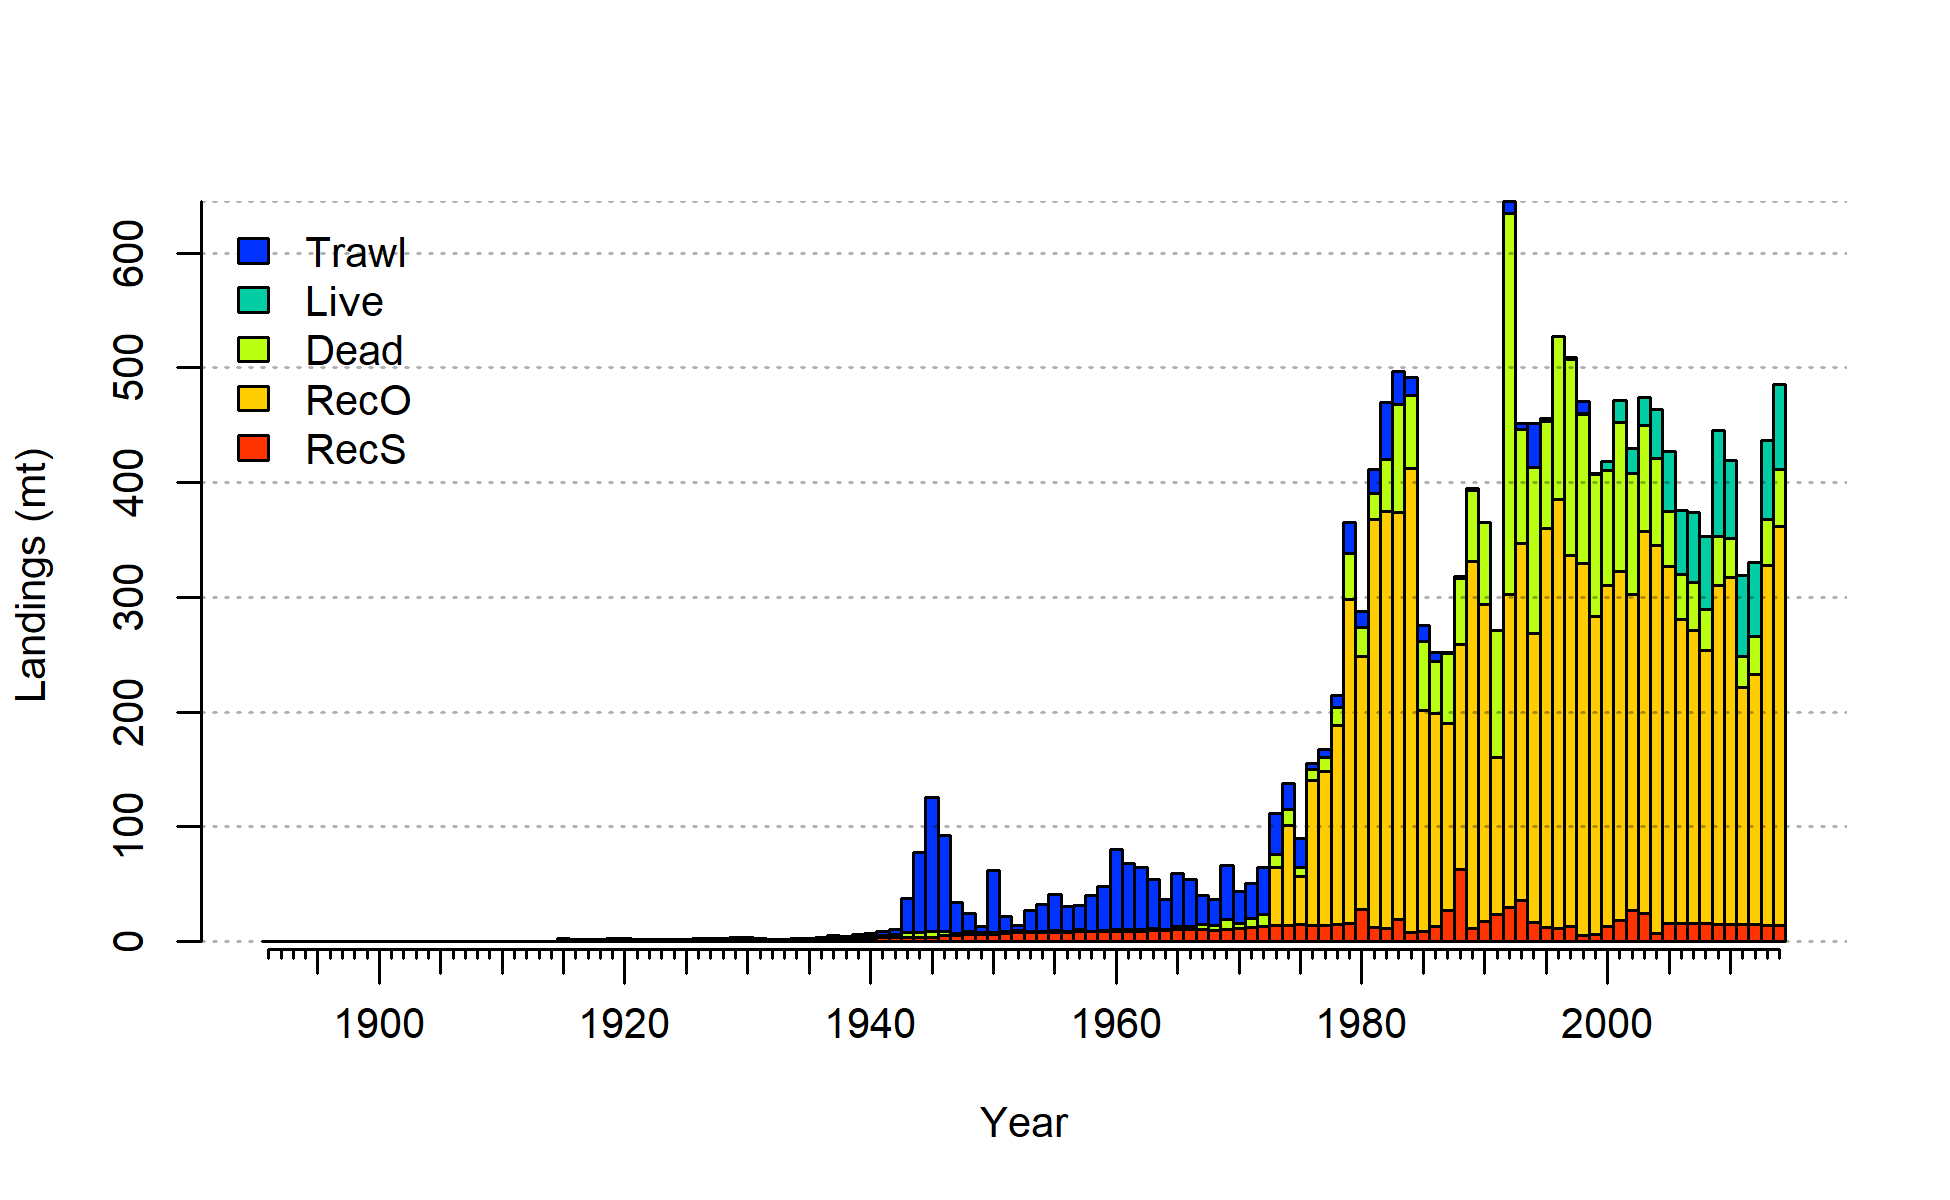
\includegraphics[width=1\textwidth,height=1\textheight]{C:/Users/Jason.Cope/Documents/Github/Sebastes_melanops_WA/Document/models/Reference model/plots/catch2 landings stacked.png}
\caption{Landings by fleet used in the reference model where catches in metric tons by fleet are stacked.\label{fig:es-catch}}
\end{figure}

\clearpage

\hypertarget{data-and-assessment}{%
\subsection*{Data and assessment}\label{data-and-assessment}}
\addcontentsline{toc}{subsection}{Data and assessment}

The first Black Rockfish stock assessment along the West Coast of the U.S. that included the majority of Oregon waters was completed in 1994, covering the area south of Cape Falcon, Oregon to north of Point Piedros Blancos, California (Sampson 2007). The first assessment for waters off Washington was done in 1994, with additional stock assessments in 1999 and 2007. In 2015, a subsequent assessment was completed that included Washington waters only as one of three (also Oregon and California) separate assessment areas delineated by state lines (Cope et al. 2016). Similarly, this assessment treats Washington waters as a single assessment area. The previous two assessments used Stock Synthesis software, as does this one (version 3.30.21.00).

This assessment integrates data and information from multiple sources into one modeling framework. The stock assessment model for Black Rockfish is informed by catch data from two commercial fleets and one recreational fleet, six abundance indices, length composition data from commercial, recreational, and surveys, and conditional age-at-length compositions from the commercial and recreational fisheries. It also uses two ageing error matrices to incorporate ageing imprecision and applies fixed parameterizations of weight-at-length, maturity-at-length, fecundity-at-length, the Beverton-Holt stock-recruitment steepness value, and recruitment variability. Life history parameters were sex-specific (i.e., a two-sex model) with natural mortality fixed at estimates from the previous assessment (but rationalized through life history theory) and most growth and recruitment parameters estimated. Additional parameters that were estimated include initial population scale (\(lnR_0\)), selectivity for each fishery and survey, and added survey variance. The base model was tuned to account for the weighting of the length and age data and index variances (with estimated added variance as needed), as well as the specification of the recruitment bias adjustments. Derived quantities include, among other things, the time series of spawning biomass, age and size structure, and current and projected future stock status. The model covers the years 1940 to 2022, with a 12 year forecast beginning in 2023.

Within model uncertainty is explicitly included in this assessment by parameter estimation uncertainty, while among model uncertainty is explored through sensitivity analyses addressing alternative input assumptions such as data treatment and weighting, and model specification sensitivity to the treatment of life history parameters, selectivity, recruitment, and survey catchability. A reference model was selected that best fit the observed data while concomitantly balancing the desire to capture the central tendency across those sources of uncertainty, ensure model realism and tractability, and promote robustness to potential model misspecification.

\hypertarget{stock-biomass-and-dynamics}{%
\subsection*{Stock biomass and dynamics}\label{stock-biomass-and-dynamics}}
\addcontentsline{toc}{subsection}{Stock biomass and dynamics}

Spawning output (in millions of eggs; meggs) instead of spawning biomass is used to report the functionally mature population scale because fecundity is nonlinearly related to body female weight. The estimated spawning output at the beginning of 2023 was 440 meggs (\textasciitilde95 percent asymptotic intervals: 267 to 613 meggs, Table \ref{tab:ssbES} and Figure \ref{fig:es-ssb}), which when compared to unfished spawning output (950) meggs gives a relative stock status level of 46 percent (\textasciitilde95 percent asymptotic intervals: 31 to 61 percent, Figure \ref{fig:es-depl}). Overall, spawning output declined with the onset of commercial fishing, further decreasing with the increasing recreational removals in the 1980s and continued to decline until the commercial fisheries were shutdown in the late 1990s. Notable recent estimated recruitment pulses occurred in 2000, 2008, and 2011. A decade of positive recruitments of varying strengths support a increase in the time series despite recent lower recruitment deviations. The minimum relative stock size of 17 percent of unfished levels is estimated to have occurred in 1995. The stock may have been below the overfished threshold in the 1980s. Currently, the stock is estimated to be above the management target of \(SO_{40\%}\) in 2023 and is estimated to have surpassed the target only recently (Table \ref{tab:ssbES} and Figure \ref{fig:es-depl}).

\begingroup\fontsize{10}{12}\selectfont
\begingroup\fontsize{10}{12}\selectfont

\begin{longtable}[t]{r>{\centering\arraybackslash}p{1.57cm}>{\centering\arraybackslash}p{1.57cm}>{\centering\arraybackslash}p{1.57cm}>{\centering\arraybackslash}p{1.57cm}>{\centering\arraybackslash}p{1.57cm}>{\centering\arraybackslash}p{1.57cm}}
\caption{\label{tab:ssbES}Estimated recent trend in spawning output and the fraction unfished and the 95 percent intervals.}\\
\toprule
Year & Spawning Output & Lower Interval & Upper Interval & Fraction Unfished & Lower Interval & Upper Interval\\
\midrule
\endfirsthead
\caption[]{Estimated recent trend in spawning output and the fraction unfished and the 95 percent intervals. \textit{(continued)}}\\
\toprule
Year & Spawning Output & Lower Interval & Upper Interval & Fraction Unfished & Lower Interval & Upper Interval\\
\midrule
\endhead

\endfoot
\bottomrule
\endlastfoot
2013 & 239.61 & 189.29 & 289.93 & 0.25 & 0.21 & 0.29\\
2014 & 249.53 & 192.38 & 306.68 & 0.26 & 0.22 & 0.31\\
2015 & 261.05 & 195.22 & 326.88 & 0.27 & 0.22 & 0.33\\
2016 & 274.76 & 198.39 & 351.13 & 0.29 & 0.23 & 0.35\\
2017 & 289.73 & 200.98 & 378.47 & 0.31 & 0.23 & 0.38\\
2018 & 319.12 & 216.03 & 422.21 & 0.34 & 0.25 & 0.42\\
2019 & 346.49 & 227.88 & 465.10 & 0.36 & 0.27 & 0.46\\
2020 & 372.63 & 238.20 & 507.06 & 0.39 & 0.28 & 0.51\\
2021 & 406.97 & 257.39 & 556.55 & 0.43 & 0.30 & 0.56\\
2022 & 425.64 & 263.13 & 588.16 & 0.45 & 0.31 & 0.59\\
2023 & 439.55 & 266.93 & 612.16 & 0.46 & 0.31 & 0.61\\*
\end{longtable}
\endgroup{}
\endgroup{}


\begin{figure}
\centering
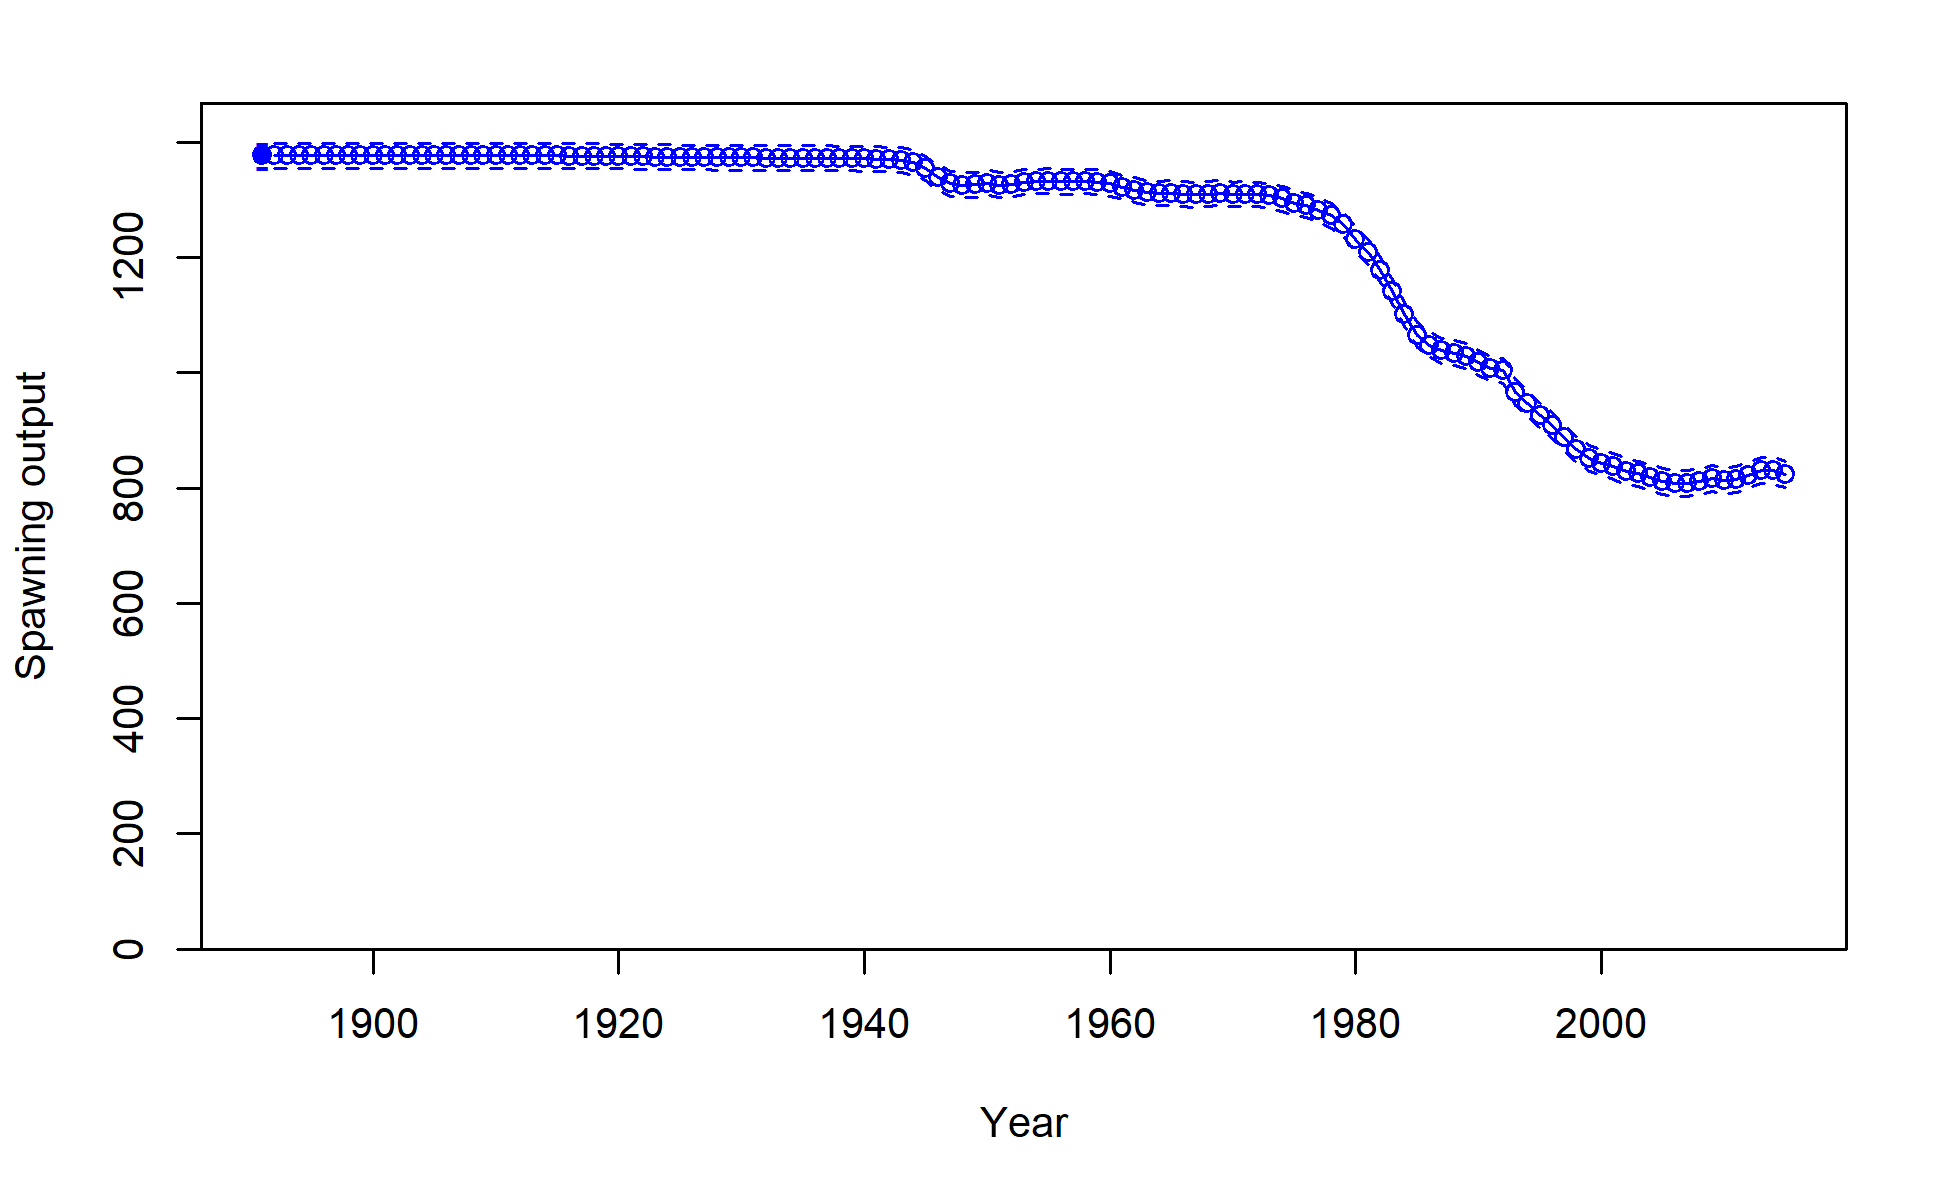
\includegraphics[width=1\textwidth,height=1\textheight]{C:/Users/Jason.Cope/Documents/Github/Sebastes_melanops_WA/Document/models/Reference model/plots/ts7_Spawning_output_with_95_asymptotic_intervals_intervals.png}
\caption{Estimated time series of spawning output (circles and line: median; light broken lines: 95 percent intervals) for the base model.\label{fig:es-ssb}}
\end{figure}

\begin{figure}
\centering
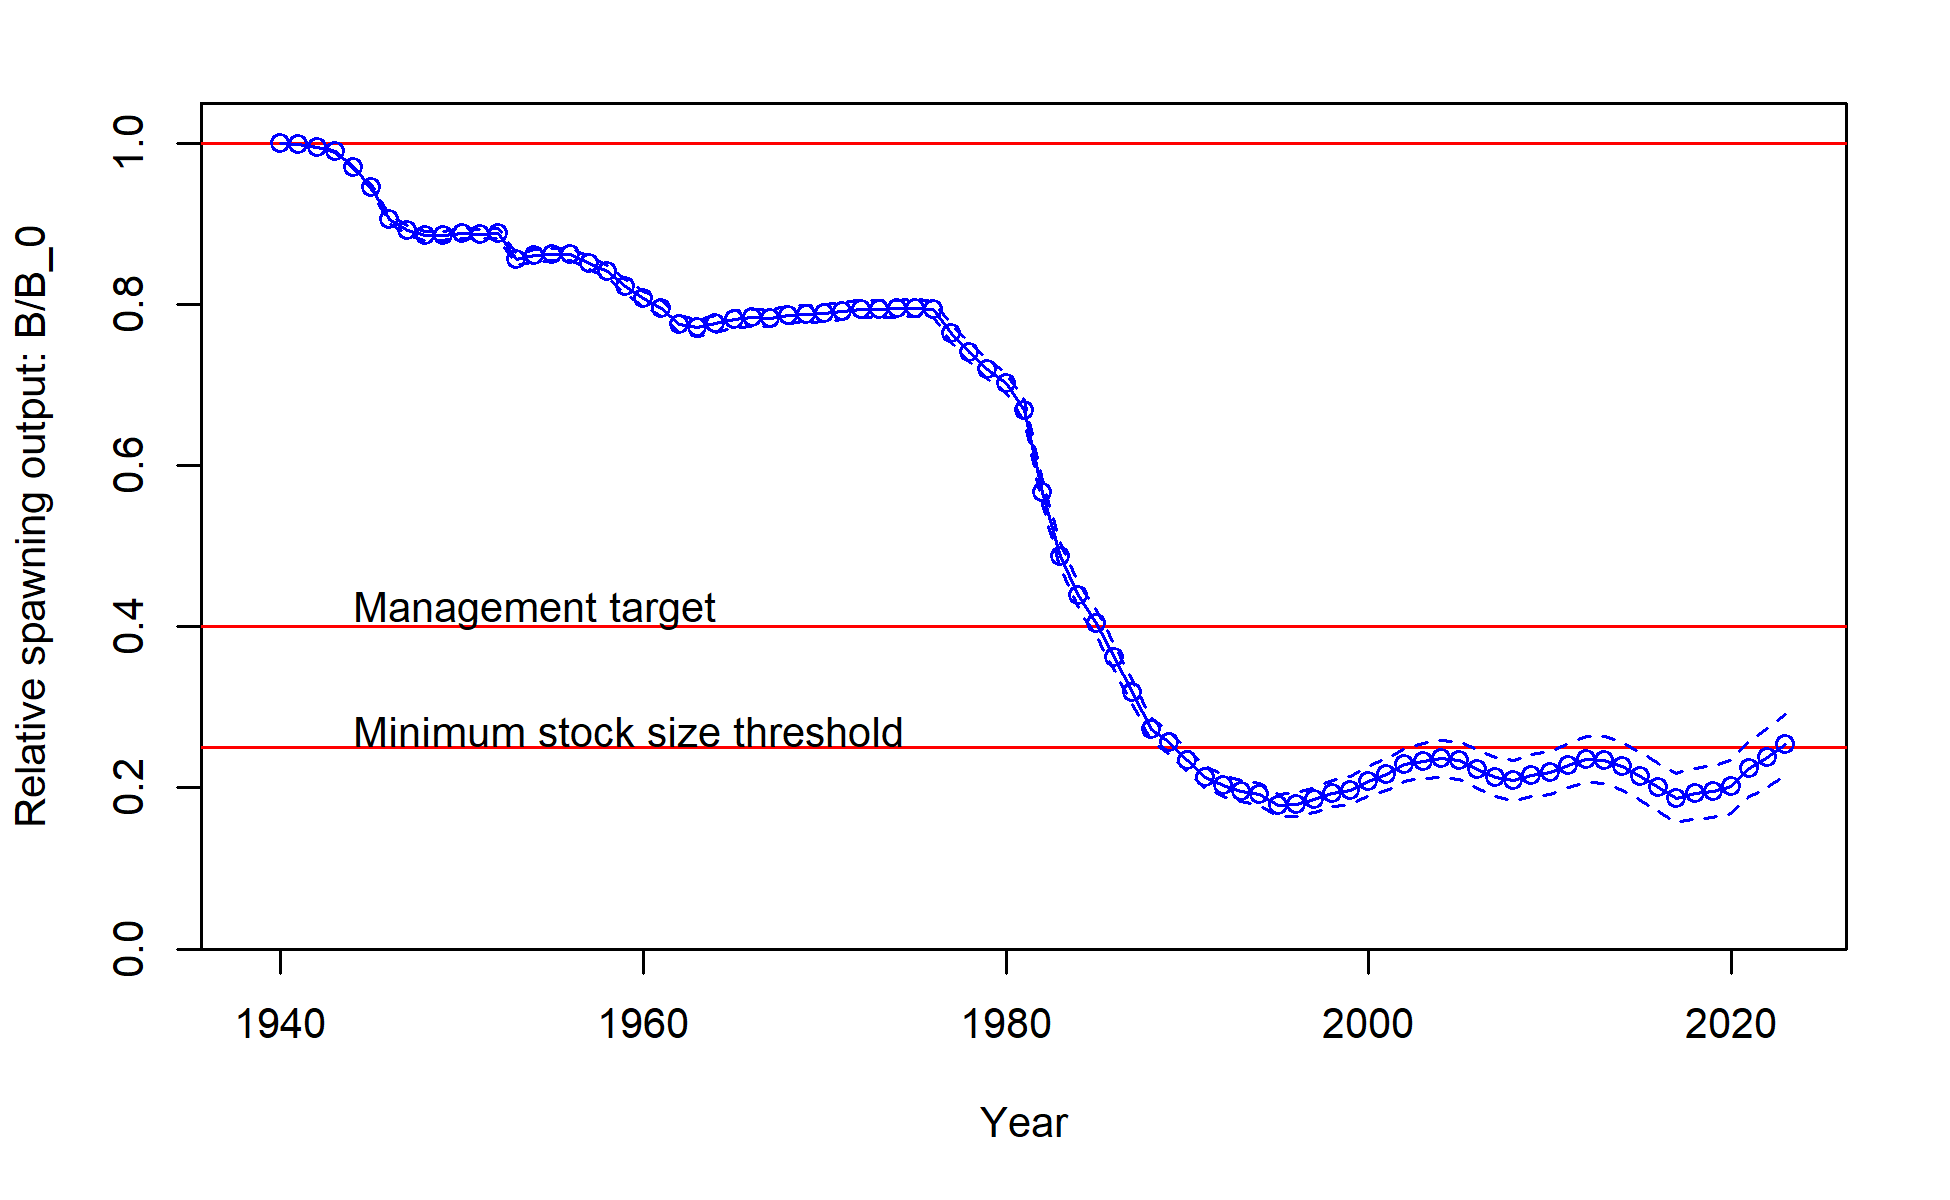
\includegraphics[width=1\textwidth,height=1\textheight]{C:/Users/Jason.Cope/Documents/Github/Sebastes_melanops_WA/Document/models/Reference model/plots/ts9_Relative_spawning_output_intervals.png}
\caption{Estimated time series of fraction of unfished spawning output (circles and line: median; light broken lines: 95 percent intervals) for the base model.\label{fig:es-depl}}
\end{figure}

\clearpage

\hypertarget{recruitment}{%
\subsection*{Recruitment}\label{recruitment}}
\addcontentsline{toc}{subsection}{Recruitment}

Recruitment is informed by the data and estimated from 1970s to 2017, before and after which it is assumed taken from the stock-recruit relationship (Table \ref{tab:recrES} and Figure \ref{fig:es-recruits}). The highest recruitment years occurred in 2000, 2008, and 2011. The large 2008 and 2011 year classes, as well as several above average year classes in the mid 2000s to early 2010s, contributed to the recent increase in Black Rockfish biomass. Recruitment is informed mostly by the composition data. While the Black Rockfish stock has been reduced to levels that theoretically would provide some information on how recruitment compensation changes across spawning biomass levels (i.e., inform the steepness parameter), the assessment model could not adequately estimate a reasonable steepness parameter given that most of the data was collected after the major decline in the spawning output and/or did not show much contrast. Thus, recruitment is based on a fixed assumption about steepness (\(h\) = 0.72) and recruitment variability (\(\sigma_R\) = 0.6).

\begingroup\fontsize{10}{12}\selectfont
\begingroup\fontsize{10}{12}\selectfont

\begin{longtable}[t]{r>{\centering\arraybackslash}p{1.57cm}>{\centering\arraybackslash}p{1.57cm}>{\centering\arraybackslash}p{1.57cm}>{\centering\arraybackslash}p{1.57cm}>{\centering\arraybackslash}p{1.57cm}>{\centering\arraybackslash}p{1.57cm}}
\caption{\label{tab:recrES}Estimated recent trend in recruitment and recruitment deviations and the 95 percent intervals.}\\
\toprule
Year & Recruitment & Lower Interval & Upper Interval & Recruitment Deviations & Lower Interval & Upper Interval\\
\midrule
\endfirsthead
\caption[]{Estimated recent trend in recruitment and recruitment deviations and the 95 percent intervals. \textit{(continued)}}\\
\toprule
Year & Recruitment & Lower Interval & Upper Interval & Recruitment Deviations & Lower Interval & Upper Interval\\
\midrule
\endhead

\endfoot
\bottomrule
\endlastfoot
2013 & 1972.96 & 1304.38 & 2984.22 & 0.42 & 0.08 & 0.77\\
2014 & 1524.90 & 970.90 & 2395.02 & 0.15 & -0.23 & 0.54\\
2015 & 1117.78 & 678.00 & 1842.81 & -0.17 & -0.61 & 0.27\\
2016 & 1222.12 & 732.14 & 2040.03 & -0.12 & -0.57 & 0.34\\
2017 & 745.60 & 383.36 & 1450.13 & -0.65 & -1.28 & -0.02\\
2018 & 1640.14 & 1429.19 & 1882.23 & 0.00 & 0.00 & 0.00\\
2019 & 1671.35 & 1454.43 & 1920.62 & 0.00 & 0.00 & 0.00\\
2020 & 1697.60 & 1475.50 & 1953.13 & 0.00 & 0.00 & 0.00\\
2021 & 1728.44 & 1505.90 & 1983.87 & 0.00 & 0.00 & 0.00\\
2022 & 1742.76 & 1516.49 & 2002.79 & 0.00 & 0.00 & 0.00\\
2023 & 1752.52 & 1523.38 & 2016.13 & 0.00 & 0.00 & 0.00\\*
\end{longtable}
\endgroup{}
\endgroup{}


\begin{figure}
\centering
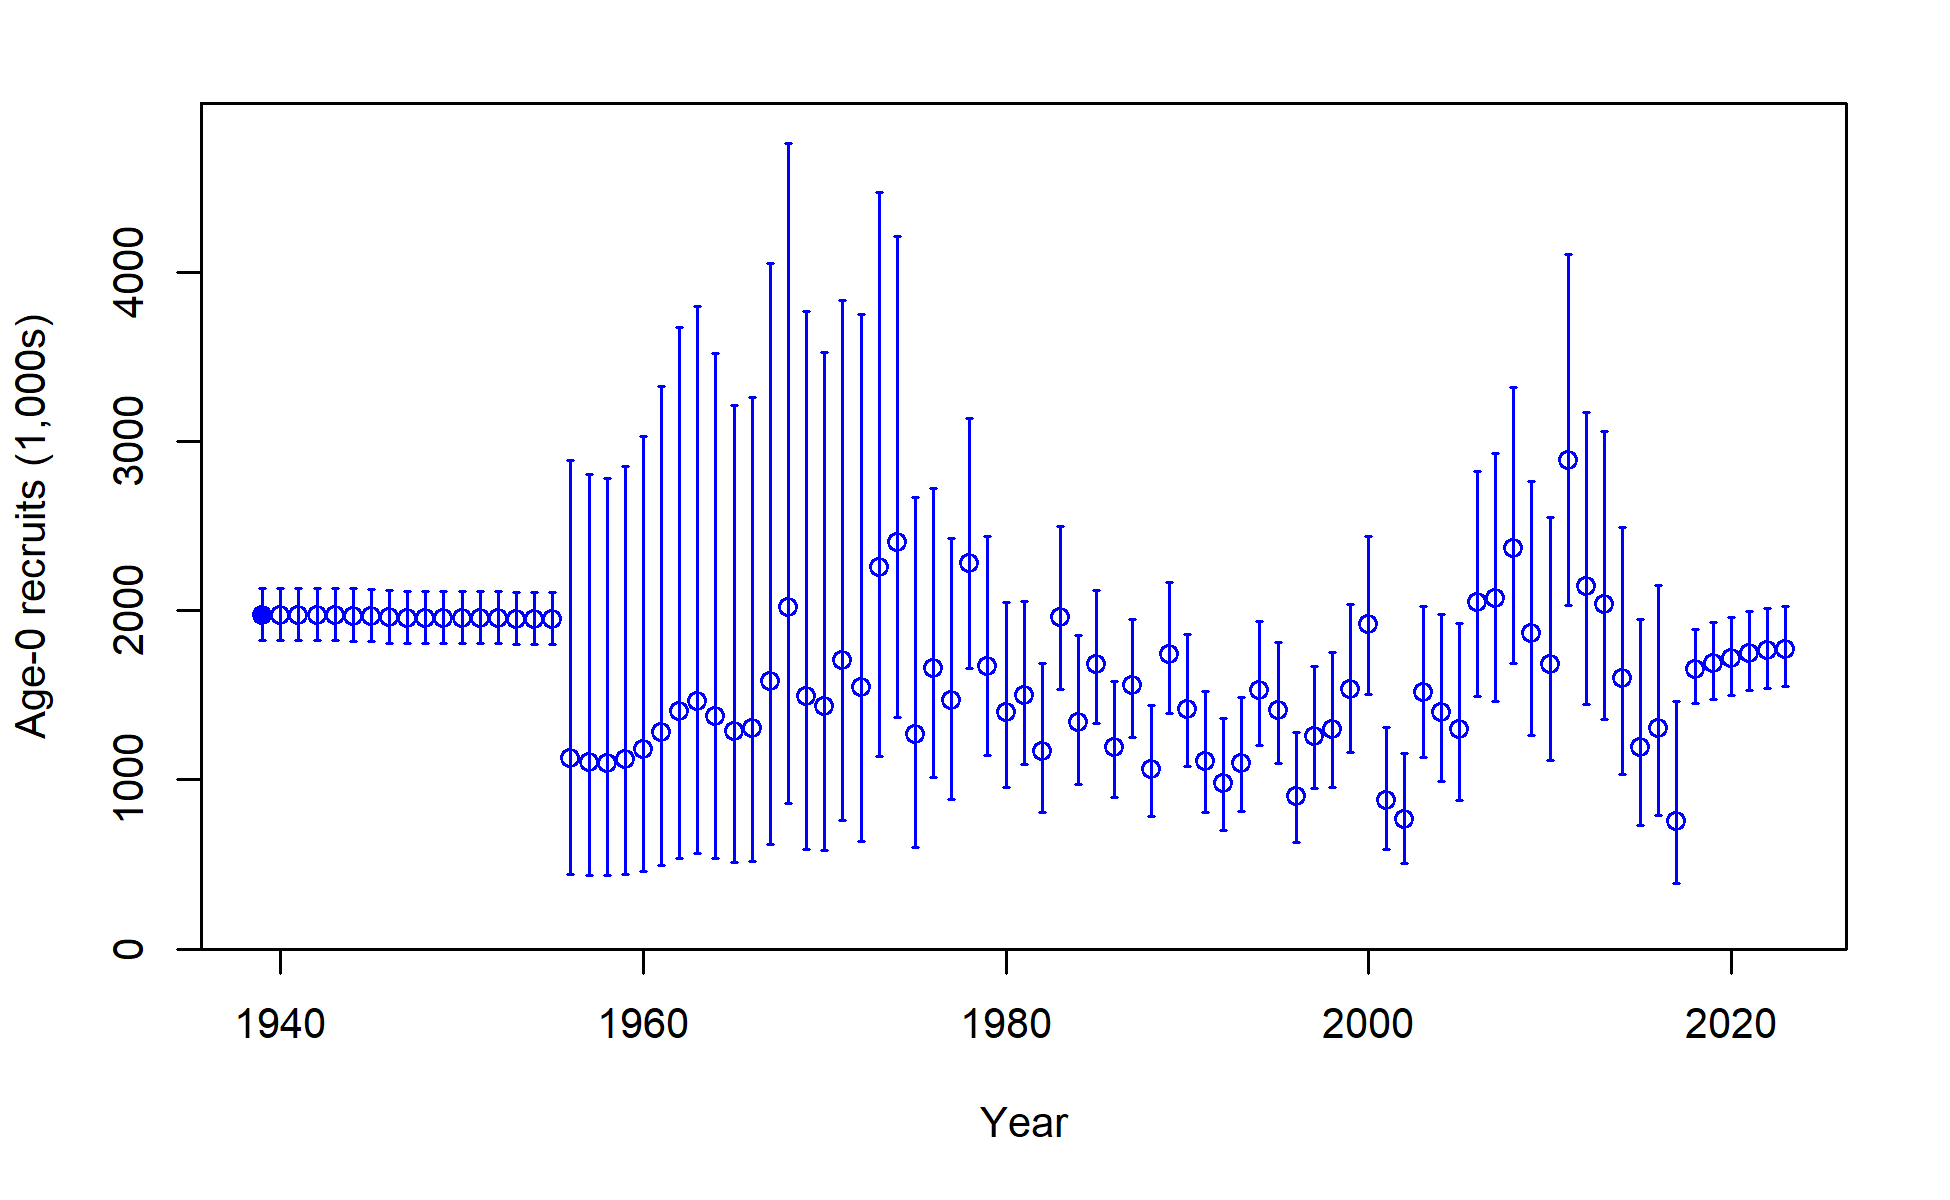
\includegraphics[width=1\textwidth,height=1\textheight]{C:/Users/Jason.Cope/Documents/Github/Sebastes_melanops_WA/Document/models/Reference model/plots/ts11_Age-0_recruits_(1000s)_with_95_asymptotic_intervals.png}
\caption{Estimated time series of age-0 recruits (1000s) for the base model with 95 percent intervals.\label{fig:es-recruits}}
\end{figure}

\begin{figure}
\centering
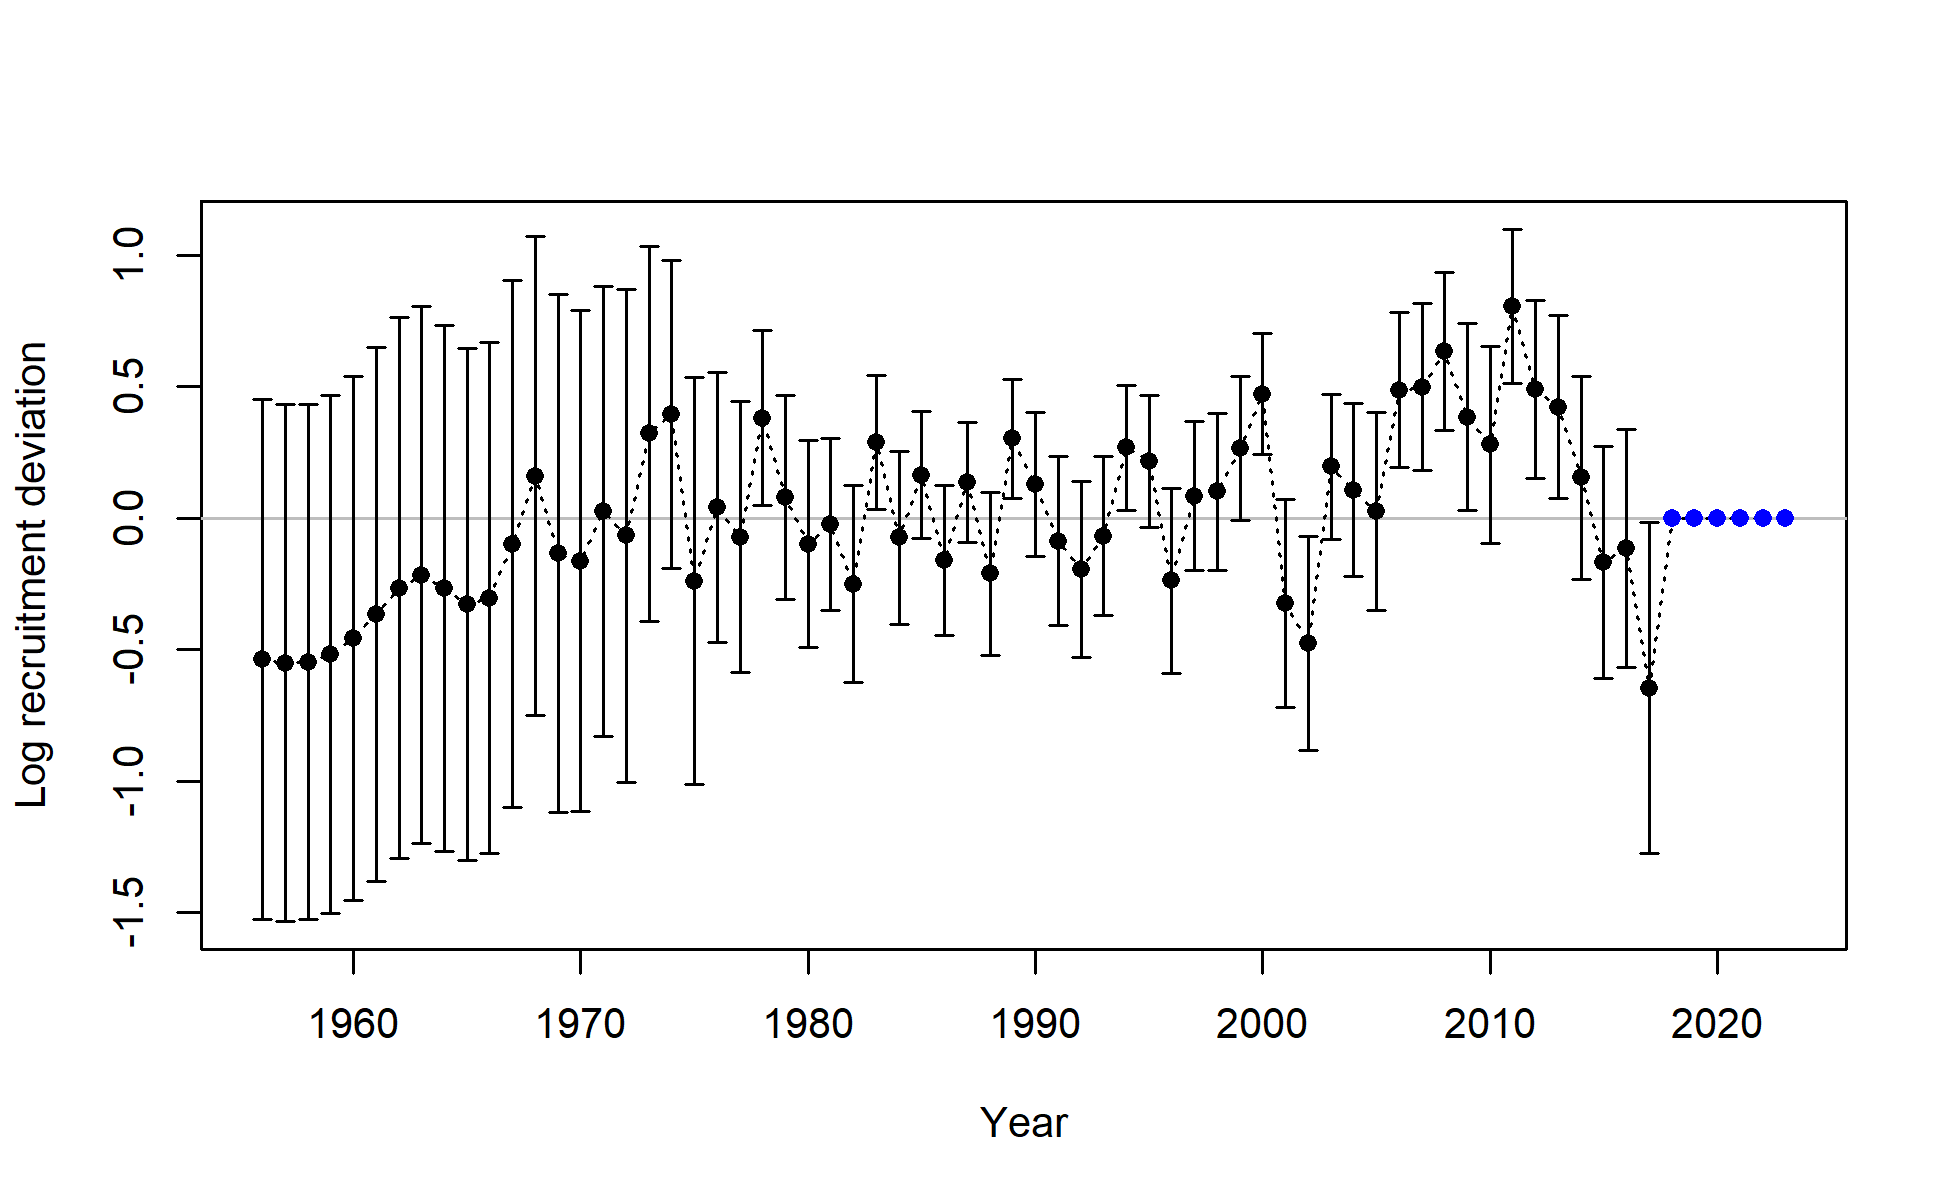
\includegraphics[width=1\textwidth,height=1\textheight]{C:/Users/Jason.Cope/Documents/Github/Sebastes_melanops_WA/Document/models/Reference model/plots/recdevs2_withbars.png}
\caption{Estimated time series of recruitment deviations.\label{fig:es-recdev}}
\end{figure}

\hypertarget{exploitation-status}{%
\subsection*{Exploitation status}\label{exploitation-status}}
\addcontentsline{toc}{subsection}{Exploitation status}

Fishing intensity, as measured by the SPR rate (1 - SPR), has remained high and above the target of 50\% since the 1980s and only recently dropped below the target (1 - \(\text{SPR}_{50\%}\)). Highest fishing rates were in the 1980s to mid 1990s after which is started to drop (Table \ref{tab:exploitES} and Figures \ref{fig:es-1-spr} and \ref{fig:es-phase}). The steepness value of 0.72 indicates that a lower value of SPR (or equivalently a higher fishing intensity than \(\text{SPR}_{50\%}\)) would be consistent with the biomass-based target of (\(\text{SO}_{40\%}\)) for sustainable removals. Trends in fishing intensity largely mirrored that of landings until the 1990s, after which recruitment pulses countered the catches somewhat to lower overall fishing intensity (Figure \ref{fig:es-1-spr}). The maximum fishing intensity was 0.8 in 1994, which is well above the target SPR-based harvest rate of 0.50. The current level of 0.41 for 2022 is below that target. Fishing intensity over the past decade has ranged between 0.31 and 0.66 and the exploitation rate (range of 0.02 - 0.07, Table \ref{tab:exploitES}) has come down since the mid-1990s. Current estimates indicate that Black Rockfish spawning output is greater than the target biomass level (\(\text{SO}_{40\%}\)), though fishing intensity remains near the target \(F_{MSY}\) proxy harvest rate of 1 - \(\text{SPR}_{50\%}\) (Figure \ref{fig:es-phase}).

\begingroup\fontsize{10}{12}\selectfont
\begingroup\fontsize{10}{12}\selectfont

\begin{longtable}[t]{r>{\centering\arraybackslash}p{1.57cm}>{\centering\arraybackslash}p{1.57cm}>{\centering\arraybackslash}p{1.57cm}>{\centering\arraybackslash}p{1.57cm}>{\centering\arraybackslash}p{1.57cm}>{\centering\arraybackslash}p{1.57cm}}
\caption{\label{tab:exploitES}Estimated recent trend in the 1-SPR where SPR is the spawning potential ratio the exploitation rate, and the  95 percent intervals.}\\
\toprule
Year & 1-SPR & Lower Interval & Upper Interval & Exploitation Rate & Lower Interval & Upper Interval\\
\midrule
\endfirsthead
\caption[]{Estimated recent trend in the 1-SPR where SPR is the spawning potential ratio the exploitation rate, and the  95 percent intervals. \textit{(continued)}}\\
\toprule
Year & 1-SPR & Lower Interval & Upper Interval & Exploitation Rate & Lower Interval & Upper Interval\\
\midrule
\endhead

\endfoot
\bottomrule
\endlastfoot
2013 & 0.65 & 0.60 & 0.71 & 0.06 & 0.05 & 0.08\\
2014 & 0.67 & 0.60 & 0.73 & 0.07 & 0.05 & 0.08\\
2015 & 0.66 & 0.59 & 0.73 & 0.07 & 0.05 & 0.09\\
2016 & 0.65 & 0.57 & 0.73 & 0.07 & 0.05 & 0.09\\
2017 & 0.52 & 0.43 & 0.61 & 0.05 & 0.03 & 0.06\\
2018 & 0.53 & 0.43 & 0.62 & 0.05 & 0.03 & 0.07\\
2019 & 0.50 & 0.40 & 0.59 & 0.05 & 0.03 & 0.07\\
2020 & 0.32 & 0.23 & 0.40 & 0.03 & 0.02 & 0.03\\
2021 & 0.41 & 0.31 & 0.51 & 0.04 & 0.03 & 0.05\\
2022 & 0.37 & 0.27 & 0.46 & 0.03 & 0.02 & 0.04\\*
\end{longtable}
\endgroup{}
\endgroup{}


\begin{figure}
\centering
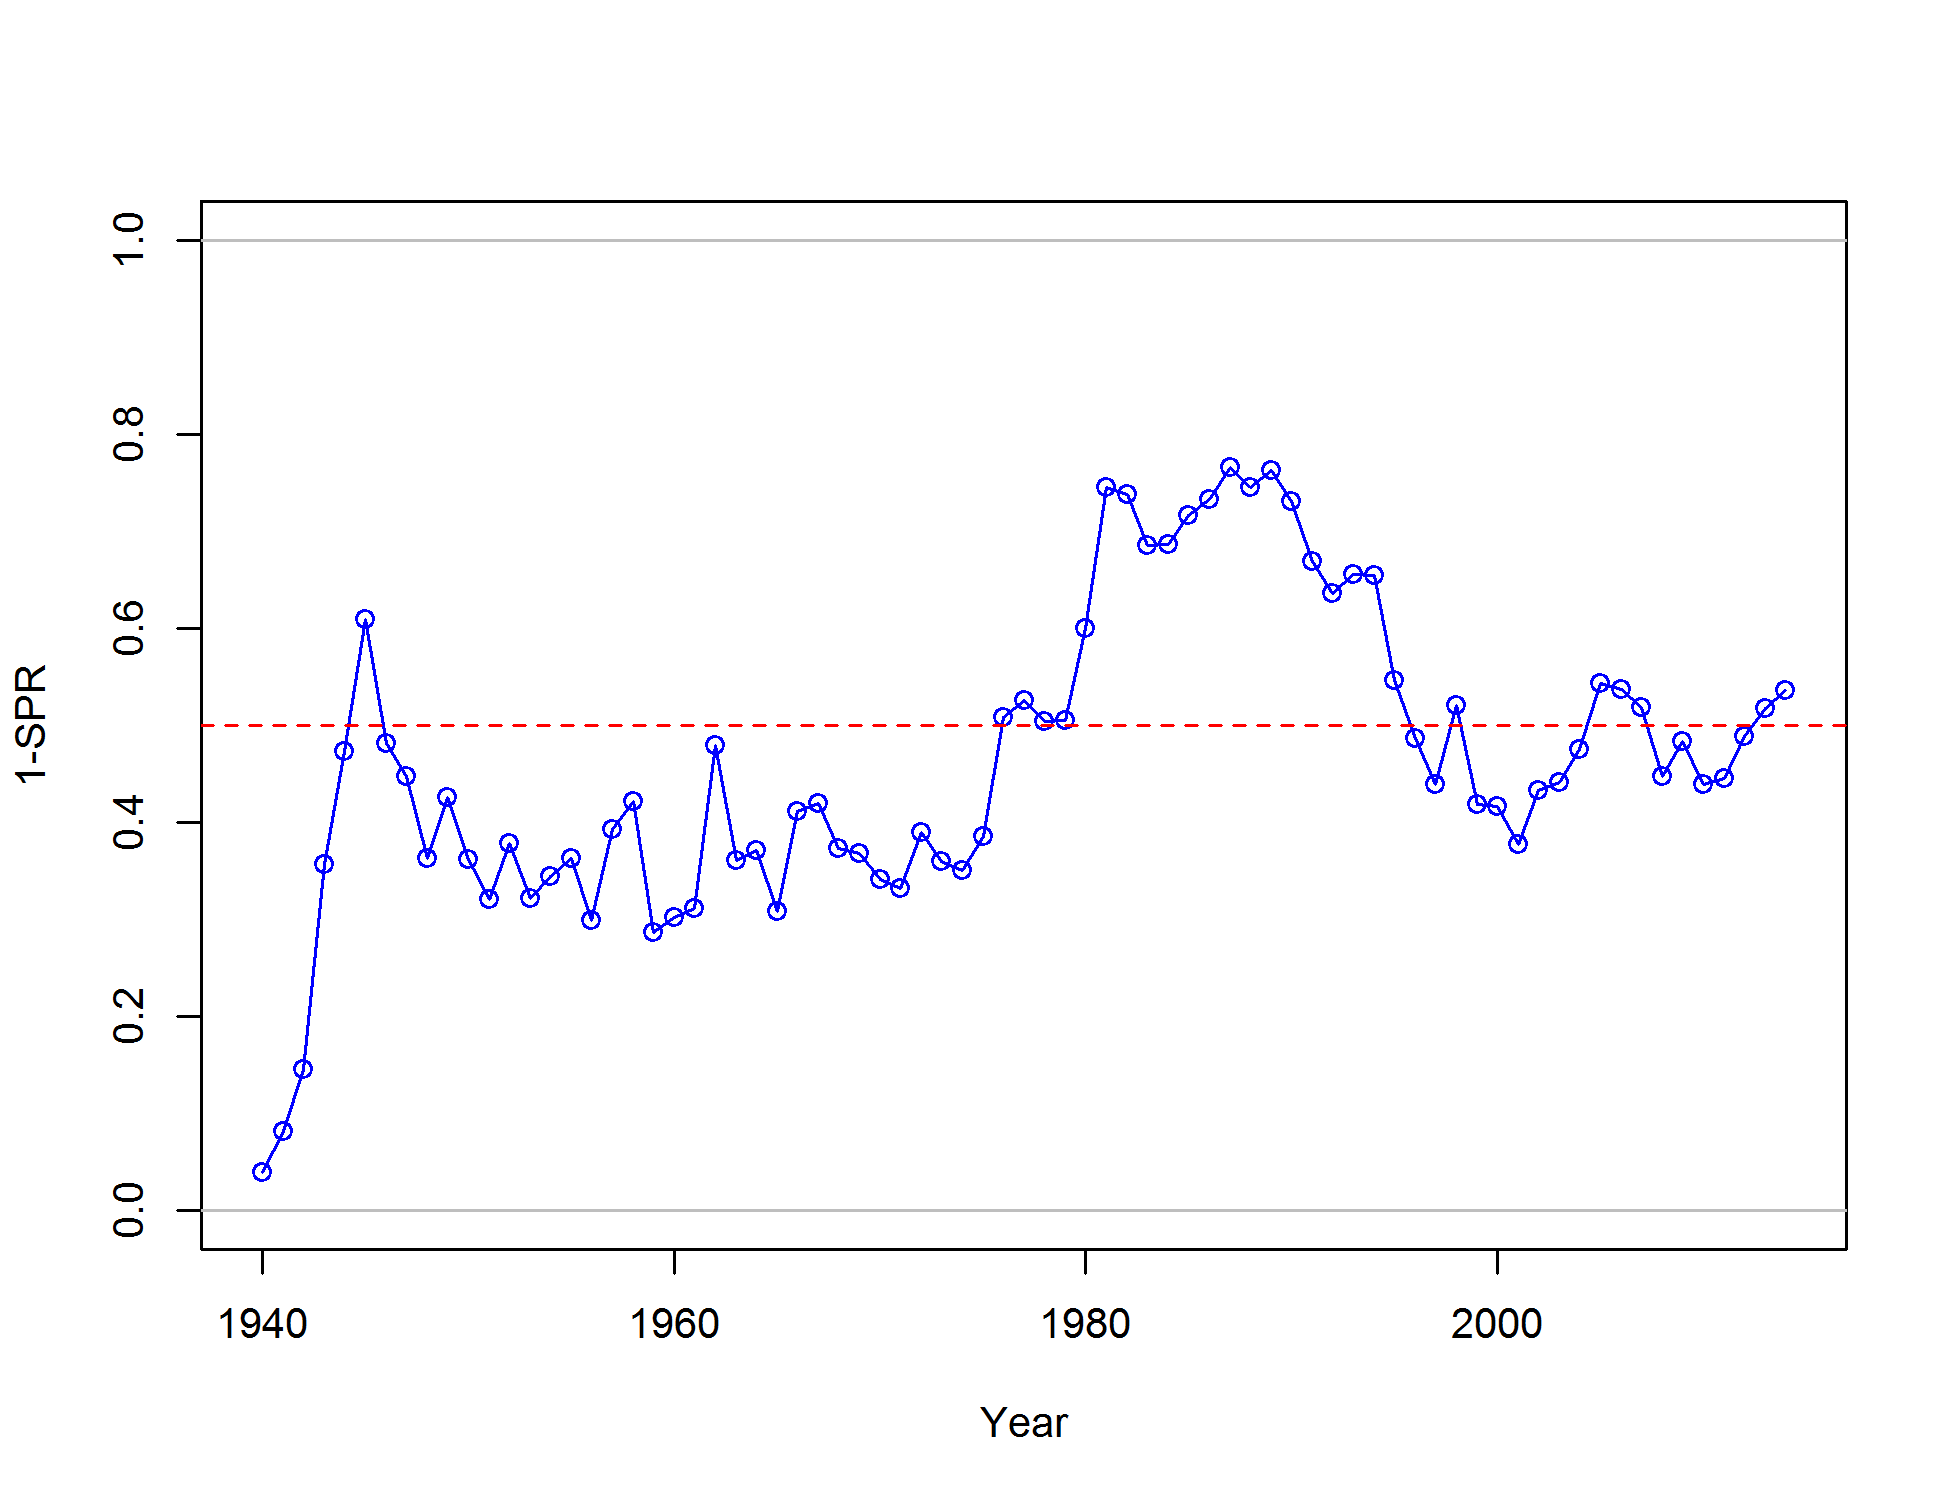
\includegraphics[width=1\textwidth,height=1\textheight]{C:/Users/Jason.Cope/Documents/Github/Sebastes_melanops_WA/Document/models/Reference model/plots/SPR2_minusSPRseries.png}
\caption{Estimated 1 - relative spawning ratio (SPR) by year for the base model. The management target is plotted as a red horizontal line and values above this reflect harvest in excess of the proxy harvest rate.\label{fig:es-1-spr}}
\end{figure}

\clearpage

\hypertarget{ecosystem-considerations}{%
\subsection*{Ecosystem considerations}\label{ecosystem-considerations}}
\addcontentsline{toc}{subsection}{Ecosystem considerations}

This stock assessment does not explicitly incorporate trophic interactions, habitat factors, or environmental factors into the assessment model. More predation, diet and habitat work, and mechanistic linkages to environmental conditions would be needed to incorporate these elements into the stock assessment and should remain a priority. McClure et al. (2023) report the climate vulnerability for several west coast groundfishes, including Black Rockfish. Black Rockfish demonstrated both high biological sensitivity and high climate exposure risk, to give it an overall high vulnerability score to climate change. This result should also be considered with the fact that, like many rockfishes, periods of low productivity is not unusual to Black Rockfish and their extended longevity (though admittedly this seems shorter than previously believed and should be reconsidered) has historically allowed them to wait for advantageous productivity periods. Additional stressors such as fishing and climate change that possibly truncate longevity could bring significant challenges to population sustainability.

\hypertarget{reference-points}\)), target relative biomass (40\%), and estimated selectivity and catch for each fleet (Table \ref{tab:referenceES}). The Black Rockfish population in Washington at the start of 2023 is estimated to be just above the target biomass, and fishing intensity during 2022 is estimated to be just below the fishing intensity target (Figure \ref{fig:es-phase}). The yield values are lower than the previous assessment for similar reference points due to updated life history estimates and estimates of the total scale of the population, despite the overall stock status being a bit higher. The proxy MSY values of management quantities are by definition more conservative compared to the estimated MSY and MSY relative to 40\% of unfished spawning output because of the assumed steepness value. Sustainable total yield, removals, using the proxy \(\text{SPR}_{50\%}\) is 278 mt. The spawning output equivalent to 40\% of the unfished spawning output (\(\text{SO}_{40\%}\)) calculated using the SPR target (\(\text{SPR}_{50\%}\)) was 423.7 millions of eggs.

Recent removals since 2017 have been at or below the point estimate of potential long-term yields calculated using an \(\text{SPR}_{50\%}\) reference point, leading to a population that has continued to increase over recent years with the assistance of above average recruitment between 2003-2014, despite below average recruitment starting in 2015. The equilibrium estimates of yield relative to biomass based on a steepness value fixed at 0.72 are provided in Figure \ref{fig:es-yield}, where vertical dashed lines indicate the estimate of fraction unfished at the start of 2023 (current) and the estimated management targets calculated based on the relative target biomass (B target), the SPR target, and the maximum sustainable yield (MSY).

The 2023 spawning biomass relative to unfished equilibrium spawning biomass, based on the 2022 fishing year, is 46\%, above the management target of 40\% of unfished spawning output. The relative biomass and the ratio of the estimated SPR to the management target (\(\text{SPR}_{50\%}\)) across all model years are shown in Figure \ref{fig:es-phase} where warmer colors (red) represent early years and colder colors (blue) represent recent years. There have been periods where the stock status has decreased below the target and limit relative biomass, and fishing intensity has been higher than the target fishing intensity based on \(\text{SPR}_{50\%}\).

\begingroup\fontsize{10}{12}\selectfont
\begingroup\fontsize{10}{12}\selectfont

\begin{longtable}[t]{r>{\centering\arraybackslash}p{2cm}>{\centering\arraybackslash}p{2cm}}
\caption{\label{tab:referenceES}Summary of reference points and management quantities, including estimates of the  95 percent intervals.}\\
\toprule
 & Estimate & Interval\\
\midrule
\endfirsthead
\caption[]{Summary of reference points and management quantities, including estimates of the  95 percent intervals. \textit{(continued)}}\\
\toprule
 & Estimate & Interval\\
\midrule
\endhead

\endfoot
\bottomrule
\endlastfoot
Unfished Spawning Output & 943.88 & 867.65-1020.10\\
Unfished Age 0+ Biomass (mt) & 8704.38 & 7999.16-9409.60\\
Unfished Recruitment (R0) & 1959.43 & 1801.19-2117.67\\
Spawning Output (2023) & 426.15 & 251.53-600.77\\
Fraction Unfished (2023) & 0.45 & 0.30-0.60\\
\underline{Reference Points Based on SB40\%} & \\
Proxy Spawning Output SB40\% & 377.55 & 347.06-408.04\\
SPR Resulting in SB40\% & 0.46 & 0.46-0.46\\
Exploitation Rate Resulting in SB40\% & 0.05 & 0.05-0.05\\
Yield with SPR Based On SB40\% (mt) & 293.52 & 269.82-317.22\\
\underline{Reference Points Based on SPR Proxy for MSY} &  & \\
Proxy Spawning Output (SPR50) & 421.11 & 387.11-455.12\\
SPR50 & 0.50 & -\\
Exploitation Rate Corresponding to SPR50 & 0.05 & 0.05-0.05\\
Yield with SPR50 at SB SPR (mt) & 275.88 & 253.60-298.17\\
\underline{Reference Points Based on Estimated MSY Values} &  & \\
Spawning Output at MSY (SB MSY) & 212.51 & 195.32-229.69\\
SPR MSY & 0.30 & 0.30-0.30\\
Exploitation Rate Corresponding to SPR MSY & 0.08 & 0.08-0.08\\
MSY (mt) & 332.18 & 305.38-358.98\\*
\end{longtable}
\endgroup{}
\endgroup{}


\begin{figure}
\centering
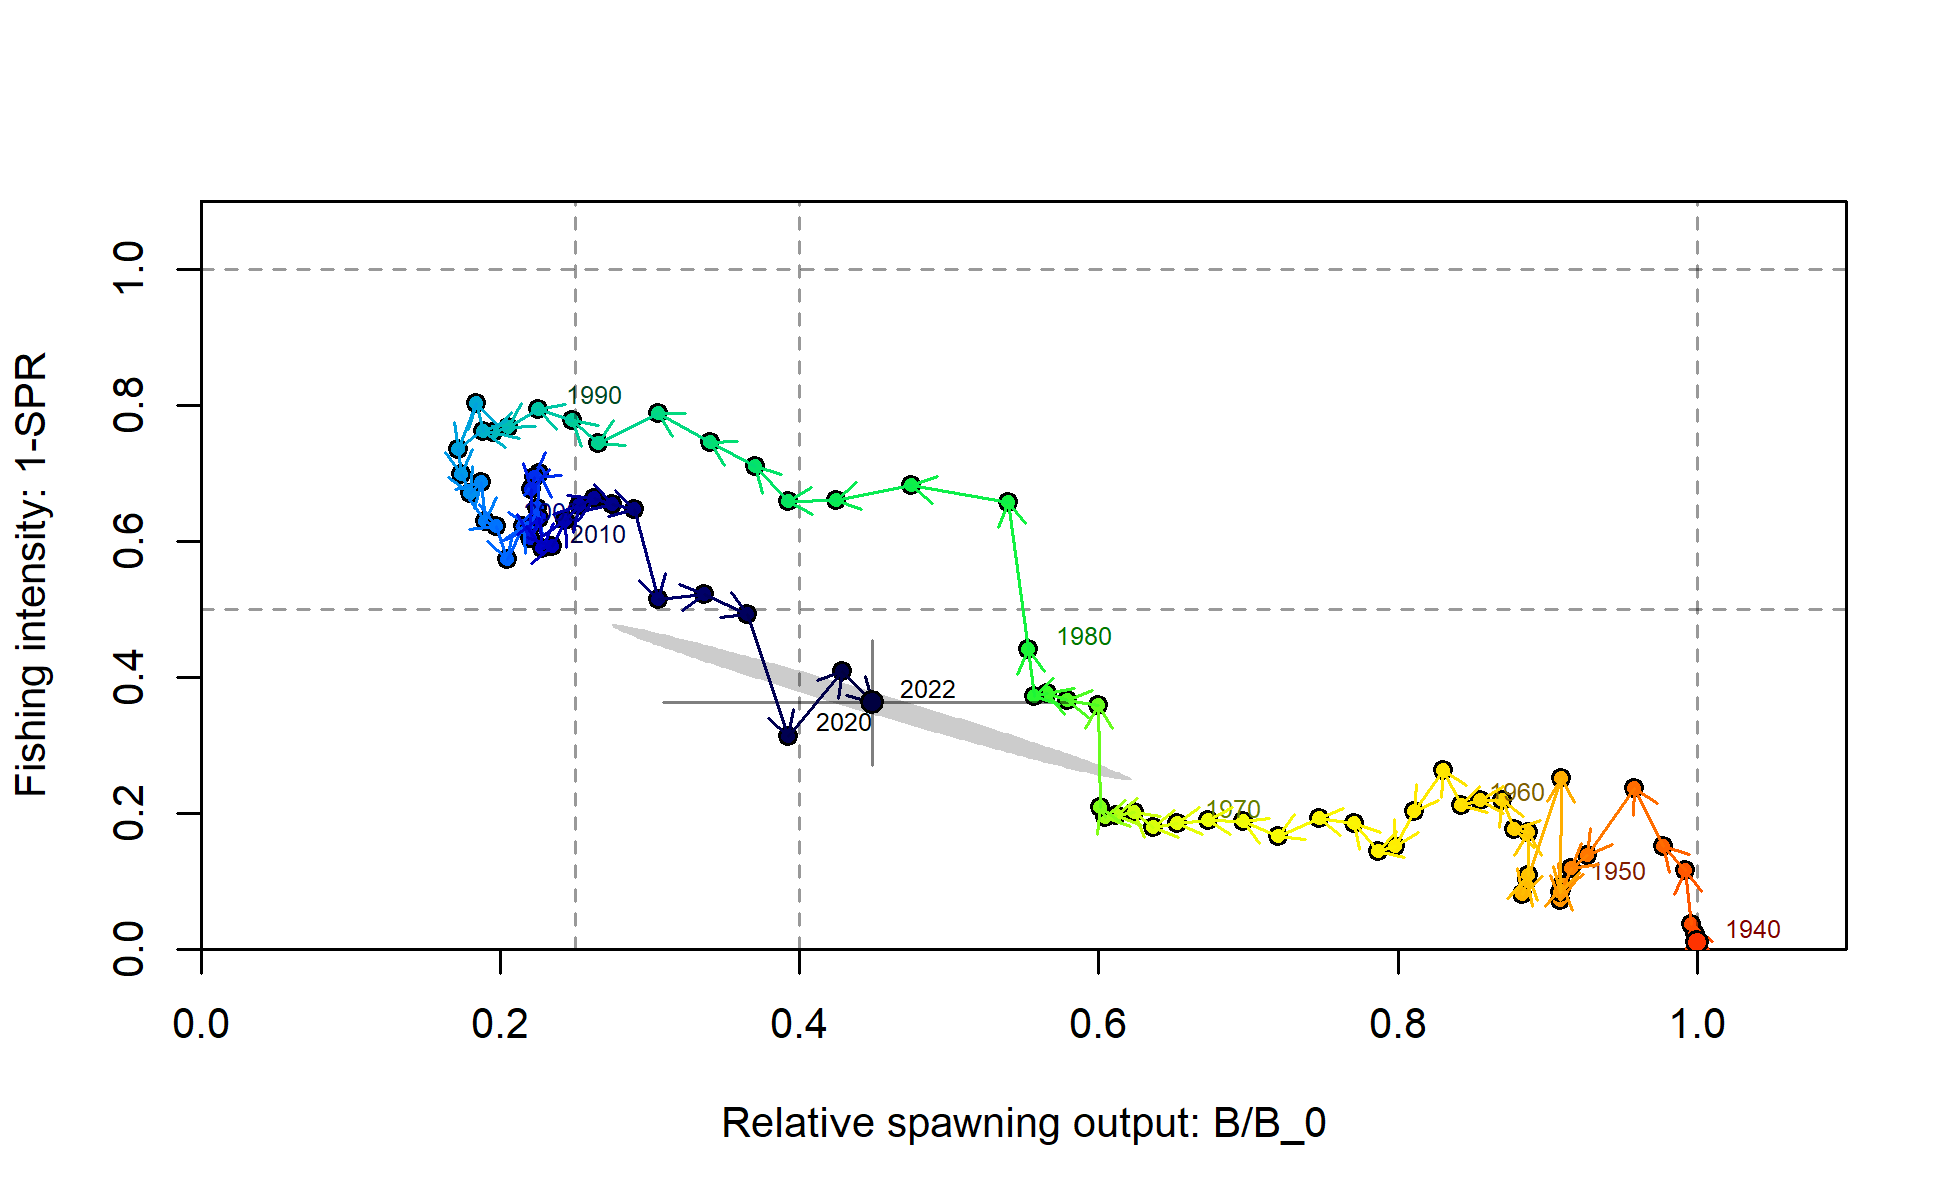
\includegraphics[width=1\textwidth,height=1\textheight]{C:/Users/Jason.Cope/Documents/Github/Sebastes_melanops_WA/Document/models/Reference model/plots/SPR4_phase.png}
\caption{Phase plot of estimated 1-SPR versus fraction unfished for the base model.\label{fig:es-phase}}
\end{figure}

\begin{figure}
\centering
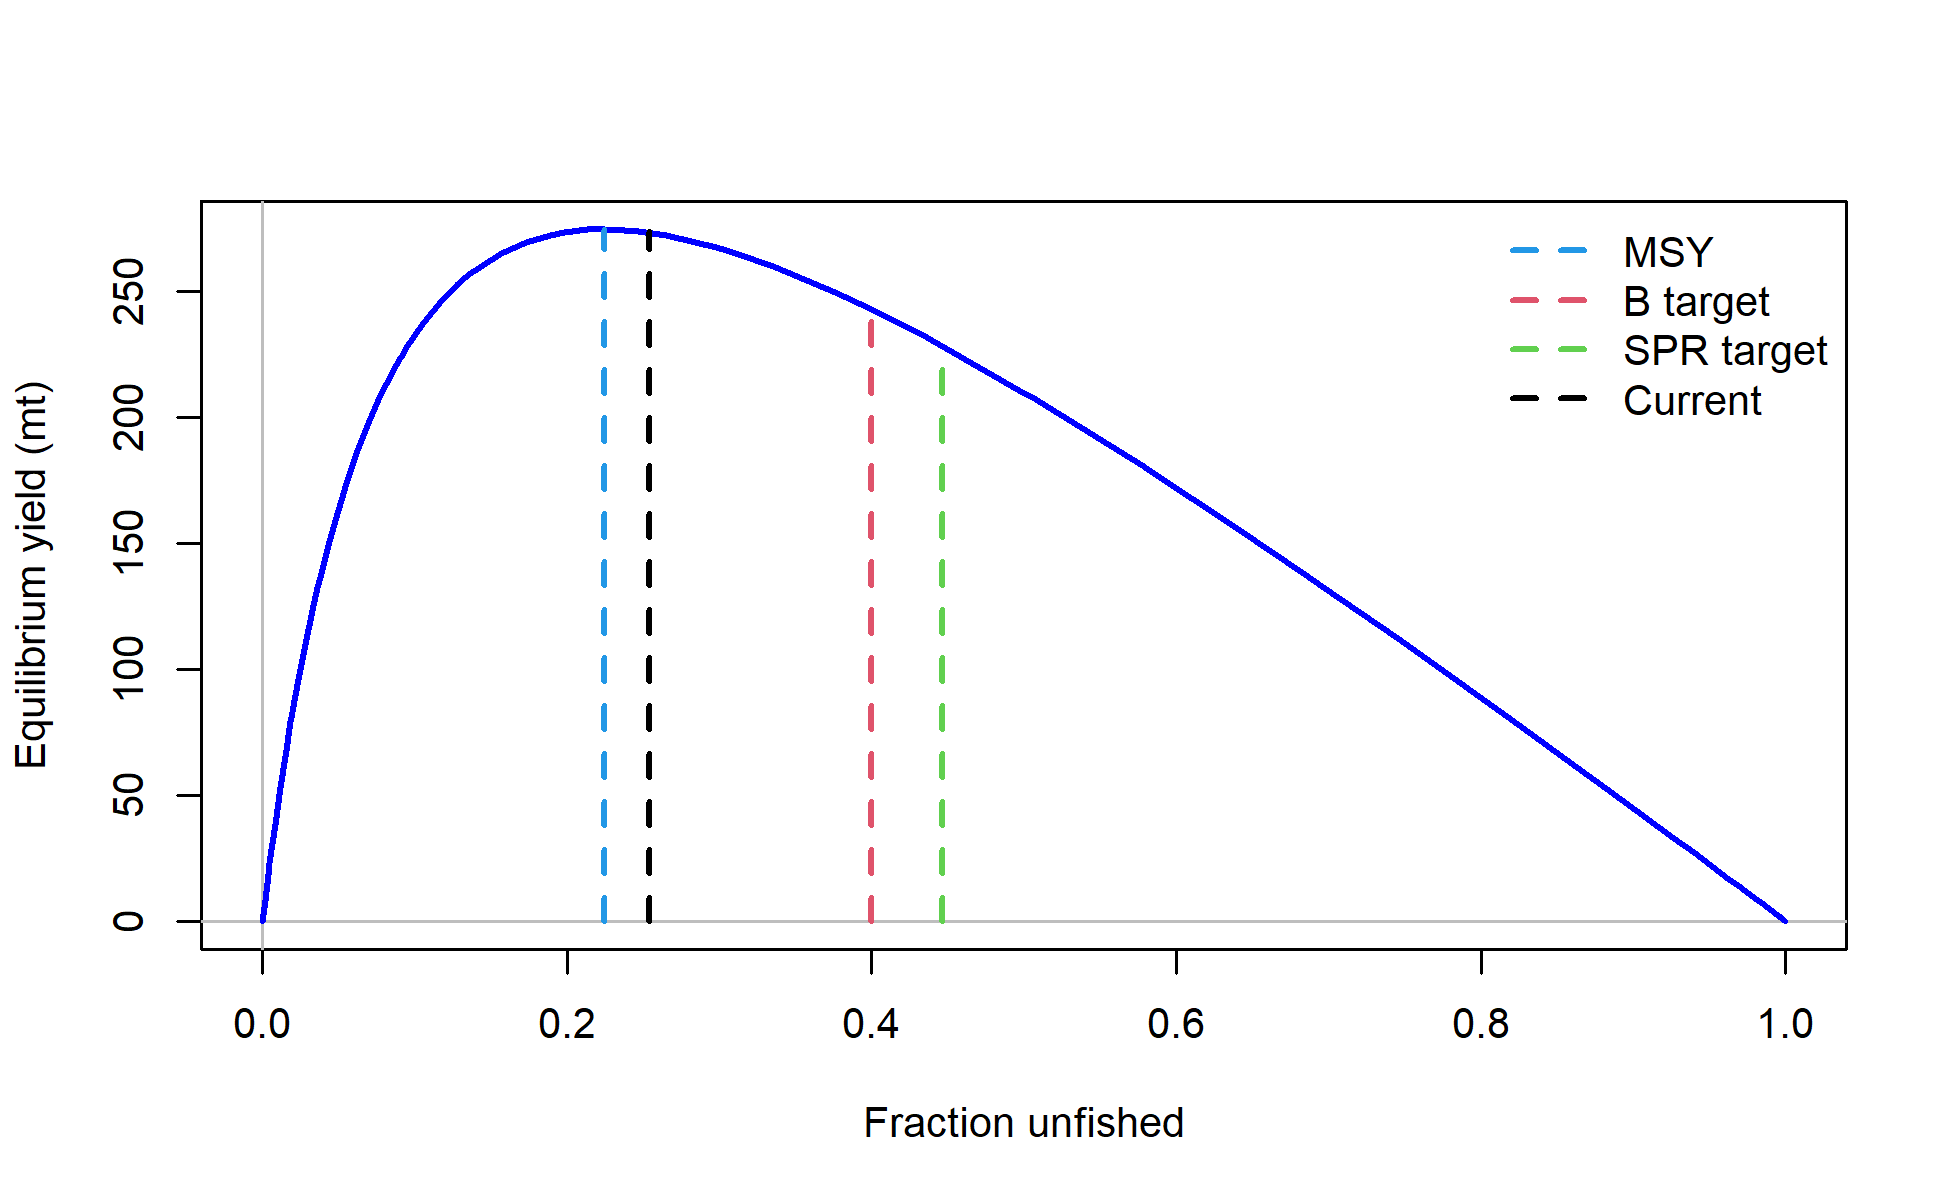
\includegraphics[width=1\textwidth,height=1\textheight]{C:/Users/Jason.Cope/Documents/Github/Sebastes_melanops_WA/Document/models/Reference model/plots/yield2_yield_curve_with_refpoints.png}
\caption{Equilibrium yield curve for the base case model. Values are based on (the time invariant) fishery selectivities and with steepness fixed at 0.72.\label{fig:es-yield}}
\end{figure}

\clearpage

\hypertarget{management-performance}{%
\subsection*{Management performance}\label{management-performance}}
\addcontentsline{toc}{subsection}{Management performance}

Black Rockfish removals have been below the equivalent Annual Catch Limit (ACL) over the recent decade (Table \ref{tab:manageES}). The ACL declined in 2017 relative to earlier years based on the 2015 assessment of Black Rockfish (Cope et al. 2016). In the last ten years, catches peaked in 2016 at 369 mt. Since then catches have declined to a recent low of 130 mt in 2020 with the catches in the final two model years remaining low with 197 mt in 2021 and 166 mt in 2022.

\begingroup\fontsize{10}{12}\selectfont
\begingroup\fontsize{10}{12}\selectfont

\begin{longtable}[t]{r>{\centering\arraybackslash}p{2.2cm}>{\centering\arraybackslash}p{2.2cm}>{\centering\arraybackslash}p{2.2cm}>{\centering\arraybackslash}p{2.2cm}}
\caption{\label{tab:manageES}Recent trend in the overfishing limits (OFL), the acceptable biological catches (ABCs),
                the annual catch limits (ACLs), and the total catch (mt).}\\
\toprule
Year & OFL & ABC & ACL & Catch\\
\midrule
\endfirsthead
\caption[]{Recent trend in the overfishing limits (OFL), the acceptable biological catches (ABC \textit{(continued)}}\\
\toprule
Year & OFL & ABC & ACL & Catch\\
\midrule
\endhead

\endfoot
\bottomrule
\endlastfoot
2013 & 430 & 411 & 411 & 326.02\\
2014 & 428 & 409 & 409 & 356.96\\
2015 & 421 & 402 & 402 & 363.44\\
2016 & 423 & 404 & 404 & 369.39\\
2017 & 319 & 305 & 305 & 241.02\\
2018 & 315 & 301 & 301 & 264.79\\
2019 & 312 & 298 & 298 & 251.09\\
2020 & 311 & 297 & 297 & 130.36\\
2021 & 319 & 293 & 293 & 197.68\\
2022 & 319 & 291 & 291 & 166.05\\*
\end{longtable}
\endgroup{}
\endgroup{}


\clearpage

\hypertarget{unresolved-problems-and-major-uncertainties}{%
\subsection*{Unresolved problems and major uncertainties}\label{unresolved-problems-and-major-uncertainties}}
\addcontentsline{toc}{subsection}{Unresolved problems and major uncertainties}

The biggest uncertainty is in the life history values, especially longevity and natural mortality. Lack of contrast in the biological data, despite generous sample sizes, can also make interpreting the population dynamics difficult, though current stock status does seem to be robust to this data.

\hypertarget{scientific-uncertainty}{%
\subsection*{Scientific uncertainty}\label{scientific-uncertainty}}
\addcontentsline{toc}{subsection}{Scientific uncertainty}

The model-estimated uncertainty around the 2023 spawning biomass was \(\sigma\) = 0.2 and the uncertainty around the OFL was \(\sigma\) = 0.19. This is likely underestimate of overall uncertainty because of the necessity to fix some life history parameters such as natural mortality and steepness, as well as a lack of explicit incorporation of model structural uncertainty. The alternative states of nature used to bracket uncertainty in the decision table assist with encapsulating model structure uncertainty.

\hypertarget{harvest-projections-and-decision-table}{%
\subsection*{Harvest Projections and Decision Table}\label{harvest-projections-and-decision-table}}
\addcontentsline{toc}{subsection}{Harvest Projections and Decision Table}

The following text will be modified, as appropriate, after the STAR panel and SSC meeting.

The Black Rockfish assessment is being considered as a category 1 assessment with a \(P^*\) = 0.45, \(\sigma\) = 0.50, and a time-varying buffer applied to set the ABC below the OFL. These multipliers are also combined with the rockfish MSY proxy of SPR\textsubscript{50} and the 40-10 harvest control rule to calculate OFLs and ACLs. A twelve year (2023-2034) projection of the reference model using these specifications along with input removals for 2023 and 2024 provided by the Groundfish Management Team (Katie Pierson, ODFW, pers. comm.) is provided in Table \ref{tab:projectionES}.

\begingroup\fontsize{10}{12}\selectfont
\begingroup\fontsize{10}{12}\selectfont

\begin{longtable}[t]{r>{\centering\arraybackslash}p{1.83cm}>{\centering\arraybackslash}p{1.83cm}>{\centering\arraybackslash}p{1.83cm}>{\centering\arraybackslash}p{1.83cm}>{\centering\arraybackslash}p{1.83cm}}
\caption{\label{tab:projectionES}Projections of potential OFLs (mt), ABCs (mt), estimated spawning output, and fraction unfished.}\\
\toprule
Year & Predicted OFL (mt) & ABC Catch (mt) & Age 0+ Biomass (mt) & Spawning Output & Fraction Unfished\\
\midrule
\endfirsthead
\caption[]{Projections of potential OFLs (mt), ABCs (mt), estimated spawning output, and fraction unfished. \textit{(continued)}}\\
\toprule
Year & Predicted OFL (mt) & ABC Catch (mt) & Age 0+ Biomass (mt) & Spawning Output & Fraction Unfished\\
\midrule
\endhead

\endfoot
\bottomrule
\endlastfoot
2023 & 275.48 & 252.31 & 5430.21 & 440.04 & 0.46\\
2024 & 268.96 & 246.34 & 5439.23 & 434.98 & 0.46\\
2025 & 264.55 & 242.29 & 5463.94 & 426.63 & 0.45\\
2026 & 262.69 & 240.58 & 5499.40 & 418.49 & 0.44\\
2027 & 263.00 & 240.85 & 5540.34 & 412.69 & 0.43\\
2028 & 264.77 & 242.47 & 5582.32 & 409.90 & 0.43\\
2029 & 267.34 & 244.82 & 5622.26 & 409.84 & 0.43\\
2030 & 270.19 & 247.42 & 5658.40 & 411.80 & 0.43\\
2031 & 272.95 & 249.95 & 5690.04 & 415.00 & 0.44\\
2032 & 275.42 & 252.21 & 5717.21 & 418.77 & 0.44\\
2033 & 277.51 & 254.13 & 5740.36 & 422.58 & 0.44\\
2034 & 279.22 & 255.70 & 5760.13 & 426.13 & 0.45\\*
\end{longtable}
\endgroup{}
\endgroup{}


Uncertainty in management quantities for the reference model was characterized by exploring various model specifications in a decision table. Initial explorations are considering alternative specifications of natural mortality and population scale. The resultant decision table will be provided in Table \ref{tab:es-dec-tab}.

Further details about selecting the decision table states of nature will be added here after the STAR panel.

\clearpage

\begingroup\fontsize{9}{11}\selectfont
\begingroup\fontsize{9}{11}\selectfont

\begin{longtable}[t]{l>{\raggedright\arraybackslash}p{0.08\linewidth}>{\raggedright\arraybackslash}p{0.08\linewidth}>{\raggedright\arraybackslash}p{0.1\linewidth}>{\raggedright\arraybackslash}p{0.09\linewidth}>{\raggedright\arraybackslash}p{0.1\linewidth}>{\raggedright\arraybackslash}p{0.09\linewidth}>{\raggedright\arraybackslash}p{0.1\linewidth}>{\raggedright\arraybackslash}p{0.09\linewidth}}
\caption{\label{tab:es-dec-tab}Decision table summary of 10 year projections beginning in 2023 for alternative states of nature based on an axis of uncertainty related to model structure relative to the reference model. Columns range over low (12.5 quantile), mid (reference model), and high states (87.5 quantile) of nature and rows range over different catch level assumptions. The first two years are fixed by the current harvest specifications.}\\
\toprule
\multicolumn{3}{c}{ } & \multicolumn{2}c{low $lnR_0$} & \multicolumn{2}c{Reference Model} & \multicolumn{2}c{High $lnR_0$} \\
\cmidrule(l{3pt}r{3pt}){4-5} \cmidrule(l{3pt}r{3pt}){6-7} \cmidrule(l{3pt}r{3pt}){8-9}
  & Year & Catch & Spawning Output & Fraction Unfished & Spawning Output & Fraction Unfished & Spawning Output & Fraction Unfished\\
\hline
&	2023	&	201	&	352	&	0.39	&	426	&	0.45	&	557	&	0.56\\	
&	2024	&	201	&	348	&	0.39	&	427	&	0.45	&	562	&	0.56\\	
&	2025	&	228	&	343	&	0.38	&	423	&	0.45	&	562	&	0.56\\	
&	2026	&	225	&	335	&	0.37	&	416	&	0.44	&	554	&	0.55\\	
&	2027	&	224	&	331	&	0.37	&	412	&	0.44	&	548	&	0.55\\	
P*=0.4	&	2028	&	224	&	331	&	0.37	&	411	&	0.43	&	543	&	0.54\\	
sigma=0.5	&	2029	&	225	&	33	&	0.37	&	412	&	0.44	&	541	&	0.54\\	
&	2030	&	226	&	340	&	0.38	&	416	&	0.44	&	540	&	0.54\\	
&	2031	&	227	&	346	&	0.39	&	421	&	0.45	&	541	&	0.54\\	
&	2032	&	228	&	354	&	0.39	&	427	&	0.45	&	543	&	0.54\\	
&	2033	&	228	&	361	&	0.40	&	433	&	0.46	&	546	&	0.54\\	
&	2034	&	226	&	368	&	0.41	&	439	&	0.48	&	548	&	0.55\\	
\hline																	
	&	2023	&	201	&	352	&	0.39	&	426	&	0.45	&	557	&	0.56\\	
	&	2024	&	201	&	348	&	0.39	&	427	&	0.45	&	562	&	0.56\\	
	&	2025	&	245	&	343	&	0.38	&	423	&	0.45	&	562	&	0.56\\	
	&	2026	&	241	&	333	&	0.37	&	414	&	0.44	&	552	&	0.55\\	
	&	2027	&	240	&	326	&	0.36	&	407	&	0.43	&	543	&	0.54\\	
P*=0.45	&	2028	&	241	&	325	&	0.36	&	404	&	0.43	&	537	&	0.54\\	
sigma=0.5	&	2029	&	242	&	326	&	0.36	&	404	&	0.43	&	532	&	0.53\\	
	&	2030	&	244	&	330	&	0.37	&	406	&	0.43	&	530	&	0.53\\	
	&	2031	&	245	&	335	&	0.37	&	410	&	0.43	&	529	&	0.53\\	
	&	2032	&	246	&	341	&	0.38	&	414	&	0.44	&	529	&	0.53\\	
	&	2033	&	247	&	347	&	0.39	&	418	&	0.44	&	530	&	0.53\\	
	&	2034	&	248	&	352	&	0.39	&	423	&	0.45	&	531	&	0.53\\	
\hline																	
	&	2023	&	201	&	352	&	0.39	&	426	&	0.45	&	557	&	0.56\\	
	&	2024	&	201	&	348	&	0.39	&	427	&	0.45	&	562	&	0.56\\	
	&	2025	&	279	&	343	&	0.38	&	423	&	0.45	&	562	&	0.56\\	
	&	2026	&	279	&	328	&	0.36	&	409	&	0.43	&	547	&	0.55\\	
Equilibrium	&	2027	&	279	&	317	&	0.35	&	398	&	0.42	&	533	&	0.53\\	
yield	from	&	2028	&	279	&	311	&	0.35	&	390	&	0.41	&	522	&	0.52\\
FMSY	proxy	&	2029	&	279	&	308	&	0.34	&	386	&	0.41	&	513	&	0.51\\
of	SPR=0.5	&	2030	&	279	&	309	&	0.34	&	384	&	0.41	&	507	&	0.50\\
	&	2031	&	279	&	311	&	0.35	&	384	&	0.41	&	502	&	0.50\\	
	&	2032	&	279	&	314	&	0.35	&	386	&	0.41	&	500	&	0.50\\	
	&	2033	&	279	&	317	&	0.35	&	388	&	0.41	&	498	&	0.50\\	
	&	2034	&	279	&	320	&	0.36	&	390	&	0.41	&	497	&	0.50\\*	
\hline
\end{longtable}
\endgroup{}
\endgroup{}


\clearpage

\hypertarget{research-and-data-needs}{%
\subsection*{Research and data needs}\label{research-and-data-needs}}
\addcontentsline{toc}{subsection}{Research and data needs}

Recommended avenues for research to help improve future Black Rockfish stock assessments:

\begin{enumerate}
\def\labelenumi{\arabic{enumi}.}
\tightlist
\item
  Continue to develop the nearshore fishery-independent survey, as the other available surveys provide week information for the trend in the population.
\item
  Improve understanding of broader ecosystem considerations within the context of Black Rockfish (and other nearshore species) management. Evaluate and develop linkages between Black Rockfish population dynamics and environmental, oceanographic, and climate variables. In particular, develop multi-scale models (e.g., species distribution models) that can evaluate spatial patterns (e.g., multi-use areas or closures to fishing) and climate impacts (e.g., growth or distribution shifts) for vulnerable nearshore species. Utilize the growing body of ecosystem information available for the California Current Large Marine Ecosystem, as exemplified in the PFMC IEA report.
\item
  Continue work on the investigation into the movement, behavior or mortality of older (\textgreater{} age 10) females to further reconcile their absence in fisheries data. In particular, conduct genetics studies on fish observed off of the continental shelf (middle of the gyre and at sea mounts) to determine their association with the nearshore stocks.
\item
  Continue to build evidence for appropriate natural mortality values for females and males. This will help resolve the extent to which dome-shaped age-based selectivity may be occurring for each.
\item
  Design and conduct research studies to better understand the trade-offs revealed in this assessment between Black Rockfish biology and population scale that seem be at odds. If discrepancies can not be uncovered, evaluate management procedures that are as robust as can be to this trade-off.
\item
  Conduct early life history studies that provide a better understanding of the ecology and habitats of Black Rockfish from settlement to age-1.
\end{enumerate}

\vspace{500cm}

\pagebreak
\setlength{\parskip}{5mm plus1mm minus1mm}
\pagenumbering{arabic}
\setcounter{page}{1}
\renewcommand{\thefigure}{\arabic{figure}}
\renewcommand{\thetable}{\arabic{table}}
\setcounter{table}{0}
\setcounter{figure}{0}

\hypertarget{introduction}{%
\section{Introduction}\label{introduction}}

This assessment report describes the stock of Black Rockfish (\emph{Sebastes melanops}) off the Washington coast in U.S. waters, using data through 2022. The stocks of Black Rockfish in Washington, Oregon, and California waters are each modeled as separate stocks with the population estimates reported in stock-specific assessment reports (Figure \ref{fig:map}). This assessment does not account for populations located in Canadian waters or other areas off the U.S. West Coast and assumes that these southern and northern populations do not contribute to nor take from the population being assessed here.

\hypertarget{basic-information}{%
\subsection{Basic Information}\label{basic-information}}

Black Rockfish are an important component of the recreational fisheries in the nearshore waters off central and northern California, Oregon, and Washington, as well as the non-trawl commercial fisheries in California and Oregon. They range as far north as Amchitka and Kodiak islands in Alaska and are considered uncommon south of central California (Love et al. 2002).

Previous assessments of Black Rockfish off Washington (Wallace et al. 1999; Wallace and Tsou 2007) describe a study of coastal Black Rockfish genetic structure using 10 sampled sites collected from northern California to southern British Columbia between 1995-97. Results of that study support the notion of separate genetic stocks north and south of Cape Falcon. However, a later study (Baker 1999) of Black Rockfish collected from eight sites along the northern Oregon coast concluded that Black Rockfish from north and south of Cape Falcon were genetically very similar.

A stock boundary line at the Columbia River seems reasonable for Black Rockfish, both because it is a state fishery management boundary and because the Columbia River plume is likely to be a natural barrier to the north-south exchange of Black Rockfish adults and larvae. Given the spatial resolution of the historical commercial fishery data, it is very problematic to estimate the catch of Black Rockfish taken north of Cape Falcon but south of the Columbia River.

During a preliminary workshop in April 2015 (Council 2015), it was agreed that the assessments for nearshore species should at a minimum be spatially stratified with boundaries at the California/Oregon border (\(42^\circ\) N. latitude) and the OR/WA border (\(46^\circ 16^\prime\) N. latitude). Such a spatial stratification would be consistent with two ideas: (a) these nearshore species do not exhibit much adult movement and (b) exploitation and management histories have varied significantly among the three states. Together these features would likely create appreciable state-to-state differences in age composition for each of the three species.

At the same nearshore stock assessment workshop, it was agreed that recreational catch histories for the stocks of Black Rockfish should be assembled on the basis of port of landing rather than location of fish capture, even though fishing vessels landing their catches into a port in one state might have captured fish in waters off a neighboring state.

Accounting for location of capture is very problematic for recreationally caught fish and for commercial catches taken with non-trawl types of gear (e.g., hook-and-line), for which there are no or very limited logbooks that report fishing location. For these regional assessments the commercially caught Black Rockfish were apportioned to assessment region based on the port of landing, with the exception of trawl caught fish landed into Astoria, OR. Most of these fish were assumed to have been caught off Washington and most of the trawl landings into Astoria were therefore included with the catch history for the Washington assessment region. Additional details are provided in the commercial landings section \ref{com-landings}.

\hypertarget{life-history}{%
\subsection{Life History}\label{life-history}}

Adults tend to occur in schools over rocky structure at depths less than 40 fathoms, and sometimes feed actively on or near the surface. They feed on a wide variety of prey including zooplankton, krill, mysids, sand lance, and juvenile rockfish, and are subject to predation by lingcod and marine mammals (Love et al. 2002).

Although tagging studies have documented some individuals moving long distances (several hundreds of miles), the vast majority of recaptured individuals were found close to the areas of initial capture and tagging (Culver 1987; Ayres 1988; Starr and Green 2007; Wallace et al. 2010). Results from a 2004-05 study off Newport, Oregon of 42 Black Rockfish implanted with acoustic tags indicated that all but seven fish remained within range of a 3 x 5 km array of acoustic receivers during one full year of monitoring and had relatively small home ranges that did not vary seasonally (Parker et al. 1995). Green and Starr (2011) report similar findings from a study in Carmel Bay, California of 23 acoustically tagged Black Rockfish. The extensive Washington state tagging study also supported low movements for most individuals, with some exceptional movements recorded (Wallace et al. 2010).

Like all members of the genus Sebastes, Black Rockfish have internal fertilization and bear live young approximately two months after insemination. Black Rockfish are quite fecund, with a six-year-old female annually producing about 300,000 embryos and a 16-year-old producing about 950,000 embryos (Bobko and Berkeley 2004a). Recent studies have demonstrated that the relative number and quality of larvae increase with age in female Black Rockfish (Berkeley et al. 2004; Hixon et al. 2014a). Parturition of larvae occurs during winter (Echeverria 1987) and larvae and small juveniles are pelagic for several months to a year (Boehlert and Yoklavich 1983). Settlement occurs in estuaries, tide-pools, and in the nearshore at depths less than 20 m (Stein and Hassler 1989).

Black Rockfish begin recruiting to nearshore fisheries at 3-4 years of age, corresponding to a fork length of about 25-30 cm, and 50\% of females attain maturity between 6-8 years of age, corresponding to a fork length of about 38-42 cm. Adult female Black Rockfish grow 3-5 cm larger than males, with a few females attaining fork lengths greater than 55 cm.

\hypertarget{ecosystem-considerations-1}{%
\subsection{Ecosystem Considerations}\label{ecosystem-considerations-1}}

No formal ecosystem considerations have been made given the lack of data for such an undertaking. Differences in growth though time have been considered in the model specification in the Washington model. Though the mechanism is not specified, this could certainly be due to process error driven by environmental conditions.

\hypertarget{historical-and-current-fishery-information}{%
\subsection{Historical and Current Fishery Information}\label{historical-and-current-fishery-information}}

Black Rockfish are harvested by a wide variety of fishing methods including trawling, trolling, and hook-and-line fishing with jigs and long-lines since at least the 1940s. Although Black Rockfish have never been a dominant component of any commercial fisheries, they have been important incidental catch in the troll fishery for salmon and the troll and jig fisheries for groundfish. With the decline of salmon fishing opportunities in the late 1970s and early 1980s Black Rockfish became a vital target of marine recreational fisheries in Oregon and Washington, especially during periods of restricted or slack fishing for salmon, halibut, and tuna.

Since 1990 annual recreational harvests of Black Rockfish have averaged 272.5 tons off Washington. Commercial annual harvests by non-trawl gear types during the same period averaged 14.7 tons in Washington. Harvests by trawl on average during this period have been very low (Table \ref{tab:total_removals}).

\hypertarget{summary-of-management-history-and-performance}{%
\subsection{Summary of Management History and Performance}\label{summary-of-management-history-and-performance}}

Regulation of the Black Rockfish fisheries by the PFMC prior to 2004 was accomplished primarily by trip limits for commercial fisheries and bag limit restrictions for recreational fisheries, with different limits applying in different geographic regions (see Table 1 in Ralston and Dick (2003)). Some other important regulations include the following:

\begin{itemize}
\tightlist
\item
  1995: The commercial hook-and-line fishing in Washington state waters (0-3 miles) was closed to preserve recreational fishing opportunities and avoid localized depletion; the closure was extended to trawlers in 1999.\\
\item
  2003: The Pacific Fishery Management Council (PFMC) established Rockfish Conservation Areas (RCAs) to control catches of overfished rockfish species, and large portions of the shelf were closed to fishing. Differential trip limits were applied north and south of a management boundary at \(40^\circ 10^\prime\) N. latitude for nearshore Sebastes species.
\item
  In 2008 the groundfish trawl fishery was closed in Washington from the seaward RCA boundary to the shore north of \(48^\circ 10^\prime\) N. latitude to address increased encounters with Yelloweye Rockfish and Canary Rockfish.
\end{itemize}

In recent years regulations for the marine sport fisheries, which has been the major source of mortality on Black Rockfish, have become quite complicated and variable through time. Tools for regulating the sport fishery include closed areas, depth restrictions, seasonal closures, and bag limits.

Washington had a recreational daily bag limit for rockfish (all species) of 15 fish per day from 1961 to 1991, 12 fish per day from 1992 to 1994, 10 fish per day from 1995 to 2016, and 7 fish per day from 2017 to 2022. The bag limit for Blue Rockfish plus Black Rockfish in Marine Area 4B (Neah Bay) has been 6 fish per day since 2010. Fishing seasons for groundfish species are structured to provide year-round fishing opportunities, if possible. Depth restrictions vary by state management area, being more restrictive in the north compared to the south due to higher encounter rates with overfished Yelloweye Rockfish and Canary Rockfish (declared rebuilt in 2015). There is no minimum size limit for Black Rockfish.

\hypertarget{canadian-and-alaska-fisheries}{%
\subsection{Canadian and Alaska fisheries}\label{canadian-and-alaska-fisheries}}

Black Rockfish is a ``Non-Quota'' species in the Department of Fisheries and Oceans╔ Management Plan, and is not formally assessed in nearshore Canada waters (Fisheries and Canada 2014).

Alaska has initiated stock assessments for Black Rockfish throughout the state. These efforts are ongoing.

\hypertarget{data-and-model-inputs}{%
\section{Data and Model Inputs}\label{data-and-model-inputs}}

Data from a wide range of programs were available for possible inclusion in the current assessment model. Descriptions of each data source included in the model (Figure \ref{fig:data-plot}) and sources that were explored but not included in the base model are provided below. Data that were excluded from the base model were excluded only after being explicitly explored during the development of this stock assessment and found to be inappropriate for use or had not changed since their past exploration for previous Black Rockfish stock assessments when they were not used.

\hypertarget{fishery-dependent-data}{%
\subsection{Fishery-Dependent Data}\label{fishery-dependent-data}}

The following subsections describe the removal histories for each fleet. Some assumptions about historical removals were revisited and changed from the last assessment. Comparisons of total fishery removals in the current and previous assessments are shown in (Figure \ref{fig:catch-ts-comparison}).

\hypertarget{commercial-removals}{%
\subsubsection{Commercial Removals}\label{commercial-removals}}

\hypertarget{com-landings}{%
\paragraph{Landings}\label{com-landings}}

The systems along the U.S. West Coast for monitoring commercial fishery landings in the past did not keep track of the landings of individual rockfish species, largely because many rockfish species have similar market characteristics and therefore were landed as an unsorted mix of species. Black Rockfish in particular, which are a nearshore species and much less abundant than many of the offshore rockfish species, were generally landed in mixed-species categories and were not required to be sorted into its own market category until 2006. As a consequence, the historical records do not provide a detailed accounting of the landings of Black Rockfish. The basic approach taken to develop the landings series in this assessment (as in past assessments) was to apply values for the proportion of Black Rockfish sampled in mixed-rockfish landings. Data on the proportions of Black Rockfish are sparse, with the consequence that the landings reconstructions are highly uncertain.

Since 1935, commercial fishing vessels have been required to submit a fish receiving ticket (``fish ticket'') for each landing. Rockfish landings from domestic fishers are usually reported in mixed-species market categories, but were not routinely sampled for species composition by port samplers until 2000. The information required on the fish ticket and sampling methods have changed through time. A historical catch reconstruction for Black Rockfish was conducted for the 2015 stock assessment of Black Rockfish (Cope et al. 2016). We keep the same catch history and updated the total removal time series through 2022 (Table \ref{tab:total_removals}).

It has been and continues to be a common practice for Oregon fleets to fish off the Washington coast and land their catches in Oregon ports. Although the separate geographic assessments by state region would ideally have strict geographic separation of landed catch to the location of capture, this is not possible to accomplish because information on the fishing location is generally unavailable. Beginning in 2004, Oregon required a logbook for commercial vessels participating in its nearshore fishery. To account for the Black Rockfish removed from Washington water by Oregon fleets historically, staff from the Oregon Department of Fish and Wildlife (ODFW) used species composition samples collected during 1976 to 1993 to conduct an analysis of the spatial distribution of Black Rockfish landed at Astoria, OR. Astoria is the northernmost port in Oregon and is located near the mouth of the Columbia River, which forms the boundary between Oregon and Washington. The portion of aggregated rockfish landed pounds that were taken north of the Columbia River (i.e., from waters off Washington) was 98.6\%. This percentage was applied to all historical trawl landings of rockfish at Oregon's Columbia River District ports prior to 1976. Of the 98.6\% of aggregated rockfish landings, it was assumed 14.1\% was Black Rockfish in the 2015 assessment (Cope et al. 2016). This percentage is much higher than the values used for the Washington catch reconstruction. Therefore, we recalculated this portion by using Washington's historical species composition data which is not available in Pacific Fisheries Information Network (PacFIN) for pre-1981 and data available in PacFIN for 1981 to 1986. The revised proportions of Black Rockfish in the aggregated rockfish trawl landings are 3\% and 4\% for pre-1981 and 1981-1986, respectively. Non-trawl landings into Astoria were assumed to have been caught from Oregon waters, which is the same assumption used in the 2015 assessment.

Starting in 1994 Black Rockfish landed into Oregon were legally required to be sorted and sold in a separate Black Rockfish market category and were also reported as separate retained catches in the mandatory trawl logbooks. Based on the retained catches reported in the logbooks, the estimated proportion of the trawl-caught Black Rockfish that were caught from off Washington and landed into Astoria ranged from 65 to 100\%. These Black Rockfish are accounted for in the Washington regional assessment (Table \ref{tab:rec_catch_reconstruction}).

The Washington Department of Fish and Wildlife (WDFW) provided commercial fishery landings based on fish ticket records of Black Rockfish harvested off Oregon by vessels landing at ports in Washington. Landings were less than 1 mt per year for the period of 1971 to 2014; therefore, all landings to Washington ports were assumed to occur in waters off Washington in this assessment.

\hypertarget{foreign-fishery-removals-of-black-rockfish}{%
\paragraph{Foreign Fishery Removals of Black Rockfish}\label{foreign-fishery-removals-of-black-rockfish}}

Rogers (2003) developed catch reconstructions for removals by foreign trawlers operating off the U.S. West Coast during the late 1960s to mid-1970s. Although this study reports that Japanese vessels operating in the Columbia and Eureka statistical areas (Oregon and northern California) caught substantial amounts of Black Rockfish, with cumulative catches of more than 500 mt over 10 years, it seems very unlikely that foreign vessels could have operated sufficiently close to shore to catch appreciable amounts of Black Rockfish. This assessment does not include Rogers' (2003) estimates of foreign fleet removals of Black Rockfish.

\hypertarget{recreational-removals}{%
\subsubsection{Recreational Removals}\label{recreational-removals}}

The Washington recreational catch history of Black Rockfish was reconstructed using several direct and indirect records of Black Rockfish catch (Table \ref{tab:rec_catch_reconstruction}). All primary sources report catch in numbers of fish. As sources have been modified and re-evaluated, a completely new catch reconstruction for Washington was developed for 2015 assessment. This catch history was updated to include 2015-2022 estimates in this assessment.

\hypertarget{estimated-discards}{%
\subsubsection{Estimated Discards}\label{estimated-discards}}

In the previous assessment, commercial discards were not accounted for due to the information provided by the West Coast Groundfish Observer Program (WCGOP) at that time, showing about a 1\% discard rate in their survey. We evaluated the WCGOP estimates of Black Rockfish discards from 2002-2013, which showed a total of 32.2 mt in estimated discards and total landings of 2,042.5 mt coastwide, resulting in a rough discard rate estimate of 1.58\%.

Recreational discard estimates were not available until 2002. Numbers of discarded-by-depth Black Rockfish were estimated using the same catch expansion algorithm for landed catch. Surface release mortalities adopted by the Groundfish Management Team (GMT) in their death-by-depth matrix (11\%, 20\%, 29\%, and 63\%) were then applied to the number of released Black Rockfish for each of 4 release depth bins (0-10 fm, 11-20 fm, 21-30 fm, and \textgreater30fm), respectively. Total dead released Black Rockfish were then summed across each depth bin. The average weights of discards were assumed to be the same as the average weights of landed and multiplied by the number of released dead to get total dead in metric tons. For pre-2002 release, proportions of releases based on a ratio estimator using 2003-2007 data were applied. The same algorithm used for splitting retained catch was applied for the split between charter and private vessels. The overall average discard rate in the recreational fisheries was 1.37\%. There was no information on Washington commercial discards, so the rate of 1.37\% (same as the historical recreational discards) was also applied to the entire commercial time series. This low rate was similar to discard rates estimated in the other states. Annual retained and discarded catches are summarized in (Table \ref{tab:annual_discards}).

\hypertarget{composition-data}{%
\subsection{Composition Data}\label{composition-data}}

Fish length measurements, primarily from the recreational fishery, are one of the major sources of data for this assessment (Figure \ref{fig:data-plot}).

\hypertarget{length-and-age-sample-sizes}{%
\subsubsection{Length and Age Sample Sizes}\label{length-and-age-sample-sizes}}

The level of commercial fishery sampling, trawl and non-trawl, for Black Rockfish has been erratic, with limited sample sizes for length and ages taken in Washington until the early 1990s. The primarily source of fishery-dependent length and age data for Black Rockfish arise from the recreational fishery.

\hypertarget{multinomial-sample-sizes}{%
\paragraph{Multinomial Sample Sizes}\label{multinomial-sample-sizes}}

Initial input values for the multinomial samples sizes determine the relative weights applied in fitting the annual composition data within the set of observations for each fishing fleet in the model. The initial input values in this assessment were based on the following equation developed by I. Stewart and S. Miller (NWFSC), and presented at the 2006 Stock Assessment Data and Modeling workshop. The input sample sizes for all commercial data were calculated based on a combination of trips and fish sampled:

\begin{centering}

Input effN = $N_{\text{trips}} + 0.138 * N_{\text{fish}}$ if $N_{\text{fish}}/N_{\text{trips}}$ is $<$ 44

Input effN = $7.06 * N_{\text{trips}}$ if $N_{\text{fish}}/N_{\text{trips}}$ is $\geq$ 44

\end{centering}

\hypertarget{length-compositions}{%
\subsubsection{Length Compositions}\label{length-compositions}}

The length data for the assessment model were tabulated into 2-cm length bins ranging from 10 cm to 64 cm, with accumulator bins at each end.

The length composition data indicate some general differences between the three fishery types, with the trawl fisheries producing the largest fish, the recreational fisheries producing the smallest fish, and the non-trawl fisheries producing fish of intermediate length (Figures \ref{fig:trawl-length-comps}-\ref{fig:rec-length-comps}), though the difference between the last two are not large. There is little evidence in any of the length composition data of distinct modes or successions of modes from one year to the next that might represent strong year-classes.

\hypertarget{commercial}{%
\subparagraph{Commercial}\label{commercial}}

Biological data for the commercial fishery were extracted from PacFIN on 23 March, 2023. These data are from trawl and non-trawl (hook-and-line) fisheries (there has been no live-fish fishery off Washington). Of the 8,807 records available within PacFIN (each representing a single specimen), 4,990 were from the commercial trawl fishery (Table \ref{tab:WA_Comm_Lt_samps}).

For use as compositional data in the assessment, lengths undergo a two-stage expansion as implemented in the \href{https://github.com/pfmc-assessments/PacFIN.Utilities}{PacFIN.Utilities R library}. The expansions are by weight, catch/sampled catch; first on a per-trip level, and then on a per-year, per-fishery level. Expansion factors have a minimum value of 1, and are capped at their 90th percentile value. The final sample size is the product of the two expansion factors, which is then capped at its 90th percentile value.

The data were stratified by fishery and sex (Table \ref{tab:WA_Comm_Lt_samps}). The final sample sizes were stratified and summed by length bin (10 cm to 64 cm bins, 2 cm in width), and an effective sample size is computed from the number of trips and number of fish each stratum represents, according to the Stewart and Miller method for multinomial fishery data.

\hypertarget{recreational}{%
\subparagraph{Recreational}\label{recreational}}

The WDFW biological database provided sampled length data from the recreational fishery for sexed and unsexed samples for years 1979-2022. Sexed samples were the largest sample sizes and covered most years (Table \ref{tab:rec_length_sample}). Composition data were used as collected (i.e., not expanded). Effective sample sizes were based on unique ``sequence'' sizes, which is roughly equivalent to a trip.

\hypertarget{survey-data}{%
\paragraph{Survey data}\label{survey-data}}

The WDFW provided sampled length data from the tagging survey for sexed and unsexed samples for years 1981-2022. Samples from 1998-2018 were used in the analysis for the indices (Table \ref{tab:survey_sample_indices}). Unsexed and sexed data were generally available in different years. Like the recreational data, composition data were used as collected (i.e., not expanded) and effective sample sizes were based on unique ``sequence'' sizes, which is roughly equivalent to a trip.

\hypertarget{age-compositions}{%
\paragraph{Age Compositions}\label{age-compositions}}

Commercial age composition data were a subset of the length data, 7,863 records in total, and were expanded in the same manner as the lengths (Table \ref{tab:WA_Comm_Lt_samps}). Ages were stratified by fishery and sex (female, male and unsexed), and binned in 1-year bins from 0 to 40.

Samples were also available by sex for several years in the recreational data (Table \ref{tab:rec_age_sample}). Age samples are available by sex from 1980 until 2022 in the recreational data, and comprise the largest amount of age data in the model. Ages are binned in 1 year bins from 0 to 40 stratified by sex.

Conditional age-at-length compositions were not expanded, though marginal compositions were. For conditional age-at-length data the effective sample sizes were the sum of all individual age samples per length bin. Ages were modeled as conditional age-at-length, though marginal age compositions were included in the model with no contribution to the likelihood. This inclusion allows one to see how well the marginal age compositions are fit without having them effect overall model fit.

\hypertarget{abundance-indices}{%
\subsubsection{Abundance Indices}\label{abundance-indices}}

Indices of abundance can provide another source to inform the trend and dynamics of the population. Most assessments of U.S. West Coast groundfish stocks rely on estimates of relative stock biomass from research trawl surveys to provide information on biomass trends, but Black Rockfish are very infrequently caught in any of the bottom trawl surveys, which have a limited coverage of shallow nearshore waters (none of the surveys have ever been conducted in waters shallower than 55 m). Thus fishery-dependent catch-per-unit effort data are often considered as a source for tracking abundance. Below is a description of how recreational data was considered as an index for Black Rockfish.

\hypertarget{dockside-catch-per-unit-effort-for-washington}{%
\paragraph{Dockside Catch-Per-Unit-Effort for Washington}\label{dockside-catch-per-unit-effort-for-washington}}

WDFW's Ocean Sampling Program (OSP) collects data on catch and effort in the State's coastal recreational fisheries. This dockside data was considered for use as a fishery-dependent index of abundance for 1981-2022. OSP collects trip level data with key data fields including the number of landed fish by species or species category, the number of anglers, marine area fished, and trip and boat type. The number of released fish has only been recorded since 2003. Finer scale measures of effort, such as the amount of time fished by each angler, are not recorded.

Thes data were used to produce an index of abundance for the 2015 assessment of Black Rockfishusing the available years at the time. The analysts used the Stephens-MacCall method (Stephens and MacCall 2004) as an objective approach for identifying trips that visited Black Rockfish habitat. Black Rockfish were found to be extremely common in bottomfish catches, so the Stephens-MacCall filtering made little difference in the data sets. The index was standardized using a delta-GLM approach, where the catch occurrence (binomial) component was modeled using a logit link function and the positive catch component was modeled using either lognormal or gamma distributions.

For this assessment, the recreational dockside data in its entirety was re-evaluated to develop an index of abundance. However, changes in management measure enacted after the 2015 assessment led to further consideration of whether the data could provide a reliable signal on abundance. Black Rockfish are subject to a total rockfish bag limit in Washington but make up the bulk of the retained rockfish, especially in Marine Area 2 and increasingly so over time in Marine Areas 3 and 4 (Figure \ref{fig:blackrock_percentage}). Since 2003, the rockfish limit has been a subset of a total bag limit on bottomfish. After the bag limit decreased from 10 to 7 rockfish in 2017, there was a clear drop in Black Rockfish CPUE limit for both private and charter boats in most every marine area (Figure \ref{fig:baglimit_numbers}). With no finer scale measure of effort available, it is not possible to determine if there were changes in the fishing or search time needed to reach the bag limit. Trips may have spent less time fishing for Black Rockfish than in years when the bag limit was higher.

There were several bag limit changes over the time series prior to 2017. Further evaluation of the time series showed past periods where the bag limit was also reached on a high percentage of trips, especially for charter boats in Marine Area 2 (Figure \ref{fig:baglimit_percentage}). Daily rockfish limits were 15 fish from 1981-1991, 12 fish from 1992-1994 (except in area 1 where it remained at 15), and 10 fish from 1995-2016. The fishery has seen other management measure changes where the affect on the relationship between CPUE and abundance is difficult to determine. In 2003, management restricted summer fishing depths to shallower than 20-fathoms in WDFW marine areas 3 and 4, and in 2006 modified this depth restriction to 30-fathoms in marine areas 2, 3, and 4. And sub-bag limits for desirable species like Canary Rockfish have also changed and could affect fishing behavior for Black Rockfish. General bottomfish bag limit changes also occurred reducing retention of total bottomfish from no limit to 15 fish in 2002 and 12 fish in 2011.

In consideration of management changes and the potential for non-abundance related effects on CPUE, OSP dockside data was separated by fleet and filtered to create two indices, as described below. Sensitivity runs that excluded the OSP dockside data entirely were also considered.

\hypertarget{dockside-cpue-private-fleet-1981-2016}{%
\paragraph{Dockside CPUE Private Fleet 1981-2016}\label{dockside-cpue-private-fleet-1981-2016}}

Dockside data was filtered for interviews with private boats and several covariates including year, month, area, daily bag limits and depth restrictions were considered. Depth was not consistently recorded, so depth-based management could not be filtered out. Instead, covariates for depth restrictions and daily bag limits were included to represent management changes. To be certain that the characteristics of a ``trip'' were comparable, the analysis was restricted to bottomfish only trips, in areas specific to rockfish, for private boats from 1981 through 2016 (43,187 records). The truncation of the data series excluded the latest large bag limit restriction that took effect in 2017.

CPUE was calculated for each angler trip, where total catch was defined as the sum of all reported retained catch (in numbers) and total effort was defined by the number of anglers. CPUE was modeled using the same delta-GLM approach used in 2015. Lognormal (Figure \ref{fig:private-log-diags}) and gamma (Figure \ref{fig:private-gam-diags}) distributions for the positive catch component were considered, but diagnostics favored the choice of a lognormal distribution for the final index. The CPUE time series is shown in Figure \ref{fig:private-index}. A bootstrap analysis (N=500) was used to estimate the coefficient of variation of the year effects (\ref{fig:private-CVs}).

\hypertarget{dockside-cpue-charter-fleet-1981-1994}{%
\paragraph{Dockside CPUE Charter Fleet 1981-1994}\label{dockside-cpue-charter-fleet-1981-1994}}

For the charter boat fleet interview data collected from 1981 through 1994 was modeled as being less sensitive to the effects of bag limits. It was also a key period in the fishery where effort was ramping up. As with the private fleet analysis, data was restricted to bottomfish only trips in areas specific to rockfish, for charter boats from 1981 through 1994 (16,364 records).

Several covariates were considered in the full model including year, month, area, daily bag limit and depth restriction. As with private boats, depth was not consistently recorded and could not be used. A covariate for daily bag limits was included to represent management changes but depth restrictions did not go into effect until after this data time series and were not incorporated. AIC was not used to choose between error distributions for the positive catches. This was instead done using quantile-quantile plots (Figures \ref{fig:charter-log-diags} and \ref{fig:charter-gam-diags}). The full model with a gamma error distribution was chosen (Figure \ref{fig:charter-index} and a bootstrap analysis (N=500) was used to estimate the the coefficient of variation of the year effects (Figure \ref{fig:charter-CVs}).

\hypertarget{fishery-independent-data}{%
\subsection{Fishery-Independent Data}\label{fishery-independent-data}}

\hypertarget{abundance-indices-1}{%
\subsubsection{Abundance Indices}\label{abundance-indices-1}}

\hypertarget{tagging-and-nearshore-survey-cpue-for-washington}{%
\paragraph{Tagging and Nearshore Survey CPUE for Washington}\label{tagging-and-nearshore-survey-cpue-for-washington}}

Fishery-independent data available for this assessment came from two distinct WDFW research projects. The first was the Black Rockfish Tagging Program that was initiated in the early 1980s and provided CPUE of Black Rockfish captured for tag releases primarily off the central coast of Washington. The second data set was from the standardized Coastwide Rod-and-Reel Survey that began in 2019. While technically independent from one another, these two fishery-independent data sources had comparable components allowing the data to be considered in two different ways.

The Washington Black Rockfish Tagging Program was initiated in 1981 with the primary objective of collecting biological information such as growth and movement. The program continued through the 1980's with modifications to protocols including scope, primary objectives, and tagging methods. Details of this extensive program can be found in Wallace et al. (2010). Beginning in 1998, the geographic range of sampling was constrained, and effort was primarily focused on rocky habitats during spring months off the central coast of Washington in Marine Catch Area 2 (MCA 2). Sampling crews consisted of 8-15 anglers using rod-and-reel rigged with one to three single hook jigs per line. During the sampling process, catches of Black Rockfish per angler minute were recorded, as were covariates month and MCA. Black Rockfish were targeted during each trip. In 2010, the WDFW expanded the tagging program to include additional nearshore bottomfish species and increased the geographic disbursement of tags to the entire 180-mile-long Washington coastline. The program retained a primary objective of targeting Black Rockfish during the spring tagging efforts.

Tag release data collected from the Tagging Program were used for constructing abundance indices in all previous assessments for Black Rockfish off Washington coast. The 2009 Black Rockfish Stock Assessment Review (STAR) panel considered tagging catchability (q) as one of the major uncertainties due to the spatial coverage of the tag-release sites focusing mainly on central Washington coastal waters. The 2015 Black Rockfish STAR panel recommended future research to include definition and measurement of Black Rockfish habitat, the development of a coastwide fishery-independent survey for nearshore stocks, and improving CPUE standardization protocols (panel 2015){]}.

Beginning in 2010, the WDFW started to address STAR panel comments and recommendations. In 2011, geographic coverage of the Tagging Program was expanded by adding more stations to the northern and southern coastal waters, while Black Rockfish remained the targeted species. In 2014, the WDFW decided to terminate the historical Black Rockfish Tagging Program and started to plan for a survey to include other nearshore groundfish species besides Black Rockfish, such as China Rockfish, Quillback Rockfish, Copper Rockfish, Lingcod, Cabezon, and Kelp Greenling. A series of pilot studies were initiated for site selection, gear testing, and survey timing. The culmination of these efforts from 2014-2018 was the standardized nearshore Coastwide Rod-and-Reel Survey which was initiated in 2019. Since 2019, the WDFW has conducted an annual spring rod-and-reel survey targeting semi-pelagic bottomfish at 125 fixed stations (e.g., index stations) off the Washington coast. At each station, 5 anglers deploy standardized fishing rigs consisting of 2 shrimp flies and drift over the rocky habitat 3 times. Each drift is approximately 8 minutes long. Details regarding sample frame, site selection, and survey methodology for this survey can be found in the \href{https://www.pcouncil.org/documents/2022/10/h-4-a-supplemental-ssc-groundfish-subcommittee-report-2-odfw-video-hydroacoustic-survey-methodology-review-and-wdfw-hook-and-line-survey-workshop-report.pdf/}{Groundfish Subcommittee of the Science and Statistical Committee Visual-Hydroacoustic Survey Methodology Review and Hook-and-Line Survey Workshop details from September 2022}.

For this assessment abundance indices using data from the two sampling programs described above were evaluated in two ways. First, data from the two projects were evaluated independently. The Black Rockfish Tagging Program tag release data were filtered for sampling events from 1998-2018 in MCA 2 during the spring months (March-July). This time series had the most consistent survey objectives and sampling protocols during the Program. Because Black Rockfish were explicitly targeted during these trips, no other filters were applied. Catch of Black Rockfish per-angler-hour was the response variable, which was an improvement from the past assessment, with covariates year and MCA. CPUE data analysis was done using a hurdle negative binomial regression model. The expected proportional zeros were well reflected in the expectations (Figure \ref{fig:prop-zero-tag}). Figure \ref{fig:tag-index} shows the gamma and hurdle negative binomial model runs with 95\% confidence intervals for each year.

The standardized nearshore Coastwide Rod-and-Reel Survey data were also analyzed using a hurdle negative binomial regression model for data from years 2019, 2021, and 2022 (Table \ref{tab:nearshore_survey_data}). Data from 2020 were excluded because only index stations in MCA2 were sampled prior to the survey being cancelled due to the COVID-19 pandemic. Covariates for these analyses included year, MCA, and depth (Figure \ref{fig:prop-zero-nearshore}) and all produced similar trends. Table \ref{tab:nearshore_hurdle_modsel} shows the Watanabe-Akaike information criterion (WCIA) used to support the inclusion of year, marine catch area and depth in the final model. The expected proportional zeros were reflected in the expectations (Figure \ref{fig:prop-zero-nearshore}). The final index is show in Figure \ref{fig:nearshore-index}.

Secondly, data from the two projects were evaluated concurrently. Because sampling for both projects targeted Black Rockfish using rod-and-reel methods on rocky habitats, CPUE data for Black Rockfish was combined. Data were filtered for sampling only in MCA 2 during spring months. Additionally, because of changes in survey designs from 2014-2018, only sets that were within 1km of any 1998-2013 central coast Tagging Program set in MCA 2 were included. The 1km buffer eliminated most sets done on sand or areas that would not have been fished in a tagging objective set. The index calculation did not include depth as a covariate because depth was not recorded during the Tagging Program sampling. Data were analyzed using a hurdle negative binomial regression model for years 1998-2022 (no sampling occurred in MCA 2 in 2008 or 2017). Figure XXX shows the abundance estimates and 95\% confidence intervals for each year.

Model runs investigating the sensitivity to independent and combined indices for the fishery-independent research sampling projects were considered to explore model sensitivity to each treatment. Results found no difference in using one time series or keeping them separate. We choose to keep them separate in the base model as there was a noticeable drop in the transition between the two surveys, thus allowing for a different catchability coefficient to be applied to each time period. It also supports the use of the nearshore survey and it wider coverage to be applied in future assessments.

\hypertarget{olympic-coast-national-marine-sanctuary-adult-and-young-of-the-year-surveys}{%
\paragraph{Olympic Coast National Marine Sanctuary Adult and Young-of-the-Year Surveys}\label{olympic-coast-national-marine-sanctuary-adult-and-young-of-the-year-surveys}}

Two surveys conducted between 2015 and 2022 from waters within the Olympic Coast National Marine Sanctuary (OCNMS) were provided for the first time. The adult survey uses SCUBA and belt transects to estimate Black Rockfish abundance, with fish \textless10cm considered. Detailed description of survey methods and aims are found in Tolimieri et al. (2023) and in a short description (contained in the supplemental materials on this assessment) provided by Ole Shelton (NWFSC), who kindly provided this data for consideration. The adult survey also supplies coarsely binned length compositions that are used to estimate survey selectivity. The young-of-the-year (YOY) survey is interpreted as an index of recruitment, though admittedly a rough one as it combines Yellowtail Rockfish and Black Rockfish because they are indistinguishable visually at that size and age. For the purposes of this assessment, these data are included but not expected to provide strong signals. It is more to see if the trends in these data are consistent with the trends in the overall assessment.

\hypertarget{biological-data-and-parameters}{%
\subsection{Biological Data and Parameters}\label{biological-data-and-parameters}}

The major biological inputs to the models are natural mortality, age and growth parameters, weight-length, maturity and stock-recruitment parameters. The following sections outline the treatment of each section.

\hypertarget{natural-mortality}{%
\subsubsection{Natural Mortality}\label{natural-mortality}}

Natural mortality is a critical parameter that drives much of the outcome of stock assessments. This value is not directly measured for Black Rockfish, so it either needs to be estimated or fixed in the model. Prior treatments have either used fixed ramps from lower to higher female natural mortality values (0.16 to 0.24 yr\textsuperscript{-1} for females (Wallace and Tsou 2007); 0.17 to 0.20 yr\textsuperscript{-1} (Cope et al. 2016)) to constant male natural mortality value (0.16 yr\textsuperscript{-1} in 2007; 0.17 yr\textsuperscript{-1} in 2015). Females rapidly disappear from the population after 20 years of age, whereas whereas males can still be found in their 30 and 40s, with the oldest individuals along the coast aged at 56 years (Love 1957). Females are rarely found in their 30s and males in their 40s in Oregon.

The reason for the lack of females has been debated for many years. The ``hide them'' using age-based selectivity curves to hide older females or ``kill them'' using the above mentioned ramps of death to account for no older females in samples was specifically considered since the last assessment among researchers from California to Alaska, and it was agreed that the ``hide them'' hypothesis is the least feasible situation (see Rasmuson et al. (2023) for a specific study that went looking for old females). It was also agreed a constant natural mortality rate should be used for this assessment.

Determining reasonable natural mortality values is also challenging as the quick disappearance of females from the population after 20 years old challenges typical biological assumptions, especially since Black Rockfish have been the focus species when developing the theory of big old fat fecund female contributions to spawning output (Bobko and Berkeley 2004b; Hixon et al. 2014b). In a study confirming the advanced capacity for output of older females (Berkeley et al. 2008) the oldest aged females in the study were under 20 years, so the enhanced reproductive capacity, despite the loss of females after 20 years of age, is still intact.

Using the Hamel and Cope (2022) longevity-based estimator of natural mortality as implemented in the natural mortality tool (2022), the point estimate and median of the prior for natural mortality is calculated as:

\begin{centering}

$M=\frac{5.4}{A_{\text{max}}}$

\end{centering}

\vspace{0.5cm}

where \(M\) is natural mortality and \({A_{\text{max}}}\) is the assumed maximum age. The prior is defined as a lognormal distribution with mean \(ln(5.4/A_{\text{max}})\) and standard error = 0.31.

Examining a range maximum ages the resulting prior for natural mortality are:

\begin{itemize}
\tightlist
\item
  0.108 yr\textsuperscript{-1} at 50 years
\item
  0.135 yr\textsuperscript{-1} at 40 years
\item
  0.180 yr\textsuperscript{-1} at 30 years
\item
  0.216 yr\textsuperscript{-1} at 25 years
\item
  0.270 yr\textsuperscript{-1} at 20 years
\end{itemize}

These provide reasonable bookends for likely natural mortality values for Black Rockfish. For females, estimates based on the von Bertalanffy growth function range from 0.27-0.32 yr\textsuperscript{-1} and for males, 0.34 to 0.38 yr\textsuperscript{-1}. Those estimates are on the very high side, and thus are not considered further.

Exploratory runs first attempted to estimate natural mortality with not unrealistic, but slightly low, estimates. The base model instead fixes natural mortality to the values from the last assessment,0.17 for females and 0.152 for males, that align with a maximum age of \ensuremath{\infty{}} for females and \ensuremath{\infty{}} for males. Multiple sensitivities were conducted examining the impact of the assumed value within the base model. A likelihood profile across the above mentioned range of natural mortality values, but maintaining the above ratio of female to male natural mortality, is also included to explore model sensitivity, as this parameter may be a useful parameter to establish different states of nature for uncertainty analysis.

\hypertarget{age-and-growth-relationship}{%
\paragraph{Age and growth relationship}\label{age-and-growth-relationship}}

The length-at-age was estimated for female and male Black Rockfish using data from collections sampling the commercial and recreational fisheries off the coast of Washington (Figure \ref{fig:len-age-data-sex} and Figure \ref{fig:len-age-sex-year}), with all lengths in fork length and all ages in years. Figure \ref{fig:len-age-fit} shows the predicted von Bertalanffy growth function (VBGF) fits to the data. Females grow larger than males and sex-specific growth parameters were estimated external to the model at the following values:

\begin{centering}

Females $L_{\infty}$ = 51.19 cm; $k$ = 0.15 per year; $t_0$ = -2.50

Males $L_{\infty}$ = 47.26 cm; $k$ = 0.17 per year; $t_0$ = -2.99

\end{centering}

\vspace{0.5cm}

The coefficient of variation of length by age fluctuated around 0.07 to 0.1 for the most well sampled ages and was similar for each sex (Figure \ref{fig:cv-lt-age}). When estimated in the models, these same values would often be produced, but it was ultimately determined it is more parsimonious to fix to 0.1 for both sexes. The value for \(t_0\) is also fixed in the base model, as estimation of that parameter lead to extremely high current biomass values.

The estimated VBGF parameters provided initial values for the estimation of growth in the model, as all age and length data are included in the model and parameters \(L_{\infty}\) and \(k\) are estimated. The resultant growth curves estimated by the model are presented in Figure \ref{fig:len-age-ss}. Sensitivity to fixing the growth parameters to the external values, fixing \(t_0\) to 0, and estimating \(t_0\) are explored through sensitivity analyses.

\hypertarget{ageing-bias-and-precision}{%
\subsubsection{Ageing Bias and Precision}\label{ageing-bias-and-precision}}

Counting ages from ageing structures in long-lived, temparate fishes is challenging. Ages derived from these structures can be hard to reproduce within and between readers (i.e., imprecision), and may not contain the true age (i.e., bias). Stock assessment outputs can be affected by bias and imprecision in ageing, thus it is important to quantify and integrate this source of variability when fitting age data in assessments. In Stock Synthesis, this is done by including ageing error matrices that include the mean age (row 1) and standard deviation in age (row 2). Ageing bias is implemented when the inputted mean age deviates from the expected middle age for any given age bin (e.g., 1.75 inputted versus 1.5 being the true age); ageing imprecision is given as the standard deviation for each age bin.

WDFW has two main readers to assign to the available ages. Reader 1 read samples from the earliest period through 2018 and Reader 2 read samples from 2019 to 2022. Age bias plots show little bias within and between the readers (Figure \ref{fig:a1-bias}).

Estimation of ageing error matrices used the approach of -Punt et al. (2008) and release 1.1.0 of the R package \href{https://github.com/pfmc-assessments/nwfscAgeingError}{nwfscAgeingError} (Thorson et al. 2012). The ageing error matrix offers a way to calculate both bias and imprecision in age reads. Reader 1 is always considered unbiased, but may be imprecise. Bias relative to the primary reader is given for the second or additional readers. Several model configurations are available for exploration based on either the functional form (e.g., constant CV, curvilinear standard deviation, or curvilinear CV) of the bias in the second read or reader or in the precision of the readers. Model selection uses AIC corrected for small sample size (AICc), which converges to AIC when sample sizes are large. Bayesian Information Criterion (BIC) was also considered when selecting a final model. Table \ref{tab:age-error-models} provides model selection results of intra-reader comparisons for the two readers.

The calculated bias relationships from the best fit model are shown in Figure \ref{fig:age-error-bias} and confirm small to little bias between readers. Figure \ref{fig:age-error-sd} shows the imprecision estimates of the best fit models. Each ageing error matrix was then applied to the appropriate time and fleet combination.

\hypertarget{length-weight-relationship}{%
\subsubsection{Length-Weight Relationship}\label{length-weight-relationship}}

The length-weight relationship for Black Rockfish was estimated outside the model using biological data available from the Oregon commercial and recreational fisheries (Figure \ref{fig:len-weight-data}). The resultant relationship is very similar for both males and females, and is very close also to what is seen in the state of Washington (Figure \ref{fig:len-weight-or-wa}). The estimated length-weight relationship for female fish was \(W\)=5.25e-05\(L\)\textsuperscript{2.72} and males at \(W\)=2.48e-05\(L\)\textsuperscript{2.91} where length is in centimeters and weight in kilograms.

\hypertarget{maturation-and-fecundity}{%
\subsubsection{Maturation and Fecundity}\label{maturation-and-fecundity}}

Black Rockfish maturity was assumed to be based on length, as in past assessments. This assessment used functional maturity instead of biological maturity to describe the maturity schedule. Functional maturity was classified by a more stringent definition of maturity that considered abortive maturation (delayed participation in reproductive event), skipped spawning (mature individuals forgo spawning), and level of follicular atresia as opposed to biological maturity that only considers physiological development. Functional maturity included the biologically mature individuals that were actually expected to contribute to spawning in a given year.

Claire Rosemond (Oregon State University) and Melissa Head (Northwest Fisheries Science Center) provided estimates of both biological and functional maturity for Black Rockfish sampled in 2014 to 2021 from September through April (the time period that includes yolk development and spawning). Samples were collected for fish caught in Oregon and Washington waters by biologists at Oregon State University, ODFW, and WDFW. Biological maturity and functional maturity observations were fitted in separate models. Biological maturity and functional maturity status observations (0 = immature and 1 = mature, n = 644) were fitted in a logistic regression model (glm function, family = binomial, link = ``logit'') and flexible spline model (Head et al. 2020). The estimated model parameters were used to calculate length at 50\% maturity (L50\%; Table \ref{tab:bio-fxn-maturity}) and maturity ogives (Figure \ref{fig:bio-fxn-mat-color}). The delta method was used to calculate 95\% confidence intervals for estimated L50\% in the logistic regression and a bootstrapping method was used to calculate 95\% confidence intervals for L50\% in the flexible spline model.

A flexible spline model can capture skipped spawning in the maturity ogive by allowing a decreased asymptote from 1.0. There was evidence of skipped spawning in larger size classes and so the flexible spline model was determined to be the best representation of the reproductive biology of Black Rockfish for the sampled time period (Figure \ref{fig:fxn-spline-mat-color}). The maturity vector input into the model as a fixed relationship is shown in Figure \ref{fig:maturity}. Sensitivity of model output to the use of the biological and functional logistic relationships are explored.

The Black Rockfish fecundity-at-length relationship was provided by E.J. Dick (Southwest Fisheries Science Center) and based on the work from -Dick (2009). The fecundity relationship was estimated equal to \(\text{Fecundity}\)=1.41e-08\(L\)\textsuperscript{4.68} in millions of eggs where \(L\) is length in cm. Fecundity-at-length is shown in Figure \ref{fig:fecundity}.

\hypertarget{stock-recruitment-function-and-compensation}{%
\subsubsection{Stock-recruitment function and compensation}\label{stock-recruitment-function-and-compensation}}

The Beverton-Holt stock-recruit model (Beverton and Holt 1957) has been the traditional recruitment function for rockfishes and is assumed for black rockfish. Specifically, the re-parameterized Beverton-Holt that uses a steepness parameter defined as the proportion of average recruitment for an unfished population expected for a population at 20\% of unfished spawning output (Mace and Doonan) was used in these assessments. This is a notoriously difficult parameter to estimate, thus several attempts to derive a prior of steepness have been attempted (Myers et al. 1995; Dorn 2002). The Thorson-Dorn rockfish prior (developed for use West Coast rockfish assessments) was reviewed and endorsed by the Scientific and Statistical Committee (SSC) in 2017, and is the primary source of information on steepness for west coast rockfishes. The prior (\(h\); beta distribution with \(\mu\)=0.72 and \(\sigma\)=0.15) is used in this assessment, but attempts to estimate steepness were not successful, so it is fixed and its influence is explored via a likelihood profile.

\hypertarget{sex-ratio}{%
\subsubsection{Sex Ratio}\label{sex-ratio}}

No information on the sex ratio at birth was available so it was assumed to be 50:50.

\hypertarget{environmental-and-ecosystem-data}{%
\subsection{Environmental and Ecosystem Data}\label{environmental-and-ecosystem-data}}

\hypertarget{assessment-model}{%
\section{Assessment Model}\label{assessment-model}}

\hypertarget{summary-of-previous-assessments-and-reviews}{%
\subsection{Summary of Previous Assessments and Reviews}\label{summary-of-previous-assessments-and-reviews}}

\hypertarget{history-of-modeling-approaches-used-for-this-stock}{%
\subsubsection{History of Modeling Approaches Used for this Stock}\label{history-of-modeling-approaches-used-for-this-stock}}

\hypertarget{black-rockfish-south-of-cape-falcon}{%
\paragraph{Black Rockfish South of Cape Falcon}\label{black-rockfish-south-of-cape-falcon}}

The first stock assessment of Black Rockfish off Oregon (Stewart 1993), which was limited in geographic scope to the northern portion of Oregon, was a Cohort Analysis based on age composition data collected from fish landed at Garibaldi. The first comprehensive analysis of the Black Rockfish stock off Oregon and California was by Ralston and Dick (2003), who developed a statistical catch-at-age model using Stock Synthesis. Sampson (2007) used a similar model configuration and approach.

In the 2007 assessment model the data were organized into three basic gear-types (Hook-and-Line, Trawl, and Recreational), the data from Oregon and California were kept separate, and the tuning indices were recreational angler CPUE series based on the same or similar data sources (MRFSS for both states, ORBS for Oregon, and CPFV surveys for California). Fishing effort was measured in terms of angler-days rather than the angler-hours metric used in the current California and Oregon regional assessment models. The 2007 assessment used the ODFW tagging study estimates of Black Rockfish abundance off Newport as a relative abundance index. Those data were unavailable for the 2003 assessment. The 2007 assessment also used a juvenile rockfish pre-recruit index, which was unavailable for the previous assessment.

The landings data series in the 2007 assessment differed quite substantially from the series developed by Ralston and Dick (2003) for the 2003 assessment. Neither of those assessments attempted to account for discards, instead assuming that discards were negligible.

\hypertarget{black-rockfish-north-of-cape-falcon}{%
\paragraph{Black Rockfish North of Cape Falcon}\label{black-rockfish-north-of-cape-falcon}}

Three full assessments for Black Rockfish, conducted in 1994, 1999, and 2007, modeled the Black Rockfish population found in coastal waters between Cape Falcon, Oregon and north to the U.S./Canadian border (Wallace and Tagart 1994; Wallace et al. 1999, 1999; Wallace and Tsou 2007). The 2007 assessment was the last assessment that applied this area stratification of the model areas.

The 1994 assessment utilized a Stock Synthesis model configuration, with two auxiliary data sets as Black Rockfish abundance indicators, one based on tagging CPUE and one on based coastal recreational bottomfish directed effort (Wallace and Tagart 1994). Wallace et al. (1999) constructed an assessment model by using the AD Model Builder software (ADMB; (Fournier 1997)) to assess Black Rockfish abundance. Three key features of the 1999 model were (1) the parameterization of the expected catches at age, (2) the definitions of the sampling units for the different types of data inputs, and (3) the integration of tagging data explicitly. The parameterization chosen mostly affected parameter bias whereas the sampling unit designation mostly affected estimator variance. Both bias and variance were components of overall parameter uncertainty. The parameterization and the sampling unit definitions were both designed to conform to the actual sampling protocol used, thereby propagating sampling uncertainty through to the final biomass estimates.

The 2007 assessment (Wallace and Tsou 2007) employed Stock Synthesis 2. Unlike the 1999 assessment, CPUE from the tag release trips and Petersen tagging study abundance estimates were included as relative abundance indices.

\hypertarget{california-oregon-and-washington-assessments}{%
\paragraph{California, Oregon, and Washington Assessments}\label{california-oregon-and-washington-assessments}}

The 2015 assessment defined three distinct stocks for assessment aligning with the state boundaries of California, Oregon and Washington (Cope et al. 2016). All assessments used the Stock Synthesis 3 version 3.24V. The Washington model had three fishing fleets (two commercial and one recreational) and considered two surveys. There were three primary data likelihood components for survey indices, lengths and ages. Fits to catches also contribute to the total likelihood, but is typically very small. The models were tuned using the Francis (2011) method for biological compositions and added variance for survey indices. Recruitment deviations were estimated. Natural mortality was treated as constant and sex-specific, with females having a higher natural mortality than males.

Results for the Washington assessment of Black Rockfish in 2015 estimated stock status in that year was 43\% of unfished spawning output, and was estimated to never have declined below the target biomass of 40\%.

\hypertarget{most-recent-star-panel-and-ssc-recommendations}{%
\subsubsection{Most Recent STAR Panel and SSC Recommendations}\label{most-recent-star-panel-and-ssc-recommendations}}

The STAR panel identified the following issues as sources of major uncertainty:

\begin{itemize}
\tightlist
\item
  Natural mortality, especially in females. There is no data to differentiate whether the missing older females are dying or are avoiding capture. The choice between using a constant (as used in the California and Washington assessments) or step function (used in Oregon) is also an point of uncertainty.
\item
  The level of cryptic biomass. This is a result of using dome-shaped selectivity to explain the absence of old females.
\item
  Uncertainty in historical catch, especially in the historical trawl fishery.
\item
  Acknowledging that there remains uncertainty in the stock-recruit relationship parameters (particularly the Beverton-Holt steepness parameter).
\end{itemize}

Most of the above recommendations were included in the 2015 assessment research recommendations. Additionally, stock structure for Black Rockfish was highlighted as a topic for further consideration, as was the development of a nearshore fishery-independent survey.

\hypertarget{model-description}{%
\section{Model description}\label{model-description}}

\hypertarget{modelling-platform}{%
\subsection{Modelling Platform}\label{modelling-platform}}

Stock Synthesis version 3.30.21 was used as the statistical catch-at-age modelling framework. This framework allows the integration of a variety of data types and model specifications. The SS-DL tool (\url{https://github.com/shcaba/SS-DL-tool}) was used for model exploration, likelihood profiling, and sensitivity analyses. The companion R package r4ss (version 1.38.0) along with R version 4.2.2 were used to investigate and plot model fits.

\hypertarget{bridging-the-assessment-model-from-stock-synthesis-3.24-to-3.30}{%
\subsection{Bridging the Assessment Model from Stock Synthesis 3.24 to 3.30}\label{bridging-the-assessment-model-from-stock-synthesis-3.24-to-3.30}}

Since several years have passed from the last assessment model, the Stock Synthesis (SS3) modelling framework has undergone many changes. While the specific changes in the model can be found in the model \href{https://github.com/nmfs-stock-synthesis/stock-synthesis/blob/v3.30.19/Change_log_for_SS_3.30.xlsx?raw=true}{change log}, here we simply update the model from the older 3.24V version to the newer 3.30.21 version. The point here is to present any differences in the model outputs when using the same information. This was first done by migrating the data and parameter specifications from the former files to the newer files. This migration was assisted using the \href{https://github.com/shcaba/SS-DL-tool}{SS-DL tool}. Once the old data was transferred to the SS 3.30.21 file, two versions of the model were ran.

\begin{enumerate}
\def\labelenumi{\arabic{enumi})}
\tightlist
\item
  Fixing all parameter values to the values estimated or fixed in the 2015 model.
\item
  Allowing the same parameters estimation specification as in the 2015 model.
\end{enumerate}

Results are similar between models when all parameters are fixed from the 2015 model in the updated SS3 files, although there are scale differences (Figure \ref{fig:ssb_bridge_comps}) and small relative stock status differences (Figure \ref{fig:deps_bridge_comps}) when the new SS3 version is allowed to estimate the same parameters as estimated in the 2015 version. These model comparisons are adequate to move ahead using the newest version of SS3 3.30.21 without expecting large differences in reference models being due to versions of SS3.

\hypertarget{model-structure-and-assumptions}{%
\subsection{Model Structure and Assumptions}\label{model-structure-and-assumptions}}

\hypertarget{model-structure-evaluation-and-specification}{%
\subsection{Model Structure, Evaluation, and Specification}\label{model-structure-evaluation-and-specification}}

\hypertarget{fleet-and-survey-designations}{%
\subsubsection{Fleet and Survey Designations}\label{fleet-and-survey-designations}}

The Washington model is structured to track several fleets and include data from several surveys:

\begin{itemize}
\tightlist
\item
  Fleet 1: Commerical trawlfishery
\item
  Fleet 2: Commercial non-trawl (mostly jig) fishery
\item
  Fleet 3: Recreational boat fishery
\item
  Survey 1: Private Boat\\
\item
  Survey 2: Charter
\item
  Survey 3: Tagging
\item
  Survey 4: Nearshore
\item
  Survey 5: OCNMS subadult-adult survey
\item
  Survey 6: OCNMS young-of-the-year survey
\end{itemize}

The specifications of the assessment are listed in Table \ref{tab:model-structure}.

\hypertarget{model-likelihood-components}{%
\subsection{Model Likelihood Components}\label{model-likelihood-components}}

There are five primary likelihood components for each assessment model:

\begin{enumerate}
\def\labelenumi{\arabic{enumi}.}
\tightlist
\item
  Fit to survey indices of abundance.
\item
  Fit to length composition samples.
\item
  Fit to age composition samples (all fit as conditional age-at-length).\\
\item
  Penalties on recruitment deviations (specified differently for each model).
\item
  Prior distribution penalties
\end{enumerate}

\hypertarget{reference-model-exploration-key-assumptions-and-specification}{%
\subsection{Reference Model Exploration, Key Assumptions and Specification}\label{reference-model-exploration-key-assumptions-and-specification}}

The reference model for Washington Black Rockfish was developed to balance parsimony and realism, and the goal was to estimate a spawning output trajectory and relative stock status for the population of Black Rockfish in state and federal waters off Washington. The model contains many assumptions to achieve parsimony and uses different data types and sources to estimate reality. A series of investigative model runs were done to achieve the final base model. Constructing integrated models (i.e., those fitting many data types) takes considerable model exploration using different configurations of the following treatments:

\begin{itemize}
\tightlist
\item
  Data types
\item
  Parameter treatments: which parameter can, cannot and do not need to be estimated
\item
  Phasing of parameter estimation
\item
  Data weighting
\item
  Exploration of local vs global minima (see Model Convergence and Acceptability section \ref{model-convergence} below)
\end{itemize}

The different biological data with and without the catch time series (and no additional data weighting) were first included to obtain an understanding of the signal of stock status coming from the data (Figure \ref{fig:modbuild-data-depl}). The length and age only models assume a constant catch over the entire time series, while estimating the selectivity of each fleet. Under this constraint, the lengths suggest a stock a bit lower than the reference model, while the ages consider the stock is extremely depleted. Putting the two data sources together produce an intermediate stock status in the lower precautionary zone. Adding the catch time series substantially changes the stock status trajectory, with length or age only model above the reference stocks status. Combining the two came out just under the reference model. Only one model includes recruitment deviations, and demonstrates more dynamics behavior similar to that seen when biological compositions are unweighted (see Model Specification Sensitivities section \ref{senstivities}).

Stock scale was comparable once removal history was included, and demonstrates a large sensitivity to the scale of the stock given the data with no additional weighting included (Figure \ref{fig:modbuild-data-ssb}).

Numerous exploratory models that included all data types and a variety of model specifications were subsequently explored and too numerous to fully report. In summary, the estimation of which life history parameters to estimate and fix was liberally explored.

The following is a list of things that were explored, typically in combination with one another

\begin{itemize}
\tightlist
\item
  Estimate or fix \(M\)
\item
  Estimate or fix any of the three growth parameter for each sex
\item
  Estimate or fix the stock-recruit relationship
\item
  Estimate or assume constant recruitment. If estimating recruitment, for what years?
\item
  Estimate or fix survey catchability for each survey
\item
  Estimate additional survey variance for which survey
\item
  Estimate or fix selectivity parameters
\item
  Logistic or dome-shaped selectivity?
\end{itemize}

After much consideration, it was determined that some parameters were inestimable (\(M\), \(L_{min}\) for both sexes), some did not move much for initial values and could be fixed (e.g., CV at length values, some selectivity parameters), and others could be estimated (e.g., \(L_{\infty}\), \(k\), \(lnR_0\)). Estimation of \(L_min\) returned very high estimates of \(L_{\infty}\) for both sexes, thus the \(L_{min}\) value for both females and males was fixed to the external estimates. No priors were used on any of the estimated parameters except female \(L_{\infty}\) which used a normal prior and a standard deviation set a bit higher from the external fit to the growth curve (0.2). Length-at-maturity, fecundity-weight, and length-weight relationship, steepness (\(h\)) and recruitment variance were all fixed.

The selectivity of all fisheries were estimated as logistic even if dome-shaped selectivity was an option (and starting values begin at a strong dome-shaped position). Constant selectivity was assumed for the whole time period as there was no reason to suggest otherwise, and is consistent with the previous stock assessment treatment.

The full list of estimate and fixed parameters are found in Table \ref{tab:model-param}.

The biggest uncertainty was in the treatment of sex-specific \(M\), as estimation came in very low for both sexes versus observed ages in the population and the treatment in the last assessment. This parameter affects both scale and status, and thus is a valuable parameter to consider for characterizing model specification error and defining states of nature. Both likelihood profiles and sensitivities explore the influence of this parameter on derived model outputs.

General attributes of the reference model are that indices of abundance are assumed to have lognormal measurement errors. Length compositions and conditional age at length samples are all assumed to follow a multinomial sampling distribution, where the sample size is fixed at the input sample size calculated during compositional example, and where this input sample size is subsequently reweighted to account for additional sources of overdispersion (see below). Recruitment deviations were also estimated are assumed to follow a lognormal distribution, where the standard deviation of this distribution is tuned as explained below.

Sensitivity scenarios and likelihood profiles (on \(lnR_0\), steepness, and natural mortality) were used to explore uncertainty in the above model specifications and are reported below.

\hypertarget{data-weighting}{%
\subsubsection{Data Weighting}\label{data-weighting}}

The reference model allowed for the estimation of additional variance on all surveys except the taggin and OCNMS adult survey, both of which already had very high input variances. The ability to add variance to indices allows the model to balance model fit to that data while acknowledging that variances may be underestimated in the index standardization. A sensitivity was run with no extra variance estimated, as well as removal of the index data were explored.

Initial sample sizes for the commercial and recreational fleet length and conditional age-at-length compositions were based on the number of input effective samples sizes. The method of Francis (2011), equation TA1.8, was then used to balance the length and conditional age-at-length composition data among other inputs and likelihood components. The Francis method treats mean length and age as indices, with effective sample size defining the variance around the mean. If the variability around the mean does not encompass model predictions, the data should be down-weighted until predictions fit within the intervals. This method accounts for correlation in the data (i.e., the multinomial distribution), but can be sensitive to years that are outliers, as the amount of down-weighting is applied to all years within a data source, and are not year-specific. Sensitivities were performed examining different data-weighting treatments: 1) the Dirichlet-Multinomial approach (Thorson et al. 2017), 2) the McAllister-Ianelli Harmonic Mean approach (McAllister and Ianelli 1997), or 3) no data-weighting of lengths.

\hypertarget{model-changes-from-the-last-assessment}{%
\subsubsection{Model Changes from the Last Assessment}\label{model-changes-from-the-last-assessment}}

Besides the additional of eight years of data and some changes in the estimation of some parameters, the biggest changes to the 2015 assessment are:

\begin{itemize}
\tightlist
\item
  Change in the removal history, especially the trawl fishery 3A catches from Astoria.
\item
  Breaking the dockside survey into separate private and charter boat surveys. This allowed the ability to exclude years in the charter boat fishery that showed more effects from bag limits.
\item
  Addition of the nearshore survey, and both OCNMS surveys.
\end{itemize}

\hypertarget{reference-model-diagnostics-and-results}{%
\subsection{Reference Model Diagnostics and Results}\label{reference-model-diagnostics-and-results}}

\hypertarget{model-convergence}{%
\subsubsection{Model Convergence and Acceptability}\label{model-convergence}}

While there is no definitive measure of model convergence, several measures are routinely applied. These criteria include a low maximum gradient (\ensuremath{2.88114\times 10^{-5}}), inversion of the Hessian (passed), acceptable fits to data (passed), and reasonable parameter values (passed).

Model efficiency was explored by doing a short run Bayesian analysis using the Random Walk Metropolis with 2,000 draws, keeping all the draws and examining the fast mixing parameters. Those estimated parameters that do not move much from the initial values slow the model down and are recommended to be fixed at the starting value (Monnahan et al. 2019). This resulted in the fixing of five selectivity parameters (Figure \ref{fig:pairs_plot_fast}).

An extra effort was given to ensure the model did not rest on a local likelihood minimum. This was done by starting the minimization process from dispersed parameter values away from the maximum likelihood estimates to determine if the approach found a better model fit (i.e., minimum negative log-likelihood value). Starting parameters used a jitter shift value of 0.005. This was repeated 100 times with 5 out of 100 runs returned to the reference model likelihood (Figure \ref{fig:jitter}). A second jitter of 100 runs used a jitter shift value of 0.0005 and 11 out of 100 runs returned the reference model (Figure \ref{fig:jitter0005}). This jitter showed a more commonly obtained secondary model near the reference model that gave very similar results, but was not a better overall fit. Out of the 200 jitter runs, a better fit, lower negative log-likelihood model was not found in any of the remaining runs. The model did not experience convergence issues when provided reasonable starting values. Through the jittering and likelihood profiles, the present reference model represents the best fit to the data given the assumptions made.

\hypertarget{base-model-results}{%
\subsection{Base Model Results}\label{base-model-results}}

\hypertarget{fits-to-the-data}{%
\paragraph{Fits to the Data}\label{fits-to-the-data}}

\hypertarget{lengths}{%
\subparagraph{Lengths}\label{lengths}}

Fits to the length data are examined based on the Pearson residuals-at-length, the annual mean lengths, and aggregated length composition data for the commercial and recreational fleets. Fits to the annual length composition are shown in \protect\hyperlink{app_a}{Appendix A}.

Pearson residuals of fits to the fishery and survey length data are reasonably small with no distinct patterns (Figure \ref{fig:lt-pearson-resids}).

Model fits to the mean lengths, assuming Francis data-weighting, do not closely follow the dynamics in means lengths in the relatively small trawl fishery (Figure \ref{fig:trawl-mean-len-fit}). The mean lengths generally follow the trend seen in the non-trawl fishery (Figure \ref{fig:nontrawl-mean-len-fit}) and recreational (Figure \ref{fig:rec-mean-len-fit}) fisheries, but still miss the detailed dynamics. The tagging survey fits are one of the better in the model (Figure \ref{fig:tag-mean-len-fit}). Fits to the mean length in the Nearshore survey, only three points at this point, are not particularly good (Figure \ref{fig:nearshore-mean-len-fit}). The fits to the mean length data from the dive survey does follow the general trend in the data (Figure \ref{fig:ocnms-mean-len-fit}). All length weighting are near the value of 1 as is expected when using the Francis weighting method. One thing to note is the general weak contrast in the data over the past two decades.

Aggregate fits over year by fleet are shown in Figure \ref{fig:agg-len-fit}. The aggregates are fairly good, though there does seem to be a slight underfitting of the bigger individuals seen in the fishery-based samples.

\hypertarget{conditional-age-at-length}{%
\subparagraph{Conditional Age at Length}\label{conditional-age-at-length}}

Fits to the mostly sex-specific conditional age at length data are examined based on the age-at-length Pearson residuals, the annual mean ages, and mean age at length by year for the trawl, non-trawl and ocean boat fishery samples. The maximum size of the Pearson residuals for each fleets was fairly small (maximum = 8.71, 18.54, and 25.87 for the trawl, non-trawl and recreational samples, respectively; \protect\hyperlink{app_b}{Appendix B}). The biggest residual was an extreme outlier, as most of the residuals were small and not noteworthy and demonstrate the expected shape of the growth curve. There is more contrast in the age data versus the length data, as the mean age by year followed the population dynamics in the model (Figures \ref{fig:trawl-mean-caal}, \ref{fig:nontrawl-mean-caal}, and \ref{fig:rec-mean-caal}). The mean age for the trawl fishery was consistently around 10 years, whereas the mean ages for the non-trawl fishery started higher (13 years) and declined to around 8 years. The recreational fishery, the longest time series, started around 13, dropped to the lowest value of close to 8, levels off between 9 and 10 years, then increases to just under 12 years in 2022. Fits to the mean ages by length bins show acceptable fits consistent with model expectations \protect\hyperlink{app_c}{Appendix C}.

\hypertarget{marginal-age-compositions}{%
\subparagraph{Marginal Age compositions}\label{marginal-age-compositions}}

Marginal age compositions are not fit in the model, but they are included in order to see how well they fit the reference model without influencing the likelihood \protect\hyperlink{app_d}{Appendix D}. Marginal length and age composition cannot be used in the same model ginve the overlap of the same fish in both samples. This is why ages conditioned on lengths are often used with the length compositions. But it still stands that age compositions, instead of lengths, could be used. So adding the marginal age compositions passively (i.e., not contributing to the overall likelihood of the model) can offer insight into how consistent they are with the current model fit. Overall the fits are very good, and in an exploratory model run the length compositions were replaced with the age compositions and a very similar model result was obtained. Thus the conditional age at length compositions coupled with either length or age compositions provide similar results. This is likely due to the fact that the conditional ages capture the underlying age structure sufficiently to following the age structure over time.

\hypertarget{fits-to-indices-of-abundance}{%
\subparagraph{Fits to Indices of Abundance}\label{fits-to-indices-of-abundance}}

The fits to the six available indices of abundance are generally weak (Figures \ref{fig:charter-index-fit} to \ref{fig:ocnms-yoy-index-fit}). The best fit index is found for the one with the longest time series, the private boat recreational fishery index (Figure \ref{fig:private-index-fit}). It demonstrates an initial poor fit in the period of large catches, but then captures a generally increasing trend. In contrast is the fit to the charter fishery that covers the same years and shows a very similar selectivity, but shows an opposing downward trend (Figure \ref{fig:charter-index-fit}). The tagging (Figure \ref{fig:tag-index-fit}) and nearshore (Figure \ref{fig:nearshore-index-fit}) fisheries also overlap in the population being sampled by the recreational fishery indices, and both show general trends captured, but poor overall fits.

The two fishery independent surveys, the OCNMS dive (Figure \ref{fig:ocnms-index-fit}) and the tagging survey (Figure \ref{fig:tag-index-fit}) and the young of the year (YOY) survey (Figure \ref{fig:ocnms-yoy-index-fit}) show mixed results in regard to fit. While the dive survey is not particularly well fit, the YOY survey does show some concurrence with the reference model.

\hypertarget{reference-model-outputs}{%
\subsubsection{Reference Model Outputs}\label{reference-model-outputs}}

\hypertarget{parameter-estimates}{%
\paragraph{Parameter Estimates}\label{parameter-estimates}}

A total of five population parameters, four survey variances and eightteen selectivity parameters were estimated, along with sixty-two recruitment deviations. The reference model parameter estimates along with asymptotic standard errors are shown in Table \ref{tab:model-param} and the likelihood components are shown in Table \ref{tab:likes}. Estimates of derived outputs and reference points and approximate 95 percent asymptotic confidence intervals are provided in Table \ref{tab:referenceES}.

The estimates of sex-specific growth parameters showed some differences from the externally estimated starting values (Table \ref{tab:model-param} and Figure \ref{fig:len-age-ss}). The estimated \(L_{\infty}\) and \(k\) for females and males were slightly greater and lower than the values estimated externally, respectively. The majority of female and male Black Rockfish growth occurs at younger ages, reaching near maximum length by age 20-25, depending upon sex, with female Black Rockfish reaching larger maximum lengths (Figure \ref{fig:len-age-ss}).

The time series of estimated recruitment deviations and annual recruitment deviations are shown in Figures \ref{fig:recruits} and \ref{fig:rec-devs}. Years with major recruitment deviations were estimated to have occurred around 1999, 2007, and 2010. These years are very similar to recruitment deviations seen in other rockfishes. One curious signal is the string of positive deviations from 2005-2013, though this is consistently apparent in most model runs. The variance check on the recruitment deviations indicates well informed recruitments from the early 1960s to 2017, providing justification for the estimation of recruitment (Figure \ref{fig:varcheck}). Recruitment deviations after 2017 are relatively uninformed and are not estimated, as is not unexpected from the lag in selectivity with the biological compositions. The recruitment bias adjustment applied within the model across years is shown in Figure \ref{fig:bias-adj}. The Beverton-Holt stock-recruitment relationship compared to the recruitment deviations are given in Figure \ref{fig:bh-curve}.

Estimated selectivity curves for each fleet and survey (Figure \ref{fig:fleet_selectivity}) are all logistic (even though dome-shaped parameters were estimated) and look plausible given the biology (i.e., as a model convergence check for realism, the selectivity curves must look plausible). The commercial fisheies are more right shifted than the other the recreational fishery. The estimate of the peak size of selectivity for the fisheries biggest removal sources (trawl: = cm; non-trawl = cm; recreational ocean boat = cm) are above the size of 50\% functional maturity (40 cm).

\hypertarget{population-trajectory}{%
\paragraph{Population Trajectory}\label{population-trajectory}}

The predicted spawning output (in millions of eggs) is provided in Table \ref{tab:timeseries} and plotted in Figure \ref{fig:ssb}. Estimated spawning output shows a decline from the start of the time series, but a distinct drop in biomass starting in the early 1980s when the recreational fishery begins in earnest and there is a peak in the trawl fishery. This decline is consistent until the late 1990s when it then rebounds due to the cessation of the commercial fishery and several strong recruitments. The estimate of total biomass over time, which tracks that of spawning output, is shown in Figure \ref{fig:tot-bio}.

Relative spawning output declined below the management target (\(SB_{40\%}\)) in the 1980s when all three fisheries were active, but rebounded to above the target in the the last couple of years (Figure \ref{fig:depl}). The relative stock status at the start of 2023 (0.43) is estimated to be above the rockfish relative biomass target of 0.4. Uncertainty intervals give a range of possible current stock status solidly in the precautionary zone or well above it, but still underestimate the total uncertainly across model specifications. This emphasizes the need for alternative model specifications (mainly in the treatment of natural mortality- see likelihood profile below) to capture a broader range of uncertainty. The strong recruitment events, as well as declining catches, seem responsible for the dramatic increase and elevated stock status. Numbers of age-0 individuals indicate those years of particularly strong recruitment (Figure \ref{fig:recruits}).

This current estimate shows a lower overall biomass (Figure \ref{fig:comp_ssb}), but similar relative stock status, as the 2015 stock assessment (Figure \ref{fig:comp_depl}). This lower biomass is largely due to the change in the catch history, removing 100 of metric tons of historical trawl catch, thus causing the assessment biomass to rescale downward.

\hypertarget{characterizing-uncertainty}{%
\subsection{Characterizing uncertainty}\label{characterizing-uncertainty}}

\hypertarget{sensitivity-analyses}{%
\subsubsection{Sensitivity Analyses}\label{sensitivity-analyses}}

Sensitivity analyses were conducted to evaluate model sensitivity to alternative data treatment and model specifications.

\hypertarget{data-treatment-sensitivities}{%
\paragraph{Data treatment sensitivities}\label{data-treatment-sensitivities}}

Data treatments explored were as follows:

\begin{itemize}
\tightlist
\item
  Treatment of abundance indiecs 1. 2015 dockside survey

  \begin{enumerate}
  \def\labelenumi{\arabic{enumi}.}
  \setcounter{enumi}{1}
  \tightlist
  \item
    2015 dockside survey, no extra variance estimated
  \item
    No extra variance on private boat index
  \item
    No private boat index
  \item
    No charter index
  \item
    No private or dockside indices
  \item
    No tagging survey index
  \item
    No neashore survey
  \item
    No OCNMS survey
  \item
    No OCNMS YOY index
  \end{enumerate}
\item
  Data weighting

  \begin{enumerate}
  \def\labelenumi{\arabic{enumi}.}
  \setcounter{enumi}{10}
  \tightlist
  \item
    No data-weighting
  \item
    Dirichlet data-weighting
  \item
    McAllister-Ianelli data weighting
  \end{enumerate}
\end{itemize}

Likelihood values and estimates of key parameters and derived quantities from each sensitivity are available in Table \ref{tab:data_sensis}. Derived quantities relative to the reference model are provided in Figure \ref{fig:sensi-data-RE}. Time series of spawning output and relative spawning output are shown in Figures \ref{fig:sensi-data-ssb} and \ref{fig:sensi-data-depl}.

The treatment of the index data did not have major effects on either the scale or relative status of the black rockfish stock. More weight on the dockside data, either the combined version from 2015, or the current version of the private boat index, led to more optimistic stock status due to a change in current stock size. These indices generally bring up the stock status even when downweighted with additional variance estimation on the index. This result is seen clearly when the private boat data is removed from the model, as the current stock size decreases, as does the current stock status. No other indices had much effect on the results.

Using other data weighting options caused the biggest change among the data treatment sensitivity runs, leading to changes in both initial and current stock status, as well as more optimistic current stock status, but the intensity of the increasing stock trajectory test our expectations of a rockfish population.

\hypertarget{senstivities}{%
\paragraph{Model Specification Sensitivities}\label{senstivities}}

Model specifications looked at the estimation of individual and combinations of life history parameters, the estimation of recruitment, and the treatment of fecundity and selectivity. All scenarios match the reference model specifications in all other aspects unless otherwise stated.

\begin{itemize}
\tightlist
\item
  Life history estimation

  \begin{itemize}
  \tightlist
  \item
    Natural mortality (\(M\))

    \begin{enumerate}
    \def\labelenumi{\arabic{enumi}.}
    \tightlist
    \item
      Estimate \(M\)
    \item
      Lorenzen age varying \(M\)
    \end{enumerate}
  \item
    Growth parameters

    \begin{enumerate}
    \def\labelenumi{\arabic{enumi}.}
    \setcounter{enumi}{2}
    \tightlist
    \item
      Fix all growth parameters to external values, estimate \(M\)
    \item
      Fix all growth parameters to external values
    \item
      Estimate \(L_min\)
    \item
      Fix \(t_0\) = 0
    \item
      Estimate \(CV_{young}\) and \(CV_{old}\)
    \end{enumerate}
  \item
    Reproductive Biology

    \begin{enumerate}
    \def\labelenumi{\arabic{enumi}.}
    \setcounter{enumi}{7}
    \tightlist
    \item
      Use biological maturity ogive
    \item
      Use functional maturity ogive
    \item
      Fecundity proportional to weight
    \end{enumerate}
  \item
    Recruitment estimation

    \begin{enumerate}
    \def\labelenumi{\arabic{enumi}.}
    \setcounter{enumi}{10}
    \tightlist
    \item
      No recruitment estimation
    \item
      Estimate recruitment for all years in the model
    \end{enumerate}
  \end{itemize}
\end{itemize}

Miscellaneous 13. Estimate dome-shaped selectivity for all fleets

Likelihood values and estimates of key parameters and derived quantities from each sensitivity are available in Table \ref{tab:modspec_LH_sensis}. Derived quantities relative to the reference model are provided in Figure \ref{fig:sensi-modspec-RE}. Time series of spawning output and relative spawning output are shown in Figures \ref{fig:sensi-modspec-ssb} and \ref{fig:sensi-modspec-depl}. None of the sensitivities indiacated an overfished stock.

Estimating \(M\) either as a constant value or in an age-specific manner using the Lorenzen approach both result in lower \(M\) values, and thus lower stock scale, especially in current stock size, with a significantly different stock status when estimating age-specific \(M\).

Fixing growth to the externally estimated values raised the initial stock status, but still lowered current stock status when \(M\) was estimated. Changes in the values of the smallest individuals, either in estimating the smallest size at age or fixing \(t_0\) to 0 resulted in higher current stock size, and thus significantly higher current stock status. Estimating the coefficient of variation had no effect on the model (one of the reasons it was fixed).

Treatment of the assumed maturity relationship had little affect on model results, though using the biological maturity did significantly change the scale of the current stock size. Assuming fecundity was proportional to weight did not effect relative stock status, but did raise the initial and current stock scale significantly to compensate for the reduced productivity.

Forging the estimation of recruitment did caused one of the bigger changes in current stock size, and thus one of the lower estimates of stock status. Estimating recruitment for the whole time series made little difference to results. Lastly, allowing for dome-shaped selectivity resulted in mostly logistic selectivity and no significant changes to model output.

\hypertarget{likelihood-profiles}{%
\subsubsection{Likelihood Profiles}\label{likelihood-profiles}}

Likelihood profiles were conducted for the the log of initial recruitment (ln(\(R_0\))), steepness (\(h\)), and female and male natural mortality (\(M\)) varying together with a constant ratio matching the reference model (0.17/0.152, female and male values respectively). Likelihood profiles were conducted by fixing the featured parameter(s) at specific values across a range of values and estimating all remaining parameters. A likelihood profile offers insight into model sensitivity to changing model parameter values, while providing an additional way to describe uncertainty in the parameter by indentifying the range of parameters within 1.96 likelihood units of the reference model.

The profile on the assumption of \(lnR_0\), which sets the initial scale of the population) demonstrates the expected scaling up and down of the population with increasing and decreasing initial recruitment, respectively (Figure \ref{fig:R0-profile}). The likelihood profile is highly informed to the ultimate maximum likelihood estimate. The change in the current spawning output is steeper than the initial spawning output, leading to a u-shaped relationship in relative biomass. Once the \(lnR_0\) approaches 7, the population approaches an overfished state. The age (all sources) and recruitment data are most supportive of a well-informed initial scale, whereas lengths (mainly the recreational data) tend to push the population very low and the index data quite high (Figure \ref{fig:R0-profile-components}).

The steepness profile showed little information content for this parameter (Figure \ref{fig:steepness-profile}) as the best fit value went towards the bound of 1. Changing steepness mostly changed the estimate of current stock size, especially when steepness drops below 0.7. The lower steepness values rapidly decrease the relative stock size. The likelihood components except lengths pushed the steepness to the highest value; length cause the value to race to a minimum value. (Figure \ref{fig:steepness-profile-components}). There seems to be no real information on the value of this parameter in this model.

The combined profile that varies female and male \(M\) while maintaining the reference model offset demonstrates the model wants natural mortality values to be near the low end of reasonable natural mortlality values (Figure \ref{fig:M-multiprofile-combo}). This lowering of the stock productivity results in stock status near the overfished limit. This type of sensitivity to stock productivity (similar to what we see with the steepness profile) makes natural mortality a strong candidate for exploring model specification uncertainty in order to build alternative states of nature for decision tables.

\hypertarget{retrospective-analysis}{%
\subsubsection{Retrospective Analysis}\label{retrospective-analysis}}

A ten-year retrospective analysis was conducted by running the model and sequentially removing one year of data up through minus 10 years. Retrospective spawning output (Figure \ref{fig:retro-ssb}) and relatives stock status (Figure \ref{fig:retro-depl}) estimates show a generally consistent pattern in population scale and trend. All models show the population increasing, with the models removing the most data showing the increasing starting sooner and trending stronger upward. This results in a stock status firmly in the precautionary zone, whereas the models with more data put those same years closer to the overfished level. Some of this is due to the change in stock scale, though overall scale estimates are not strikingly different. Overall, the variation in scale and status are within the uncertainty bounds of the reference model, except the model that removes 9 and 10 years of data, which is slightly higher in both scale and stock status. The Mohn's rho evaluation of the degree of retrospective pattern in given in Table \ref{tab:RetroMohnsrho}.

\hypertarget{unresolved-problems-and-major-uncertainties-1}{%
\subsubsection{Unresolved Problems and Major Uncertainties}\label{unresolved-problems-and-major-uncertainties-1}}

\hypertarget{management}{%
\section{Management}\label{management}}

\hypertarget{reference-points-1}\)), target relative biomass (40\%), and estimated selectivity and catch for each fleet (Table \ref{tab:reference}). The Black Rockfish population in Washington at the start of 2023 is estimated to be just above the target biomass, and fishing intensity during 2022 is estimated to be just below the fishing intensity target (Figure \ref{fig:phase}). The yield values are lower than the previous assessment for similar reference points due to updated life history estimates and estimates of the total scale of the population, despite the overall stock status being a bit higher. The proxy MSY values of management quantities are by definition more conservative compared to the estimated MSY and MSY relative to 40\% of unfished spawning output because of the assumed steepness value. Sustainable total yield, removals, using the proxy \(\text{SPR}_{50\%}\) is 278 mt. The spawning output equivalent to 40\% of the unfished spawning output (\(\text{SO}_{40\%}\)) calculated using the SPR target (\(\text{SPR}_{50\%}\)) was 423.7 millions of eggs.

Recent removals since 2017 have been at or below the point estimate of potential long-term yields calculated using an \(\text{SPR}_{50\%}\) reference point (Figure \ref{fig:1-spr}), leading to a population that has continued to increase over recent years with the assistance of above average recruitment between 2003-2014, despite below average recruitment starting in 2015. The equilibrium estimates of yield relative to biomass based on a steepness value fixed at 0.72 are provided in Figure \ref{fig:yield}, where vertical dashed lines indicate the estimate of fraction unfished at the start of 2023 (current) and the estimated management targets calculated based on the relative target biomass (B target), the SPR target, and the maximum sustainable yield (MSY).

The 2023 spawning biomass relative to unfished equilibrium spawning biomass, based on the 2022 fishing year, is 46\%, above the management target of 40\% of unfished spawning output. The relative biomass and the ratio of the estimated SPR to the management target (\(\text{SPR}_{50\%}\)) across all model years are shown in Figure \ref{fig:phase} where warmer colors (red) represent early years and colder colors (blue) represent recent years. There have been periods where the stock status has decreased below the target and limit relative biomass, and fishing intensity has been higher than the target fishing intensity based on \(\text{SPR}_{50\%}\).

\hypertarget{unresolved-problems-and-major-uncertainties-2}{%
\subsection{Unresolved Problems and Major Uncertainties}\label{unresolved-problems-and-major-uncertainties-2}}

The biggest uncertainty is in the life history values, especially longevity and natural mortality. Lack of contrast in the biological data, despite generous sample sizes, can also make interpreting the population dynamics difficult, though current stock status does seem to be robust to this data.

\hypertarget{harvest-projections-and-decision-tables}{%
\subsection{Harvest Projections and Decision Tables}\label{harvest-projections-and-decision-tables}}

The Black Rockfish assessment is being considered as a category 1 assessment with a \(P^*\) = 0.45, \(\sigma\) = 0.50, and a time-varying buffer applied to set the ABC below the OFL. These multipliers are also combined with the rockfish MSY proxy of SPR\textsubscript{50} and the 40-10 harvest control rule to calculate OFLs and ACLs. A twelve-year (2023-2034) projection of the reference model using these specifications along with input removals for 2023 and 2024 provided by the Groundfish Management Team (Katie Pierson, ODFW, pers. comm.) is provided in Table \ref{tab:project}.

Uncertainty in management quantities for the reference model was characterized by exploring various model specifications in a decision table. Initial explorations are considering alternative specifications of natural mortality and population scale. The resultant decision table will be provided in Table \ref{tab:dec-tab}.

Further details about selecting the decision table states of nature will be added here after the STAR panel.

\hypertarget{evaluation-of-scientific-uncertainty}{%
\subsection{Evaluation of Scientific Uncertainty}\label{evaluation-of-scientific-uncertainty}}

The model-estimated uncertainty around the 2023 spawning biomass was \(\sigma\) = 0.2 and the uncertainty around the OFL was \(\sigma\) = 0.19. This is likely underestimate of overall uncertainty because of the necessity to fix some life history parameters such as natural mortality and steepness, as well as a lack of explicit incorporation of model structural uncertainty. The alternative states of nature used to bracket uncertainty in the decision table assist with encapsulating model structure uncertainty.

\hypertarget{research-and-data-needs-1}{%
\subsection{Research and Data Needs}\label{research-and-data-needs-1}}

This section briefly highlights progress on research and data needs identified in the most recent (2015) Black Rockfish assessment, and then provides recommendations for future research.

Research and data needs identified in the last assessment (italics) are listed here followed by a brief response for each.

\textit{Further investigation into the movement and behavior of older (> age 10) females to reconcile their absence in fisheries data. If the females are currently inaccessible to fishing gear, can we find where they are? This information is essential before another black rockfish assessment is undertaken.} Response: Work by ODFW, Rasmuson et al. (2023), specifically looked at finding older female Black Rockfish. While this work was a step in the right direction, more hypothesis-drive work is needed to reconcile the fate of older females (thus this recommendation remains moving forward, see item 3 below).

\textit{Appropriate natural mortality values for females and males. This will help resolve the extent to which dome-shaped age-based selectivity may be occurring for each. This is a larger question on how to empirically estimate $M$ when direct measures are not available, which is usually the case.} Response: While natural mortality remains an unknown, this assessment does explore the estimation of \(M\) using informed priors based on the Hamel and Cope (2022) method. Research related to male and female \(M\) remains a topic for further research (see item 4 below).

\textit{All states needed improved historical catch reconstructions. The trawl fishery catches in particular need particular attention. Given the huge historical removals of that fleet in each state, the assessment is very sensitive to the assumed functional form of selectivity. A synoptic catch reconstruction is recommended, where states work together to resolve cross-state catch issues as well as standardize the approach to catch recommendations.} Response: While work has been conducted to improve historical catch reconstruction for various fleets (much of which went into the updated catch time-series used in this assessment), there still is more work to do (see item 4 below).

\textit{Identifying stanzas or periods of uncertainty in the historical catch series will aid in the exploration of catch uncertainty in future assessment sensitivity runs.} Response: This has largely been addressed with recent historic catch reconstruction updates, though more specific exploration of certain time periods could be determined with more research (see item 5 below).

\textit{An independent nearshore survey should be supported in all states to avoid the reliance on fishery-based CPUE indices.} Response: The Washington nearshore survey, currently in its fourth years of data collection, directly addresses this issue (see item 1 below).

\textit{Stock structure for black rockfish is a complicated topic that needs further analysis. How this is determined (e.g., exploitation history, genetics, life history variability, biogeography, dispersal and movement, etc.) and what this means for management units needs to be further refined. This is a general issue for all nearshore stocks that likely have significant and small scale stock structure among and within states, but limited data collections to support small-scale management.} Response: This recommendation still stands and is included in future research recommendations (see item 6 below).

Recommended avenues for research to help improve future Black Rockfish stock assessments:

\begin{enumerate}
\def\labelenumi{\arabic{enumi}.}
\tightlist
\item
  Continue to develop the nearshore fishery-independent survey, as the other available surveys provide week information for the trend in the population.
\item
  Improve understanding of broader ecosystem considerations within the context of Black Rockfish (and other nearshore species) management. Evaluate and develop linkages between Black Rockfish population dynamics and environmental, oceanographic, and climate variables. In particular, develop multi-scale models (e.g., species distribution models) that can evaluate spatial patterns (e.g., multi-use areas or closures to fishing) and climate impacts (e.g., growth or distribution shifts) for vulnerable nearshore species. Utilize the growing body of ecosystem information available for the California Current Large Marine Ecosystem, as exemplified in the PFMC IEA report.
\item
  Continue work on the investigation into the movement, behavior or mortality of older (\textgreater{} age 10) females to further reconcile their absence in fisheries data. In particular, conduct genetics studies on fish observed off of the continental shelf (middle of the gyre and at sea mounts) to determine their association with the nearshore stocks.
\item
  Continue to build evidence for appropriate natural mortality values for females and males. This will help resolve the extent to which dome-shaped age-based selectivity may be occurring for each.
\item
  Continued consideration of historical catch reconstruction, specifically where there are periods of uncertainty.
\item
  Stock structure for black rockfish is a complicated topic that needs further analysis. How this is determined (e.g., exploitation history, genetics, life history variability, biogeography, etc.) and what this means for management units needs to be further refined. This is a general issue for all nearshore stocks that likely have significant and small scale stock structure among and within states, but limited data collections to support small-scale management.
\item
  Conduct early life history studies that provide a better understanding of the ecology and habitats of Black Rockfish from settlement to age-1.
\end{enumerate}

\hypertarget{acknowledgments}{%
\section{Acknowledgments}\label{acknowledgments}}

Here are all the mad props!

\clearpage

\hypertarget{references}{%
\section{References}\label{references}}

\hypertarget{refs}{}
\begin{CSLReferences}{1}{0}
\leavevmode\vadjust pre{\hypertarget{ref-ayres_tag_1988}{}}%
Ayres, D.L. 1988. Black rockfish investigations: A summary of 1986 and 1987 black rockfish tagging studies. Washington Department of Fish; Wildlife.

\leavevmode\vadjust pre{\hypertarget{ref-baker_genetic_1999}{}}%
Baker, B.M. 1999. Genetic analysis of eight black rockfish collections from northern oregon. Washington Department of Fish; Wildlife.

\leavevmode\vadjust pre{\hypertarget{ref-berkeley_etal_2004}{}}%
Berkeley, S.A., Chaoman, C., and Sogard, S.M. 2004. Maternal age as a determinant of larval growth and survival in a marine fish, sebastes melanops. Ecology \textbf{85}: 1258-\/-1264.

\leavevmode\vadjust pre{\hypertarget{ref-berkeley_maternal_2008}{}}%
Berkeley, S.A., Chapman, C., and Sogard, S.M. 2008. Maternal age as a determinant of larval growth and survival in a marine fish, sebastes melanops.

\leavevmode\vadjust pre{\hypertarget{ref-beverton_holt_1957}{}}%
Beverton, R.J.H., and Holt, S.J. 1957. On the dynamics of exploited fish populations. Ministry of Agriculture, Fisheries; Food, Berkeley.

\leavevmode\vadjust pre{\hypertarget{ref-bobko_berkeley_2004}{}}%
Bobko, S.J., and Berkeley, S.A. 2004a. Maturity, ovarian, cycle, fecundity, and age-specific parturition of black rockfish (sebastes melanops). NOAA Fishery Bulletin \textbf{102}: 418-\/-429.

\leavevmode\vadjust pre{\hypertarget{ref-bobko_maturity_2004}{}}%
Bobko, S.J., and Berkeley, S.A. 2004b. Maturity, ovarian cycle, fecundity, and age-specific parturition of black rockfish (sebastes melanops). Fishery Bulletin \textbf{102}(3): 418--429. Available from \url{http://aquaticcommons.org/15063/} {[}accessed 23 October 2015{]}.

\leavevmode\vadjust pre{\hypertarget{ref-boehlert_yoklavich_1983}{}}%
Boehlert, G.W., and Yoklavich, M.M. 1983. Effects of temperature ration and fish size on growth of juvenile black rockfish, sebastes melanops. Environmental Biology of Fishes \textbf{8}(1): 17-\/-28.

\leavevmode\vadjust pre{\hypertarget{ref-cope_NMT_2022}{}}%
Cope, J.M., and Hamel, O.S. 2022. Upgrading from m version 0.2: An application-based method for practical estimation, evaluation and uncertainty characterization of natural mortality. Fisheries Research \textbf{256}: 106493. doi:\href{https://doi.org/10.1016/j.fishres.2022.106493}{10.1016/j.fishres.2022.106493}.

\leavevmode\vadjust pre{\hypertarget{ref-cope_assessments_2016}{}}%
Cope, J.M., Sampson, D.B., Stephens, A., Key, M., Mirick, P.P., Stachura, M.M., Tsou, T.-S., Weyland, P., Berger, A.M., Buell, T., Councill, E., Dick, E.J., Fenske, K.H., Monk, M., and Rodomsky, B.T. 2016. Assessments of {California}, {Oregon}, and {Washington} stocks of black rockfish (\emph{{Sebastes} melanops}) in 2015. Pacific Fishery Management Council, Pacific Fishery Management Council, 7700 Ambassador Place NE, Suite 200, Portland, OR 97220.

\leavevmode\vadjust pre{\hypertarget{ref-pfmc_safe_2015}{}}%
Council, P.F.M. 2015. Report on the nearshore stock assessments workshop. Pacific Fishery Management Council, 7700 Ambassador Place NE, Suite 200, Portland, OR.

\leavevmode\vadjust pre{\hypertarget{ref-culver_1987}{}}%
Culver, B.N. 1987. Results of tagging black rockfish (sebastes melanops) off the washington and northern oregon coast. University of Alaska Sea Grant.

\leavevmode\vadjust pre{\hypertarget{ref-dick_modeling_2009}{}}%
Dick, E.J. 2009. Modeling the {Reproductive} {Potential} of {Rockfishes} (\emph{sebastes} {Spp}.). PhD Thesis, University of Californai at Santa Cruz.

\leavevmode\vadjust pre{\hypertarget{ref-dorn_advice_2002}{}}%
Dorn, M.W. 2002. Advice on {West} {Coast} rockfish harvest rates from {B}ayesian meta-analysis of stock-recruit relationships. North American Journal of Fisheries Management \textbf{22}(1): 280--300.

\leavevmode\vadjust pre{\hypertarget{ref-wyllie_echeverria_1987}{}}%
Echeverria, T.W. 1987. Thirty-four species of california rockfishes: Maturity and seasonality of reproduction. Fishery Bulletin \textbf{85}(2): 229--250.

\leavevmode\vadjust pre{\hypertarget{ref-dfo_fmp_2014}{}}%
Fisheries, D. of, and Canada, O. 2014. Pacific region integrated fisheries management plan: groundfish. Available from \url{http://www.dfo-mpo.gc.ca/fm-gp/peches-fisheries/ifmp-gmp/index-eng.htm}.

\leavevmode\vadjust pre{\hypertarget{ref-fournier_1997}{}}%
Fournier, D. 1997. An introduction to AD model builder for use in nonlinear modeling and statistics. Otter Research Ltd. PO Box 2040, Sidney, B.C. V8L 3S3 Canada. Available from \url{http://www.dfo-mpo.gc.ca/fm-gp/peches-fisheries/ifmp-gmp/index-eng.htm}.

\leavevmode\vadjust pre{\hypertarget{ref-francis_data_2011}{}}%
Francis, R.I.C.C., and Hilborn, R. 2011. Data weighting in statistical fisheries stock assessment models. Canadian Journal of Fisheries and Aquatic Sciences \textbf{68}(6): 1124--1138. doi:\href{https://doi.org/10.1139/f2011-025}{10.1139/f2011-025}.

\leavevmode\vadjust pre{\hypertarget{ref-green_starr_2007}{}}%
Green, K.M., and Starr, R.M. 2011. Movements of small adult black rockfish: Implications for the design of MPAs. Marine Ecology Progress Series \textbf{14}: 219--230.

\leavevmode\vadjust pre{\hypertarget{ref-hamel_Mprior_2022}{}}%
Hamel, O.S., and Cope, J.M. 2022. Development and considerations for application of a longevity-based prior for the natural mortality rate. Fisheries Research \textbf{256}: 106477. doi:\href{https://doi.org/10.1016/j.fishres.2022.106477}{10.1016/j.fishres.2022.106477}.

\leavevmode\vadjust pre{\hypertarget{ref-head_applying_2020}{}}%
Head, M.A., Cope, J.M., and Wulfing, S.H. 2020. Applying a flexible spline model to estimate functional maturity and spatio-temporal variability in aurora rockfish (sebastes aurora). Environmental Biology of Fishes. doi:\href{https://doi.org/10.1007/s10641-020-01014-2}{10.1007/s10641-020-01014-2}.

\leavevmode\vadjust pre{\hypertarget{ref-hess_comparative_2023}{}}%
Hess, J.E., Hyde, J.R., and Moran, P. 2023. Comparative phylogeography of a bathymetrically segregated pair of sister taxa of rockfishes (genus sebastes): Black rockfish, sebastes melanops, and yellowtail rockfish, sebastes flavidus. Mar Biol \textbf{170}(5): 62. doi:\href{https://doi.org/10.1007/s00227-023-04207-2}{10.1007/s00227-023-04207-2}.

\leavevmode\vadjust pre{\hypertarget{ref-hixon_etal_1987}{}}%
Hixon, M.A., Johnson, D.W., and Sogard, S.M. 2014a. BOFFFFs: On the importance of conserving old-growth age structure in fishery populations. ICES Journal of Marine Science \textbf{71}(8): 2171--2185.

\leavevmode\vadjust pre{\hypertarget{ref-hixon_boffffs_2014}{}}%
Hixon, M.A., Johnson, D.W., and Sogard, S.M. 2014b. {BOFFFFs}: On the importance of conserving old-growth age structure in fishery populations. {ICES} Journal of Marine Science \textbf{71}(8): 2171--2185. doi:\href{https://doi.org/10.1093/icesjms/fst200}{10.1093/icesjms/fst200}.

\leavevmode\vadjust pre{\hypertarget{ref-love_2011}{}}%
Love, M.S. 1957. Certainly more than you want to know about the fisheries of the pacific coast: A postmodern experience. Really Big Press, Santa Barbara, CA.

\leavevmode\vadjust pre{\hypertarget{ref-love_rockfishes_2002}{}}%
Love, M.S., Yoklavich, M., and Thorsteinson, L. 2002. The rockfishes of the northeast pacific. \emph{In} 1st Edition. University of California Press, Berkeley.

\leavevmode\vadjust pre{\hypertarget{ref-mcallister_bayesian_1997}{}}%
McAllister, M.K., and Ianelli, J.N. 1997. Bayesian stock assessment using catch-age data and the sampling - importance resampling algorithm. Canadian Journal of Fisheries and Aquatic Sciences \textbf{54}: 284--300.

\leavevmode\vadjust pre{\hypertarget{ref-mcclure_vulnerability_2023}{}}%
McClure, M.M., Haltuch, M.A., Willis-Norton, E., Huff, D.D., Hazen, E.L., Crozier, L.G., Jacox, M.G., Nelson, M.W., Andrews, K.S., Barnett, L.A.K., Berger, A.M., Beyer, S., Bizzarro, J., Boughton, D., Cope, J.M., Carr, M., Dewar, H., Dick, E., Dorval, E., Dunham, J., Gertseva, V., Greene, C.M., Gustafson, R.G., Hamel, O.S., Harvey, C.J., Henderson, M.J., Jordan, C.E., Kaplan, I.C., Lindley, S.T., Mantua, N.J., Matson, S.E., Monk, M.H., Moyle, P., Nicol, C., Pohl, J., Rykaczewski, R.R., Samhouri, J.F., Sogard, S., Tolimieri, N., Wallace, J., Wetzel, C., and Bograd, S.J. 2023. Vulnerability to climate change of managed stocks in the california current large marine ecosystem. Frontiers in Marine Science \textbf{10}. Available from \url{https://www.frontiersin.org/articles/10.3389/fmars.2023.1103767} {[}accessed 28 February 2023{]}.

\leavevmode\vadjust pre{\hypertarget{ref-monnahan_overcoming_2019}{}}%
Monnahan, C.C., Branch, T.A., Thorson, J.T., Stewart, I.J., and Szuwalski, C.S. 2019. Overcoming long bayesian run times in integrated fisheries stock assessments. {ICES} Journal of Marine Science \textbf{76}(6): 1477--1488. doi:\href{https://doi.org/10.1093/icesjms/fsz059}{10.1093/icesjms/fsz059}.

\leavevmode\vadjust pre{\hypertarget{ref-myers_etal_1995}{}}%
Myers, R.A., Bridson, J., and Barrowman, N.J. 1995. Summary of worldwide spawner and recruitment data. Canadian Technical Report of Fisheries and Aquatic Sciences, Department of Fisheries; Oceans Canada, Northwest Atlantic Fisheries Centre, St. Johns, Newfoundland.

\leavevmode\vadjust pre{\hypertarget{ref-brf_STARrev_2015}{}}%
panel, S. 2015. Stock assessment review (STAR) panel report for black rockfish, 20 july 2015- 24 july 2015. Pacific Fishery Management Council, 7700 Ambassador Place NE, Suite 200, Portland, OR 97220.

\leavevmode\vadjust pre{\hypertarget{ref-parker_etal_2007}{}}%
Parker, S.J., Rankin, P.S., Olson, J.M., and Hannah, R.W. 1995. Movement patterns of black rockfish sebastes melanops in oregon coastal waters. \emph{In} Biology, assessment, and management of north pacific rockfishes. Alaska Sea Grant, University of Alaska Fairbanks. pp. 51--72.

\leavevmode\vadjust pre{\hypertarget{ref-PFMC_dataworkshop_2023}{}}%
PFMC. 2023. Report of the pre-assessment workshop for 2023 groundfish stock assessments of copper rockfish, canary rockfish and black rockfish. Available from \url{https://www.pcouncil.org/documents/2023/04/report-of-the-pre-assessment-workshop-for-2023-groundfish-stock-assessments-of-copper-rockfish-canary-rockfish-and-black-rockfish.pdf/}.

\leavevmode\vadjust pre{\hypertarget{ref-punt_quantifying_2008}{}}%
Punt, A.E., Smith, D.C., KrusicGolub, K., and Robertson, S. 2008. Quantifying age-reading error for use in fisheries stock assessments, with application to species in {A}ustralia's southern and eastern scalefish and shark fishery. Canadian Journal of Fisheries and Aquatic Sciences \textbf{65}(9): 1991--2005. doi:\href{https://doi.org/10.1139/F08-111}{10.1139/F08-111}.

\leavevmode\vadjust pre{\hypertarget{ref-ralston_status_2003}{}}%
Ralston, S., and Dick, E.J. 2003. The status of black rockfish \emph{{Sebastes} melanops} off oregon and northern california in 2003. Pacific Fishery Management Council, 7700 Ambassador Place NE, Suite 200, Portland, OR.

\leavevmode\vadjust pre{\hypertarget{ref-Rasmuson_noBOFFFs_2023}{}}%
Rasmuson, L., Terwilliger, M.R., Bailey, E.J., Blume, M.T.O., and Lawrence, M.T.O. 2023. Finding oregon's old female rockfish. Science Bulletin, Oregon Department of Fish; Wildlife.

\leavevmode\vadjust pre{\hypertarget{ref-rogers_species_2003}{}}%
Rogers, J.B. 2003. Species allocation of \emph{{Sebastes}} and \emph{sebastolobus} species caught by foreign countries off {Washington}, {Oregon}, and {California}, {U}.{S}.{A}. In 1965-1976. Unpublished document.

\leavevmode\vadjust pre{\hypertarget{ref-sampson_status_2007}{}}%
Sampson, D.B. 2007. The status of black rockfish off oregon and california in 2007. Pacific Fishery Management Council, 7700 Ambassador Place NE, Suite 200, Portland, OR.

\leavevmode\vadjust pre{\hypertarget{ref-starr_green_2007}{}}%
Starr, R.M., and Green, K. 2007. Species composition, relative abundance, and movements of important nearshore fish species along the north central california coast. Final report to the Pacific States Marine Fisheries Commission.

\leavevmode\vadjust pre{\hypertarget{ref-stein_hassler_1989}{}}%
Stein, D., and Hassler, T.J. 1989. Species profiles: Life histories and environmental requirements of coastal fishes and invertebrates (pacific southwest): Brown rockfish, copper rockfish, black rockfish. U.S. Fish and Wildlife Service Biological Report.

\leavevmode\vadjust pre{\hypertarget{ref-stephens_multispecies_2004}{}}%
Stephens, A., and MacCall, A. 2004. A multispecies approach to subsetting logbook data for purposes of estimating {CPUE}. Fisheries Research \textbf{70}(2): 299--310.

\leavevmode\vadjust pre{\hypertarget{ref-stewart_status_1993}{}}%
Stewart, E.M. 1993. Status of black rockfish off the northern oregon coast in 1993. In: Appendices to the status of the pacific coast groundfish fishery through 1993 and recommended acceptable biological catches for 1994. Stock Assessment and Fishery Evaluation, Pacific Fishery Management Council, 2130 SW Fifth Ave., Suite 224, Portland, OR.

\leavevmode\vadjust pre{\hypertarget{ref-thorson_model-based_2017}{}}%
Thorson, J.T., Johnson, K.F., Methot, R.D., and Taylor, I.G. 2017. Model-based estimates of effective sample size in stock assessment models using the {Dirichlet}-multinomial distribution. Fisheries Research \textbf{192}: 84--93. doi:\href{https://doi.org/10.1016/j.fishres.2016.06.005}{10.1016/j.fishres.2016.06.005}.

\leavevmode\vadjust pre{\hypertarget{ref-thorson_nwfscageingerror:_2012}{}}%
Thorson, J.T., Stewart, I.J., and Punt, A.E. 2012. {nwfscAgeingError}: A user interface in {R} for the {P}unt \emph{et al}. (2008) method for calculating ageing error and imprecision. Available from: http://github.com/pfmc-assessments/nwfscAgeingError/.

\leavevmode\vadjust pre{\hypertarget{ref-tolimieri_changes_2023}{}}%
Tolimieri, N., Shelton, A., Samhouri, J., Harvey, C., Feist, B., Williams, G., Andrews, K., Frick, K., Lonhart, S., Sullaway, G., Liu, O., Berry, H., and Waddell, J. 2023. Changes in kelp forest communities off washington, {USA}, during and after the 2014-2016 marine heatwave and sea star wasting syndrome. Mar. Ecol. Prog. Ser. \textbf{703}: 47--66. doi:\href{https://doi.org/10.3354/meps14220}{10.3354/meps14220}.

\leavevmode\vadjust pre{\hypertarget{ref-wallace_status_1999}{}}%
Wallace, F.R., Hoffman, A., and Tagart, J.V. 1999. Status of the black rockfish resource in 1999. Pacific Fishery Management Council, 7700 Ambassador Place NE, Suite 200, Portland, OR.

\leavevmode\vadjust pre{\hypertarget{ref-wallace_status_1994}{}}%
Wallace, F.R., and Tagart, J.V. 1994. Status of the coastal black rockfish stocks in washington and northern oregon in 1994. Pacific Fishery Management Council, 7700 Ambassador Place NE, Suite 200, Portland, OR.

\leavevmode\vadjust pre{\hypertarget{ref-wallace_tag_2010}{}}%
Wallace, F., T. S. Tsou, Y. W. Cheng, and Wargo, L. 2010. Summary of the coastal black rockfish tagging program 1981-2008. Technical report No. FPT 11-02, State of Washington Department of Fish; Wildlife.

\leavevmode\vadjust pre{\hypertarget{ref-wallace_status_2007}{}}%
Wallace, Y.W., F. R. aand Cheng, and Tsou, T.S. 2007. Status of the black rockfish resource north of cape falcon, oregon to the u.s.-canadian border in 2006. Pacific Fishery Management Council, 7700 Ambassador Place NE, Suite 200, Portland, OR.

\end{CSLReferences}

\clearpage

\hypertarget{tables}{%
\section{Tables}\label{tables}}

\begingroup\fontsize{10}{12}\selectfont
\begingroup\fontsize{10}{12}\selectfont

\begin{table}[]
\caption{Total removal (mt) by fleet for all years.}
\label{tab:total_removals}
\begin{tabular}{clccccccclccccc}
\hline
\multicolumn{1}{l}{Year} &  & Trawl &  & Non-Trawl &  & Recreational &  & Year &  & \multicolumn{1}{l}{Trawl} & \multicolumn{1}{l}{} & \multicolumn{1}{l}{Non-Trawl} & \multicolumn{1}{l}{} & \multicolumn{1}{l}{Recreational} \\ \hline
1940 &  & 5.353 &  &  &  & 1 &  & 1982 &  & 258.720 &  & 32.871 &  & 320.949 \\
1941 &  & 11.403 &  & 1.393 &  & 1 &  & 1983 &  & 194.830 &  & 57.348 &  & 256.274 \\
1942 &  & 22.183 &  & 0.262 &  & 1 &  & 1984 &  & 116.063 &  & 78.707 &  & 272.844 \\
1943 &  & 67.021 &  & 11.016 &  & 1 &  & 1985 &  & 119.520 &  & 84.174 &  & 338.794 \\
1944 &  & 104.640 &  & 0.081 &  & 1 &  & 1986 &  & 109.519 &  & 77.273 &  & 396.957 \\
1945 &  & 156.431 &  & 24.058 &  & 1 &  & 1987 &  & 49.565 &  & 196.147 &  & 388.802 \\
1946 &  & 89.295 &  & 0.090 &  & 1 &  & 1988 &  & 3.262 &  & 102.377 &  & 353.104 \\
1947 &  & 74.425 &  &  &  & 1 &  & 1989 &  & 17.543 &  & 126.983 &  & 357.734 \\
1948 &  & 51.325 &  &  &  & 1 &  & 1990 &  & 10.787 &  & 86.019 &  & 407.379 \\
1949 &  & 41.158 &  &  &  & 1 &  & 1991 &  & 36.976 &  & 64.705 &  & 315.278 \\
1950 &  & 47.903 &  & 2.815 &  & 6.162 &  & 1992 &  & 62.495 &  &  &  & 325.883 \\
1951 &  & 40.598 &  & 2.202 &  & 7.186 &  & 1993 &  & 2.791 &  & 62.293 &  & 313.024 \\
1952 &  & 167.382 &  & 2.295 &  & 16.619 &  & 1994 &  & 13.947 &  & 75.002 &  & 357.335 \\
1953 &  & 35.834 &  & 1.207 &  & 9.123 &  & 1995 &  & 4.908 &  & 66.529 &  & 242.388 \\
1954 &  & 40.099 &  & 2.685 &  & 17.381 &  & 1996 &  & 7.152 &  & 5.201 &  & 260.538 \\
1955 &  & 44.976 &  & 1.114 &  & 19.282 &  & 1997 &  & 17.958 &  & 4.388 &  & 224.224 \\
1956 &  & 75.736 &  & 1.776 &  & 34.063 &  & 1998 &  & 30.536 &  & 2.083 &  & 233.800 \\
1957 &  & 75.702 &  & 0.729 &  & 37.479 &  & 1999 &  & 0.705 &  & 1.752 &  & 215.409 \\
1958 &  & 115.125 &  & 1.631 &  & 31.095 &  & 2000 &  & 0.660 &  &  &  & 218.114 \\
1959 &  & 100.817 &  & 0.667 &  & 43.870 &  & 2001 &  & 0.201 &  &  &  & 188.653 \\
1960 &  & 113.938 &  & 1.596 &  & 21.264 &  & 2002 &  & 0.753 &  &  &  & 231.275 \\
1961 &  & 111.920 &  & 0.450 &  & 66.694 &  & 2003 &  & 0.423 &  & 0.006 &  & 234.935 \\
1962 &  & 68.007 &  & 1.210 &  & 54.656 &  & 2004 &  & 1.437 &  &  &  & 263.492 \\
1963 &  & 38.836 &  & 0.158 &  & 46.277 &  & 2005 &  & 0.344 &  &  &  & 326.483 \\
1964 &  & 40.922 &  & 0.248 &  & 37.118 &  & 2006 &  & 4.160 &  & 0.033 &  & 311.998 \\
1965 &  & 23.353 &  & 0.119 &  & 78.309 &  & 2007 &  & 4.369 &  &  &  & 287.787 \\
1966 &  & 42.135 &  & 0.034 &  & 61.400 &  & 2008 &  & 0.194 &  &  &  & 223.125 \\
1967 &  & 40.001 &  & 0.021 &  & 44.619 &  & 2009 &  & 0.279 &  &  &  & 252.466 \\
1968 &  & 31.228 &  &  &  & 62.586 &  & 2010 &  & 0.321 &  &  &  & 219.671 \\
1969 &  & 30.072 &  & 0.022 &  & 62.618 &  & 2011 &  & 0.719 &  &  &  & 231.918 \\
1970 &  & 24.577 &  & 0.042 &  & 62.650 &  & 2012 &  & 0.728 &  & 0.040 &  & 282.301 \\
1971 &  & 19.696 &  &  &  & 62.681 &  & 2013 &  & 0.075 &  &  &  & 325.944 \\
1972 &  & 30.752 &  &  &  & 62.713 &  & 2014 &  & 0.995 &  & 0.014 &  & 355.955 \\
1973 &  & 27.270 &  & 0.136 &  & 62.745 &  & 2015 &  & 0.953 &  & 1.382 &  & 361.106 \\
1974 &  & 24.496 &  & 0.980 &  & 62.777 &  & 2016 &  & 0.501 &  & 0.229 &  & 368.656 \\
1975 &  & 28.848 &  & 3.270 &  & 64.844 &  & 2017 &  & 0.237 &  & 1.192 &  & 239.588 \\
1976 &  & 168.483 &  & 1.708 &  & 37.327 &  & 2018 &  & 0.028 &  & 1.854 &  & 262.911 \\
1977 &  & 107.257 &  & 2.952 &  & 94.018 &  & 2019 &  & 0.009 &  & 1.877 &  & 249.204 \\
1978 &  & 89.684 &  & 33.722 &  & 86.877 &  & 2020 &  & 0.051 &  & 1.923 &  & 128.387 \\
1979 &  & 83.590 &  & 62.198 &  & 58.617 &  & 2021 &  & 0.005 &  & 0.637 &  & 197.039 \\
1980 &  & 196.166 &  & 26.542 &  & 50.245 &  & 2022 &  & 0.003 &  & 1.120 &  & 164.926 \\
1981 &  & 382.170 &  & 19.668 &  & 235.703 &  &  &  & \multicolumn{1}{l}{} & \multicolumn{1}{l}{} & \multicolumn{1}{l}{} & \multicolumn{1}{l}{} & \multicolumn{1}{l}{} \\
1982 &  & 258.720 &  & 32.871 &  & 320.949 &  &  &  & \multicolumn{1}{l}{} & \multicolumn{1}{l}{} & \multicolumn{1}{l}{} & \multicolumn{1}{l}{} & \multicolumn{1}{l}{} \\ \hline
\end{tabular}
\end{table}
\endgroup{}
\endgroup{}


\begingroup\fontsize{10}{12}\selectfont
\begingroup\fontsize{10}{12}\selectfont

\begin{table}[]
\caption{Recreational catch history of Black Rockfish.}
\label{tab:rec_catch_reconstruction}
\begin{tabular}{llccccrrrlllccccrrr}
\hline
\multicolumn{1}{c}{Year} &  & \begin{tabular}[c]{@{}c@{}}Retained\\ Catches\end{tabular} &  & \begin{tabular}[c]{@{}c@{}}Release\\ Deaths\end{tabular} &  & \multicolumn{1}{c}{\begin{tabular}[c]{@{}c@{}}Av. Weight\\ (g)\end{tabular}} & \multicolumn{1}{c}{} & \multicolumn{1}{c}{\begin{tabular}[c]{@{}c@{}}Catch\\ (mt)\end{tabular}} &  & \multicolumn{1}{c}{Year} &  & \begin{tabular}[c]{@{}c@{}}Retained\\ Catches\end{tabular} & \multicolumn{1}{l}{} & \begin{tabular}[c]{@{}c@{}}Release\\ Deaths\end{tabular} &  & \multicolumn{1}{c}{\begin{tabular}[c]{@{}c@{}}Av. weight\\ (g)\end{tabular}} & \multicolumn{1}{l}{} & \multicolumn{1}{c}{\begin{tabular}[c]{@{}c@{}}Catch\\ (mt)\end{tabular}} \\ \hline
1949 &  & 588 &  & 9 &  & 1723.91 &  & 1.03 &  & 1986 &  & 306036 &  & 4468 &  & 1278.43 &  & 396.96 \\
1950 &  & 3523 &  & 51 &  & 1723.91 &  & 6.16 &  & 1987 &  & 267150 &  & 3900 &  & 1434.42 &  & 388.80 \\
1951 &  & 4108 &  & 60 &  & 1723.91 &  & 7.19 &  & 1988 &  & 267150 &  & 3900 &  & 1302.72 &  & 353.10 \\
1952 &  & 9502 &  & 139 &  & 1723.91 &  & 16.62 &  & 1989 &  & 267150 &  & 3900 &  & 1319.80 &  & 357.73 \\
1953 &  & 5216 &  & 76 &  & 1723.91 &  & 9.12 &  & 1990 &  & 317716 &  & 4639 &  & 1263.76 &  & 407.38 \\
1954 &  & 9937 &  & 145 &  & 1723.91 &  & 17.38 &  & 1991 &  & 256194 &  & 3740 &  & 1212.91 &  & 315.28 \\
1955 &  & 11024 &  & 161 &  & 1723.91 &  & 19.28 &  & 1992 &  & 258295 &  & 3771 &  & 1243.51 &  & 325.88 \\
1956 &  & 19475 &  & 284 &  & 1723.91 &  & 34.06 &  & 1993 &  & 257997 &  & 3767 &  & 1195.82 &  & 313.02 \\
1957 &  & 21428 &  & 313 &  & 1723.91 &  & 37.48 &  & 1994 &  & 289610 &  & 4228 &  & 1216.10 &  & 357.34 \\
1958 &  & 17778 &  & 260 &  & 1723.91 &  & 31.09 &  & 1995 &  & 214814 &  & 3136 &  & 1112.13 &  & 242.39 \\
1959 &  & 25082 &  & 366 &  & 1723.91 &  & 43.87 &  & 1996 &  & 229927 &  & 3357 &  & 1116.83 &  & 260.54 \\
1960 &  & 12157 &  & 177 &  & 1723.91 &  & 21.26 &  & 1997 &  & 186946 &  & 2729 &  & 1182.15 &  & 224.22 \\
1961 &  & 38131 &  & 557 &  & 1723.91 &  & 66.69 &  & 1998 &  & 206546 &  & 3016 &  & 1115.66 &  & 233.80 \\
1962 &  & 31248 &  & 456 &  & 1723.91 &  & 54.66 &  & 1999 &  & 195781 &  & 2858 &  & 1084.42 &  & 215.41 \\
1963 &  & 26458 &  & 386 &  & 1723.91 &  & 46.28 &  & 2000 &  & 190365 &  & 2779 &  & 1129.28 &  & 218.11 \\
1964 &  & 21221 &  & 310 &  & 1723.91 &  & 37.12 &  & 2001 &  & 161280 &  & 2355 &  & 1152.89 &  & 188.65 \\
1965 &  & 44771 &  & 654 &  & 1723.91 &  & 78.31 &  & 2002 &  & 187519 &  & 3382 &  & 1211.50 &  & 231.28 \\
1966 &  & 35104 &  & 513 &  & 1723.91 &  & 61.40 &  & 2003 &  & 184250 &  & 2923 &  & 1255.17 &  & 234.93 \\
1967 &  & 25510 &  & 372 &  & 1723.91 &  & 44.62 &  & 2004 &  & 208489 &  & 6707 &  & 1224.43 &  & 263.49 \\
1968 &  & 35782 &  & 522 &  & 1723.91 &  & 62.59 &  & 2005 &  & 258272 &  & 5735 &  & 1236.65 &  & 326.48 \\
1969 &  & 35800 &  & 523 &  & 1723.91 &  & 62.62 &  & 2006 &  & 246035 &  & 3397 &  & 1250.83 &  & 312.00 \\
1970 &  & 35819 &  & 523 &  & 1723.91 &  & 62.65 &  & 2007 &  & 223151 &  & 2635 &  & 1274.60 &  & 287.79 \\
1971 &  & 35837 &  & 523 &  & 1723.91 &  & 62.68 &  & 2008 &  & 177201 &  & 1691 &  & 1247.26 &  & 223.12 \\
1972 &  & 35855 &  & 523 &  & 1723.91 &  & 62.71 &  & 2009 &  & 192220 &  & 2557 &  & 1296.18 &  & 252.47 \\
1973 &  & 35873 &  & 524 &  & 1723.91 &  & 62.74 &  & 2010 &  & 180913 &  & 4175 &  & 1186.85 &  & 219.67 \\
1974 &  & 35891 &  & 524 &  & 1723.91 &  & 62.78 &  & 2011 &  & 190221 &  & 2983 &  & 1200.38 &  & 231.92 \\
1975 &  & 37073 &  & 541 &  & 1723.91 &  & 64.84 &  & 2012 &  & 240226 &  & 3118 &  & 1160.09 &  & 282.30 \\
1976 &  & 21341 &  & 312 &  & 1723.91 &  & 37.33 &  & 2013 &  & 257617 &  & 2962 &  & 1250.85 &  & 325.94 \\
1977 &  & 53753 &  & 785 &  & 1723.91 &  & 94.02 &  & 2014 &  & 280690 &  & 4070 &  & 1250.02 &  & 355.95 \\
1978 &  & 49670 &  & 725 &  & 1723.91 &  & 86.88 &  & 2015 &  & 310157 &  & 3299 &  & 1152.02 &  & 361.11 \\
1979 &  & 33513 &  & 489 &  & 1723.91 &  & 58.62 &  & 2016 &  & 314059 &  & 3103 &  & 1162.36 &  & 368.66 \\
1980 &  & 30574 &  & 446 &  & 1619.74 &  & 50.24 &  & 2017 &  & 212559 &  & 4031 &  & 1106.19 &  & 239.59 \\
1981 &  & 160509 &  & 2343 &  & 1447.34 &  & 235.70 &  & 2018 &  & 234212 &  & 2953 &  & 1108.56 &  & 262.91 \\
1982 &  & 263849 &  & 3852 &  & 1198.91 &  & 320.95 &  & 2019 &  & 216332 &  & 2581 &  & 1138.37 &  & 249.20 \\
1983 &  & 182915 &  & 2671 &  & 1380.90 &  & 256.27 &  & 2020 &  & 107809 &  & 999 &  & 1179.95 &  & 128.39 \\
1984 &  & 226325 &  & 3304 &  & 1188.19 &  & 272.84 &  & 2021 &  & 167376 &  & 1678 &  & 1165.53 &  & 197.04 \\
1985 &  & 238335 &  & 3480 &  & 1401.05 &  & 338.79 &  & 2022 &  & 145827 &  & 2070 &  & 1115.14 &  & 164.93 \\ \hline
\end{tabular}
\end{table}
\endgroup{}
\endgroup{}


\begingroup\fontsize{10}{12}\selectfont
\begingroup\fontsize{10}{12}\selectfont

\begin{table}[]
\caption{Annual retained and discarded catches (N. of Fish)}
\label{tab:annual_discards}
\begin{tabular}{ccccc}
\hline
Year & \multicolumn{1}{l}{} & \multicolumn{1}{l}{\begin{tabular}[c]{@{}l@{}}Retained\\ Catches\end{tabular}} & \multicolumn{1}{l}{} & \begin{tabular}[c]{@{}c@{}}Discarded\\ Catches\end{tabular} \\ \hline
2002 &  & 187519 &  & 10997 \\
2003 &  & 184250 &  & 9506 \\
2004 &  & 208489 &  & 21812 \\
2005 &  & 258272 &  & 29193 \\
2006 &  & 246035 &  & 18035 \\
2007 &  & 223151 &  & 15023 \\
2008 &  & 177201 &  & 11642 \\
2009 &  & 192220 &  & 16968 \\
2010 &  & 180913 &  & 28333 \\
2011 &  & 190221 &  & 19248 \\
2012 &  & 240226 &  & 21223 \\
2013 &  & 257617 &  & 20888 \\
2014 &  & 280690 &  & 27364 \\
2015 &  & 310157 &  & 23192 \\
2016 &  & 314059 &  & 21720 \\
2017 &  & 212559 &  & 27513 \\
2018 &  & 234212 &  & 21119 \\
2019 &  & 216332 &  & 17912 \\
2020 &  & 107809 &  & 6686 \\
2021 &  & 167376 &  & 11550 \\
2022 &  & 145827 &  & 14249 \\ \hline
\end{tabular}
\end{table}
\endgroup{}
\endgroup{}

\begingroup\fontsize{10}{12}\selectfont
\begingroup\fontsize{10}{12}\selectfont

\begin{table}[]
\caption{Recreational length sample sizes by sexes for all years used in the model for the length composition data.}
\label{tab:rec_length_sample}
\begin{tabular}{rlclclclclclc}
\hline
\multicolumn{1}{l}{} &  & \multicolumn{11}{c}{Sample Sizes} \\ \hline
\multicolumn{1}{l}{} &  & \multicolumn{3}{c}{Male} &  & \multicolumn{3}{c}{Female} &  & \multicolumn{3}{c}{Unsexed} \\ \cline{3-5} \cline{7-9} \cline{11-13} 
\multicolumn{1}{l}{Year} &  & \multicolumn{1}{l}{N. of  Fish} &  & \multicolumn{1}{l}{Sample} &  & \multicolumn{1}{l}{N. of Fish} &  & \multicolumn{1}{l}{Sample} &  & \multicolumn{1}{l}{N. of Fish} &  & \multicolumn{1}{l}{Sample} \\ \hline
1979 &  &  &  &  &  &  &  &  &  & 508 &  &  \\
1980 &  & 380 &  & 6 &  & 157 &  & 6 &  & 0 &  & 0 \\
1981 &  & 66 &  & 3 &  & 31 &  & 3 &  & 1371 &  & 8 \\
1982 &  & 69 &  & 2 &  & 44 &  & 2 &  & 150 &  & 3 \\
1983 &  &  &  &  &  &  &  &  &  &  &  &  \\
1984 &  & 267 &  & 19 &  & 429 &  & 19 &  & 138 &  & 18 \\
1985 &  & 83 &  & 2 &  & 75 &  & 2 &  & 2 &  & 1 \\
1986 &  & 270 &  & 21 &  & 242 &  & 21 & \multicolumn{1}{c}{} & 0 &  & 0 \\
1987 &  & 313 &  & 23 &  & 332 &  & 23 &  & 0 &  & 0 \\
1988 &  & 208 &  & 18 &  & 242 &  & 18 &  & 0 &  & 0 \\
1989 &  & 180 &  & 16 &  & 217 &  & 16 &  & 0 &  & 0 \\
1990 &  & 132 &  & 11 &  & 158 &  & 11 & \multicolumn{1}{c}{} & 0 &  & 0 \\
1991 &  & 326 &  & 22 &  & 394 &  & 22 & \multicolumn{1}{c}{} & 1 &  & 1 \\
1992 &  & 424 &  & 34 &  & 457 &  & 34 & \multicolumn{1}{c}{} & 12 &  & 9 \\
1993 &  & 364 &  & 35 &  & 495 &  & 35 &  & 7 &  & 6 \\
1994 &  & 399 &  & 35 &  & 465 &  & 35 &  & 4 &  & 3 \\
1995 &  & 372 &  & 32 &  & 440 &  & 32 &  & 2 &  & 2 \\
1996 &  & 399 &  & 33 &  & 430 &  & 33 &  & 5 &  & 3 \\
1997 &  & 448 &  & 36 &  & 452 &  & 36 &  & 0 &  & 0 \\
1998 &  & 682 &  & 37 &  & 641 &  & 37 &  & 3 &  & 1 \\
1999 &  & 851 &  & 34 &  & 822 &  & 34 &  & 0 &  & 0 \\
2000 &  & 741 &  & 33 &  & 909 &  & 33 &  & 0 &  & 0 \\
2001 &  & 800 &  & 36 &  & 974 &  & 36 &  & 3 &  & 2 \\
2002 &  & 783 &  & 37 &  & 1066 &  & 37 &  & 780 &  & 18 \\
2003 &  & 809 &  & 37 &  & 1043 &  & 37 &  & 471 &  & 21 \\
2004 &  & 732 &  & 33 &  & 922 &  & 33 &  & 347 &  & 14 \\
2005 &  & 681 &  & 34 &  & 981 &  & 34 &  & 565 &  & 27 \\
2006 &  & 806 &  & 36 &  & 802 &  & 36 &  & 1245 &  & 85 \\
2007 &  & 1073 &  & 48 &  & 1237 &  & 48 &  & 619 &  & 50 \\
2008 &  & 632 &  & 31 &  & 891 &  & 31 &  & 510 &  & 48 \\
2009 &  & 619 &  & 31 &  & 773 &  & 31 &  & 1057 &  & 75 \\
2010 &  & 620 &  & 28 &  & 655 &  & 28 &  & 1026 &  & 72 \\
2011 &  & 479 &  & 20 &  & 445 &  & 20 &  & 1322 &  & 100 \\
2012 &  & 468 &  & 20 &  & 425 &  & 20 &  & 1168 &  & 69 \\
2013 &  & 502 &  & 23 &  & 500 &  & 23 &  & 1125 &  & 66 \\
2014 &  & 551 &  & 28 &  & 677 &  & 30 &  & 700 &  & 20 \\
2015 &  & 741 &  & 37 &  & 777 &  & 38 &  & 504 &  & 17 \\
2016 &  & 645 &  & 64 &  & 767 &  & 64 &  & 445 &  & 46 \\
2017 &  & 1018 &  & 73 &  & 1130 &  & 74 &  & 1058 &  & 12 \\
2018 &  & 894 &  & 72 &  & 875 &  & 70 &  & 1025 &  & 10 \\
2019 &  & 1180 &  & 79 &  & 1351 &  & 81 &  & 1342 &  & 18 \\
2020 &  & 574 &  & 39 &  & 777 &  & 39 &  & 82 &  & 7 \\
2021 &  & 927 &  & 55 &  & 943 &  & 57 &  & 443 &  & 7 \\
2022 &  & 567 &  & 63 &  & 750 &  & 64 &  & 210 &  & 39
\end{tabular}
\end{table}
\endgroup{}
\endgroup{}

\begingroup\fontsize{10}{12}\selectfont
\begingroup\fontsize{10}{12}\selectfont

\begin{table}[]
\caption{Recreational age sample sizes by sexes for all years used in the model for the age composition data.}
\label{tab:rec_age_sample}
\begin{tabular}{rlclccccccccc}
\hline
\multicolumn{1}{l}{} &  & \multicolumn{11}{c}{Sample Sizes} \\ \hline
\multicolumn{1}{l}{} &  & \multicolumn{3}{c}{Male} & \multicolumn{1}{l}{} & \multicolumn{3}{c}{Female} & \multicolumn{1}{l}{} & \multicolumn{3}{c}{Unsexed} \\ \cline{3-5} \cline{7-9} \cline{11-13} 
\multicolumn{1}{l}{Year} &  & \multicolumn{1}{l}{N. of  Fish} &  & \multicolumn{1}{l}{Sample} & \multicolumn{1}{l}{} & \multicolumn{1}{l}{N. of Fish} & \multicolumn{1}{l}{} & \multicolumn{1}{l}{Sample} & \multicolumn{1}{l}{} & \multicolumn{1}{l}{N. of Fish} & \multicolumn{1}{l}{} & \multicolumn{1}{l}{Sample} \\ \hline
1979 &  &  &  &  &  &  &  &  &  &  &  &  \\
1980 &  & 249 &  & 6 &  & 115 &  & 6 &  &  &  &  \\
1981 &  & 50 &  & 3 &  & 21 &  & 3 &  &  &  & 20 \\
1982 &  &  &  &  &  &  &  &  &  &  &  & 7 \\
1983 &  &  &  &  &  &  &  &  &  &  &  & 1 \\
1984 &  & 266 &  & 19 &  & 428 &  & 19 &  & 161 &  & 19 \\
1985 &  & 83 &  & 2 &  & 75 &  & 2 &  & 2 &  & 1 \\
1986 &  & 266 &  & 21 &  & 240 &  & 21 &  &  &  &  \\
1987 &  & 312 &  & 23 &  & 330 &  & 23 &  &  &  &  \\
1988 &  & 207 &  & 18 &  & 241 &  & 18 &  &  &  &  \\
1989 &  & 179 &  & 16 &  & 216 &  & 16 &  &  &  &  \\
1990 &  & 136 &  & 11 &  & 475 &  & 11 &  & 17 &  &  \\
1991 &  & 325 &  & 22 &  & 733 &  & 22 &  &  &  & 1 \\
1992 &  & 469 &  & 34 &  & 517 &  & 34 &  & 13 &  & 8 \\
1993 &  & 362 &  & 35 &  & 494 &  & 35 &  & 7 &  & 7 \\
1994 &  & 399 &  & 35 &  & 463 &  & 35 &  & 3 &  & 3 \\
1995 &  & 372 &  & 32 &  & 438 &  & 32 &  & 2 &  & 2 \\
1996 &  & 397 &  & 33 &  & 428 &  & 33 &  & 1 &  & 2 \\
1997 &  & 445 &  & 36 &  & 448 &  & 36 &  &  &  &  \\
1998 &  & 682 &  & 37 &  & 638 &  & 37 &  & 3 &  & 1 \\
1999 &  & 840 &  & 34 &  & 815 &  & 34 &  &  &  &  \\
2000 &  & 739 &  & 33 &  & 905 &  & 33 &  &  &  &  \\
2001 &  & 798 &  & 36 &  & 972 &  & 36 &  & 3 &  & 2 \\
2002 &  & 782 &  & 37 &  & 1062 &  & 37 &  & 1 &  & 20 \\
2003 &  & 807 &  & 37 &  & 1033 &  & 37 &  & 1 &  & 22 \\
2004 &  & 726 &  & 33 &  & 915 &  & 33 &  & 3 &  & 14 \\
2005 &  & 728 &  & 34 &  & 1025 &  & 34 &  & 2 &  & 29 \\
2006 &  & 737 &  & 36 &  & 746 &  & 36 &  &  &  & 117 \\
2007 &  & 1000 &  & 48 &  & 1168 &  & 48 &  & 1 &  & 65 \\
2008 &  & 625 &  & 31 &  & 886 &  & 31 &  & 1 &  & 59 \\
2009 &  & 608 &  & 31 &  & 763 &  & 31 &  & 23 &  & 109 \\
2010 &  & 615 &  & 28 &  & 651 &  & 28 &  & 44 &  & 90 \\
2011 &  & 472 &  & 20 &  & 445 &  & 20 &  & 17 &  & 136 \\
2012 &  & 377 &  & 20 &  & 355 &  & 20 &  & 38 &  & 83 \\
2013 &  & 501 &  & 23 &  & 500 &  & 23 &  & 30 &  & 80 \\
2014 &  & 529 &  & 28 &  & 663 &  & 30 &  & 21 &  & 32 \\
2015 &  & 752 &  & 37 &  & 814 &  & 38 &  & 17 &  & 32 \\
2016 &  & 675 &  & 64 &  & 799 &  & 64 &  & 6 &  & 52 \\
2017 &  & 1081 &  & 39 &  & 1157 &  & 39 &  & 10 &  & 132 \\
2018 &  & 886 &  & 41 &  & 869 &  & 41 &  & 50 &  & 150 \\
2019 &  & 1209 &  & 52 &  & 1390 &  & 53 &  & 23 &  & 178 \\
2020 &  & 581 &  & 21 &  & 783 &  & 21 &  & 7 &  & 24 \\
2021 &  & 901 &  & 39 &  & 906 &  & 39 &  & 7 &  & 72 \\
2022 &  & 560 &  & 32 &  & 746 &  & 33 &  & 10 &  & 44
\end{tabular}
\end{table}
\endgroup{}
\endgroup{}

\begingroup\fontsize{9}{11}\selectfont

\begin{landscape}\begingroup\fontsize{9}{11}\selectfont

\begin{longtable}[t]{c>{\centering\arraybackslash}p{1.1cm}>{\centering\arraybackslash}p{1.1cm}>{\centering\arraybackslash}p{1.1cm}>{\centering\arraybackslash}p{1.1cm}>{\centering\arraybackslash}p{1.1cm}>{\centering\arraybackslash}p{1.1cm}>{\centering\arraybackslash}p{1.1cm}>{\centering\arraybackslash}p{1.1cm}>{\centering\arraybackslash}p{1.1cm}}
\caption{\label{tab:WA_Comm_Lt_samps}Sampled commercial lengths by year, fleet and sex}\\
\toprule
Year & Trawl Female & Trawl Male & Trawl Unsexed & Total &  & Non-trawl Female & Non-trawl Male & Non-trawl Unsexed & Total\\
\midrule
\endfirsthead
\caption[]{Sampled commercial lengths by year, fleet and sex \textit{(continued)}}\\
\toprule
 &  &  &  &  &  &  &  &  & \\
\midrule
\endhead

\endfoot
\bottomrule
\endlastfoot
1976 & 403 & 379 &  & 782 &  &  &  &  & \\
1980 & 48 & 52 &  & 100 &  &  &  & 96 & 96\\
1981 & 174 & 226 &  & 400 &  &  &  &  & \\
1982 & 160 & 240 &  & 400 &  &  &  &  & \\
1983 & 354 & 446 &  & 800 &  & 44 & 56 &  & 100\\
1984 & 121 & 179 &  & 300 &  & 41 & 59 &  & 100\\
1986 & 176 & 146 &  & 322 &  & 336 & 191 &  & 527\\
1987 & 221 & 180 &  & 401 &  & 301 & 320 & 1 & 622\\
1988 & 51 & 49 &  & 100 &  & 236 & 188 &  & 424\\
1989 & 144 & 81 &  & 225 &  & 153 & 146 &  & 299\\
1990 & 103 & 121 &  & 224 &  & 74 & 51 &  & 125\\
1991 & 145 & 157 &  & 302 &  & 217 & 208 & 25 & 450\\
1992 & 99 & 101 &  & 200 &  & 154 & 119 & 2 & 275\\
1993 & 54 & 71 &  & 125 &  & 176 & 148 & 1 & 325\\
1994 & 20 & 29 &  & 49 &  & 133 & 117 &  & 250\\
1995 & 12 & 38 &  & 50 &  & 112 & 112 &  & 224\\
1997 &  &  & 31 & 31 &  &  &  &  & \\
1998 & 35 & 50 &  & 85 &  &  &  &  & \\
2000 & 2 & 1 &  & 3 &  &  &  &  & \\
2001 &  &  & 1 & 1 &  &  &  &  & \\
2002 & 30 & 20 &  & 50 &  &  &  &  & \\
2003 & 1 & 2 &  & 3 &  &  &  &  & \\
2004 & 7 & 7 & 1 & 15 &  &  &  &  & \\
2005 & 1 &  &  & 1 &  &  &  &  & \\
2006 & 14 & 6 &  & 20 &  &  &  &  & \\
2021 &  & 1 &  & 1 &  &  &  &  & \\
2022 &  &  &  &  &  & 1 &  &  & 1\\*
\end{longtable}
\endgroup{}
\end{landscape}
\endgroup{}


\begingroup\fontsize{9}{11}\selectfont

\begin{landscape}\begingroup\fontsize{9}{11}\selectfont

\begin{longtable}[t]{c>{\centering\arraybackslash}p{1.22cm}>{\centering\arraybackslash}p{1.22cm}>{\centering\arraybackslash}p{1.22cm}>{\centering\arraybackslash}p{1.22cm}>{\centering\arraybackslash}p{1.22cm}>{\centering\arraybackslash}p{1.22cm}>{\centering\arraybackslash}p{1.22cm}>{\centering\arraybackslash}p{1.22cm}}
\caption{\label{tab:WA_Comm_Age_samps}Sampled commercial ages by year, fleet and sex}\\
\toprule
Year & Trawl Female & Trawl Male & Trawl Total &  & Non-trawl Female & Non-trawl Male & Non-trawl Unsexed & Total\\
\midrule
\endfirsthead
\caption[]{Sampled commercial ages by year, fleet and sex \textit{(continued)}}\\
\toprule
Year & Trawl Female & Trawl Male & Trawl Total &  & Non-trawl Female & Non-trawl Male & Non-trawl Unsexed & Total\\
\midrule
\endhead

\endfoot
\bottomrule
\endlastfoot
1976 & 118 & 120 & 238 &  &  &  &  & \\
1980 & 47 & 52 & 99 &  &  &  &  & \\
1981 & 171 & 223 & 394 &  &  &  &  & \\
1982 & 121 & 174 & 295 &  &  &  &  & \\
1983 & 352 & 442 & 794 &  & 44 & 56 &  & 100\\
1984 & 120 & 178 & 298 &  & 41 & 58 &  & 99\\
1986 & 176 & 145 & 321 &  & 336 & 189 &  & 525\\
1987 & 221 & 180 & 401 &  & 300 & 319 & 1 & 620\\
1988 & 51 & 48 & 99 &  & 233 & 183 &  & 416\\
1989 & 144 & 80 & 224 &  & 153 & 144 &  & 297\\
1990 & 103 & 121 & 224 &  & 74 & 51 &  & 125\\
1991 & 144 & 157 & 301 &  & 217 & 208 & 25 & 450\\
1992 & 99 & 101 & 200 &  & 154 & 119 & 2 & 275\\
1993 & 54 & 71 & 125 &  & 175 & 147 & 1 & 323\\
1994 & 20 & 28 & 48 &  & 133 & 117 &  & 250\\
1995 & 11 & 37 & 48 &  & 112 & 112 &  & 224\\
1997 &  &  &  &  &  &  &  & \\
1998 &  &  &  &  &  &  &  & \\
2000 &  &  &  &  &  &  &  & \\
2001 &  &  &  &  &  &  &  & \\
2002 &  &  &  &  &  &  &  & \\
2003 &  &  &  &  &  &  &  & \\
2004 &  &  &  &  &  &  &  & \\
2005 &  &  &  &  &  &  &  & \\
2006 & 13 & 6 & 19 &  &  &  &  & \\
2021 &  & 1 & 1 &  &  &  &  & \\
2022 &  &  &  &  &  &  &  & \\*
\end{longtable}
\endgroup{}
\end{landscape}
\endgroup{}


\begingroup\fontsize{9}{11}\selectfont

\begingroup\fontsize{9}{11}\selectfont

\begin{longtable}[t]{c>{\centering\arraybackslash}p{5cm}>{\centering\arraybackslash}p{2cm}}
\caption{\label{tab:dockside_samples}WDFW recreational dockside data sample size reductions at each data filtering step}\\
\toprule
Filter & Criteria & Samples\\
\midrule
\endfirsthead
\caption[]{WDFW recreational dockside data sample size reductions at each data filtering step \textit{(continued)}}\\
\toprule
Filter & Criteria & Samples\\
\midrule
\endhead

\endfoot
\bottomrule
\endlastfoot
Full data set & All data & 774610\\
Trip Type & Retain only bottomfish trips & 117984\\
 & Remove non-rockfish areas & NA\\
Punch Card Areas & Remove (0, 5,20,42, 51, 55, 84, 99 (1981-1989) & 86087\\
 & 0,5,6,20,21,42,51,53,56,61,84 (1990-2016)) & NA\\
Boat modes only & Remove shore-based trips & 84239\\
Remove Nas & Remove records with missing values & 84204\\
Months & Retain records from April-October & 76188\\
Trips by Fleet & Private fleet & 43187\\
 & Charter fleet & 33001\\
Charter Years & 1981-1994 & 16364\\*
\end{longtable}
\endgroup{}
\endgroup{}


\begingroup\fontsize{9}{11}\selectfont

\begingroup\fontsize{9}{11}\selectfont

\begin{longtable}[t]{c>{\centering\arraybackslash}p{5cm}>{\centering\arraybackslash}p{2cm}}
\caption{\label{tab:nearshore_hurdle_modsel}Hurdle negative binomial models and the resultant model selection values for the nearshore survey CPUE data set. Gray bar indicates chosen model}\\
\toprule
Model & WAIC & SE\\
\midrule
\endfirsthead
\caption[]{Hurdle negative binomial models and the resultant model selection values for the nearshore survey CPUE data set. Gray bar indicates chosen model \textit{(continued)}}\\
\toprule
Model & WAIC & SE\\
\midrule
\endhead

\endfoot
\bottomrule
\endlastfoot
Year & 2408.5 & 49.7\\
Year + Marine Area   & 2395.5 & 49.9\\
Year + Marine Area + Depth & 2385.9 & 49.5\\
Year + Marine Area + Depth + Set & 2388.5 & 49.5\\*
\end{longtable}
\endgroup{}
\endgroup{}


\begingroup\fontsize{10}{12}\selectfont
\begingroup\fontsize{10}{12}\selectfont


\begin{table}[]
\caption{Sampled nearshore Coastwide Rod-and-Reel Survey.}
\label{tab:nearshore_survey_data}
\begin{tabular}{ccccc}
\hline
\multicolumn{1}{l}{Year} & \multicolumn{1}{l}{} & \multicolumn{1}{l}{N. of Fish} & \multicolumn{1}{l}{} & \multicolumn{1}{l}{N. of Samples} \\ \hline
2019 &  & 1371 &  & 22 \\
2021 &  & 1666 &  & 21 \\
2022 &  & 891 &  & 19 \\ \hline
\end{tabular}
\end{table}
\endgroup{}
\endgroup{}

\begingroup\fontsize{10}{12}\selectfont
\begingroup\fontsize{10}{12}\selectfont


\begin{table}[]
\caption{Sampled length data from the tagging survey by year. Sexed and unsexed samples were combined.}
\label{tab:survey_sample_indices}
\begin{tabular}{ccccc}
\hline
\multicolumn{1}{l}{Year} & \multicolumn{1}{l}{} & \multicolumn{1}{l}{N. of Fish} & \multicolumn{1}{l}{} & \multicolumn{1}{l}{N. of Samples} \\ \hline
1998 &  & 2635 &  & 17 \\
1999 &  & 3497 &  & 19 \\
2000 &  & 2805 &  & 16 \\
2001 &  & 3224 &  & 16 \\
2002 &  & 4098 &  & 10 \\
2003 &  & 6512 &  & 15 \\
2004 &  & 6147 &  & 14 \\
2005 &  & 3957 &  & 10 \\
2006 &  & 6294 &  & 13 \\
2007 &  & 5714 &  & 12 \\
2008 &  & 0 &  & 0 \\
2009 &  & 4013 &  & 14 \\
2010 &  & 6148 &  & 20 \\
2011 &  & 6338 &  & 20 \\
2012 &  & 8223 &  & 23 \\
2013 &  & 6643 &  & 18 \\
2014 &  & 1564 &  & 11 \\
2015 &  & 4279 &  & 15 \\
2016 &  & 174 &  & 2 \\
2017 &  & 2 &  & 1 \\
2018 &  & 1152 &  & 9 \\ \hline
\end{tabular}
\end{table}
\endgroup{}
\endgroup{}


\begingroup\fontsize{10}{12}\selectfont
\begingroup\fontsize{10}{12}\selectfont

\begin{table}[]
\caption{Annual retained and discarded catches (N. of Fish)}
\label{tab:annual_discards}
\begin{tabular}{ccccc}
\hline
Year & \multicolumn{1}{l}{} & \multicolumn{1}{l}{\begin{tabular}[c]{@{}l@{}}Retained\\ Catches\end{tabular}} & \multicolumn{1}{l}{} & \begin{tabular}[c]{@{}c@{}}Discarded\\ Catches\end{tabular} \\ \hline
2002 &  & 187519 &  & 10997 \\
2003 &  & 184250 &  & 9506 \\
2004 &  & 208489 &  & 21812 \\
2005 &  & 258272 &  & 29193 \\
2006 &  & 246035 &  & 18035 \\
2007 &  & 223151 &  & 15023 \\
2008 &  & 177201 &  & 11642 \\
2009 &  & 192220 &  & 16968 \\
2010 &  & 180913 &  & 28333 \\
2011 &  & 190221 &  & 19248 \\
2012 &  & 240226 &  & 21223 \\
2013 &  & 257617 &  & 20888 \\
2014 &  & 280690 &  & 27364 \\
2015 &  & 310157 &  & 23192 \\
2016 &  & 314059 &  & 21720 \\
2017 &  & 212559 &  & 27513 \\
2018 &  & 234212 &  & 21119 \\
2019 &  & 216332 &  & 17912 \\
2020 &  & 107809 &  & 6686 \\
2021 &  & 167376 &  & 11550 \\
2022 &  & 145827 &  & 14249 \\ \hline
\end{tabular}
\end{table}
\endgroup{}
\endgroup{}

\begingroup\fontsize{9}{11}\selectfont

\begin{landscape}\begingroup\fontsize{9}{11}\selectfont

\begin{longtable}[t]{c>{\centering\arraybackslash}p{1cm}>{\centering\arraybackslash}p{1.5cm}>{\centering\arraybackslash}p{0.1cm}>{\centering\arraybackslash}p{1cm}>{\centering\arraybackslash}p{1.5cm}>{\centering\arraybackslash}p{0.1cm}>{\centering\arraybackslash}p{1cm}>{\centering\arraybackslash}p{1cm}>{\centering\arraybackslash}p{1cm}>{\centering\arraybackslash}p{1cm}}
\caption{\label{tab:age-error-models}Ageing error models and resultant model selection (AICc) values for 9 models of bias and precision explored for each intra age reader comparison used in the Black Rockfish assessment. Bolded text indicates indicate the chosen model. Model codes: 0= unbiased; 1 = Constant CV; 2 = Curvilinear (SD for precision); 3= Curvilinear CV}\\
\toprule
 & \multicolumn{2}{c}{\bfseries Reader 1} & & \multicolumn{2}{c}{\bfseries Second Reader} & & \multicolumn{4}{c}{\bfseries Model selection} \\
\midrule
\endfirsthead
\caption[]{Ageing error models and resultant model selection (AICc) values for 9 models of bias and precision explored each intra age reader comparison used in the Black Rockfish assessment. Bolded text indicates indicate the chosen model. Model codes: 0= unbiased; 1 = Constant CV; 2 = Curvilinear (SD for precision); 3= Curvilinear CV \textit{(continued)}}\\
\toprule
 & \multicolumn{2}{c}{\bfseries Reader 1} & & \multicolumn{2}{c}{\bfseries Second Reader} & & \multicolumn{4}{c}{\bfseries Model selection} \\
\midrule
\endhead

\endfoot
\bottomrule
\endlastfoot
Reader 1a vs Reader 1b &  &  &  &  &  &  &  &  &  \vphantom{3} & \\
 Model & Bias & Precision & & Bias & Precision & & AICc & $\Delta$AICc & BIC & $\Delta$BIC\\
1 & 0 & 1 &  & 0 & 1 &  & 22980 & 99 & 23115 & 84\\
2 & 0 & 2 &  & 0 & 2 &  & 22959 & 78 & 23100 & 70\\
3 & 0 & 3 &  & 0 & 3 &  & 22948 & 67 & 23089 & 58\\
4 & 0 & 1 &  & 1 & 1 &  & 22915 & 34 & 23059 & 28\\
5 & 0 & 2 &  & 1 & 2 &  & 22912 & 31 & 23062 & 31\\
\textbf6 & \textbf0 & \textbf3 &  & \textbf1 & \textbf3 &  & \textbf22881 & \textbf0 & \textbf23031 & \textbf0\\
7 & 0 & 1 &  & 2 & 1 &  & 22911 & 30 & 23061 & 30\\
8 & 0 & 2 &  & 2 & 2 &  & 22882 & 1 & 23038 & 7\\
9 & 0 & 3 &  & 2 & 3 &  & 22907 & 26 & 23063 & 32\\*

Reader 2a vs Reader 2b &  &  &  &  &  &  &  &  &  \vphantom{3} & \\
Model & Bias & Precision & & Bias & Precision & & AICc & $\Delta$AICc & BIC & $\Delta$BIC\\
1 & 0 & 1 &  & 0 & 1 &  & 18918 & 62 & 19044 & 54\\
2 & 0 & 2 &  & 0 & 2 &  & 18915 & 59 & 19047 & 56\\
3 & 0 & 3 &  & 0 & 3 &  & 18915 & 59 & 19047 & 56\\
\textbf4 & \textbf0 & \textbf1 &  & \textbf1 & \textbf1 &  & \textbf18856 & \textbf0 & \textbf18991 & \textbf0\\
5 & 0 & 2 &  & 1 & 2 &  & 18884 & 28 & 19024 & 33\\
6 & 0 & 3 &  & 1 & 3 &  & 18859 & 3 & 18999 & 8\\
7 & 0 & 1 &  & 2 & 1 &  & 18858 & 2 & 18998 & 8\\
8 & 0 & 2 &  & 2 & 2 &  & 18862 & 6 & 19007 & 16\\
9 & 0 & 3 &  & 2 & 3 &  & 18862 & 6 & 19006 & 16\\*
\end{longtable}
\endgroup{}
\end{landscape}
\endgroup{}


\begingroup\fontsize{9}{11}\selectfont

\begin{landscape}\begingroup\fontsize{9}{11}\selectfont

\begin{longtable}[t]{c>{\centering\arraybackslash}p{5cm}>{\centering\arraybackslash}p{2cm}}
\caption{\label{tab:bio-fxn-maturity}Estimated biological and functional length at 50\% maturity, the 95\% confidence interval (CI), and slope values with logistic regression and flexible spline models}\\
\toprule
 Model & Length at 50\% Maturity (95\% CI) & Slope \\
\midrule
\endfirsthead
\caption[]{Estimated biological and functional length at 50\% maturity, the 95\% confidence interval (CI), and slope values with logistic regression and flexible spline models \textit{(continued)}}\\
\toprule
 Model & Length at 50\% Maturity (95\% CI) & Slope \\
\midrule
\endhead

\endfoot
\bottomrule
\endlastfoot
Biological logistic & 34.38 (33.90-34.86) & -0.31\\
Functionl logistic & 40.36 (39.89-40.83) & -0.38\\
Biological splie & 34.01 (32.10-35.41) & NA\\
Functional spline & 40.29 (39.88-40.77) & NA\\*
\end{longtable}
\endgroup{}
\end{landscape}
\endgroup{}


\newpage

\begingroup\fontsize{9}{9}\selectfont
\begingroup\fontsize{9}{9}\selectfont

\begin{longtable}[t]{r>{\centering\arraybackslash}p{6cm}}
\caption{\label{tab:model-structure}Specifications and structure of the base model.}\\
\toprule
Model Setup & Base Model\\
\midrule
\endfirsthead
\caption[]{Specifications and structure of the base model \textit{(continued)}}\\
\toprule
\underline{Model Setup} & Base Model\\
\midrule
\endhead

\endfoot
\bottomrule
\endlastfoot
Starting year & 1940\\
\vphantom{3} \vphantom{2} \vphantom{1} & \\
\underline{Population characteristics} & \\
Maximum age & 40\\
Sex & 2\\
Population lengths & 4-64 cm by 2 cm bins\\
Summary biomass (mt) & Age 0+\\
& \\
\underline{Data characteristics} & \\
Data lengths & 10-64 cm by 2 cm bins\\
Data ages & 0-40 ages\\
Minimum age for growth calculations & -2.498\\
Maximum age for growth calculations & 40\\
First mature age & 0\\
Starting year of estimated recruitment in main period & 1956\\
& \\
\underline{Fishery characteristics} & \\
Fishing mortality method & Fleet Specific Parameter Hybrid F\\
Maximum F & 4\\
Catchability & Analytical estimate\\
Commercial Trawl Selectivity & Length-Based Double Normal\\
Commercial Non-trawl Selectivity & Length-Based Double Normal\\
Recreational Selectivity & Length-Based Double Normal\\
Tagging Selectivity & Length-Based Double Normal\\
Nearshore Survey Selectivity & Length-Based Double Normal\\
OCNMS Sub-Adult Survey Selectivity & Length-Based Double Normal\\
OCNMS Young-of-the-Year Survey Selectivity & Full Selectivity Across Sizes\\
Private Boat Survey Selectivity & Mirrored to the Recreational Fleet\\
Charter SurveySelectivity & Mirrored to the Recreational Fleet\\*
  \end{longtable}
\endgroup{}


\pagebreak

\begingroup\fontsize{9}{11}\selectfont

\begin{landscape}\begingroup\fontsize{9}{11}\selectfont

\begin{longtable}[t]{>{\raggedright\arraybackslash}p{6cm}lllll>{\raggedright\arraybackslash}p{4cm}}
\caption{\label{tab:model-param}List of parameters used in the base model, including estimated values and standard deviations (SD), bounds (minimum and maximum), estimation phase (negative values not estimated), status (indicates if parameters are near bounds), and prior type information (mean and SD).}\\
\toprule
Parameter & Value & Phase & Bounds & Status & Prior (Exp.Val, SD)\\
\midrule
\endfirsthead
\caption[]{\label{tab:model-param}List of parameters used in the base model, including estimated values and standard deviations (SD), bounds (minimum and maximum), estimation phase (negative values not estimated), status (indicates if parameters are near bounds), and prior type information (mean and SD). \textit{(continued)}}\\
\toprule
Parameter & Value & Phase & Bounds & Status & Prior (Exp.Val, SD)\\
\midrule
\endhead

\endfoot
\bottomrule
\endlastfoot
NatM uniform Fem GP 1 & 0.17 & -2 & - & - & Log Norm (-1.89, 0.2)\\
L at Amin Fem GP 1 & 0 & -3 & - & - & None\\
L at Amax Fem GP 1 & 52.726 & 3 & OK & 0.177535 & Normal (51.19, 0.2)\\
VonBert K Fem GP 1 & 0.118 & 3 & OK & 0.000866878 & Normal (0.1513, 0.01)\\
CV young Fem GP 1 & 0.1 & -1 & - & - & None\\
CV old Fem GP 1 & 0.1 & -4 & - & - & None\\
Wtlen 1 Fem GP 1 & 5.25e-05 & -99 & - & - & None\\
Wtlen 2 Fem GP 1 & 2.721 & -99 & - & - & None\\
Mat50\% Fem GP 1 & 40.36 & -99 & - & - & None\\
Mat slope Fem GP 1 & -0.38 & -99 & - & - & None\\
Eggs scalar Fem GP 1 & 1.41e-08 & -3 & - & - & None\\
Eggs exp len Fem GP 1 & 4.685 & -3 & - & - & None\\
NatM uniform Mal GP 1 & 0.152 & -2 & - & - & Log Norm (-1.89712, 0.2)\\
L at Amin Mal GP 1 & 3.662 & -3 & - & - & None\\
L at Amax Mal GP 1 & 47.646 & 3 & OK & 0.170151 & Normal (47.26, 0.2)\\
VonBert K Mal GP 1 & 0.14 & 3 & OK & 0.00127584 & Normal (0.1656, 0.01)\\
CV young Mal GP 1 & 0.1 & -4 & - & - & None\\
CV old Mal GP 1 & 0.1 & -4 & - & - & None\\
Wtlen 1 Mal GP 1 & 2.48e-05 & -99 & - & - & None\\
Wtlen 2 Mal GP 1 & 2.911 & -99 & - & - & None\\
CohortGrowDev & 1 & -1 & - & - & None\\
FracFemale GP 1 & 0.5 & -99 & - & - & None\\
SR LN(R0) & 7.588 & 1 & OK & 0.0400274 & None\\
SR BH steep & 0.72 & -1 & - & - & None\\
SR sigmaR & 0.6 & -6 & - & - & None\\
SR regime & 0 & -99 & - & - & None\\
SR autocorr & 0 & -99 & - & - & None\\
Main RecrDev 1956 & -0.546 & 2 & act & 0.503969 & dev (NA, NA)\\
Main RecrDev 1957 & -0.561 & 2 & act & 0.500437 & dev (NA, NA)\\
Main RecrDev 1958 & -0.557 & 2 & act & 0.499464 & dev (NA, NA)\\
Main RecrDev 1959 & -0.527 & 2 & act & 0.501893 & dev (NA, NA)\\
Main RecrDev 1960 & -0.466 & 2 & act & 0.507785 & dev (NA, NA)\\
Main RecrDev 1961 & -0.376 & 2 & act & 0.516716 & dev (NA, NA)\\
Main RecrDev 1962 & -0.275 & 2 & act & 0.523733 & dev (NA, NA)\\
Main RecrDev 1963 & -0.225 & 2 & act & 0.519769 & dev (NA, NA)\\
Main RecrDev 1964 & -0.277 & 2 & act & 0.509764 & dev (NA, NA)\\
Main RecrDev 1965 & -0.338 & 2 & act & 0.49613 & dev (NA, NA)\\
Main RecrDev 1966 & -0.313 & 2 & act & 0.49543 & dev (NA, NA)\\
Main RecrDev 1967 & -0.106 & 2 & act & 0.511129 & dev (NA, NA)\\
Main RecrDev 1968 & 0.151 & 2 & act & 0.464813 & dev (NA, NA)\\
Main RecrDev 1969 & -0.142 & 2 & act & 0.501174 & dev (NA, NA)\\
Main RecrDev 1970 & -0.171 & 2 & act & 0.485944 & dev (NA, NA)\\
Main RecrDev 1971 & 0.017 & 2 & act & 0.435698 & dev (NA, NA)\\
Main RecrDev 1972 & -0.075 & 2 & act & 0.477878 & dev (NA, NA)\\
Main RecrDev 1973 & 0.315 & 2 & act & 0.363433 & dev (NA, NA)\\
Main RecrDev 1974 & 0.387 & 2 & act & 0.298185 & dev (NA, NA)\\
Main RecrDev 1975 & -0.246 & 2 & act & 0.394025 & dev (NA, NA)\\
Main RecrDev 1976 & 0.032 & 2 & act & 0.262063 & dev (NA, NA)\\
Main RecrDev 1977 & -0.079 & 2 & act & 0.262387 & dev (NA, NA)\\
Main RecrDev 1978 & 0.373 & 2 & act & 0.169735 & dev (NA, NA)\\
Main RecrDev 1979 & 0.072 & 2 & act & 0.197535 & dev (NA, NA)\\
Main RecrDev 1980 & -0.105 & 2 & act & 0.200786 & dev (NA, NA)\\
Main RecrDev 1981 & -0.031 & 2 & act & 0.166198 & dev (NA, NA)\\
Main RecrDev 1982 & -0.258 & 2 & act & 0.19104 & dev (NA, NA)\\
Main RecrDev 1983 & 0.28 & 2 & act & 0.129436 & dev (NA, NA)\\
Main RecrDev 1984 & -0.082 & 2 & act & 0.167146 & dev (NA, NA)\\
Main RecrDev 1985 & 0.157 & 2 & act & 0.122885 & dev (NA, NA)\\
Main RecrDev 1986 & -0.168 & 2 & act & 0.146202 & dev (NA, NA)\\
Main RecrDev 1987 & 0.129 & 2 & act & 0.116921 & dev (NA, NA)\\
Main RecrDev 1988 & -0.217 & 2 & act & 0.158039 & dev (NA, NA)\\
Main RecrDev 1989 & 0.297 & 2 & act & 0.115392 & dev (NA, NA)\\
Main RecrDev 1990 & 0.121 & 2 & act & 0.140105 & dev (NA, NA)\\
Main RecrDev 1991 & -0.093 & 2 & act & 0.163621 & dev (NA, NA)\\
Main RecrDev 1992 & -0.199 & 2 & act & 0.170212 & dev (NA, NA)\\
Main RecrDev 1993 & -0.072 & 2 & act & 0.1545 & dev (NA, NA)\\
Main RecrDev 1994 & 0.266 & 2 & act & 0.12127 & dev (NA, NA)\\
Main RecrDev 1995 & 0.212 & 2 & act & 0.127939 & dev (NA, NA)\\
Main RecrDev 1996 & -0.241 & 2 & act & 0.180089 & dev (NA, NA)\\
Main RecrDev 1997 & 0.08 & 2 & act & 0.144278 & dev (NA, NA)\\
Main RecrDev 1998 & 0.096 & 2 & act & 0.153252 & dev (NA, NA)\\
Main RecrDev 1999 & 0.261 & 2 & act & 0.140664 & dev (NA, NA)\\
Main RecrDev 2000 & 0.469 & 2 & act & 0.118014 & dev (NA, NA)\\
Main RecrDev 2001 & -0.326 & 2 & act & 0.201464 & dev (NA, NA)\\
Main RecrDev 2002 & -0.479 & 2 & act & 0.2074 & dev (NA, NA)\\
Main RecrDev 2003 & 0.197 & 2 & act & 0.140393 & dev (NA, NA)\\
Main RecrDev 2004 & 0.111 & 2 & act & 0.168151 & dev (NA, NA)\\
Main RecrDev 2005 & 0.033 & 2 & act & 0.192344 & dev (NA, NA)\\
Main RecrDev 2006 & 0.496 & 2 & act & 0.149654 & dev (NA, NA)\\
Main RecrDev 2007 & 0.508 & 2 & act & 0.161799 & dev (NA, NA)\\
Main RecrDev 2008 & 0.643 & 2 & act & 0.152868 & dev (NA, NA)\\
Main RecrDev 2009 & 0.395 & 2 & act & 0.180585 & dev (NA, NA)\\
Main RecrDev 2010 & 0.291 & 2 & act & 0.190452 & dev (NA, NA)\\
Main RecrDev 2011 & 0.821 & 2 & act & 0.147221 & dev (NA, NA)\\
Main RecrDev 2012 & 0.509 & 2 & act & 0.170611 & dev (NA, NA)\\
Main RecrDev 2013 & 0.45 & 2 & act & 0.174317 & dev (NA, NA)\\
Main RecrDev 2014 & 0.197 & 2 & act & 0.194565 & dev (NA, NA)\\
Main RecrDev 2015 & -0.111 & 2 & act & 0.222704 & dev (NA, NA)\\
Main RecrDev 2016 & -0.06 & 2 & act & 0.226855 & dev (NA, NA)\\
Main RecrDev 2017 & -0.643 & 2 & act & 0.319952 & dev (NA, NA)\\
Late RecrDev 2018 & 0 & - & - & - & dev (NA, NA)\\
Late RecrDev 2019 & 0 & - & - & - & dev (NA, NA)\\
Late RecrDev 2020 & 0 & - & - & - & dev (NA, NA)\\
Late RecrDev 2021 & 0 & - & - & - & dev (NA, NA)\\
Late RecrDev 2022 & 0 & - & - & - & dev (NA, NA)\\
ForeRecr 2023 & 0 & - & - & - & dev (NA, NA)\\
ForeRecr 2024 & 0 & - & - & - & dev (NA, NA)\\
ForeRecr 2025 & 0 & - & - & - & dev (NA, NA)\\
ForeRecr 2026 & 0 & - & - & - & dev (NA, NA)\\
ForeRecr 2027 & 0 & - & - & - & dev (NA, NA)\\
ForeRecr 2028 & 0 & - & - & - & dev (NA, NA)\\
ForeRecr 2029 & 0 & - & - & - & dev (NA, NA)\\
ForeRecr 2030 & 0 & - & - & - & dev (NA, NA)\\
ForeRecr 2031 & 0 & - & - & - & dev (NA, NA)\\
ForeRecr 2032 & 0 & - & - & - & dev (NA, NA)\\
ForeRecr 2033 & 0 & - & - & - & dev (NA, NA)\\
ForeRecr 2034 & 0 & - & - & - & dev (NA, NA)\\
InitF seas 1 flt 1Trawl & 0 & -1 & - & - & None\\
InitF seas 1 flt 2NonTRWL & 0 & -1 & - & - & None\\
InitF seas 1 flt 3Recreational & 0 & -1 & - & - & None\\
LnQ base Tagging(4) & -5.587 & -1 & - & - & None\\
LnQ base Nearshore survey(5) & -7.146 & -1 & - & - & None\\
Q extraSD Nearshore survey(5) & 0.118 & 3 & OK & 0.118597 & None\\
LnQ base OCNMS(6) & -7.412 & -1 & - & - & None\\
LnQ base OCNMS YOY(7) & -6.586 & -1 & - & - & None\\
Q extraSD OCNMS YOY(7) & 1.794 & 3 & OK & 0.54505 & None\\
LnQ base Private Boat(8) & -6.241 & -1 & - & - & None\\
Q extraSD Private Boat(8) & 0.376 & 3 & OK & 0.0589846 & None\\
LnQ base Charter(9) & -5.729 & -1 & - & - & None\\
Q extraSD Charter(9) & 0.139 & 3 & OK & 0.0551519 & None\\
Size DblN peak Trawl(1) & 50.022 & 5 & OK & 0.608875 & None\\
Size DblN top logit Trawl(1) & 0.809 & 5 & OK & 26.4426 & None\\
Size DblN ascend se Trawl(1) & 3.462 & 5 & OK & 0.131322 & None\\
Size DblN descend se Trawl(1) & 2.2 & -1 & - & - & None\\
Size DblN start logit Trawl(1) & -5 & -2 & - & - & None\\
Size DblN end logit Trawl(1) & 5 & -1 & - & - & None\\
Size DblN peak NonTRWL(2) & 48.826 & 5 & OK & 1.42586 & None\\
Size DblN top logit NonTRWL(2) & -0.711 & 5 & OK & 61.0127 & None\\
Size DblN ascend se NonTRWL(2) & 4.302 & 5 & OK & 0.196344 & None\\
Size DblN descend se NonTRWL(2) & 3 & -1 & - & - & None\\
Size DblN start logit NonTRWL(2) & -4 & -2 & - & - & None\\
Size DblN end logit NonTRWL(2) & 5 & -1 & - & - & None\\
Size DblN peak Recreational(3) & 43.518 & 5 & OK & 0.292041 & None\\
Size DblN top logit Recreational(3) & -2.545 & 5 & OK & 5.48326 & None\\
Size DblN ascend se Recreational(3) & 3.653 & 5 & OK & 0.0645994 & None\\
Size DblN descend se Recreational(3) & 3 & -1 & - & - & None\\
Size DblN start logit Recreational(3) & -4 & -2 & - & - & None\\
Size DblN end logit Recreational(3) & 5 & -1 & - & - & None\\
Size DblN peak Tagging(4) & 41.705 & 5 & OK & 0.854792 & None\\
Size DblN top logit Tagging(4) & -3.688 & 5 & OK & 22.1696 & None\\
Size DblN ascend se Tagging(4) & 3.352 & 5 & OK & 0.239162 & None\\
Size DblN descend se Tagging(4) & 2.2 & -1 & - & - & None\\
Size DblN start logit Tagging(4) & -4 & -2 & - & - & None\\
Size DblN end logit Tagging(4) & 5 & -1 & - & - & None\\
Size DblN peak Nearshore survey(5) & 32.214 & 2 & OK & 2.99999 & None\\
Size DblN top logit Nearshore survey(5) & -2.587 & 1 & OK & 7.00608 & None\\
Size DblN ascend se Nearshore survey(5) & 3.749 & 2 & OK & 0.774646 & None\\
Size DblN descend se Nearshore survey(5) & 2.2 & -1 & - & - & None\\
Size DblN start logit Nearshore survey(5) & -4 & -2 & - & - & None\\
Size DblN end logit Nearshore survey(5) & 5 & -1 & - & - & None\\
Size DblN peak OCNMS(6) & 26.655 & 2 & OK & 1.26636 & None\\
Size DblN top logit OCNMS(6) & 1.036 & 1 & OK & 0.333591 & None\\
Size DblN ascend se OCNMS(6) & 3.585 & -2 & - & - & None\\
Size DblN descend se OCNMS(6) & 1.328 & 1 & OK & 21.1532 & None\\
Size DblN start logit OCNMS(6) & -15 & -2 & - & - & None\\
Size DblN end logit OCNMS(6) & -15 & -1 & - & - & None\\
SizeSel P1 Private Boat(8) & -1 & -99 & - & - & None\\
SizeSel P2 Private Boat(8) & -1 & -99 & - & - & None\\
SizeSel P1 Charter(9) & -1 & -99 & - & - & None\\
SizeSel P2 Charter(9) & -1 & -99 & - & - & None\\*
\end{longtable}
\endgroup{}
\end{landscape}
\endgroup{}

\newpage

\begingroup\fontsize{10}{12}\selectfont
\begingroup\fontsize{10}{12}\selectfont

\begin{longtable}[t]{r>{\centering\arraybackslash}p{2cm}}
\caption{\label{tab:likes}Likelihood components by source.}\\
\toprule
Label & Total\\
\midrule
\endfirsthead
\caption[]{Likelihood components by source. \textit{(continued)}}\\
\toprule
Label & Total\\
\midrule
\endhead

\endfoot
\bottomrule
\endlastfoot
TOTAL & 4005.31\\
Catch & 0.00\\
Equil catch & 0.00\\
Survey & 302.32\\
Length comp & 438.66\\
Age comp & 3167.34\\
Recruitment & 0.00\\
InitEQ Regime & 0.00\\
Forecast Recruitment & 0.00\\
Parm priors & 96.99\\
Parm softbounds & 0.00\\
Parm devs & 0.00\\
Crash Pen & 0.00\\*
\end{longtable}
\endgroup{}
\endgroup{}


\begingroup\fontsize{10}{12}\selectfont
\begingroup\fontsize{10}{12}\selectfont

\begin{longtable}[t]{r>{\centering\arraybackslash}p{1.22cm}>{\centering\arraybackslash}p{1.22cm}>{\centering\arraybackslash}p{1.22cm}>{\centering\arraybackslash}p{1.22cm}>{\centering\arraybackslash}p{1.22cm}>{\centering\arraybackslash}p{1.22cm}>{\centering\arraybackslash}p{1.22cm}>{\centering\arraybackslash}p{1.22cm}}
\caption{\label{tab:timeseries}Time series of population estimates from the base model.}\\
\toprule
Year & Total Biomass (mt) & Spawning Output & Total Biomass 0+ (mt) & Fraction Unfished & Age-0 Recruits & Total Mortality (mt) & 1-SPR & Exploitation Rate\\
\midrule
\endfirsthead
\caption[]{Time series of population estimates from the base model. \textit{(continued)}}\\
\toprule
Year & Total Biomass (mt) & Spawning Output & Total Biomass 0+ (mt) & Fraction Unfished & Age-0 Recruits & Total Mortality (mt) & 1-SPR & Exploitation Rate\\
\midrule
\endhead

\endfoot
\bottomrule
\endlastfoot
1940 & 8729.15 & 946.03 & 8729.15 & 1.00 & 1966.36 & 5.35 & 0.01 & 0.00\\
1941 & 8724.89 & 945.00 & 8724.89 & 1.00 & 1966.15 & 12.80 & 0.02 & 0.00\\
1942 & 8715.12 & 942.65 & 8715.12 & 1.00 & 1965.68 & 22.45 & 0.04 & 0.00\\
1943 & 8698.83 & 938.64 & 8698.83 & 0.99 & 1964.86 & 78.04 & 0.12 & 0.01\\
1944 & 8639.57 & 924.58 & 8639.57 & 0.98 & 1961.94 & 104.72 & 0.15 & 0.01\\
1945 & 8566.29 & 906.51 & 8566.29 & 0.96 & 1958.07 & 180.49 & 0.24 & 0.02\\
1946 & 8439.69 & 876.53 & 8439.69 & 0.93 & 1951.33 & 89.39 & 0.14 & 0.01\\
1947 & 8400.48 & 866.22 & 8400.48 & 0.92 & 1948.91 & 74.43 & 0.12 & 0.01\\
1948 & 8377.28 & 860.10 & 8377.28 & 0.91 & 1947.45 & 51.33 & 0.09 & 0.01\\
1949 & 8374.62 & 859.26 & 8374.62 & 0.91 & 1947.25 & 42.19 & 0.07 & 0.01\\
1950 & 8379.02 & 860.58 & 8379.02 & 0.91 & 1947.57 & 56.88 & 0.09 & 0.01\\
1951 & 8370.27 & 859.51 & 8370.27 & 0.91 & 1947.31 & 49.99 & 0.08 & 0.01\\
1952 & 8367.41 & 859.90 & 8367.41 & 0.91 & 1947.40 & 186.30 & 0.25 & 0.02\\
1953 & 8255.81 & 835.30 & 8255.81 & 0.88 & 1941.35 & 46.16 & 0.08 & 0.01\\
1954 & 8267.53 & 838.44 & 8267.53 & 0.89 & 1942.14 & 60.17 & 0.10 & 0.01\\
1955 & 8265.79 & 839.12 & 8265.79 & 0.89 & 1942.31 & 65.37 & 0.11 & 0.01\\
1956 & 8196.51 & 838.77 & 8196.51 & 0.89 & 1129.55 & 111.58 & 0.17 & 0.01\\
1957 & 8043.89 & 830.36 & 8043.89 & 0.88 & 1103.77 & 113.91 & 0.18 & 0.01\\
1958 & 7849.86 & 822.20 & 7849.86 & 0.87 & 1098.75 & 147.85 & 0.22 & 0.02\\
1959 & 7599.34 & 808.24 & 7599.34 & 0.85 & 1122.16 & 145.35 & 0.22 & 0.02\\
1960 & 7336.07 & 796.21 & 7336.07 & 0.84 & 1182.38 & 136.80 & 0.21 & 0.02\\
1961 & 7083.49 & 785.22 & 7083.49 & 0.83 & 1283.23 & 179.06 & 0.26 & 0.03\\
1962 & 6810.57 & 766.54 & 6810.57 & 0.81 & 1405.10 & 123.87 & 0.20 & 0.02\\
1963 & 6610.43 & 754.42 & 6610.43 & 0.80 & 1463.88 & 85.27 & 0.15 & 0.01\\
1964 & 6460.06 & 743.99 & 6460.06 & 0.79 & 1377.03 & 78.29 & 0.14 & 0.01\\
1965 & 6326.84 & 729.12 & 6326.84 & 0.77 & 1283.60 & 101.78 & 0.19 & 0.02\\
1966 & 6184.28 & 706.64 & 6184.28 & 0.75 & 1301.77 & 103.57 & 0.19 & 0.02\\
1967 & 6077.11 & 681.12 & 6077.11 & 0.72 & 1581.21 & 84.64 & 0.17 & 0.01\\
1968 & 6048.74 & 658.82 & 6048.74 & 0.70 & 2023.78 & 93.81 & 0.19 & 0.02\\
1969 & 6018.67 & 636.93 & 6018.67 & 0.67 & 1490.53 & 92.71 & 0.19 & 0.02\\
1970 & 6001.26 & 617.82 & 6001.26 & 0.65 & 1431.76 & 87.27 & 0.18 & 0.01\\
1971 & 6016.11 & 602.48 & 6016.11 & 0.64 & 1709.51 & 82.38 & 0.18 & 0.01\\
1972 & 6038.27 & 590.62 & 6038.27 & 0.62 & 1543.19 & 93.47 & 0.20 & 0.02\\
1973 & 6110.88 & 579.49 & 6110.88 & 0.61 & 2256.07 & 90.15 & 0.20 & 0.01\\
1974 & 6237.94 & 572.65 & 6237.94 & 0.61 & 2402.48 & 88.25 & 0.19 & 0.01\\
1975 & 6322.54 & 569.95 & 6322.54 & 0.60 & 1265.09 & 96.96 & 0.21 & 0.02\\
1976 & 6405.70 & 568.84 & 6405.70 & 0.60 & 1660.18 & 207.52 & 0.36 & 0.03\\
1977 & 6379.02 & 549.14 & 6379.02 & 0.58 & 1466.17 & 204.23 & 0.37 & 0.03\\
1978 & 6401.17 & 536.71 & 6401.17 & 0.57 & 2279.68 & 210.28 & 0.38 & 0.03\\
1979 & 6400.66 & 528.00 & 6400.66 & 0.56 & 1669.58 & 204.40 & 0.37 & 0.03\\
1980 & 6382.63 & 524.58 & 6382.63 & 0.55 & 1397.43 & 272.95 & 0.44 & 0.04\\
1981 & 6302.67 & 512.18 & 6302.67 & 0.54 & 1498.84 & 637.54 & 0.66 & 0.10\\
1982 & 5891.52 & 450.66 & 5891.52 & 0.48 & 1167.83 & 612.54 & 0.68 & 0.10\\
1983 & 5558.46 & 402.67 & 5558.46 & 0.43 & 1957.77 & 508.45 & 0.66 & 0.09\\
1984 & 5308.37 & 372.45 & 5308.37 & 0.39 & 1340.74 & 467.61 & 0.66 & 0.09\\
1985 & 5119.97 & 351.46 & 5119.97 & 0.37 & 1680.43 & 542.49 & 0.71 & 0.11\\
1986 & 4851.64 & 322.61 & 4851.64 & 0.34 & 1190.48 & 583.75 & 0.75 & 0.12\\
1987 & 4576.91 & 289.67 & 4576.91 & 0.31 & 1558.71 & 634.51 & 0.79 & 0.14\\
1988 & 4241.92 & 251.68 & 4241.92 & 0.27 & 1060.68 & 458.74 & 0.74 & 0.11\\
1989 & 4104.33 & 234.94 & 4104.33 & 0.25 & 1737.33 & 502.26 & 0.78 & 0.12\\
1990 & 3933.88 & 213.69 & 3933.88 & 0.23 & 1414.61 & 504.18 & 0.79 & 0.13\\
1991 & 3750.87 & 194.58 & 3750.87 & 0.21 & 1107.54 & 416.96 & 0.77 & 0.11\\
1992 & 3629.98 & 184.89 & 3629.98 & 0.20 & 977.89 & 388.38 & 0.76 & 0.11\\
1993 & 3527.24 & 178.42 & 3527.24 & 0.19 & 1097.39 & 378.11 & 0.76 & 0.11\\
1994 & 3452.66 & 174.28 & 3452.66 & 0.18 & 1525.58 & 446.28 & 0.80 & 0.13\\
1995 & 3329.74 & 162.89 & 3329.74 & 0.17 & 1409.91 & 313.83 & 0.74 & 0.09\\
1996 & 3295.32 & 164.67 & 3295.32 & 0.17 & 900.06 & 272.89 & 0.70 & 0.08\\
1997 & 3303.52 & 170.41 & 3303.52 & 0.18 & 1257.44 & 246.57 & 0.67 & 0.07\\
1998 & 3335.96 & 176.97 & 3335.96 & 0.19 & 1295.45 & 266.42 & 0.69 & 0.08\\
1999 & 3371.93 & 179.41 & 3371.93 & 0.19 & 1536.41 & 217.87 & 0.63 & 0.06\\
2000 & 3491.28 & 186.60 & 3491.28 & 0.20 & 1915.76 & 218.77 & 0.62 & 0.06\\
2001 & 3561.35 & 193.50 & 3561.35 & 0.20 & 875.14 & 188.85 & 0.57 & 0.05\\
2002 & 3620.65 & 203.53 & 3620.65 & 0.22 & 763.53 & 232.03 & 0.62 & 0.06\\
2003 & 3661.15 & 208.40 & 3661.15 & 0.22 & 1508.35 & 235.36 & 0.62 & 0.06\\
2004 & 3694.38 & 212.56 & 3694.38 & 0.22 & 1390.64 & 264.93 & 0.65 & 0.07\\
2005 & 3697.10 & 214.17 & 3697.10 & 0.23 & 1288.06 & 326.83 & 0.70 & 0.09\\
2006 & 3704.71 & 210.59 & 3704.71 & 0.22 & 2032.14 & 316.19 & 0.69 & 0.09\\
2007 & 3766.65 & 208.70 & 3766.65 & 0.22 & 2048.93 & 292.16 & 0.68 & 0.08\\
2008 & 3913.73 & 208.32 & 3913.73 & 0.22 & 2342.26 & 223.32 & 0.61 & 0.06\\
2009 & 4130.03 & 213.87 & 4130.03 & 0.23 & 1842.17 & 252.75 & 0.63 & 0.06\\
2010 & 4316.18 & 215.49 & 4316.18 & 0.23 & 1662.47 & 219.99 & 0.59 & 0.05\\
2011 & 4612.82 & 221.85 & 4612.82 & 0.23 & 2846.41 & 232.64 & 0.59 & 0.05\\
2012 & 4886.82 & 230.06 & 4886.82 & 0.24 & 2108.38 & 283.07 & 0.63 & 0.06\\
2013 & 5110.34 & 238.06 & 5110.34 & 0.25 & 2007.07 & 326.02 & 0.65 & 0.06\\
2014 & 5252.46 & 247.47 & 5252.46 & 0.26 & 1577.24 & 356.96 & 0.67 & 0.07\\
2015 & 5298.73 & 258.38 & 5298.73 & 0.27 & 1175.06 & 363.44 & 0.66 & 0.07\\
2016 & 5287.82 & 271.40 & 5287.82 & 0.29 & 1283.13 & 369.39 & 0.65 & 0.07\\
2017 & 5180.63 & 285.61 & 5180.63 & 0.30 & 744.19 & 241.02 & 0.52 & 0.05\\
2018 & 5183.21 & 314.18 & 5183.21 & 0.33 & 1644.88 & 264.79 & 0.53 & 0.05\\
2019 & 5151.79 & 340.69 & 5151.79 & 0.36 & 1676.81 & 251.09 & 0.50 & 0.05\\
2020 & 5133.32 & 365.97 & 5133.32 & 0.39 & 1703.90 & 130.36 & 0.32 & 0.03\\
2021 & 5227.77 & 399.51 & 5227.77 & 0.42 & 1735.61 & 197.68 & 0.41 & 0.04\\
2022 & 5269.45 & 417.51 & 5269.45 & 0.44 & 1750.94 & 166.05 & 0.37 & 0.03\\
2023 & 5348.99 & 430.90 & 5348.99 & 0.46 & 1761.68 & 247.42 & 0.48 & 0.05\\*
\end{longtable}
\endgroup{}
\endgroup{}


\newpage

\begingroup\fontsize{7.5}{11}\selectfont

\begin{landscape}\begingroup\fontsize{7.5}{11}\selectfont

\begin{longtable}[t]{c>{\centering\arraybackslash}p{0.69cm}>{\centering\arraybackslash}p{0.69cm}>{\centering\arraybackslash}p{0.69cm}>{\centering\arraybackslash}p{0.69cm}>{\centering\arraybackslash}p{0.69cm}>{\centering\arraybackslash}p{0.69cm}>{\centering\arraybackslash}p{0.69cm}>{\centering\arraybackslash}p{0.69cm}>{\centering\arraybackslash}p{0.69cm}>{\centering\arraybackslash}p{0.69cm}>{\centering\arraybackslash}p{0.69cm}>{\centering\arraybackslash}p{0.69cm}>{\centering\arraybackslash}p{0.69cm}>{\centering\arraybackslash}p{0.69cm}>{\centering\arraybackslash}p{0.69cm}>{\centering\arraybackslash}p{0.69cm}}
\caption{\label{tab:data_sensis}Likelihood, parameter and derivied quantities from data treatment sensitivities.}\\
\toprule
& Reference.Model & 1 old dockside & 2 old dockside no xvar & 3 private no xvar & 4 no private & 5 no charter & 6 no docksides & 7 no tag & 8 no nearshore & 9 no OCMNS & 10 no YOY & 11 no data wts & 12 Dir & 13 McAI\\
\midrule
\endfirsthead
\caption[]{Likelihood, parameter and derivied quantities from data treatment sensitivities. \textit{(continued)}}\\
\toprule
& Reference.Model & 1 old dockside & 2 old dockside no xvar & 3 private no xvar & 4 no private & 5 no charter & 6 no docksides & 7 no tag & 8 no nearshore & 9 no OCMNS & 10 no YOY & 11 no data wts & 12 Dir & 13 McAI\\
\midrule
\endhead

\endfoot
\bottomrule
\endlastfoot
\multicolumn{1}{r}{AIC} & 7700.12 & 7670.84 & 7989.62 & 7700.12 & 7719.54 & 7720.40 & 7739.20 & 7693.90 & 7703.52 & 7700.90 & 7683.14 & 38057.60 & 78862.40 & 78862.40\\
\multicolumn{1}{r}{deltaAIC} & 0.00 & -29.28 & 289.50 & 0.00 & 19.42 & 20.28 & 39.08 & -6.22 & 3.40 & 0.78 & -16.98 & 30357.48 & 71162.28 & 71162.28\\
\multicolumn{1}{r}{Total Survey likelihood} & -13.62 & -26.98 & 34.68 & -13.62 & 2.41 & -2.89 & 12.25 & -12.87 & -11.89 & -12.37 & -21.82 & -21.07 & -27.00 & -27.00\\
\multicolumn{1}{r}{Trawl likelihood} & 0.00 & 0.00 & 0.00 & 0.00 & 0.00 & 0.00 & 0.00 & 0.00 & 0.00 & 0.00 & 0.00 & 0.00 & 0.00 & 0.00\\
\multicolumn{1}{r}{Non\_trawl likelihood} & 0.00 & 0.00 & 0.00 & 0.00 & 0.00 & 0.00 & 0.00 & 0.00 & 0.00 & 0.00 & 0.00 & 0.00 & 0.00 & 0.00\\
\multicolumn{1}{r}{Rec likelihood} & 0.00 & 0.00 & 0.00 & 0.00 & 0.00 & 0.00 & 0.00 & 0.00 & 0.00 & 0.00 & 0.00 & 0.00 & 0.00 & 0.00\\
\multicolumn{1}{r}{Tag likelihood} & 2.55 & 3.80 & 6.20 & 2.55 & 5.57 & 2.53 & 5.41 & 6.75 & 2.57 & 2.91 & 2.65 & 2.69 & 0.17 & 0.17\\
\multicolumn{1}{r}{Nearshore likelihood} & -1.69 & -1.69 & -1.72 & -1.69 & -1.68 & -1.69 & -1.68 & -1.69 & -1.69 & -1.69 & -1.69 & -1.71 & -1.70 & -1.70\\
\multicolumn{1}{r}{OCNMS likelihood} & -0.43 & -0.34 & -0.42 & -0.43 & -0.05 & -0.42 & -0.05 & -0.10 & -0.43 & -0.34 & -0.40 & -0.72 & -0.97 & -0.97\\
\multicolumn{1}{r}{YOY likelihood} & 8.46 & 8.49 & 8.43 & 8.46 & 8.56 & 8.47 & 8.56 & 8.60 & 8.46 & 8.50 & 8.52 & 8.41 & 8.37 & 8.37\\
\multicolumn{1}{r}{Private likelihood} & -12.20 & NA & NA & -12.20 & -7.04 & -11.77 & -6.76 & -9.27 & -12.18 & -11.78 & -12.08 & -16.90 & -20.01 & -20.01\\
\multicolumn{1}{r}{Charter likelihood} & -10.31 & NA & NA & -10.31 & -10.00 & -9.95 & -9.62 & -10.42 & -10.31 & -10.30 & -10.30 & -12.83 & -12.85 & -12.85\\
\multicolumn{1}{r}{Dockside likelihood} & NA & -37.23 & 22.18 & NA & NA & NA & NA & NA & NA & NA & NA & NA & NA & NA\\
\underline{Length likelihood} &  &  &  &  &  &  &  &  &  &  &  &  &  &  & \\
\multicolumn{1}{r}{Total} & 656.84 & 655.73 & 664.85 & 656.84 & 653.33 & 657.05 & 653.61 & 655.10 & 656.82 & 656.13 & 656.67 & 2087.23 & 3902.08 & 3902.08\\
\multicolumn{1}{r}{Trawl} & 134.96 & 135.70 & 139.87 & 134.96 & 133.32 & 135.10 & 133.46 & 134.50 & 134.96 & 134.92 & 134.94 & 195.00 & 579.71 & 579.71\\
\multicolumn{1}{r}{Non\_trawl} & 56.22 & 56.66 & 63.38 & 56.22 & 55.58 & 55.95 & 55.30 & 56.20 & 56.22 & 56.21 & 56.22 & 191.52 & 546.44 & 546.44\\
\multicolumn{1}{r}{Rec} & 330.64 & 328.64 & 325.02 & 330.64 & 330.20 & 331.07 & 330.67 & 328.50 & 330.63 & 330.12 & 330.53 & 372.83 & 1946.56 & 1946.56\\
\multicolumn{1}{r}{Tag} & 18.87 & 18.64 & 19.95 & 18.87 & 18.41 & 18.81 & 18.37 & 18.33 & 18.86 & 18.78 & 18.84 & 23.76 & 209.48 & 209.48\\
\multicolumn{1}{r}{Nearshore} & 9.73 & 9.71 & 10.68 & 9.73 & 9.31 & 9.68 & 9.27 & 9.55 & 9.73 & 9.80 & 9.76 & 18.48 & 61.40 & 61.40\\
\multicolumn{1}{r}{OCNMS} & 106.41 & 106.37 & 105.96 & 106.41 & 106.52 & 106.44 & 106.55 & 108.01 & 106.42 & 106.31 & 106.38 & 1285.64 & 558.50 & 558.50\\
\underline{Age likelihood} &  &  &  &  &  &  &  &  &  &  &  &  &  &  & \\
\multicolumn{1}{r}{Total} & 3091.76 & 3092.82 & 3175.31 & 3091.76 & 3090.72 & 3091.15 & 3090.51 & 3090.82 & 3091.77 & 3091.89 & 3091.71 & 16489.40 & 35012.50 & 35012.50\\
\multicolumn{1}{r}{Trawl} & 264.12 & 262.82 & 246.81 & 264.12 & 265.15 & 265.23 & 266.31 & 263.39 & 264.13 & 263.97 & 264.10 & 2396.54 & 4459.97 & 4459.97\\
\multicolumn{1}{r}{Non\_trawl} & 957.00 & 957.84 & 1008.68 & 957.00 & 956.33 & 955.42 & 954.86 & 957.86 & 956.99 & 957.06 & 957.02 & 1878.14 & 3713.49 & 3713.49\\
\multicolumn{1}{r}{Rec} & 1870.64 & 1872.15 & 1919.82 & 1870.64 & 1869.24 & 1870.50 & 1869.34 & 1869.57 & 1870.65 & 1870.85 & 1870.60 & 12214.70 & 26839.10 & 26839.10\\
\underline{Parameters} &  &  &  &  &  &  &  &  &  &  &  &  &  &  & \\
\multicolumn{1}{r}{$ln(R\textsubscript{0})$} & 7.58 & 7.57 & 7.58 & 7.58 & 7.53 & 7.58 & 7.53 & 7.53 & 7.58 & 7.57 & 7.58 & 7.53 & 7.59 & 7.59\\
\multicolumn{1}{r}{Tag logQ} & -5.57 & -5.59 & -5.96 & -5.57 & -5.47 & -5.56 & -5.46 & -5.53 & -5.57 & -5.56 & -5.57 & -5.60 & -5.66 & -5.66\\
\multicolumn{1}{r}{Nearshore logQ} & -7.13 & -7.06 & -7.29 & -7.13 & -6.83 & -7.11 & -6.82 & -6.88 & -7.13 & -7.08 & -7.11 & -7.48 & -3.79 & -3.79\\
\multicolumn{1}{r}{Nearshore xvar} & 0.12 & 0.12 & 0.12 & 0.12 & 0.12 & 0.12 & 0.12 & 0.12 & 0.12 & 0.12 & 0.12 & 0.12 & 0.12 & 0.12\\
\multicolumn{1}{r}{OCNMS logQ} & -7.40 & -7.34 & -7.55 & -7.40 & -7.14 & -7.38 & -7.13 & -7.22 & -7.40 & -7.36 & -7.39 & -7.64 & -7.91 & -7.91\\
\multicolumn{1}{r}{YOY logQ} & -6.58 & -6.53 & -6.64 & -6.58 & -6.40 & -6.57 & -6.40 & -6.41 & -6.58 & -6.54 & -6.56 & -6.64 & -6.79 & -6.79\\
\multicolumn{1}{r}{YOY xvar} & 1.80 & 1.80 & 1.79 & 1.80 & 1.83 & 1.80 & 1.83 & 1.84 & 1.80 & 1.81 & 1.80 & 1.78 & 1.76 & 1.76\\
\multicolumn{1}{r}{Private logQ} & -6.24 & NA & NA & -6.24 & -6.16 & -6.23 & -6.15 & -6.20 & -6.24 & -6.23 & -6.24 & -6.33 & -6.38 & -6.38\\
\multicolumn{1}{r}{Private xvar} & 0.38 & NA & NA & 0.38 & 0.38 & 0.38 & 0.38 & 0.42 & 0.38 & 0.38 & 0.38 & 0.33 & 0.29 & 0.29\\
\multicolumn{1}{r}{Charter logQ} & -5.73 & NA & NA & -5.73 & -5.73 & -5.72 & -5.72 & -5.73 & -5.73 & -5.73 & -5.73 & -5.76 & -5.76 & -5.76\\
\multicolumn{1}{r}{Charter xvar} & 0.14 & NA & NA & 0.14 & 0.15 & 0.14 & 0.14 & 0.14 & 0.14 & 0.14 & 0.14 & 0.09 & 0.09 & 0.09\\
\underline{Selectivity} &  &  &  &  &  &  &  &  &  &  &  &  &  &  & \\
\multicolumn{1}{r}{Trawl Peak} & 50.02 & 50.02 & 50.13 & 50.02 & 50.06 & 50.01 & 50.04 & 50.04 & 50.02 & 50.03 & 50.02 & 49.72 & 49.70 & 49.70\\
\multicolumn{1}{r}{Trawl Top} & 0.81 & 0.83 & 0.96 & 0.81 & 0.81 & 0.80 & 0.79 & 0.83 & 0.81 & 0.82 & 0.81 & 2.11 & 2.11 & 2.11\\
\multicolumn{1}{r}{Trawl Asc} & 3.46 & 3.46 & 3.46 & 3.46 & 3.47 & 3.46 & 3.47 & 3.47 & 3.46 & 3.46 & 3.46 & 3.45 & 3.45 & 3.45\\
\multicolumn{1}{r}{Non\_trawl Peak} & 48.83 & 48.81 & 48.70 & 48.83 & 48.87 & 48.82 & 48.86 & 48.84 & 48.83 & 48.83 & 48.83 & 47.82 & 47.77 & 47.77\\
\multicolumn{1}{r}{Non\_trawl Top} & -0.80 & 1.95 & -0.91 & -0.80 & -0.83 & -0.63 & -0.82 & -0.81 & -0.80 & -0.80 & -0.80 & -0.81 & 2.25 & 2.25\\
\multicolumn{1}{r}{Non\_trawl Asc} & 4.30 & 4.30 & 4.34 & 4.30 & 4.31 & 4.30 & 4.31 & 4.30 & 4.30 & 4.30 & 4.30 & 4.22 & 4.22 & 4.22\\
\multicolumn{1}{r}{Rec Peak} & 43.52 & 43.50 & 43.03 & 43.52 & 43.60 & 43.54 & 43.62 & 43.55 & 43.52 & 43.52 & 43.52 & 41.90 & 41.95 & 41.95\\
\multicolumn{1}{r}{Rec Top} & 2.50 & -2.63 & -7.96 & 2.50 & 2.50 & 2.50 & 2.50 & 2.50 & 2.50 & 2.50 & 2.50 & 2.64 & 2.64 & 2.64\\
\multicolumn{1}{r}{Rec Asc} & 3.65 & 3.65 & 3.62 & 3.65 & 3.66 & 3.65 & 3.66 & 3.66 & 3.65 & 3.65 & 3.65 & 3.38 & 3.39 & 3.39\\
\multicolumn{1}{r}{Tag Peak} & 41.72 & 41.69 & 41.24 & 41.72 & 41.79 & 41.74 & 41.81 & 41.72 & 41.72 & 41.72 & 41.72 & 41.31 & 41.30 & 41.30\\
\multicolumn{1}{r}{Tag Top} & -3.71 & -3.78 & -4.24 & -3.71 & -3.80 & -3.71 & -3.80 & -3.76 & -3.71 & -3.73 & -3.71 & -3.30 & -3.25 & -3.25\\
\multicolumn{1}{r}{Tag Asc} & 3.35 & 3.36 & 3.35 & 3.35 & 3.36 & 3.36 & 3.37 & 3.36 & 3.35 & 3.36 & 3.35 & 3.29 & 3.28 & 3.28\\
\multicolumn{1}{r}{Nearshore Peak} & 32.25 & 32.34 & 31.82 & 32.25 & 32.76 & 32.28 & 32.78 & 32.56 & 32.21 & 32.27 & 32.23 & 19.34 & 61.77 & 61.77\\
\multicolumn{1}{r}{Nearshore Top} & -2.60 & -2.65 & -2.41 & -2.60 & -2.88 & -2.62 & -2.89 & -2.76 & -2.59 & -2.61 & -2.59 & -8.28 & 0.01 & 0.01\\
\multicolumn{1}{r}{Nearshore Asc} & 3.75 & 3.75 & 3.72 & 3.75 & 3.77 & 3.75 & 3.77 & 3.75 & 3.74 & 3.74 & 3.74 & -3.35 & -1.33 & -1.33\\
\multicolumn{1}{r}{OCNMS Peak} & 26.67 & 26.73 & 26.35 & 26.67 & 26.96 & 26.70 & 26.97 & 13.04 & 26.68 & 26.67 & 26.66 & 26.08 & 10.60 & 10.60\\
\multicolumn{1}{r}{OCNMS Top} & 3.50 & 3.50 & 3.50 & 3.50 & 3.48 & 3.50 & 3.48 & 2.19 & 3.50 & 3.40 & 3.51 & 3.23 & 4.87 & 4.87\\
\underline{Derived quantities} &  &  &  &  &  &  &  &  &  &  &  &  &  &  & \\
\multicolumn{1}{r}{$S0_0$} & 946.03 & 932.32 & 954.78 & 946.03 & 893.56 & 944.92 & 894.75 & 898.20 & 945.84 & 936.68 & 943.13 & 1030.10 & 1087.59 & 1087.59\\
\multicolumn{1}{r}{$S0_{2023}$} & 430.90 & 400.77 & 529.48 & 430.90 & 304.04 & 422.75 & 301.92 & 325.47 & 430.03 & 410.31 & 425.06 & 654.52 & 882.14 & 882.14\\
\multicolumn{1}{r}{$Bratio_{2023}$} & 0.46 & 0.43 & 0.55 & 0.46 & 0.34 & 0.45 & 0.34 & 0.36 & 0.45 & 0.44 & 0.45 & 0.64 & 0.81 & 0.81\\
\multicolumn{1}{r}{$MSY_{SPR}$} & 276.60 & 272.47 & 277.10 & 276.60 & 261.66 & 276.36 & 262.07 & 262.79 & 276.55 & 273.91 & 275.77 & 259.46 & 273.32 & 273.32\\
\multicolumn{1}{r}{$F_{SPR}$} & 0.05 & 0.05 & 0.05 & 0.05 & 0.05 & 0.05 & 0.05 & 0.05 & 0.05 & 0.05 & 0.05 & 0.05 & 0.05 & 0.05\\*
\end{longtable}
\endgroup{}
\end{landscape}
\endgroup{}


\begingroup\fontsize{7.5}{11}\selectfont

\begin{landscape}\begingroup\fontsize{7.5}{11}\selectfont

\begin{longtable}[t]{c>{\centering\arraybackslash}p{0.65cm}>{\centering\arraybackslash}p{0.69cm}>{\centering\arraybackslash}p{0.69cm}>{\centering\arraybackslash}p{0.69cm}>{\centering\arraybackslash}p{0.69cm}>{\centering\arraybackslash}p{0.69cm}>{\centering\arraybackslash}p{0.69cm}>{\centering\arraybackslash}p{0.69cm}>{\centering\arraybackslash}p{0.69cm}>{\centering\arraybackslash}p{0.69cm}>{\centering\arraybackslash}p{0.69cm}>{\centering\arraybackslash}p{0.69cm}>{\centering\arraybackslash}p{0.69cm}>{\centering\arraybackslash}p{0.69cm}>{\centering\arraybackslash}p{0.69cm}>{\centering\arraybackslash}p{0.69cm}}
\caption{\label{tab:modspec_LH_sensis}Likelihood, parameter and derivied quantities from model specification sensitivities.}\\
\toprule
& Reference & 1 Est M & 2 Lorenzen & 3 fix VBGF & 4 fix VBGF Est M & 5 Est Lmin & 6 fixt0=0 & 7 Est CV\_lts & 8 Bio mat & 9 Fxnal mat & 10 Fec ltwt & 11 No rec devs & 12 all rec devs & 13 Domed sel est\\
\midrule
\endfirsthead
\caption[]{Likelihood, parameter and derivied quantities from model specification sensitivities. \textit{(continued)}}\\
\toprule
& Reference & 1 Est M & 2 Lorenzen & 3 fix VBGF & 4 fix VBGF Est M & 5 Est Lmin & 6 fixt0=0 & 7 Est CV\_lts & 8 Bio mat & 9 Fxnal mat & 10 Fec ltwt & 11 No rec devs & 12 all rec devs & 13 Domed sel est\\
\midrule
\endhead

\endfoot
\bottomrule
\endlastfoot
\multicolumn{1}{r}{AIC} & 7700.12 & 7689.54 & 7868.40 & 10599.90 & 10478.00 & 7185.88 & 7258.52 & 7306.88 & 7697.28 & 7700.12 & 7698.62 & 7828.24 & 7727.20 & 7702.68\\
\multicolumn{1}{r}{deltaAIC} & 0.00 & -10.58 & 168.28 & 2899.78 & 2777.88 & -514.24 & -441.60 & -393.24 & -2.84 & 0.00 & -1.50 & 128.12 & 27.08 & 2.56\\
\underline{Survey likelihood} & NA & NA & NA & NA & NA & NA & NA & NA & NA & NA & NA & NA & NA & NA & NA\\
\multicolumn{1}{r}{Total Survey likelihood} & -13.62 & -6.20 & -9.40 & -39.86 & -8.68 & -19.33 & -26.32 & -16.40 & -15.40 & -13.62 & -14.67 & -6.31 & -15.63 & -16.83\\
\multicolumn{1}{r}{Tagging likelihood} & 2.55 & 4.95 & 4.74 & 3.46 & 9.01 & 0.77 & -0.45 & 2.46 & 1.81 & 2.55 & 2.11 & 6.74 & 1.85 & 1.90\\
\multicolumn{1}{r}{Nearshore likelihood} & -1.69 & -1.67 & -1.69 & -1.79 & -1.70 & -1.68 & -1.68 & -1.69 & -1.69 & -1.69 & -1.69 & -1.56 & -1.71 & -1.85\\
\multicolumn{1}{r}{OCNMS likelihood} & -0.43 & -0.24 & 0.33 & 0.80 & 0.82 & -1.39 & -1.45 & -0.40 & -0.53 & -0.43 & -0.49 & -0.94 & -0.51 & -0.44\\
\multicolumn{1}{r}{YOY likelihood} & 8.46 & 8.51 & 8.63 & 8.85 & 9.00 & 8.10 & 7.88 & 8.44 & 8.43 & 8.46 & 8.44 & 8.21 & 8.40 & 8.49\\
\multicolumn{1}{r}{Private likelihood} & -12.20 & -7.84 & -10.58 & -36.61 & -11.73 & -14.95 & -19.79 & -14.29 & -13.08 & -12.20 & -12.72 & -9.12 & -13.22 & -14.28\\
\multicolumn{1}{r}{Charter likelihood} & -10.31 & -9.92 & -10.81 & -14.58 & -14.08 & -10.19 & -10.82 & -10.91 & -10.34 & -10.31 & -10.33 & -9.63 & -10.44 & -10.65\\
\underline{Length likelihood} & NA & NA & NA & NA & NA & NA & NA & NA & NA & NA & NA & NA & NA & NA & NA\\
\multicolumn{1}{r}{Total} & 656.84 & 643.43 & 717.88 & 650.83 & 645.76 & 652.72 & 662.42 & 643.38 & 658.34 & 656.84 & 657.72 & 673.35 & 657.92 & 646.44\\
\multicolumn{1}{r}{Trawl} & 134.96 & 134.35 & 143.51 & 95.55 & 94.52 & 116.11 & 109.81 & 134.12 & 135.18 & 134.96 & 135.08 & 141.81 & 134.98 & 133.72\\
\multicolumn{1}{r}{Non\_trawl} & 56.22 & 54.81 & 61.45 & 49.80 & 49.92 & 54.04 & 51.26 & 56.66 & 56.32 & 56.22 & 56.28 & 57.91 & 56.37 & 56.09\\
\multicolumn{1}{r}{Rec} & 330.64 & 321.50 & 374.06 & 339.13 & 335.30 & 339.44 & 353.06 & 320.63 & 331.65 & 330.64 & 331.24 & 338.60 & 331.32 & 329.17\\
\multicolumn{1}{r}{Tagging} & 18.87 & 17.02 & 21.91 & 27.93 & 28.33 & 24.33 & 26.98 & 15.75 & 19.02 & 18.87 & 18.96 & 17.51 & 19.02 & 14.68\\
\multicolumn{1}{r}{Nearshore} & 9.73 & 9.76 & 9.58 & 26.79 & 26.30 & 12.78 & 16.83 & 11.11 & 9.78 & 9.73 & 9.76 & 6.38 & 9.77 & 5.80\\
\multicolumn{1}{r}{OCNMS} & 106.41 & 105.99 & 107.38 & 111.64 & 111.40 & 106.02 & 104.48 & 105.12 & 106.38 & 106.41 & 106.41 & 111.14 & 106.46 & 106.98\\
\underline{Age likelihood} & NA & NA & NA & NA & NA & NA & NA & NA & NA & NA & NA & NA & NA & NA & NA\\
\multicolumn{1}{r}{Total} & 3091.76 & 3089.32 & 3108.79 & 4611.30 & 4509.21 & 2875.68 & 2889.27 & 2913.15 & 3090.97 & 3091.76 & 3091.31 & 3178.54 & 3089.51 & 3094.11\\
\multicolumn{1}{r}{Trawl} & 264.12 & 267.75 & 265.99 & 256.85 & 264.76 & 249.15 & 249.08 & 266.61 & 263.61 & 264.12 & 263.84 & 273.27 & 262.01 & 263.86\\
\multicolumn{1}{r}{Non\-trawl} & 957.00 & 953.82 & 964.52 & 1334.77 & 1305.39 & 910.72 & 904.40 & 940.77 & 956.89 & 957.00 & 956.92 & 964.52 & 957.15 & 958.79\\
\multicolumn{1}{r}{Rec} & 1870.64 & 1867.75 & 1878.28 & 3019.67 & 2939.06 & 1715.80 & 1735.79 & 1705.77 & 1870.47 & 1870.64 & 1870.55 & 1940.75 & 1870.35 & 1871.45\\
\underline{Parameters} & NA & NA & NA & NA & NA & NA & NA & NA & NA & NA & NA & NA & NA & NA & NA\\
\multicolumn{1}{r}{Female $M$} & 0.17 & 0.16 & NA & 0.17 & 0.10 & 0.17 & 0.17 & 0.17 & 0.17 & 0.17 & 0.17 & 0.17 & 0.17 & 0.17\\
\multicolumn{1}{r}{Female $L\min$} & 0.00 & 0.00 & 0.00 & 0.00 & 0.00 & -26.30 & 0.00 & 0.00 & 0.00 & 0.00 & 0.00 & 0.00 & 0.00 & 0.00\\
\multicolumn{1}{r}{Female $L\infty$} & 52.72 & 52.68 & 52.73 & 51.19 & 51.19 & 51.81 & 51.99 & 52.50 & 52.73 & 52.72 & 52.73 & 52.75 & 52.73 & 52.77\\
\multicolumn{1}{r}{Female $k$} & 0.12 & 0.12 & 0.12 & 0.15 & 0.15 & 0.16 & 0.16 & 0.12 & 0.12 & 0.12 & 0.12 & 0.12 & 0.12 & 0.12\\
\multicolumn{1}{r}{Female $L\min$} & 0.10 & 0.10 & 0.10 & 0.10 & 0.10 & 0.10 & 0.10 & 0.01 & 0.10 & 0.10 & 0.10 & 0.10 & 0.10 & 0.10\\
\multicolumn{1}{r}{Female $CV@L\infty$} & 0.10 & 0.10 & 0.10 & 0.10 & 0.10 & 0.10 & 0.10 & 0.11 & 0.10 & 0.10 & 0.10 & 0.10 & 0.10 & 0.10\\
\multicolumn{1}{r}{$L_50$} & 40.36 & 40.36 & 40.36 & 40.36 & 40.36 & 40.36 & 40.36 & 40.36 & 34.38 & 40.36 & 40.36 & 40.36 & 40.36 & 40.36\\
\multicolumn{1}{r}{Maturity slope} &  &  &  &  &  &  &  &  & -0.31 & -0.38 &  &  &  & \\
\multicolumn{1}{r}{Fec b} & 4.68 & 4.68 & 4.68 & 4.68 & 4.68 & 4.68 & 4.68 & 4.68 & 4.68 & 4.68 & 2.72 & 4.68 & 4.68 & 4.68\\
\multicolumn{1}{r}{Male $M$} & 0.15 & 0.13 & NA & 0.15 & 0.11 & 0.15 & 0.15 & 0.15 & 0.15 & 0.15 & 0.15 & 0.15 & 0.15 & 0.15\\
\multicolumn{1}{r}{Male $L\min$} & 3.66 & 3.66 & 3.66 & 3.66 & 3.66 & -5.36 & 0.00 & 3.66 & 3.66 & 3.66 & 3.66 & 3.66 & 3.66 & 3.66\\
\multicolumn{1}{r}{Male $L\infty$} & 47.64 & 47.65 & 47.72 & 47.26 & 47.26 & 47.30 & 46.78 & 47.97 & 47.64 & 47.64 & 47.64 & 47.66 & 47.64 & 47.70\\
\multicolumn{1}{r}{Male $k$} & 0.14 & 0.14 & 0.14 & 0.17 & 0.17 & 0.17 & 0.22 & 0.15 & 0.14 & 0.14 & 0.14 & 0.14 & 0.14 & 0.14\\
\multicolumn{1}{r}{Male $CV@L\min$} & 0.10 & 0.10 & 0.10 & 0.10 & 0.10 & 0.10 & 0.10 & 0.10 & 0.10 & 0.10 & 0.10 & 0.10 & 0.10 & 0.10\\
\multicolumn{1}{r}{Male $CV@L\infty$} & 0.10 & 0.10 & 0.10 & 0.10 & 0.10 & 0.10 & 0.10 & 0.07 & 0.10 & 0.10 & 0.10 & 0.10 & 0.10 & 0.10\\
\multicolumn{1}{r}{$ln(R\textsubscript{0})$} & 7.58 & 7.26 & 8.23 & 8.03 & 6.67 & 7.66 & 7.70 & 7.58 & 7.55 & 7.58 & 7.57 & 7.42 & 7.55 & 7.60\\
\multicolumn{1}{r}{Tag logQ} & -5.57 & -5.39 & -5.58 & -7.32 & -6.08 & -5.76 & -6.01 & -5.69 & -5.59 & -5.57 & -5.58 & -5.52 & -5.59 & -5.50\\
\multicolumn{1}{r}{Nearshore logQ} & -7.13 & -6.76 & -6.90 & -8.28 & -6.79 & -7.44 & -7.59 & -7.25 & -7.20 & -7.13 & -7.17 & -6.69 & -7.20 & -6.97\\
\multicolumn{1}{r}{Nearshore xvar} & 0.12 & 0.12 & 0.12 & 0.11 & 0.12 & 0.12 & 0.12 & 0.12 & 0.12 & 0.12 & 0.12 & 0.13 & 0.12 & 0.10\\
\multicolumn{1}{r}{OCNMS logQ} & -7.40 & -7.03 & -7.24 & -8.56 & -7.06 & -7.61 & -7.74 & -7.51 & -7.46 & -7.40 & -7.44 & -6.94 & -7.46 & -7.54\\
\multicolumn{1}{r}{YOY logQ} & -6.58 & -6.13 & -7.09 & -7.01 & -5.37 & -6.85 & -6.96 & -6.60 & -6.62 & -6.58 & -6.60 & -6.51 & -6.60 & -6.62\\
\multicolumn{1}{r}{YOY xvar} & 1.80 & 1.81 & 1.85 & 1.91 & 1.96 & 1.70 & 1.63 & 1.79 & 1.79 & 1.80 & 1.79 & 1.72 & 1.78 & 1.81\\
\multicolumn{1}{r}{Private logQ} & -6.24 & -6.09 & -6.25 & -7.87 & -6.74 & -6.46 & -6.68 & -6.33 & -6.25 & -6.24 & -6.25 & -6.16 & -6.25 & -6.28\\
\multicolumn{1}{r}{Private xvar} & 0.38 & 0.43 & 0.40 & 0.17 & 0.39 & 0.37 & 0.29 & 0.35 & 0.37 & 0.38 & 0.37 & 0.42 & 0.37 & 0.35\\
\multicolumn{1}{r}{Charter logQ} & -5.73 & -5.64 & -5.76 & -7.12 & -6.25 & -5.91 & -6.06 & -5.79 & -5.73 & -5.73 & -5.73 & -5.68 & -5.73 & -5.74\\
\multicolumn{1}{r}{Charter xvar} & 0.14 & 0.15 & 0.13 & 0.08 & 0.08 & 0.16 & 0.13 & 0.13 & 0.14 & 0.14 & 0.14 & 0.15 & 0.14 & 0.13\\
\underline{Selectivity} &  &  &  &  &  &  &  &  &  &  &  &  &  &  & \\
\multicolumn{1}{r}{Trawl Peak} & 50.02 & 50.10 & 49.67 & 49.80 & 50.07 & 49.96 & 49.56 & 50.88 & 50.03 & 50.02 & 50.02 & 49.95 & 50.05 & 50.00\\
\multicolumn{1}{r}{Trawl Top} & 0.81 & 0.66 & 0.92 & -0.52 & -0.58 & 0.81 & -0.41 & -0.17 & 0.82 & 0.81 & 0.82 & 0.82 & 0.86 & 0.79\\
\multicolumn{1}{r}{Trawl Asc} & 3.46 & 3.48 & 3.41 & 3.63 & 3.68 & 3.50 & 3.59 & 3.55 & 3.46 & 3.46 & 3.46 & 3.44 & 3.46 & 3.46\\
\multicolumn{1}{r}{Non\_trawl Peak} & 48.83 & 49.03 & 48.11 & 47.25 & 49.34 & 48.76 & 46.79 & 50.06 & 48.82 & 48.83 & 48.82 & 48.96 & 48.80 & 48.82\\
\multicolumn{1}{r}{Non\_trawl Top} & -0.80 & -0.87 & 2.09 & -1.45 & 2.05 & -0.80 & -1.03 & 1.96 & -0.80 & -0.80 & -0.80 & 2.04 & -0.82 & -0.55\\
\multicolumn{1}{r}{Non\_trawl Asc} & 4.30 & 4.34 & 4.20 & 4.45 & 4.70 & 4.36 & 4.38 & 4.41 & 4.30 & 4.30 & 4.30 & 4.30 & 4.30 & 4.30\\
\multicolumn{1}{r}{Non\_trawl Des} & 3.00 & 3.00 & 3.00 & 3.00 & 3.00 & 3.00 & 3.00 & 3.00 & 3.00 & 3.00 & 3.00 & 3.00 & 3.00 & -4.50\\
\multicolumn{1}{r}{Non\_trawl End} & 5.00 & 5.00 & 5.00 & 5.00 & 5.00 & 5.00 & 5.00 & 5.00 & 5.00 & 5.00 & 5.00 & 5.00 & 5.00 & 7.29\\
\multicolumn{1}{r}{Rec Peak} & 43.52 & 43.58 & 43.33 & 41.30 & 41.91 & 43.19 & 41.63 & 43.87 & 43.51 & 43.52 & 43.51 & 43.61 & 43.51 & 43.50\\
\multicolumn{1}{r}{Rec Top} & 2.50 & 2.49 & 2.53 & -8.87 & 2.63 & 2.50 & 2.62 & 2.50 & 2.50 & 2.50 & 2.50 & 2.51 & 2.49 & -1.13\\
\multicolumn{1}{r}{Rec Asc} & 3.65 & 3.68 & 3.59 & 3.60 & 3.73 & 3.72 & 3.60 & 3.74 & 3.65 & 3.65 & 3.65 & 3.65 & 3.65 & 3.66\\
\multicolumn{1}{r}{Rec Des} & 3.00 & 3.00 & 3.00 & 3.00 & 3.00 & 3.00 & 3.00 & 3.00 & 3.00 & 3.00 & 3.00 & 3.00 & 3.00 & -4.50\\
\multicolumn{1}{r}{Rec End} & 5.00 & 5.00 & 5.00 & 5.00 & 5.00 & 5.00 & 5.00 & 5.00 & 5.00 & 5.00 & 5.00 & 5.00 & 5.00 & 2.29\\
\multicolumn{1}{r}{Tagging Peak} & 41.72 & 41.83 & 41.59 & 40.04 & 40.01 & 41.62 & 40.32 & 41.90 & 41.71 & 41.72 & 41.71 & 41.86 & 41.70 & 42.15\\
\multicolumn{1}{r}{Tagging Top} & -3.71 & -4.23 & -3.22 & -3.40 & -3.39 & -3.71 & -3.58 & -4.07 & -3.67 & -3.71 & -3.69 & -4.19 & -3.67 & -3.39\\
\multicolumn{1}{r}{Tagging Asc} & 3.35 & 3.40 & 3.30 & 3.34 & 3.39 & 3.39 & 3.36 & 3.42 & 3.35 & 3.35 & 3.35 & 3.42 & 3.35 & 3.42\\
\multicolumn{1}{r}{Tagging Des} & 2.20 & 2.20 & 2.20 & 2.20 & 2.20 & 2.20 & 2.20 & 2.20 & 2.20 & 2.20 & 2.20 & 2.20 & 2.20 & 2.95\\
\multicolumn{1}{r}{Tagging End} & 5.00 & 5.00 & 5.00 & 5.00 & 5.00 & 5.00 & 5.00 & 5.00 & 5.00 & 5.00 & 5.00 & 5.00 & 5.00 & -1.70\\
\multicolumn{1}{r}{Nearshore Peak} & 32.25 & 32.21 & 32.99 & 30.24 & 30.54 & 31.17 & 29.67 & 31.81 & 32.17 & 32.25 & 32.20 & 34.31 & 32.08 & 32.98\\
\multicolumn{1}{r}{Nearshore Top} & -2.60 & -2.60 & -3.00 & -1.86 & -1.92 & -12.14 & -1.76 & -2.48 & -2.57 & -2.60 & -2.58 & -4.49 & -2.53 & -0.95\\
\multicolumn{1}{r}{Nearshore Asc} & 3.75 & 3.76 & 3.68 & 3.64 & 3.70 & 3.72 & 3.51 & 3.71 & 3.75 & 3.75 & 3.75 & 3.99 & 3.75 & 3.86\\
\multicolumn{1}{r}{Nearshore Des} & 2.20 & 2.20 & 2.20 & 2.20 & 2.20 & 2.20 & 2.20 & 2.20 & 2.20 & 2.20 & 2.20 & 2.20 & 2.20 & 0.43\\
\multicolumn{1}{r}{Nearshore End} & 5.00 & 5.00 & 5.00 & 5.00 & 5.00 & 5.00 & 5.00 & 5.00 & 5.00 & 5.00 & 5.00 & 5.00 & 5.00 & -3.28\\
\multicolumn{1}{r}{OCNMS Peak} & 26.67 & 26.43 & 28.53 & 15.00 & 10.85 & 26.40 & 25.07 & 26.23 & 26.61 & 26.67 & 26.64 & 28.89 & 26.55 & 13.04\\
\multicolumn{1}{r}{OCNMS Top} & 3.50 & 3.49 & 1.28 & 1.66 & 3.68 & 3.53 & 1.37 & 3.55 & 3.51 & 3.50 & 3.51 & 3.16 & 3.51 & 2.62\\
\multicolumn{1}{r}{OCNMS Des} & -4.50 & -4.50 & -9.47 & -4.51 & -4.86 & -4.50 & -4.51 & -4.50 & -4.50 & -4.50 & -4.50 & -4.49 & -4.50 & -4.50\\
\multicolumn{1}{r}{OCNMS End} & -15.00 & -15.00 & -15.00 & -15.00 & -15.00 & -15.00 & -15.00 & -15.00 & -15.00 & -15.00 & -15.00 & -15.00 & -15.00 & 3.90\\
\underline{Derived quantities} & NA & NA & NA & NA & NA & NA & NA & NA & NA & NA & NA & NA & NA & NA & NA\\
\multicolumn{1}{r}{$S0_0$} & 946.03 & 856.71 & 785.70 & 2060.67 & 1621.55 & 1166.98 & 1239.57 & 978.61 & 1242.62 & 946.03 & 1746.17 & 801.54 & 918.46 & 971.29\\
\multicolumn{1}{r}{$S0_{2023}$} & 430.90 & 269.38 & 275.40 & 1941.15 & 495.23 & 735.97 & 891.42 & 494.02 & 690.68 & 430.90 & 920.83 & 232.60 & 468.77 & 497.00\\
\multicolumn{1}{r}{$Bratio_{2023}$} & 0.46 & 0.31 & 0.35 & 0.94 & 0.31 & 0.63 & 0.72 & 0.50 & 0.56 & 0.46 & 0.53 & 0.29 & 0.51 & 0.51\\
\multicolumn{1}{r}{$MSY_{SPR}$} & 276.60 & 245.89 & 251.07 & 565.39 & 212.44 & 313.71 & 334.09 & 285.48 & 310.15 & 276.60 & 295.11 & 234.94 & 268.40 & 283.03\\
\multicolumn{1}{r}{$F_{SPR}$} & 0.05 & 0.05 & 0.04 & 0.06 & 0.04 & 0.06 & 0.06 & 0.05 & 0.06 & 0.05 & 0.05 & 0.05 & 0.05 & 0.05\\*
\end{longtable}
\endgroup{}
\end{landscape}
\endgroup{}


\begingroup\fontsize{9}{11}\selectfont

\begin{landscape}\begingroup\fontsize{9}{11}\selectfont

\begin{longtable}[t]{c>{\centering\arraybackslash}p{1.1cm}>{\centering\arraybackslash}p{1.1cm}>{\centering\arraybackslash}p{1.1cm}>{\centering\arraybackslash}p{1.1cm}>{\centering\arraybackslash}p{1.1cm}>{\centering\arraybackslash}p{1.1cm}>{\centering\arraybackslash}p{1.1cm}>{\centering\arraybackslash}p{1.1cm}>{\centering\arraybackslash}p{1.1cm}>{\centering\arraybackslash}p{1.1cm}>{\centering\arraybackslash}p{1.1cm}}
\caption{\label{tab:modspec_RecMisc_sensis}Likelihood, parameter and derivied quantities from model specification sensitivities that consider recruitment, fecundity, and domed selecitivity.}\\
\toprule
& Reference Model & No recs devs &  No recs, fixed LH & Est all yrs & {$\sigma_{R}$} = 0.45 & {$\sigma_{R}$} = 0.75 & fec = wt & Dome-shaped sel & Dome post-2003\\
\midrule
\endfirsthead
\caption[]{Likelihood, parameter and derivied quantities from model specification sensitivities that consider recruitment, fecundity, and domed selecitivity. \textit{(continued)}}\\
\toprule
& Reference Model & No recs devs &  No recs, fixed LH & Est all yrs & {$\sigma_{R}$} = 0.45 & {$\sigma_{R}$} = 0.75 & fec = wt & Dome-shaped sel & Dome post-2003\\
\midrule
\endhead

\endfoot
\bottomrule
\endlastfoot
\multicolumn{1}{r}{AIC} & 5558.32 & 5471.28 & 7157.20 & 5696.36 & 5591.06 & 5545.00 & 5558.16 & 5545.54 & 5554.70\\
\multicolumn{1}{r}{deltaAIC} & 0.00 & -87.04 & 1598.88 & 138.04 & 32.74 & -13.32 & -0.16 & -12.78 & -3.62\\
\multicolumn{1}{r}{Survey likelihood} & -32.83 & -39.36 & -28.85 & -33.82 & -31.74 & -33.52 & -32.89 & -32.85 & -30.38\\
\underline{Length likelihood} &  &  &  &  &  &	&  &  &  & \\
\multicolumn{1}{r}{Total} & 449.80 & 141.33 & 739.51 & 450.113 & 453.13 & 448.48 & 449.79 & 439.49 & 444.59\\
\multicolumn{1}{r}{Comm} & 279.22 & 96.64 & 402.88 & 279.30 & 279.70 & 279.10 & 279.22 & 272.38 & 279.50\\
\multicolumn{1}{r}{Rec} & 170.59 & 44.70 & 336.63 & 170.82 & 173.43 & 169.38 & 170.57 & 167.12 & 165.09\\
\underline{Age likelihood} &  &  &  &  &  &	 &  &  & & \\
\multicolumn{1}{r}{Total} & 2260.95 & 2617.63 & 2707.06 & 2260.20 & 2264.80 & 2258.79 & 2260.95 & 2260.01 & 2255.70\\
\multicolumn{1}{r}{Comm} & 1018.99 & 1158.15 & 1210.51 & 1018.93 & 1019.46 & 1018.77 & 1018.97 & 1018.64 & 1015.71\\
\multicolumn{1}{r}{Rec} & 1241.97 & 1459.49 & 1496.55 & 1241.27 & 1245.34 & 1240.03 & 1241.98 & 1241.37 & 1240.00\\
\underline{Parameters} &  &  &  &  &  &  &	&  & & \\
\multicolumn{1}{r}{Female $M$} & 0.08 & 0.11 & 0.10 & 0.08 & 0.08 & 0.08 & 0.08 & 0.08 & 0.08\\
\multicolumn{1}{r}{Female size at age 0} & -17.08 & -15.66 & 0.00 & -17.11 & -16.90 & -17.19 & -17.06 & -17.13 & -18.65\\
\multicolumn{1}{r}{Female \textit{L\textsubscript{\infty}}} & 57.18 & 56.95 & 57.38 & 57.18 & 57.20 & 57.17 & 57.19 & 57.18 & 57.15\\
\multicolumn{1}{r}{Female $k$} & 0.15 & 0.14 & 0.13 & 0.15 & 0.15 & 0.15 & 0.15 & 0.15 & 0.15\\
\multicolumn{1}{r}{Female $CV@$\textit{L\textsubscript{\infty}}} & 0.05 & 0.06 & 0.10 & 0.05 & 0.05 & 0.05 & 0.05 & 0.05 & 0.05\\
\multicolumn{1}{r}{Male $M$} & 0.07 & 0.09 & 0.10 & 0.07 & 0.07 & 0.07 & 0.07 & 0.07 & 0.07\\
\multicolumn{1}{r}{Male size at age 0} & -29.90 & -38.56 & -4.10 & -29.87 & -30.47 & -29.62 & -29.89 & -30.11 & -30.94\\
\multicolumn{1}{r}{Male \textit{L\textsubscript{\infty}}} & 54.19 & 53.85 & 54.67 & 54.19 & 54.18 & 54.20 & 54.19 & 54.18 & 54.34\\
\multicolumn{1}{r}{Male $k$} & 0.18 & 0.19 & 0.15 & 0.18 & 0.18 & 0.18 & 0.18 & 0.18 & 0.18\\
\multicolumn{1}{r}{Male $CV@$\textit{L\textsubscript{\infty}}} & 0.04 & 0.05 & 0.10 & 0.04 & 0.04 & 0.04 & 0.04 & 0.04 & 0.04\\
\multicolumn{1}{r}{$ln(R\textsubscript{0})$} & 2.79 & 3.35 & 3.32 & 2.70 & 2.74 & 2.86 & 2.79 & 2.79 & 2.72\\
\multicolumn{1}{r}{$\sigma_{R}$} & 0.60 & 0.60 & 0.60 & 0.60 & 0.45 & 0.75 & 0.60 & 0.60 & 0.60\\
\multicolumn{1}{r}{ORBS logQ} & -5.72 & -5.41 & -6.20 & -5.70 & -5.63 & -5.80 & -5.72 & -5.72 & -5.63\\
\multicolumn{1}{r}{ORBS extra SD} & 0.08 & 0.05 & 0.11 & 0.08 & 0.09 & 0.08 & 0.08 & 0.08 & 0.10\\
\multicolumn{1}{r}{Comm Sel: Peak} & 43.67 & 47.36 & 46.88 & 43.65 & 43.75 & 43.63 & 43.67 & 43.67 & 43.37\\
\multicolumn{1}{r}{Comm Sel: Asc lt} & 3.73 & 4.30 & 4.28 & 3.73 & 3.76 & 3.71 & 3.73 & 3.73 & 3.68\\
\multicolumn{1}{r}{Rec Sel: Peak} & 44.44 & 47.54 & 49.36 & 44.39 & 44.60 & 44.36 & 44.44 & 44.43 & 43.88\\
\multicolumn{1}{r}{Rec Sel: Asc lt} & 4.30 & 4.60 & 4.90 & 4.29 & 4.34 & 4.28 & 4.30 & 4.30 & 4.37\\
\underline{Derived quantities} &  &  &  &  &  &  &	&  & \\
\multicolumn{1}{r}{$S0_0$} & 29.24 & 26.99 & 34.65 & 28.38 & 27.83 & 30.98 & 151.56 & 29.27 & 30.00\\
\multicolumn{1}{r}{$S0_{2021}$} & 21.35 & 16.03 & 35.18 & 21.22 & 18.90 & 23.63 & 112.33 & 21.51 & 21.35\\
\multicolumn{1}{r}{$Bratio_{2021}$} & 0.73 & 0.59 & 1.02 & 0.73 & 0.68 & 0.76 & 0.74 & 0.73 & 0.72\\
\multicolumn{1}{r}{$MSY_{SPR}$} & 7.95 & 10.88 & 11.50 & 7.47 & 7.53 & 8.49 & 8.09 & 7.94 & 7.68 \\
\multicolumn{1}{r}{$F_{SPR}$} & 0.05 & 0.07 & 0.07 & 0.05 & 0.05 & 0.05 & 0.05 & 0.05 & 0.05\\*
\end{longtable}
\endgroup{}
\end{landscape}
\endgroup{}



\begin{longtable}[t]{llll}
\caption{\label{tab:RetroMohnsrho}The magnitude of retrospective pattern (Mohn's rho; Mohn, 1999) given the removal of ten years of data for fishing intensity (\emph{F}), fraction unfished (Figure \ref{fig:RetroFractionunfished}),  recruitment, and spawning stock biomass (\emph{SSB}; Figure \ref{fig:RetroSsb}). Columns are a derivation of Mohn's rho (Hurtado-Ferro et al. 2015) used by the Alaska Fisheries Science Center (AFSC), as originally described in Mohn (1999), and a derivation of Mohn's rho (Woods Hole Mohn's rho; Legault 2009) used by the Northeast Fisheries Science Center (NEFSC).}\\
\toprule
Quantity & AFSC & Mohn & NEFSC\\
\midrule
\emph{F} & 0.2293485 & 2.293485 & 0.2434755\\
Fraction unfished & 0.09818596 & 0.9818596 & 0.4472454\\
Recruitment & -0.08171591 & -0.8171591 & -0.3699293\\
\emph{SSB} & 0.03662127 & 0.3662127 & -0.1550894\\
\bottomrule
\end{longtable}


\begingroup\fontsize{10}{12}\selectfont
\begingroup\fontsize{10}{12}\selectfont

\begin{longtable}[t]{r>{\centering\arraybackslash}p{2cm}>{\centering\arraybackslash}p{2cm}>{\centering\arraybackslash}p{2cm}}
\caption{\label{tab:reference}Summary of reference points and management quantities, including estimates of the  95 percent intervals.}\\
\toprule
 & Estimate & Lower Interval & Upper Interval\\
\midrule
\endfirsthead
\caption[]{Summary of reference points and management quantities, including estimates of the  95 percent intervals. \textit{(continued)}}\\
\toprule
 & Estimate & Lower Interval & Upper Interval\\
\midrule
\endhead

\endfoot
\bottomrule
\endlastfoot
Unfished Spawning Output & 949.37 & 874.93 & 1023.82\\
Unfished Age 0+ Biomass (mt) & 8759.53 & 8070.24 & 9448.82\\
Unfished Recruitment (R0) & 1973.14 & 1818.42 & 2127.86\\
Spawning Output (2023) & 439.55 & 266.93 & 612.16\\
Fraction Unfished (2023) & 0.46 & 0.31 & 0.61\\
\underline{Reference Points Based SB\textsubscript{40\%}} &  &  & \\
Proxy Spawning Output SB\textsubscript{40\%} & 379.75 & 349.97 & 409.53\\
SPR Resulting in SB\textsubscript{40\%} & 0.46 & 0.46 & 0.46\\
Exploitation Rate Resulting in SB\textsubscript{40\%} & 0.05 & 0.05 & 0.05\\
Yield with SPR Based On SB\textsubscript{40\%} (mt) & 295.32 & 272.16 & 318.48\\
\underline{Reference Points Based on SPR Proxy for MSY} &  &  & \\
Proxy Spawning Output (SPR50) & 423.57 & 390.35 & 456.78\\
SPR50 & 0.50 &   &  \\
Exploitation Rate Corresponding to SPR50 & 0.05 & 0.05 & 0.05\\
Yield with SPR50 at SB SPR (mt) & 277.57 & 255.80 & 299.34\\
Reference Points Based on Estimated MSY Values &   &   &  \\
Spawning Output at MSY (SB MSY) & 213.69 & 196.91 & 230.47\\
SPR MSY & 0.30 & 0.30 & 0.30\\
Exploitation Rate Corresponding to SPR MSY & 0.08 & 0.08 & 0.08\\
MSY (mt) & 334.26 & 308.07 & 360.45\\*
\end{longtable}
\endgroup{}
\endgroup{}


\begingroup\fontsize{10}{12}\selectfont
\begingroup\fontsize{10}{12}\selectfont

\begin{longtable}[t]{r>{\centering\arraybackslash}p{1.83cm}>{\centering\arraybackslash}p{1.83cm}>{\centering\arraybackslash}p{1.83cm}>{\centering\arraybackslash}p{1.83cm}>{\centering\arraybackslash}p{1.83cm}}
\caption{\label{tab:project}Projections of potential OFLs (mt), ABCs (mt), estimated spawning output, and fraction unfished.}\\
\toprule
Year & Predicted OFL (mt) & ABC Catch (mt) & Age 0+ Biomass (mt) & Spawning Output & Fraction Unfished\\
\midrule
\endfirsthead
\caption[]{Projections of potential OFLs (mt), ABCs (mt), estimated spawning output, and fraction unfished. \textit{(continued)}}\\
\toprule
Year & Predicted OFL (mt) & ABC Catch (mt) & Age 0+ Biomass (mt) & Spawning Output & Fraction Unfished\\
\midrule
\endhead

\endfoot
\bottomrule
\endlastfoot
2023 & 275.48 & 213.00 & 5430.21 & 440.04 & 0.46\\
2024 & 271.69 & 213.00 & 5473.64 & 440.34 & 0.46\\
2025 & 269.43 & 251.91 & 5525.01 & 436.50 & 0.46\\
2026 & 266.56 & 247.90 & 5547.63 & 426.67 & 0.45\\
2027 & 266.04 & 246.35 & 5578.90 & 419.38 & 0.44\\
2028 & 267.14 & 246.30 & 5613.74 & 415.30 & 0.44\\
2029 & 269.20 & 246.86 & 5648.70 & 414.19 & 0.44\\
2030 & 271.73 & 248.09 & 5681.90 & 415.38 & 0.44\\
2031 & 274.33 & 249.37 & 5712.04 & 418.09 & 0.44\\
2032 & 276.78 & 250.21 & 5738.90 & 421.62 & 0.44\\
2033 & 278.97 & 251.07 & 5762.95 & 425.48 & 0.45\\
2034 & 280.86 & 251.65 & 5784.40 & 429.27 & 0.45\\*
\end{longtable}
\endgroup{}
\endgroup{}


\newpage

\begingroup\fontsize{9}{11}\selectfont
\begingroup\fontsize{9}{11}\selectfont

\begin{longtable}[t]{l>{\raggedright\arraybackslash}p{0.08\linewidth}>{\raggedright\arraybackslash}p{0.08\linewidth}>{\raggedright\arraybackslash}p{0.1\linewidth}>{\raggedright\arraybackslash}p{0.09\linewidth}>{\raggedright\arraybackslash}p{0.1\linewidth}>{\raggedright\arraybackslash}p{0.09\linewidth}>{\raggedright\arraybackslash}p{0.1\linewidth}>{\raggedright\arraybackslash}p{0.09\linewidth}}
\caption{\label{tab:dec-tab}Decision table summary of 10 year projections beginning in 2023 for alternative states of nature based on an axis of uncertainty related to model structure relative to the reference model. Columns range over low (12.5 quantile), mid (reference model), and high states (87.5 quantile) of nature and rows range over different catch level assumptions. The first two years are fixed based on the current harvest specifications.}\\
\toprule
\multicolumn{3}{c}{ } & \multicolumn{2}c{Estimate Q} & \multicolumn{2}c{Reference Model} & \multicolumn{2}c{No Rec Devs} \\
\cmidrule(l{3pt}r{3pt}){4-5} \cmidrule(l{3pt}r{3pt}){6-7} \cmidrule(l{3pt}r{3pt}){8-9}
  & Year & Catch & Spawning Output & Fraction Unfished & Spawning Output & Fraction Unfished & Spawning Output & Fraction Unfished\\
\hline
	&	2023	&	201	&	352	&	0.39	&	426	&	0.45	&	557	&	0.56\\	
	&	2024	&	201	&	348	&	0.39	&	427	&	0.45	&	562	&	0.56\\	
	&	2025	&	245	&	343	&	0.38	&	423	&	0.45	&	562	&	0.56\\	
	&	2026	&	241	&	333	&	0.37	&	414	&	0.44	&	552	&	0.55\\	
	&	2027	&	240	&	326	&	0.36	&	407	&	0.43	&	543	&	0.54\\	
P*=0.45	&	2028	&	241	&	325	&	0.36	&	404	&	0.43	&	537	&	0.54\\	
sigma=0.5	&	2029	&	242	&	326	&	0.36	&	404	&	0.43	&	532	&	0.53\\	
	&	2030	&	244	&	330	&	0.37	&	406	&	0.43	&	530	&	0.53\\	
	&	2031	&	245	&	335	&	0.37	&	410	&	0.43	&	529	&	0.53\\	
	&	2032	&	246	&	341	&	0.38	&	414	&	0.44	&	529	&	0.53\\	
	&	2033	&	247	&	347	&	0.39	&	418	&	0.44	&	530	&	0.53\\	
	&	2034	&	248	&	352	&	0.39	&	423	&	0.45	&	531	&	0.53\\	
\hline																	
	&	2023	&	201	&	352	&	0.39	&	426	&	0.45	&	557	&	0.56\\	
	&	2024	&	201	&	348	&	0.39	&	427	&	0.45	&	562	&	0.56\\	
	&	2025	&	228	&	343	&	0.38	&	423	&	0.45	&	562	&	0.56\\	
	&	2026	&	225	&	335	&	0.37	&	416	&	0.44	&	554	&	0.55\\	
	&	2027	&	224	&	331	&	0.37	&	412	&	0.44	&	548	&	0.55\\	
P*=0.4	&	2028	&	224	&	331	&	0.37	&	411	&	0.43	&	543	&	0.54\\	
sigma=0.5	&	2029	&	225	&	33	&	0.37	&	412	&	0.44	&	541	&	0.54\\	
	&	2030	&	226	&	340	&	0.38	&	416	&	0.44	&	540	&	0.54\\	
	&	2031	&	227	&	346	&	0.39	&	421	&	0.45	&	541	&	0.54\\	
	&	2032	&	228	&	354	&	0.39	&	427	&	0.45	&	543	&	0.54\\	
	&	2033	&	228	&	361	&	0.40	&	433	&	0.46	&	546	&	0.54\\	
	&	2034	&	226	&	368	&	0.41	&	439	&	0.48	&	548	&	0.55\\	
\hline																	
	&	2023	&	201	&	352	&	0.39	&	426	&	0.45	&	557	&	0.56\\	
	&	2024	&	201	&	348	&	0.39	&	427	&	0.45	&	562	&	0.56\\	
	&	2025	&	279	&	343	&	0.38	&	423	&	0.45	&	562	&	0.56\\	
	&	2026	&	279	&	328	&	0.36	&	409	&	0.43	&	547	&	0.55\\	
Equilibrium	&	2027	&	279	&	317	&	0.35	&	398	&	0.42	&	533	&	0.53\\	
yield	from	&	2028	&	279	&	311	&	0.35	&	390	&	0.41	&	522	&	0.52\\
FMSY	proxy	&	2029	&	279	&	308	&	0.34	&	386	&	0.41	&	513	&	0.51\\
of	SPR=0.5	&	2030	&	279	&	309	&	0.34	&	384	&	0.41	&	507	&	0.50\\
	&	2031	&	279	&	311	&	0.35	&	384	&	0.41	&	502	&	0.50\\	
	&	2032	&	279	&	314	&	0.35	&	386	&	0.41	&	500	&	0.50\\	
	&	2033	&	279	&	317	&	0.35	&	388	&	0.41	&	498	&	0.50\\	
	&	2034	&	279	&	320	&	0.36	&	390	&	0.41	&	497	&	0.50\\*	
\hline
\end{longtable}
\endgroup{}
\endgroup{}


\clearpage

\clearpage

\floatplacement{figure}{H}

\hypertarget{figures}{%
\section{Figures}\label{figures}}

\hypertarget{data}{%
\subsection{Data}\label{data}}

\begin{figure}
\centering
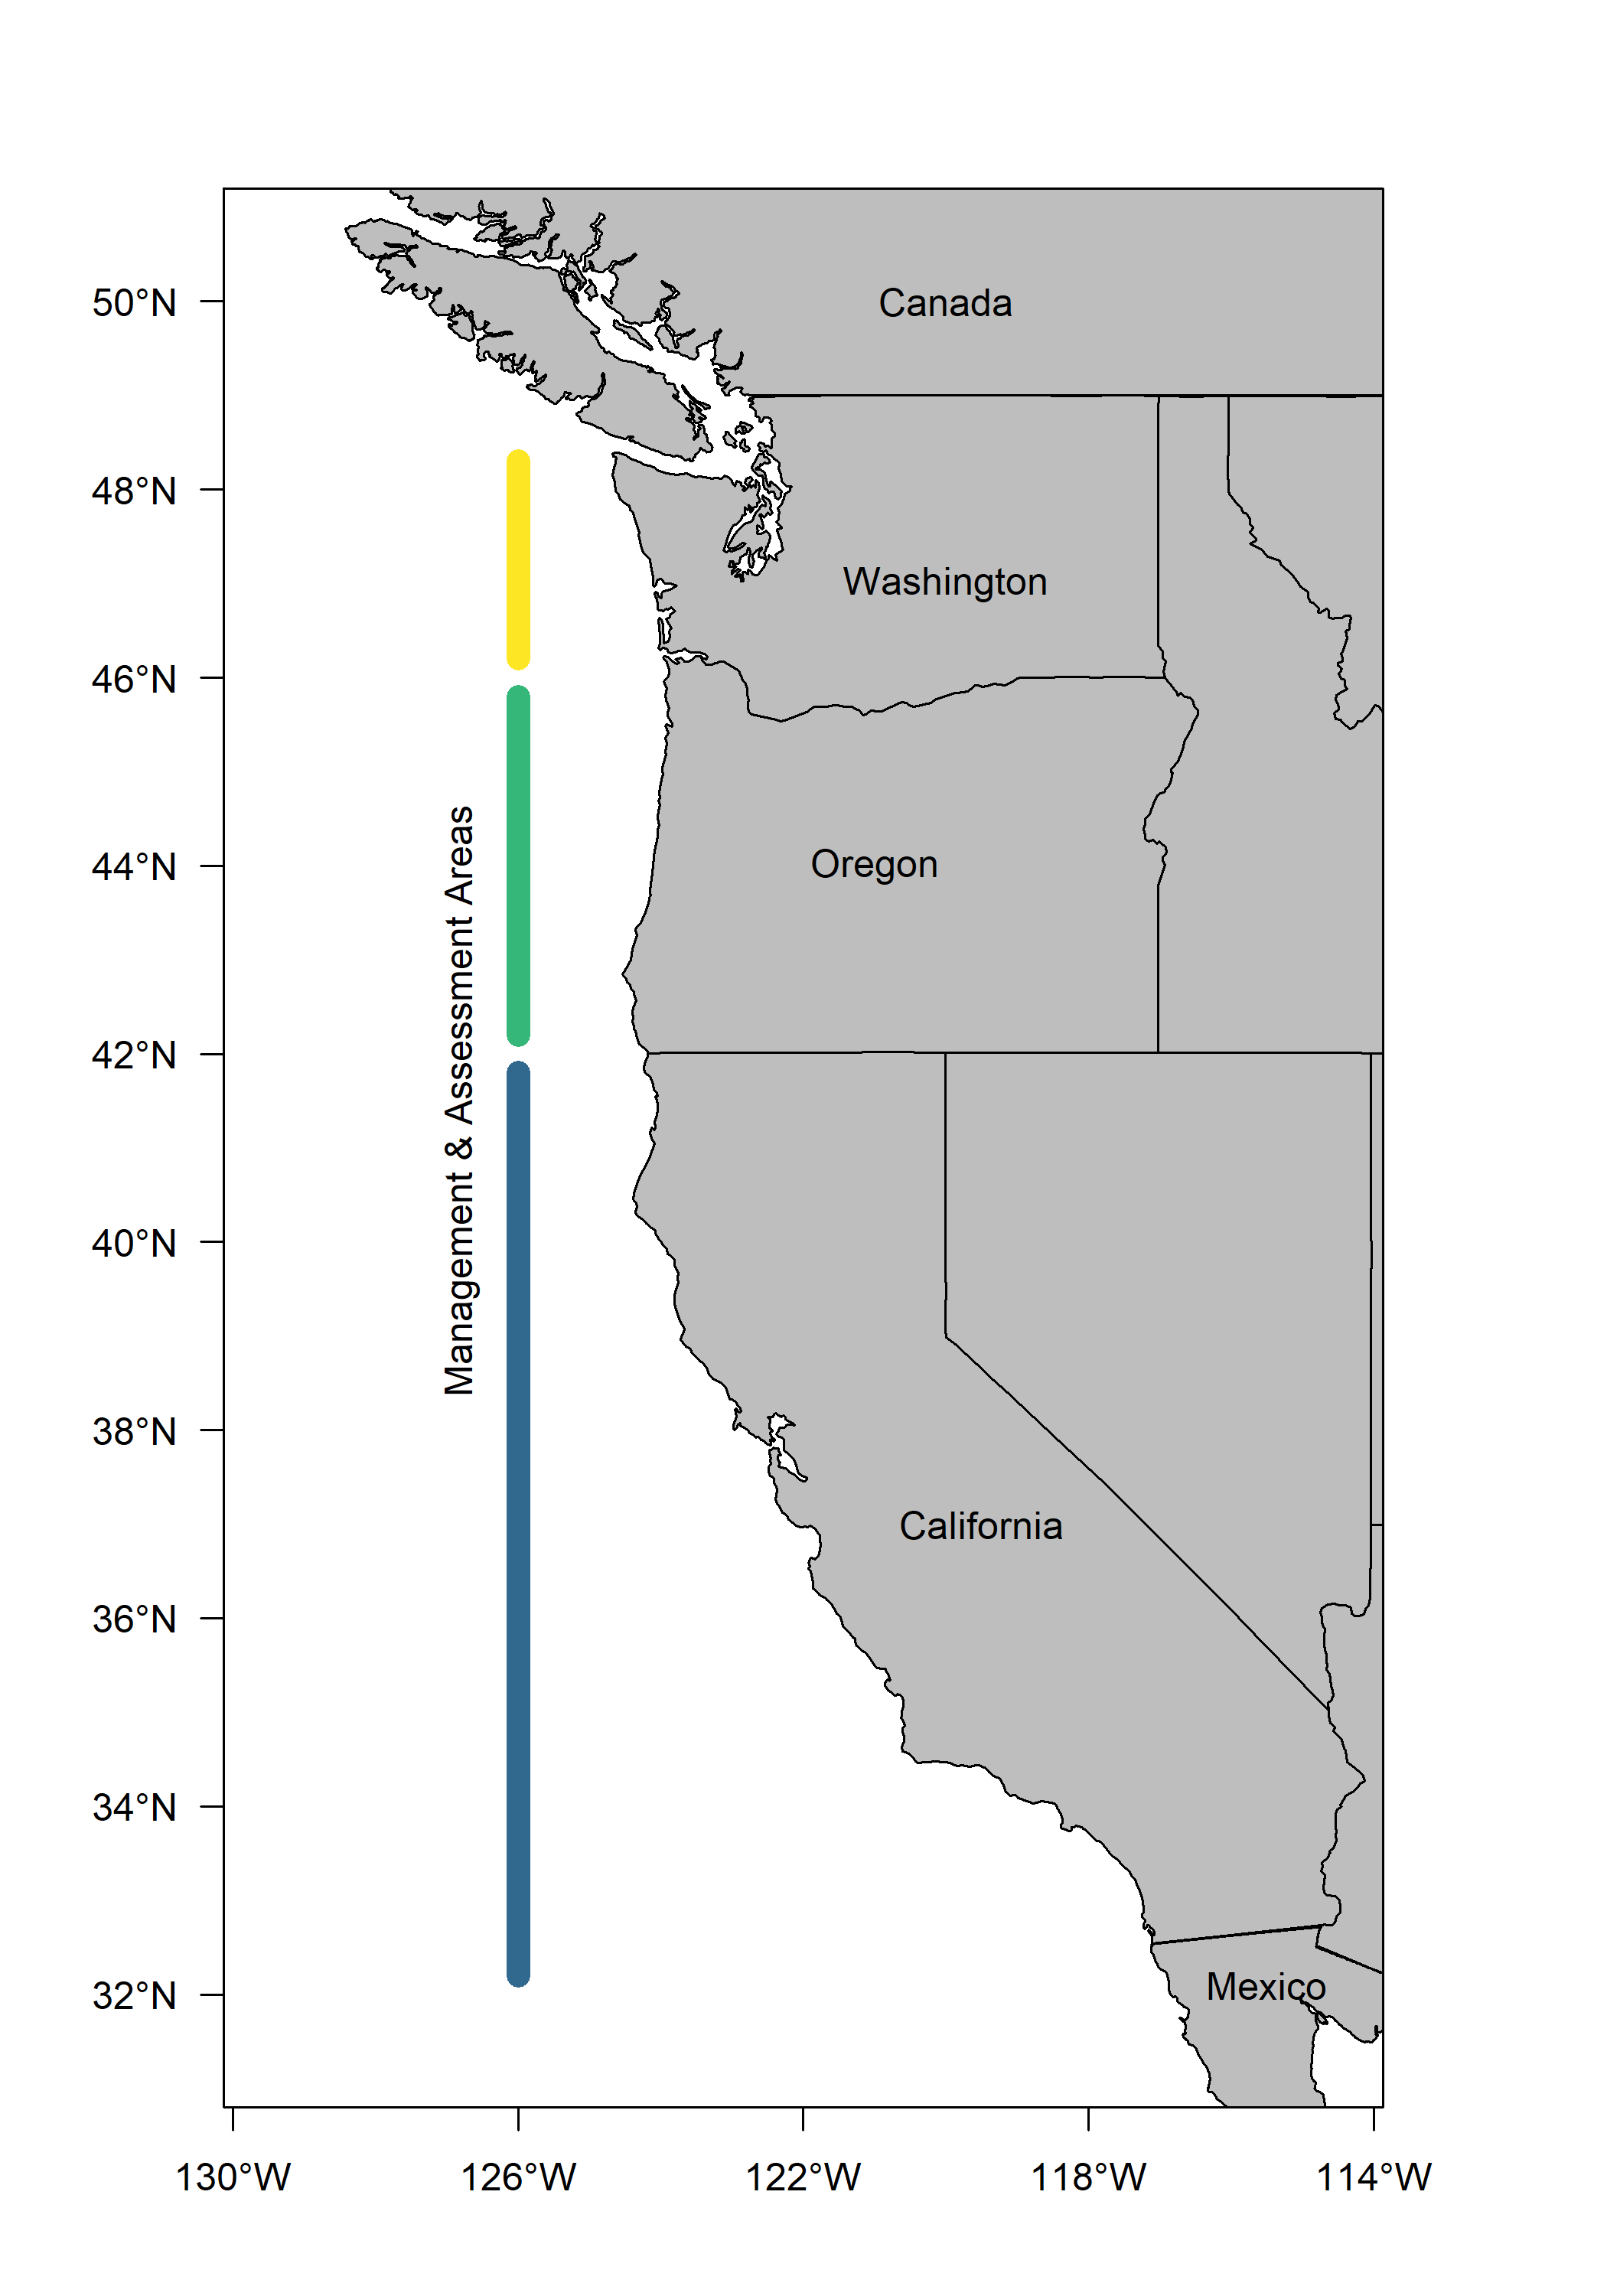
\includegraphics[width=1\textwidth,height=1\textheight]{C:/Users/Jason.Cope/Documents/Github/Sebastes_melanops_WA/Document/figures/stock/black_rockfish_map.png}
\caption{Map of the management and assessment areas for Black Rockfish.\label{fig:map}}
\end{figure}

\pagebreak

\begin{figure}
\centering
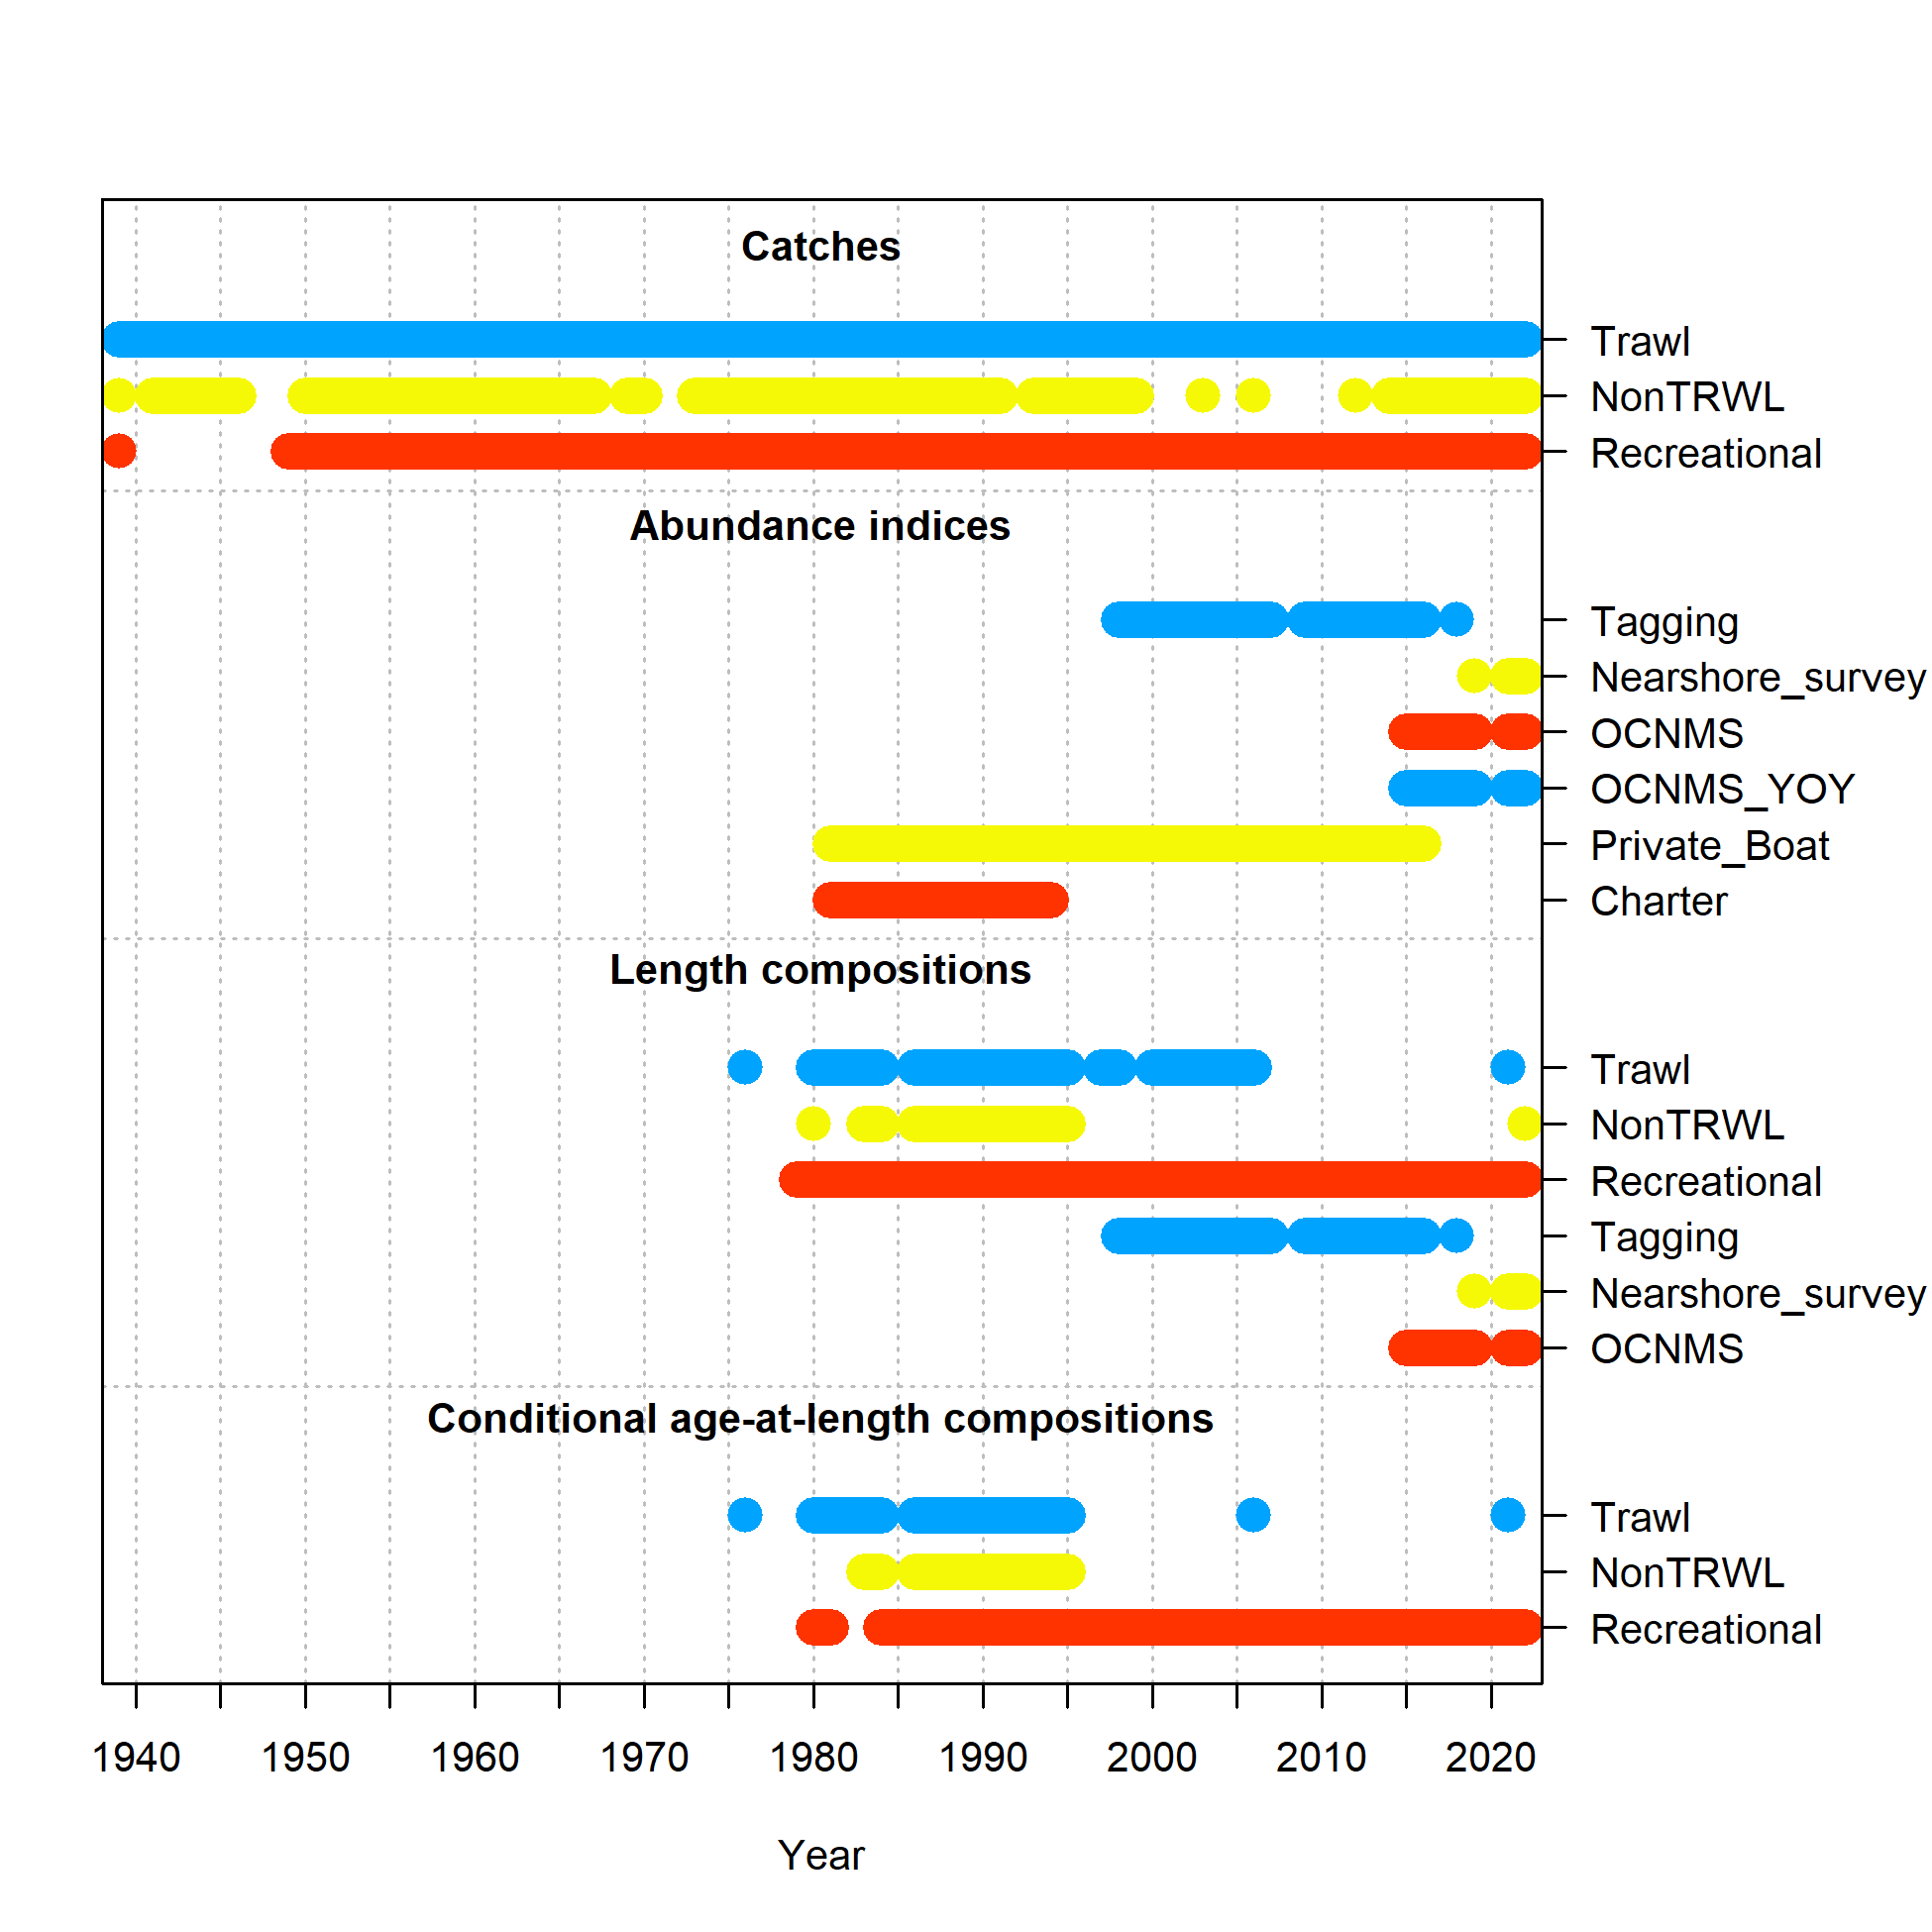
\includegraphics[width=1\textwidth,height=1\textheight]{C:/Users/Jason.Cope/Documents/Github/Sebastes_melanops_WA/Document/models/Reference model/plots/data_plot.png}
\caption{Summary of data sources used in the reference model.\label{fig:data-plot}}
\end{figure}

\pagebreak

\begin{figure}
\centering
\includegraphics[width=1\textwidth,height=1\textheight]{C:/Users/Jason.Cope/Documents/Github/Sebastes_melanops_WA/Document/models/Reference model/plots/catch-ts-comparison.png}
\caption{Comparison of total removals and removals by fleet between this assessment and those in 2007 and 2015. The lines showing the Non-Trawl and Recreational removal time series for the 2015 assessment cannot be seen as they are masked by the lines for the 2023 time series.\label{fig:catch-ts-comparison}}
\end{figure}

\pagebreak

\begin{figure}
\centering
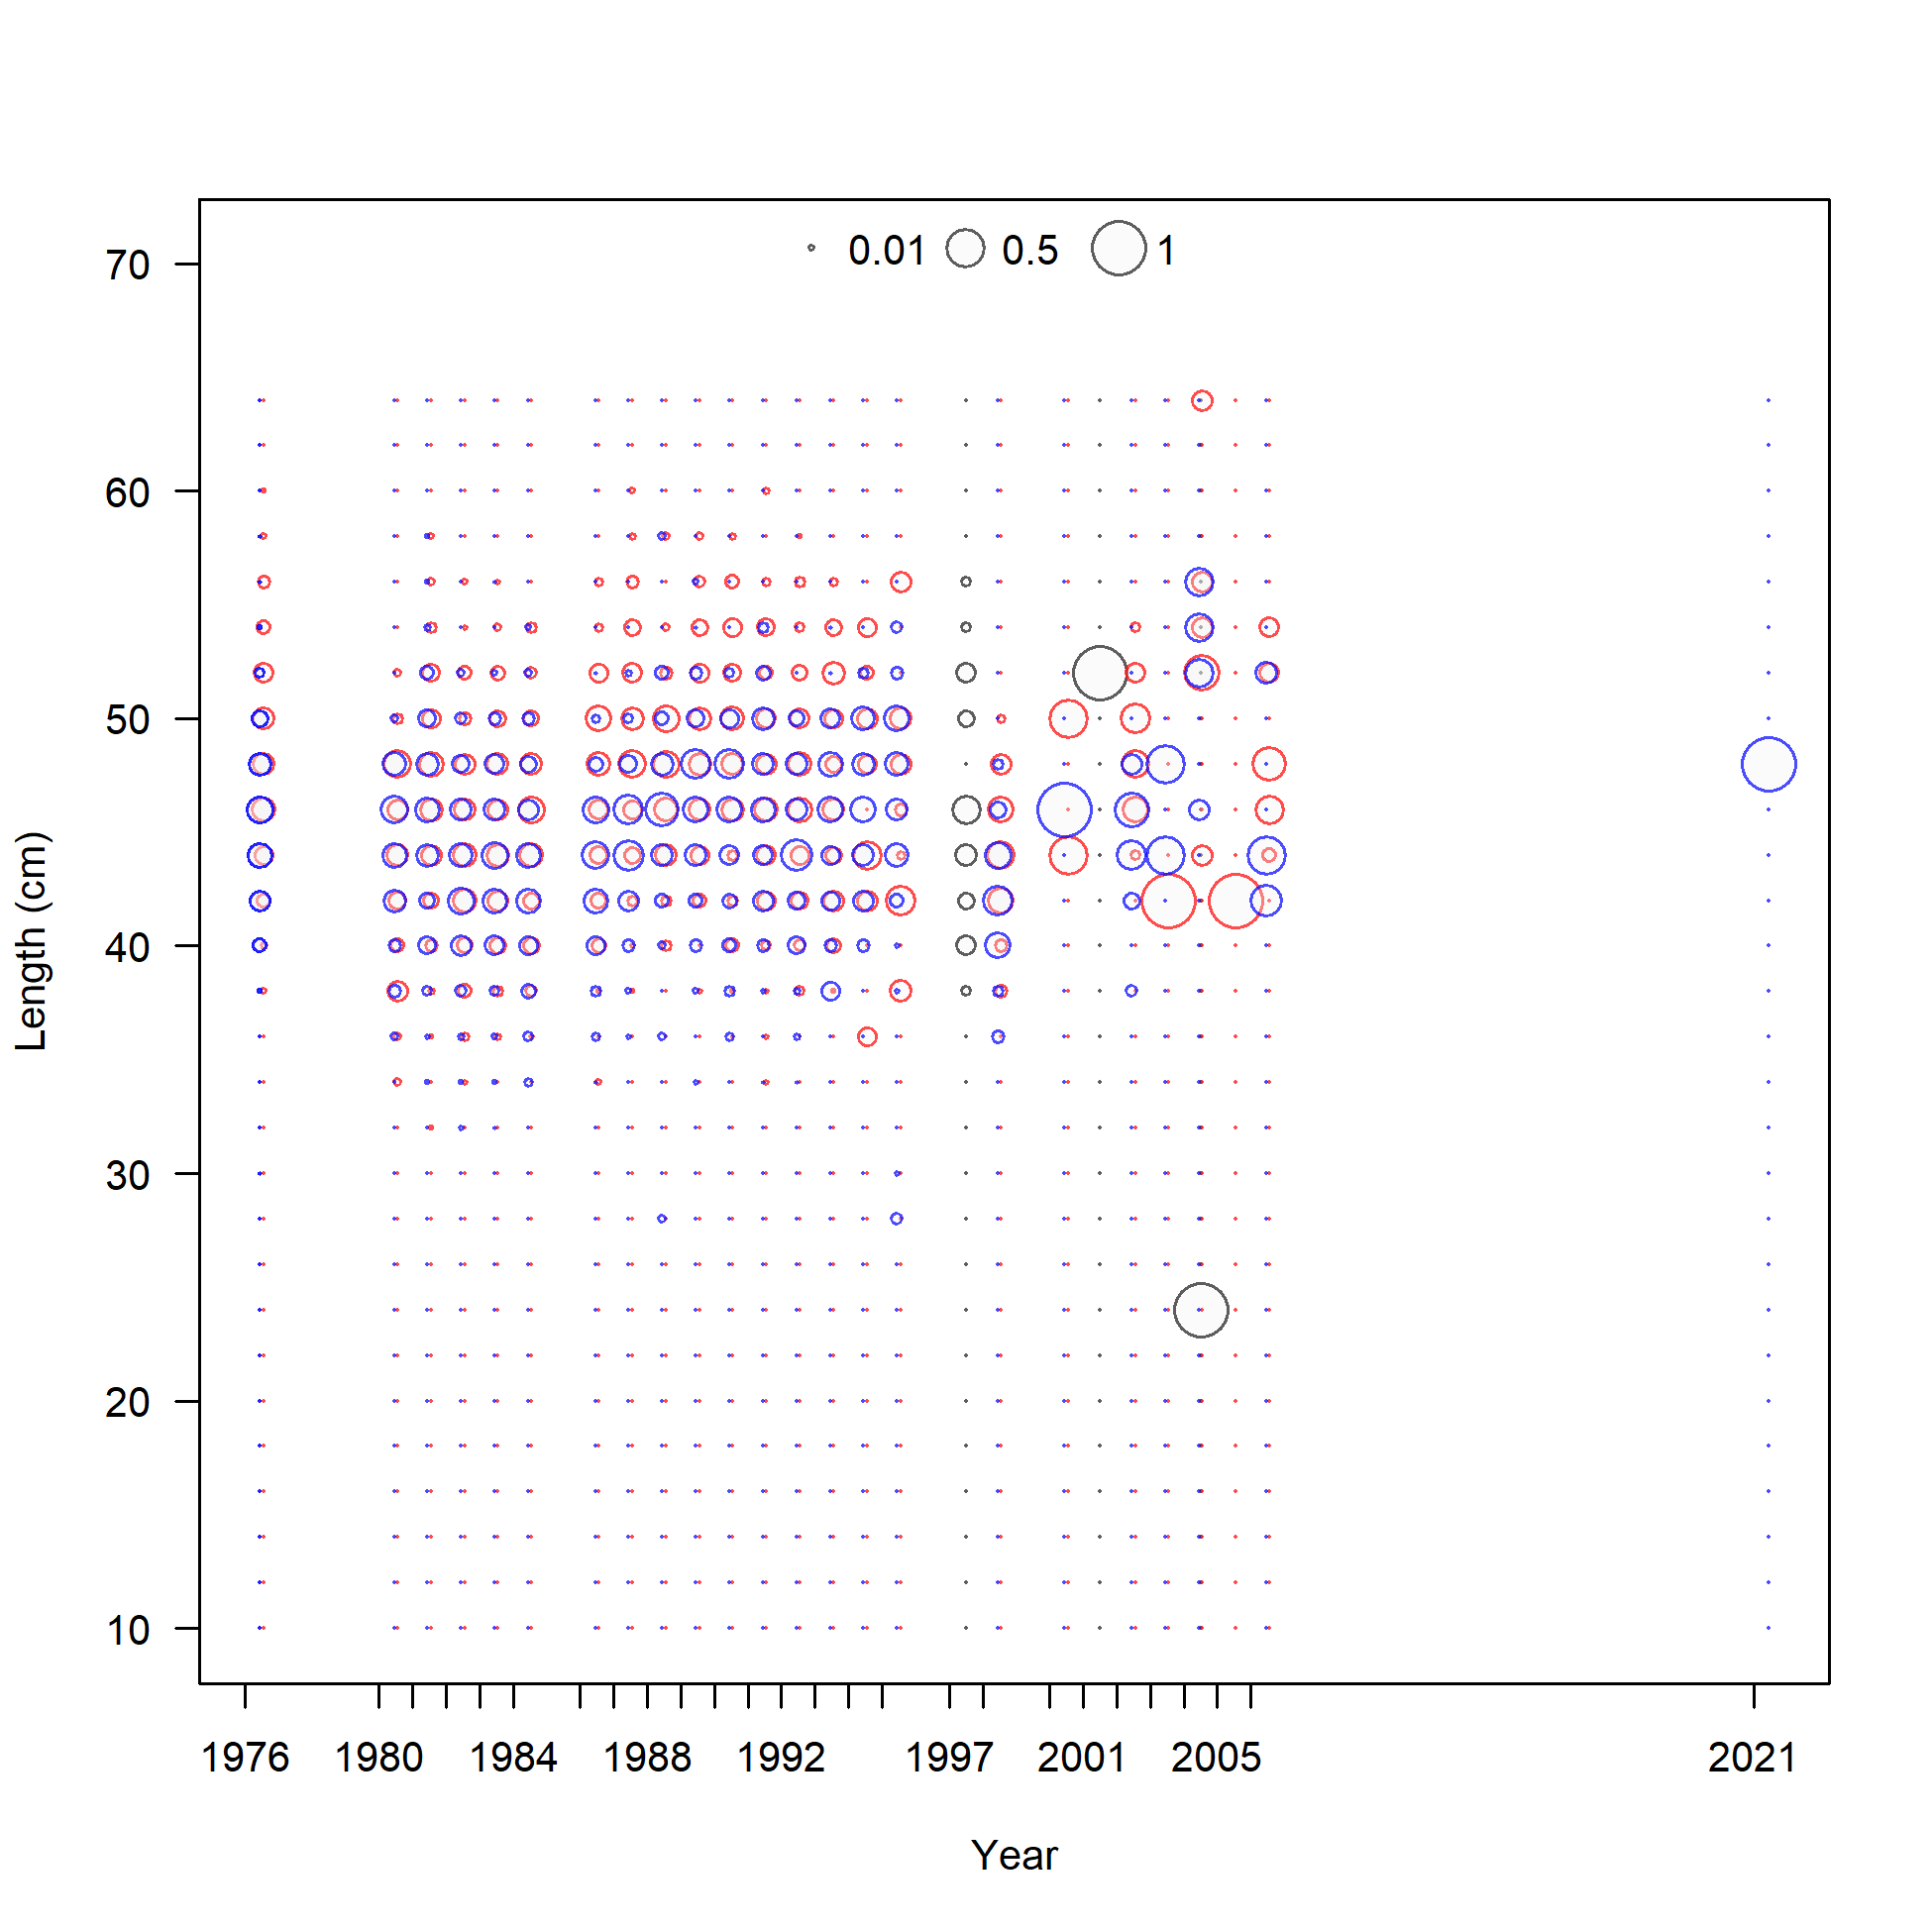
\includegraphics[width=1\textwidth,height=1\textheight]{C:/Users/Jason.Cope/Documents/Github/Sebastes_melanops_WA/Document/models/Reference model/plots/comp_lendat_bubflt1mkt0_page2.png}
\caption{Length compositions by year from the commercial trawl fleet.\label{fig:trawl-length-comps}}
\end{figure}

\pagebreak

\begin{figure}
\centering
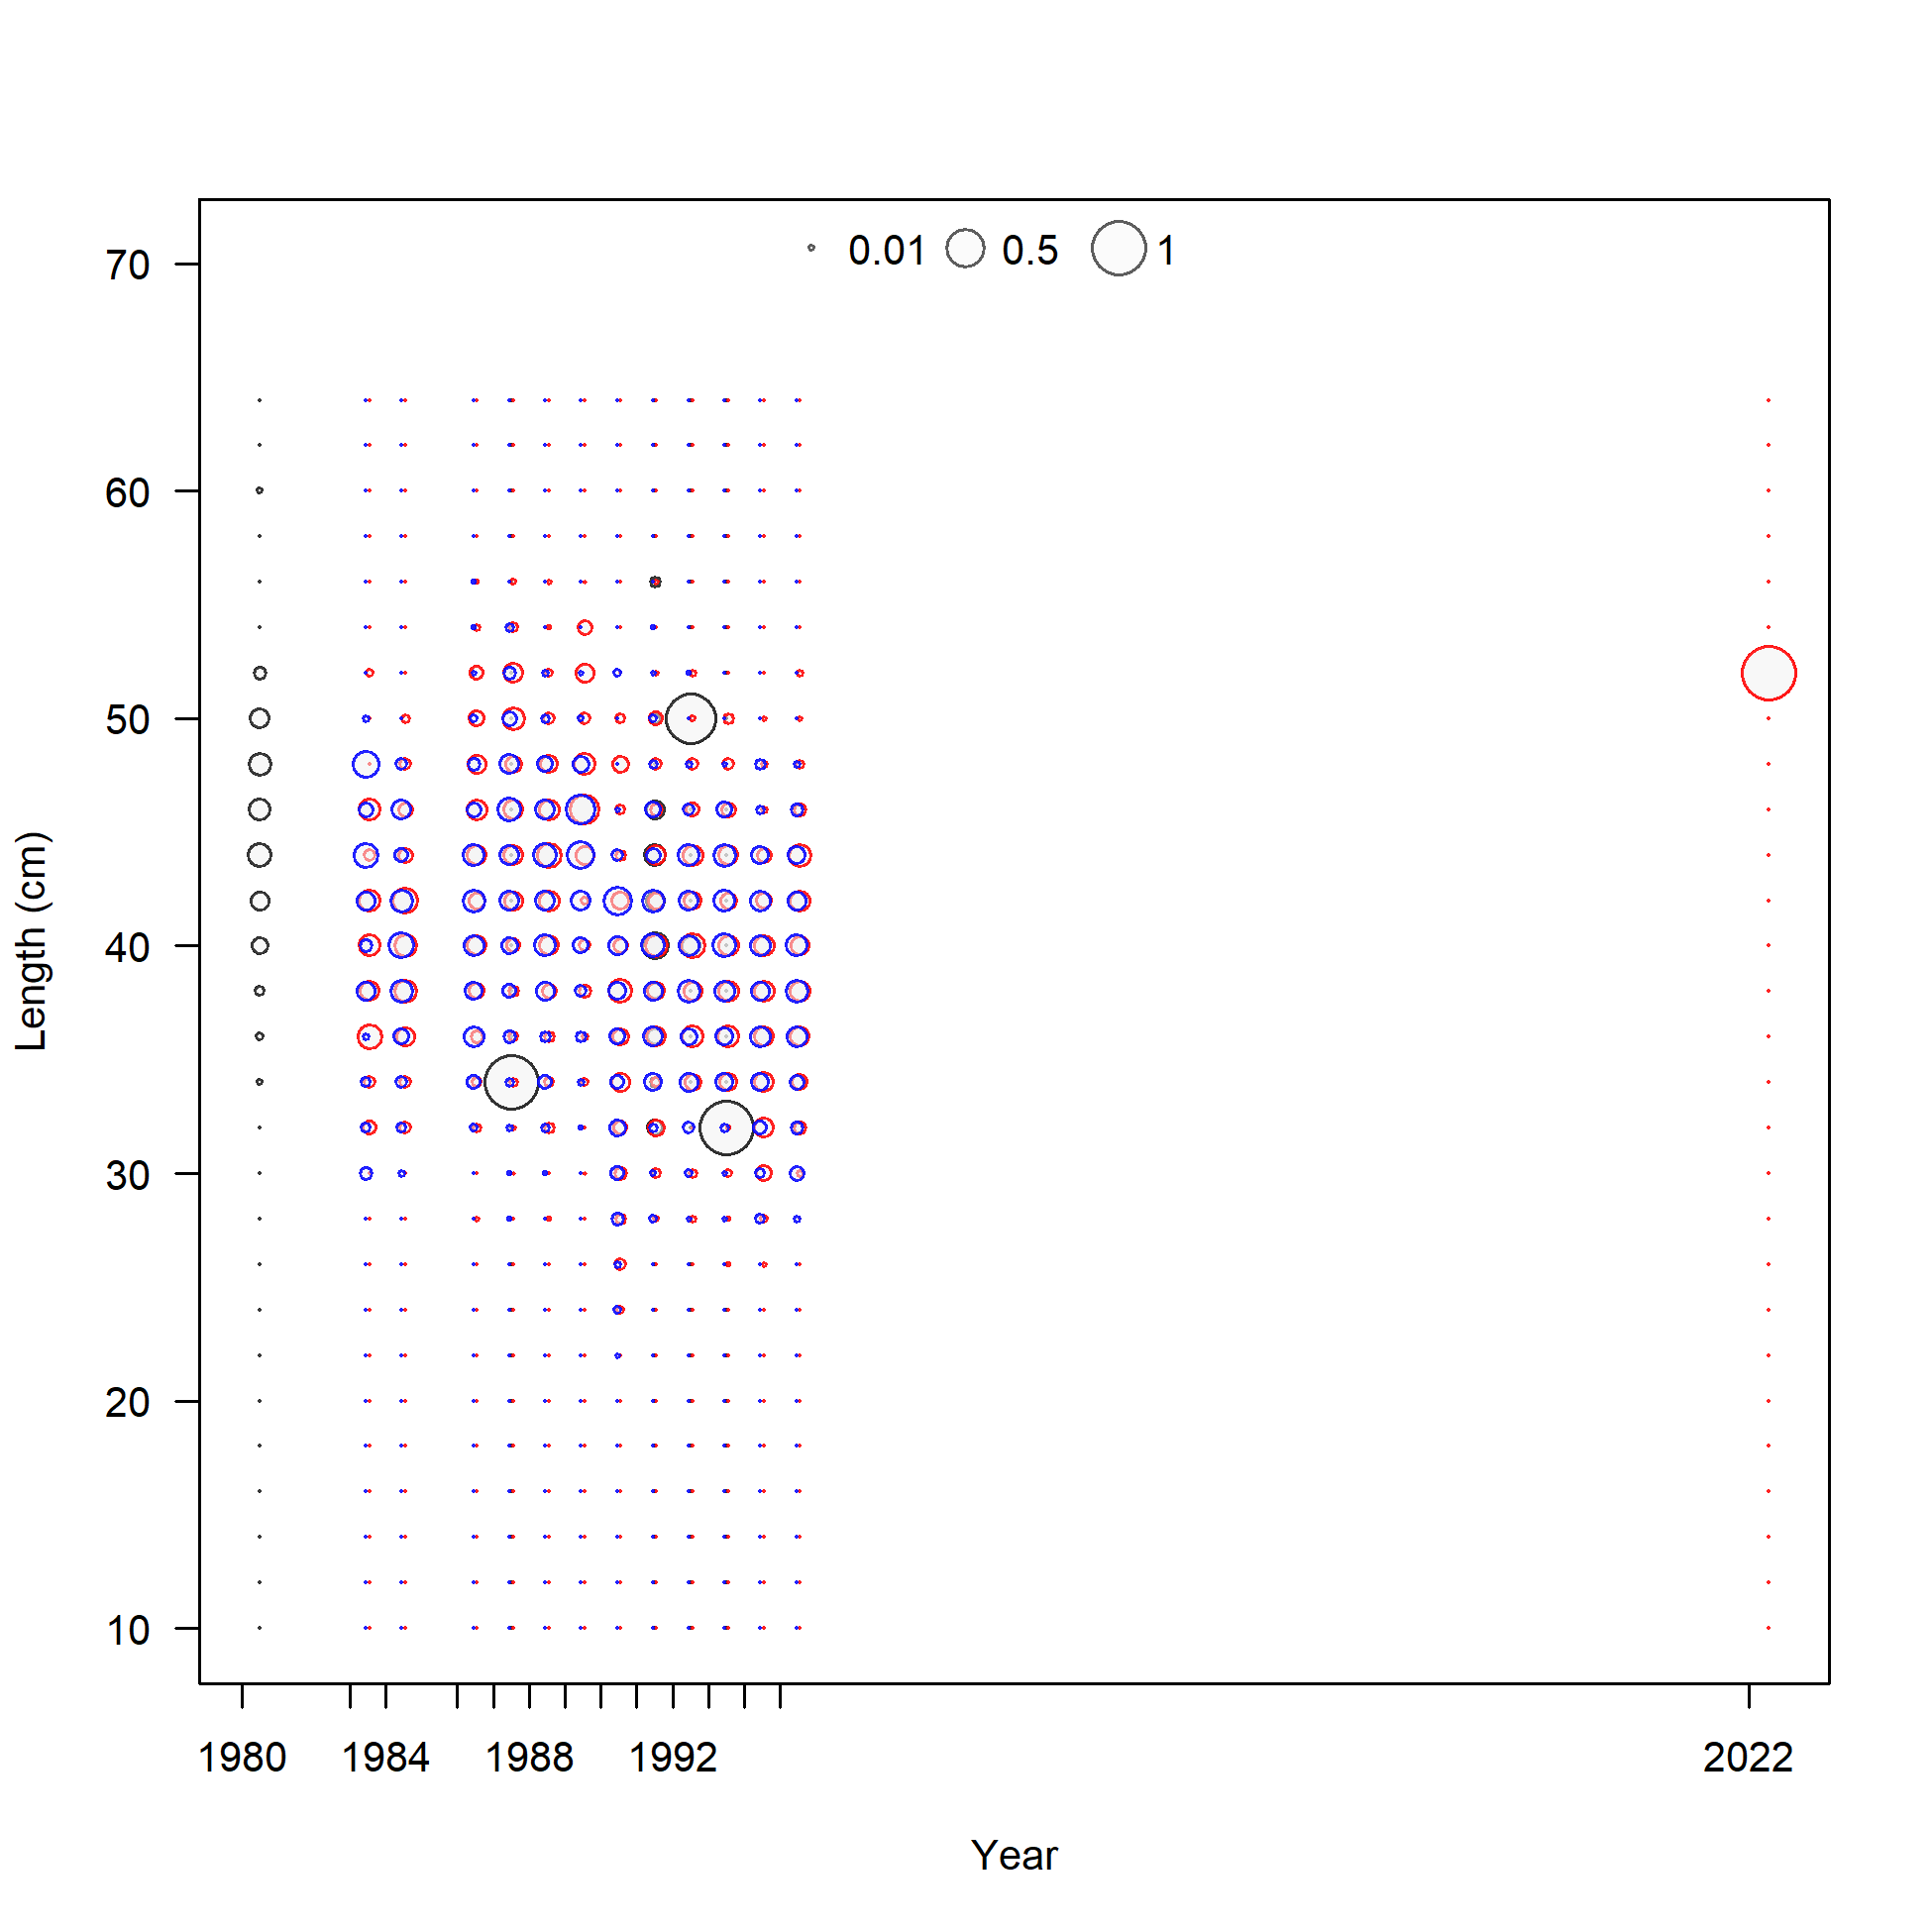
\includegraphics[width=1\textwidth,height=1\textheight]{C:/Users/Jason.Cope/Documents/Github/Sebastes_melanops_WA/Document/models/Reference model/plots/comp_lendat_bubflt2mkt0.png}
\caption{Length compositions by year from the commercial nontrawl fleet.\label{fig:nontrawl-length-comps}}
\end{figure}

\pagebreak

\begin{figure}
\centering
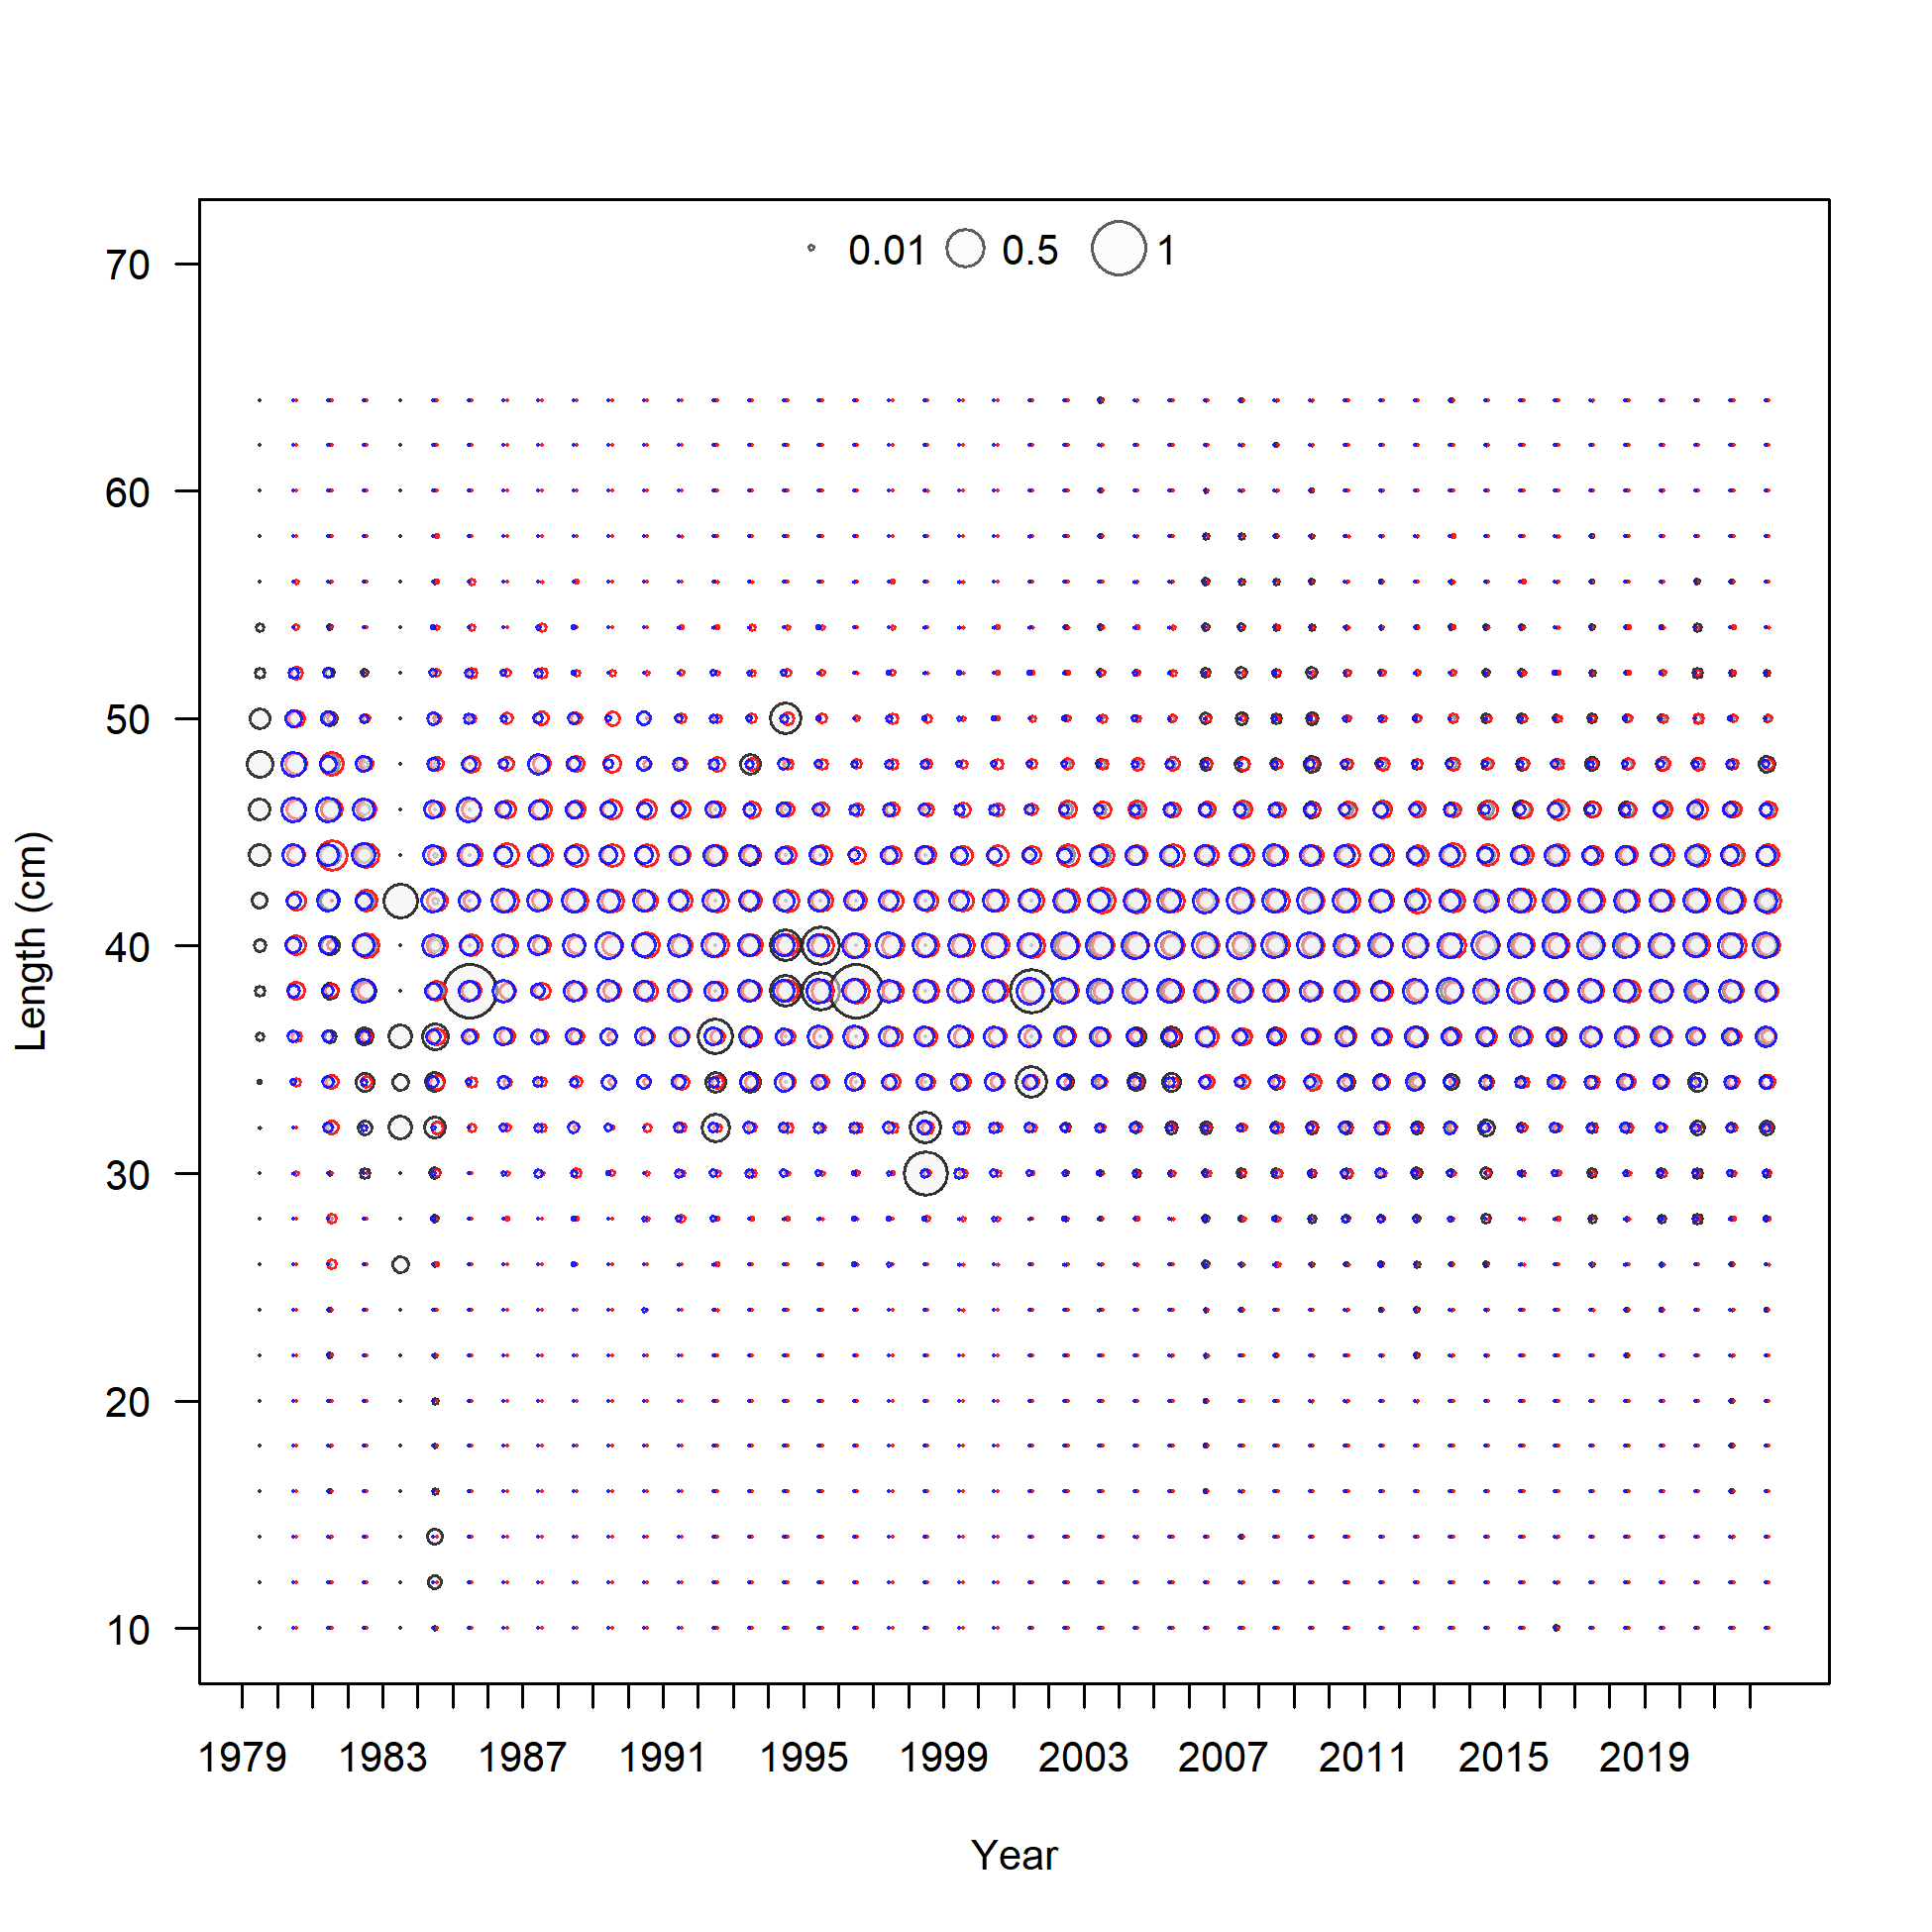
\includegraphics[width=1\textwidth,height=1\textheight]{C:/Users/Jason.Cope/Documents/Github/Sebastes_melanops_WA/Document/models/Reference model/plots/comp_lendat_bubflt3mkt0_page2.png}
\caption{Length compositions by year from the recreational fleet.\label{fig:rec-length-comps}}
\end{figure}

\pagebreak

\begin{figure}
\centering
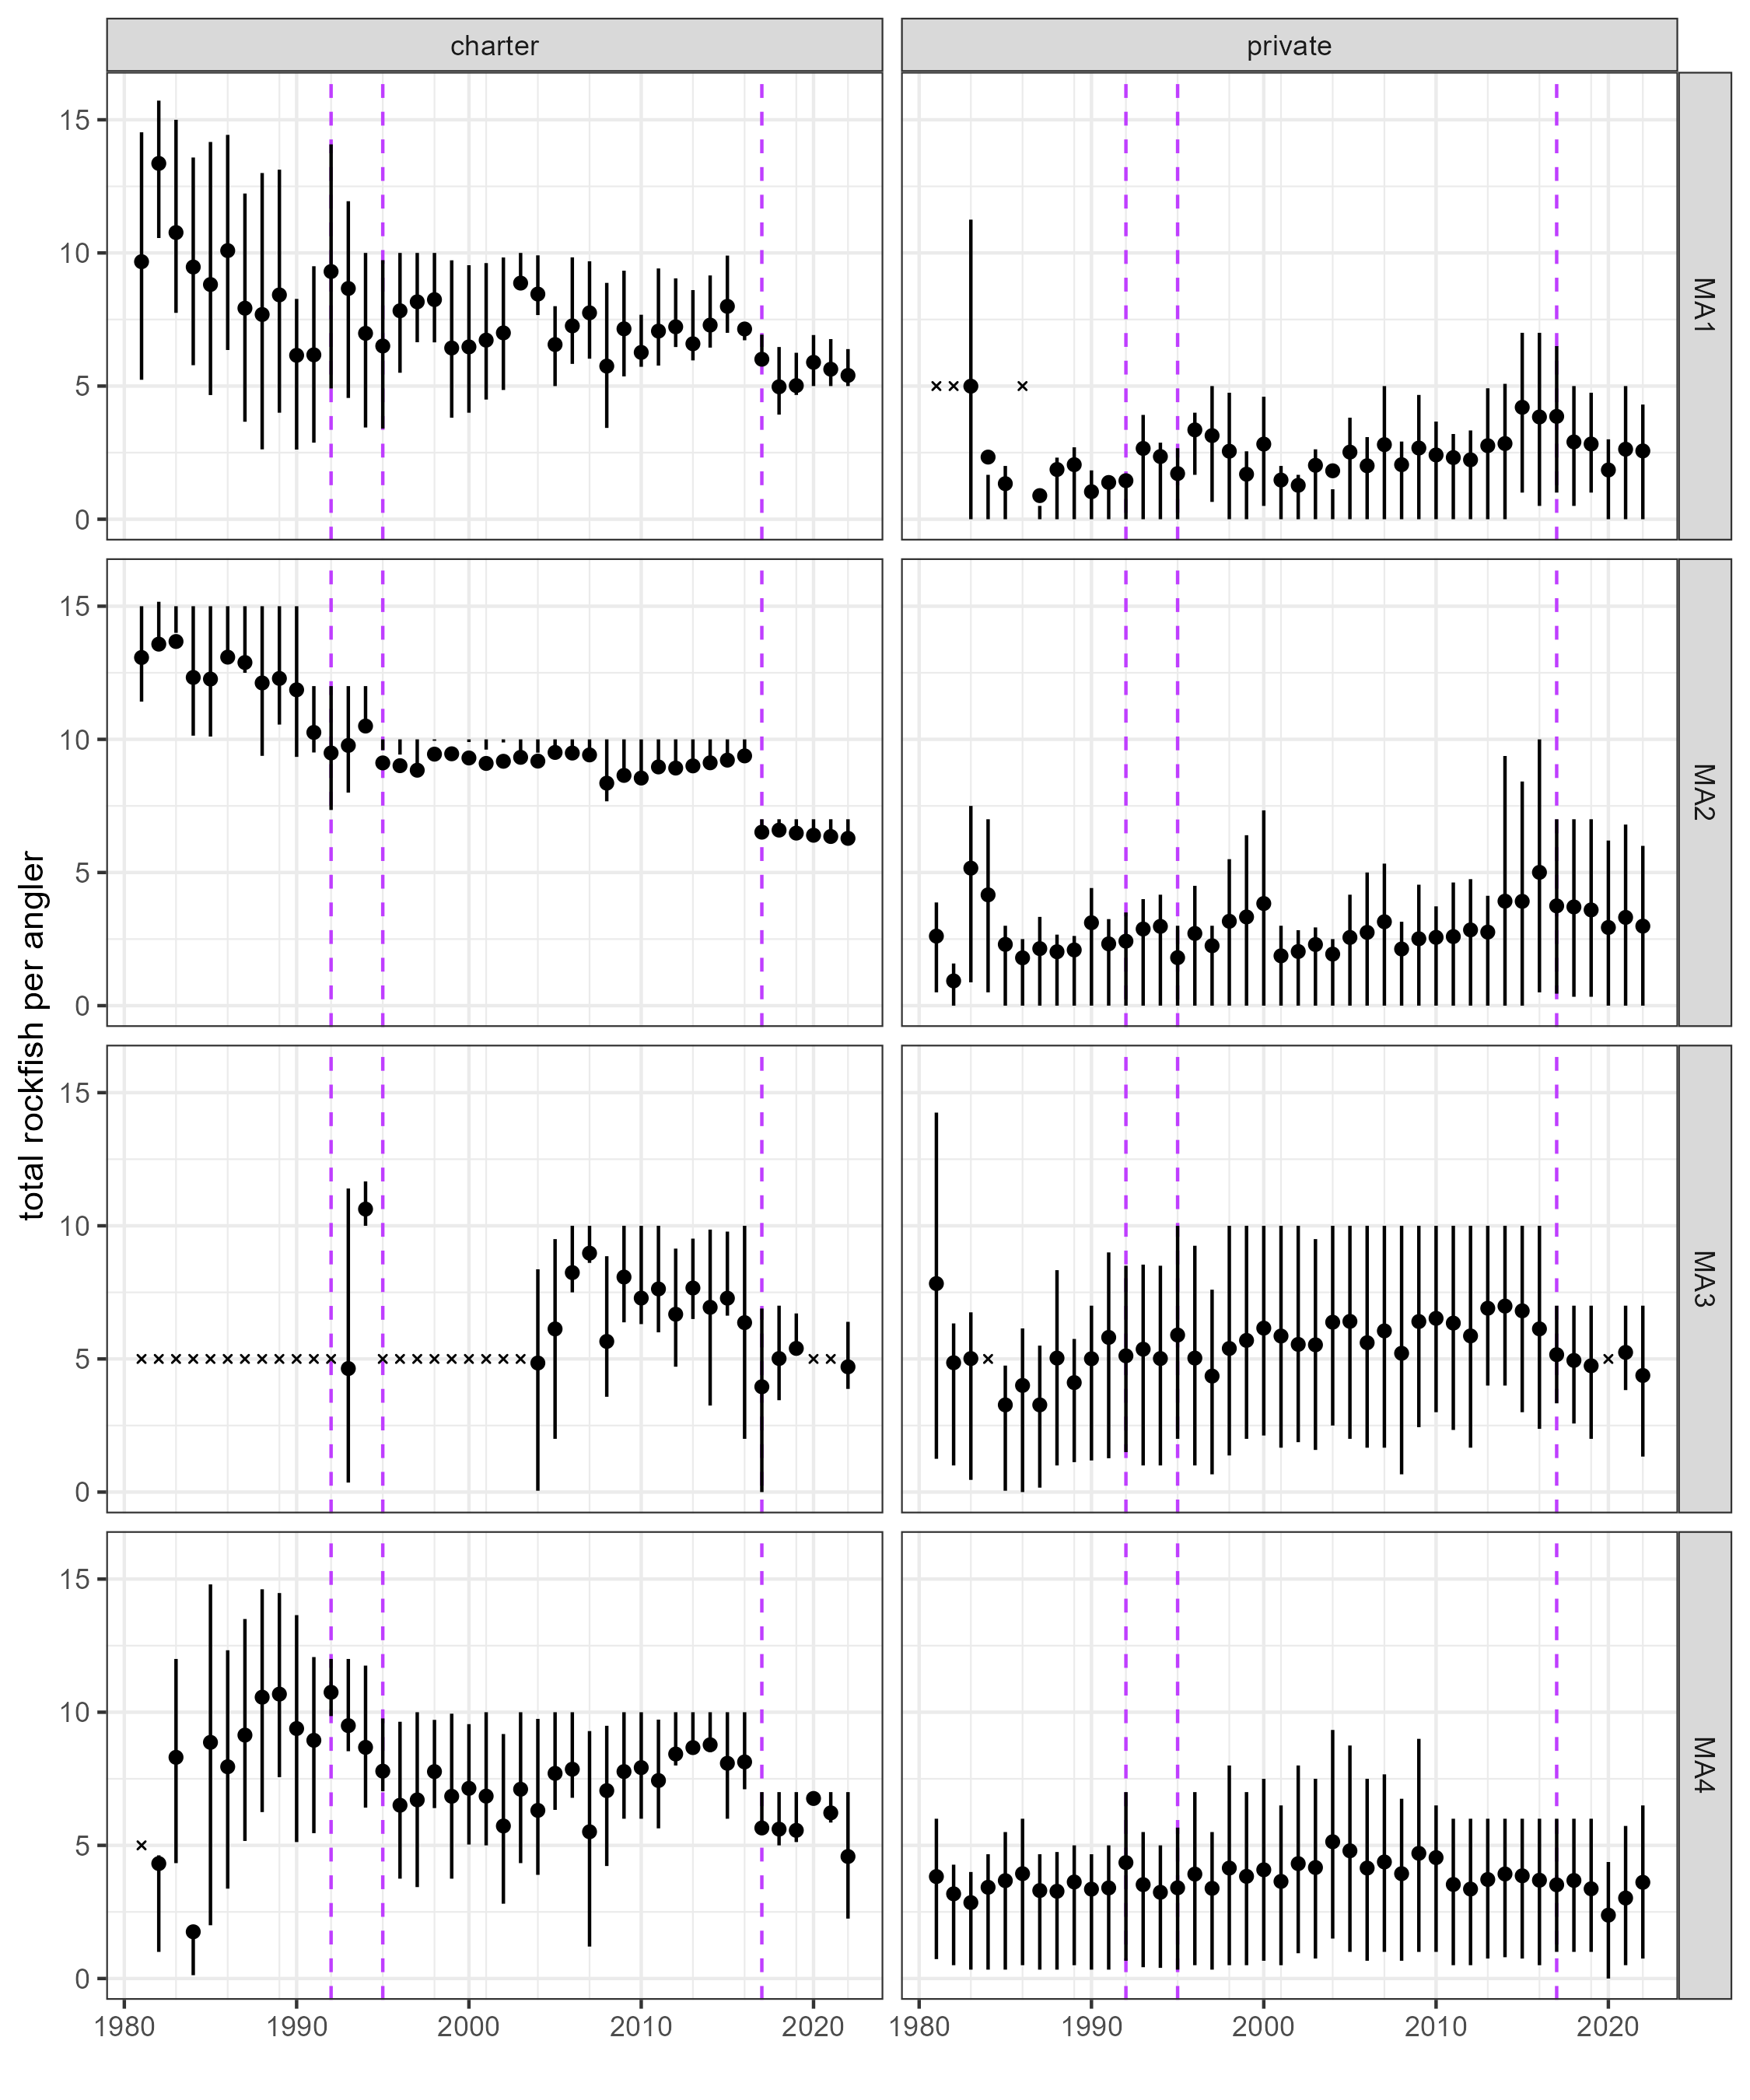
\includegraphics[width=1\textwidth,height=1\textheight]{C:/Users/Jason.Cope/Documents/Github/Sebastes_melanops_WA/Document/figures/index/OSP-rockfish-bag-limit-n-min10.png}
\caption{Trip average (points) and interquartile range (vertical solid lines) of the number of total rockfish retained per angler, 1981-2022, by boat type and marine area. Years in which there less than 10 records are indicated by the cross symbol. The vertical dashed lines indicate a change in the bag limit. Note that the bag limit change in 1992 did not apply to Marine Area 1.\label{fig:baglimit_numbers}}
\end{figure}

\pagebreak

\begin{figure}
\centering
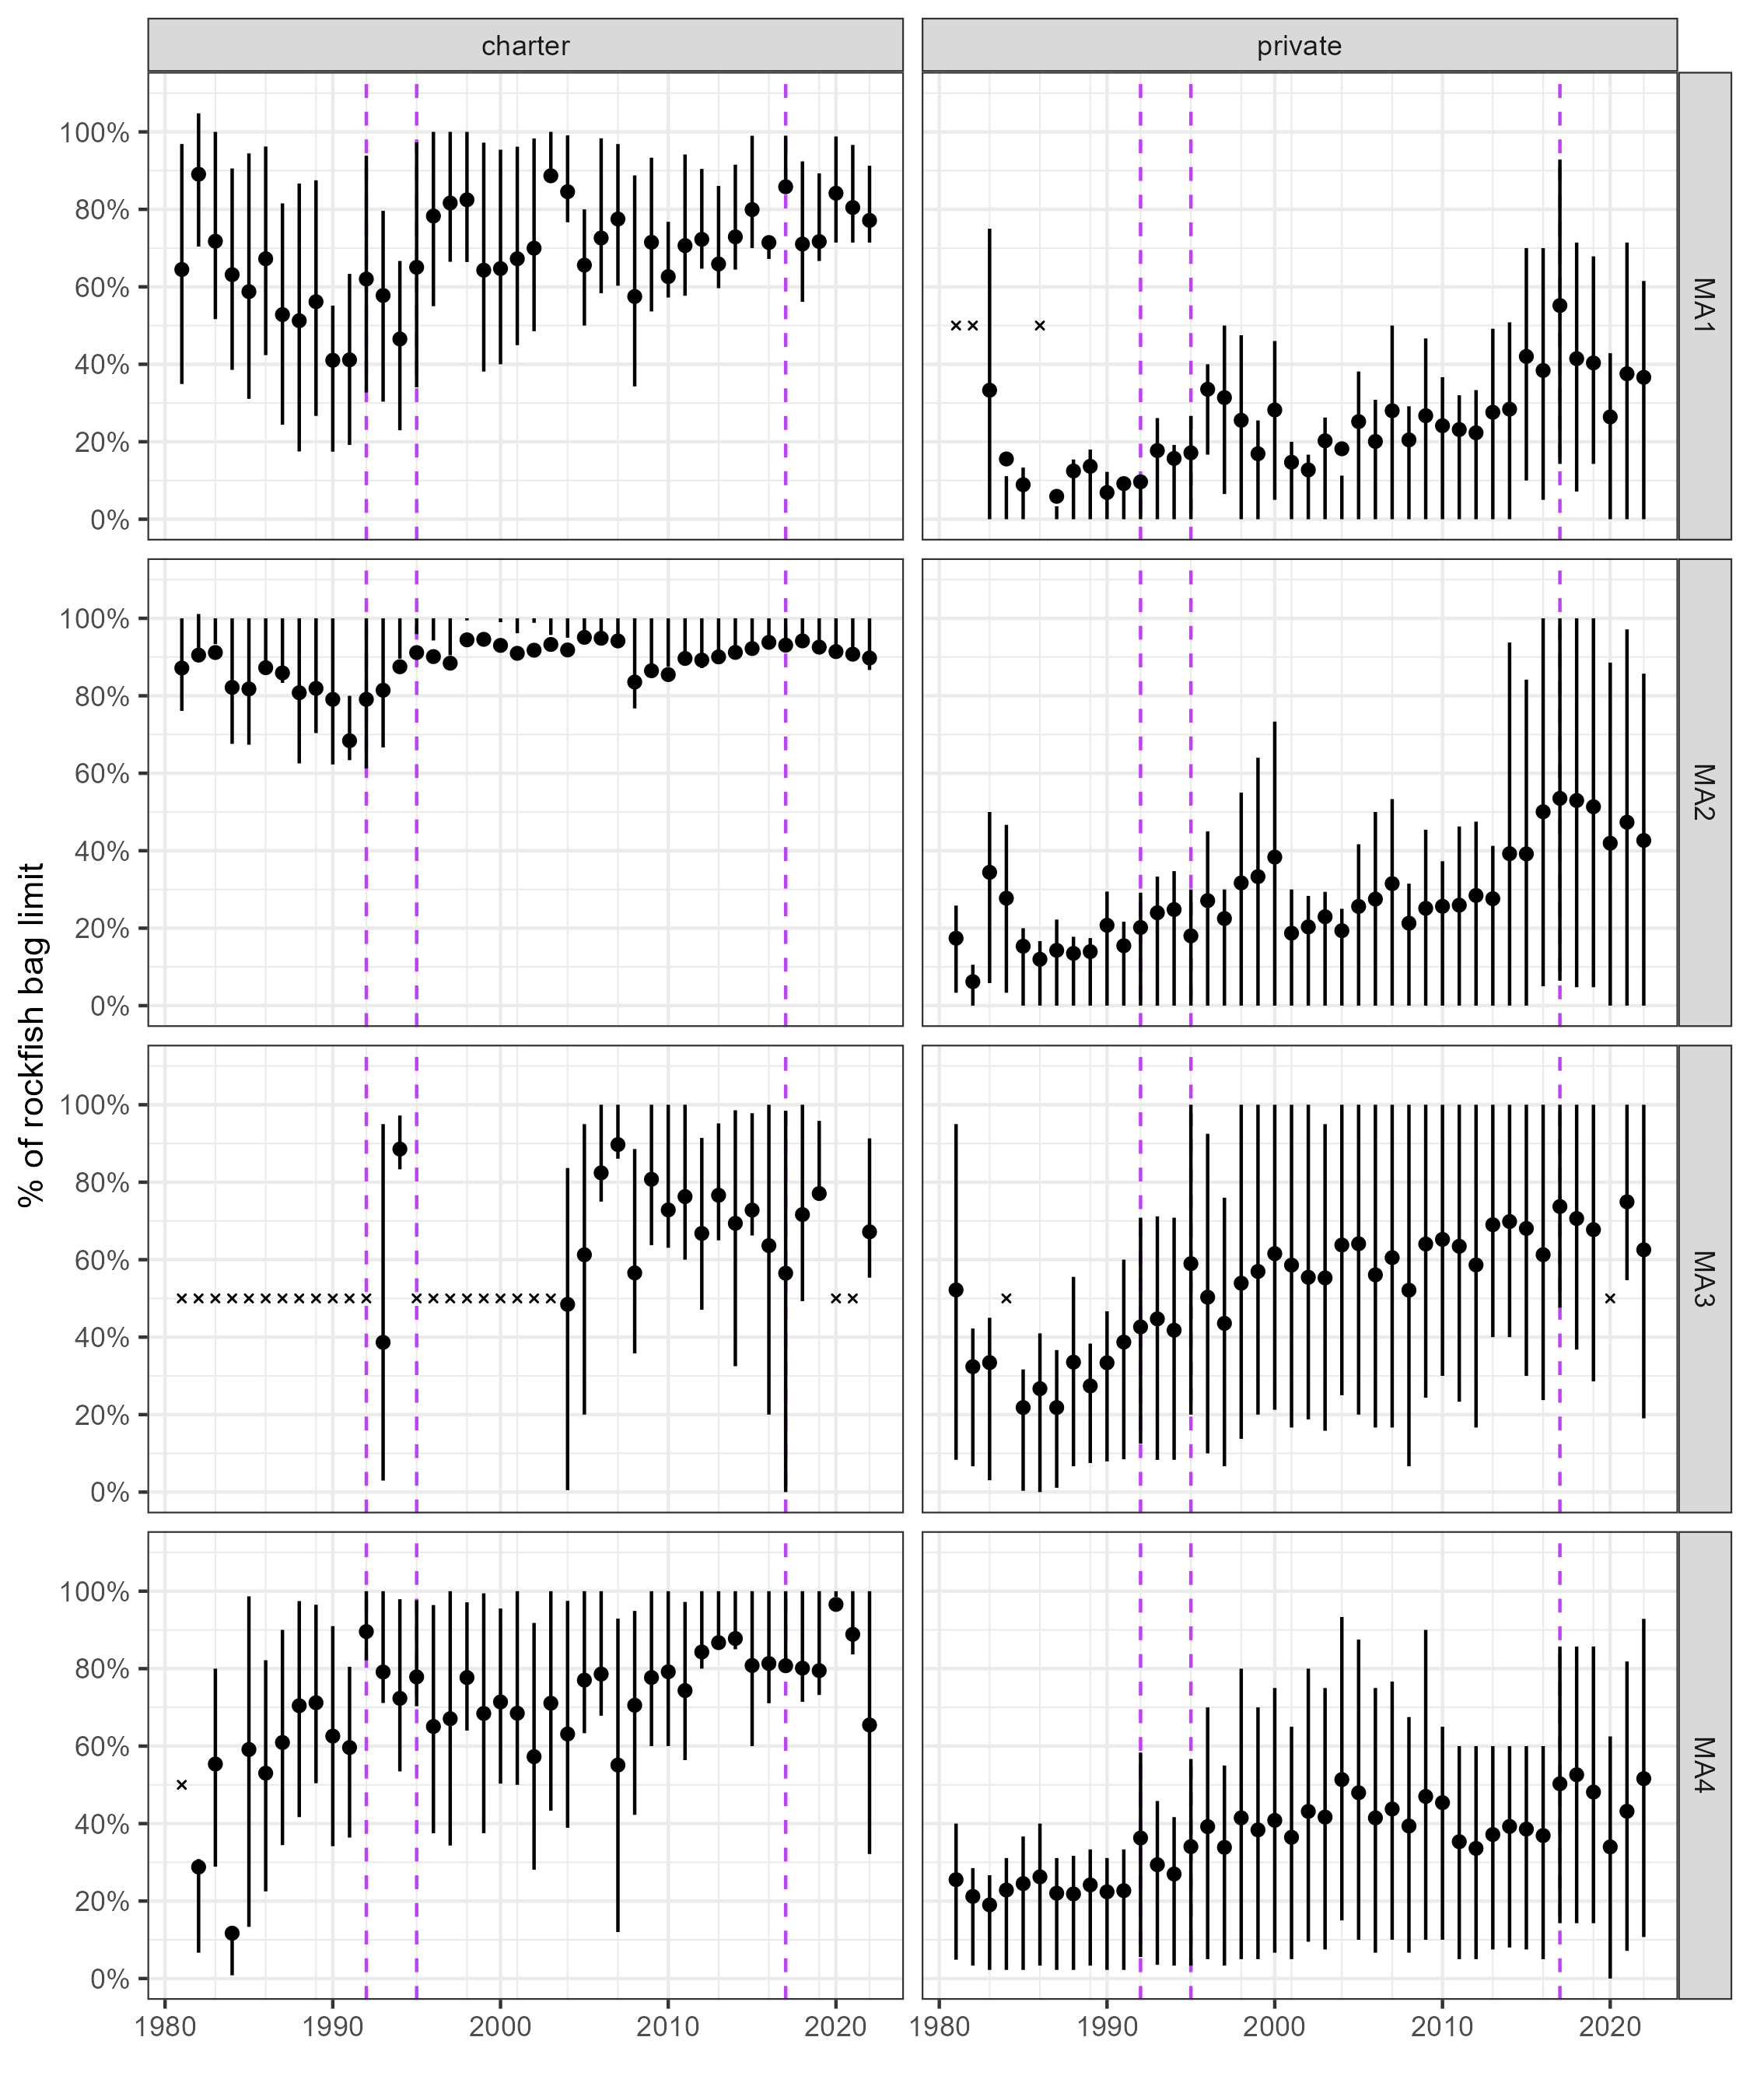
\includegraphics[width=1\textwidth,height=1\textheight]{C:/Users/Jason.Cope/Documents/Github/Sebastes_melanops_WA/Document/figures/index/OSP-rockfish-bag-limit-p-min10.png}
\caption{Trip average (points) and interquartile range (vertical solid lines) of the percentage of the rockfish bag limit reached, 1981-2022, by boat type and marine area. Years in which there less than 10 records are indicated by the cross symbol. The vertical dashed lines indicate a change in the bag limit. Note that the bag limit change in 1992 did not apply to Marine Area 1.\label{fig:baglimit_percentage}}
\end{figure}

\pagebreak

\begin{figure}
\centering
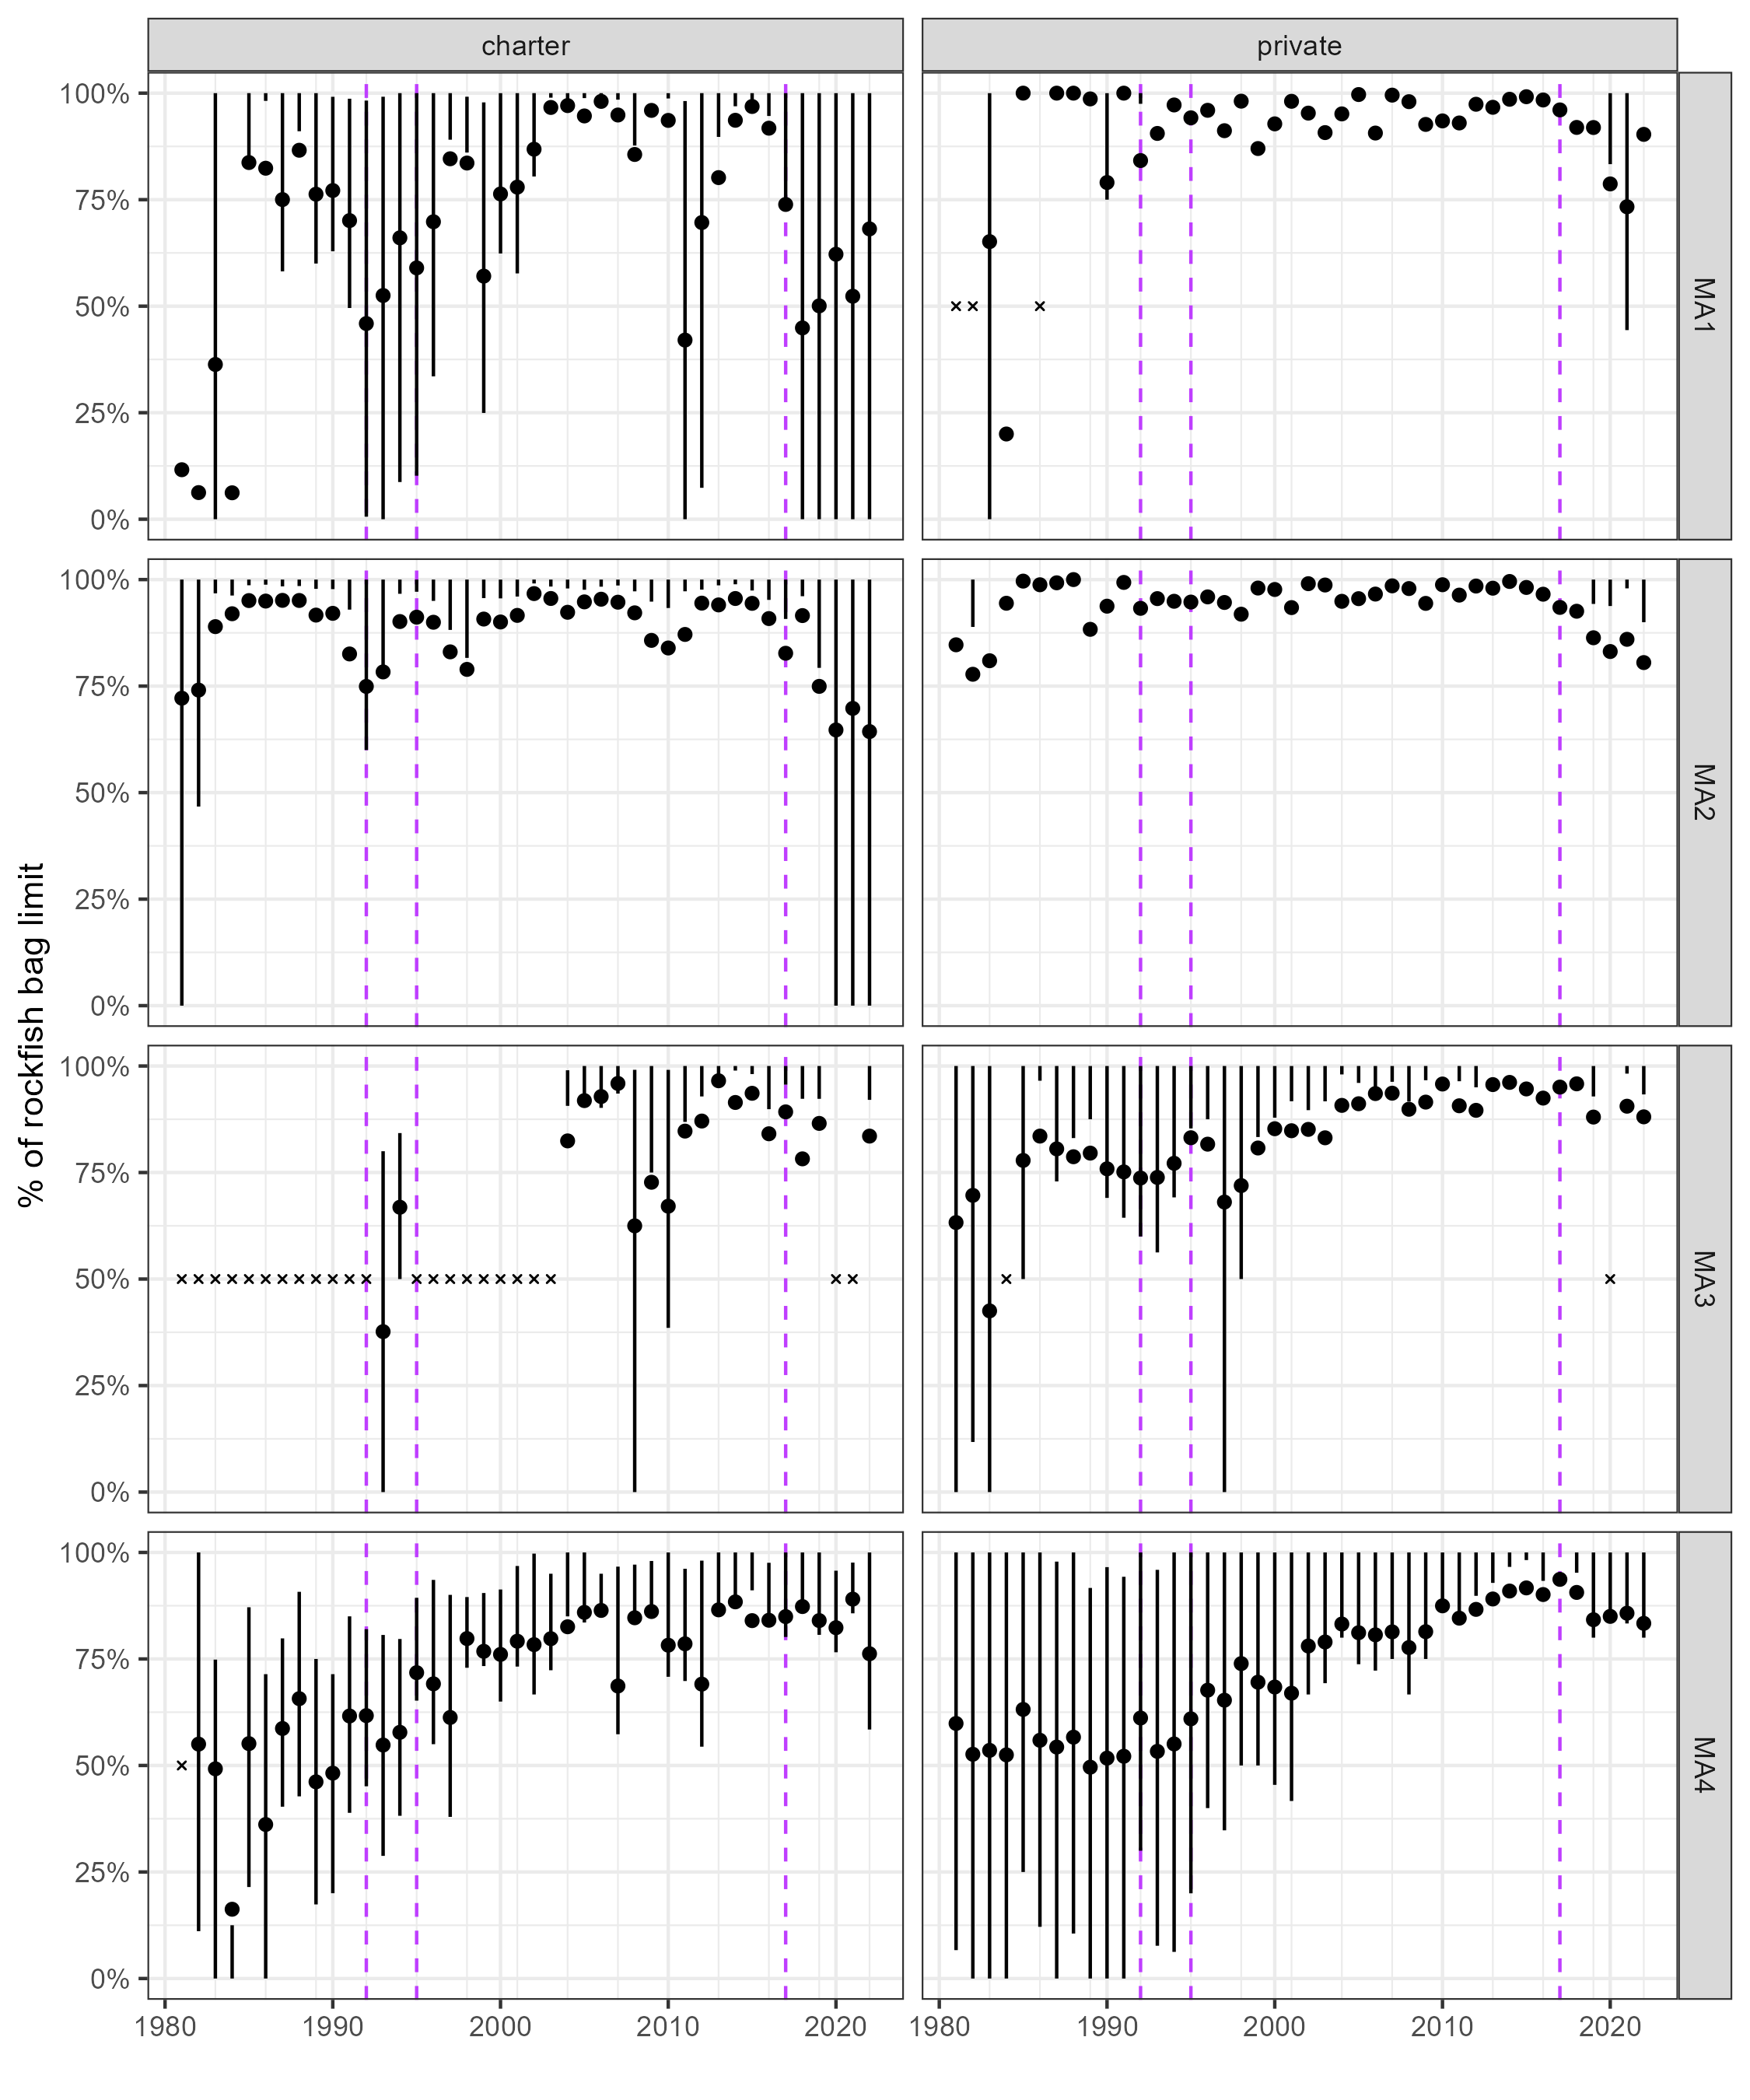
\includegraphics[width=1\textwidth,height=1\textheight]{C:/Users/Jason.Cope/Documents/Github/Sebastes_melanops_WA/Document/figures/index/OSP_blackrock_p_total_rockfish.png}
\caption{Trip average (points) and interquartile range (vertical solid lines) of the percentage of total rockfish retained that were Black Rockfish, 1981-2022, by boat type and marine area. Years in which there less than 10 records are indicated by the cross symbol. The vertical dashed lines indicate a change in the bag limit. Note that the bag limit change in 1992 did not apply to Marine Area 1.\label{fig:blackrock_percentage}}
\end{figure}

\pagebreak

\begin{figure}
\centering
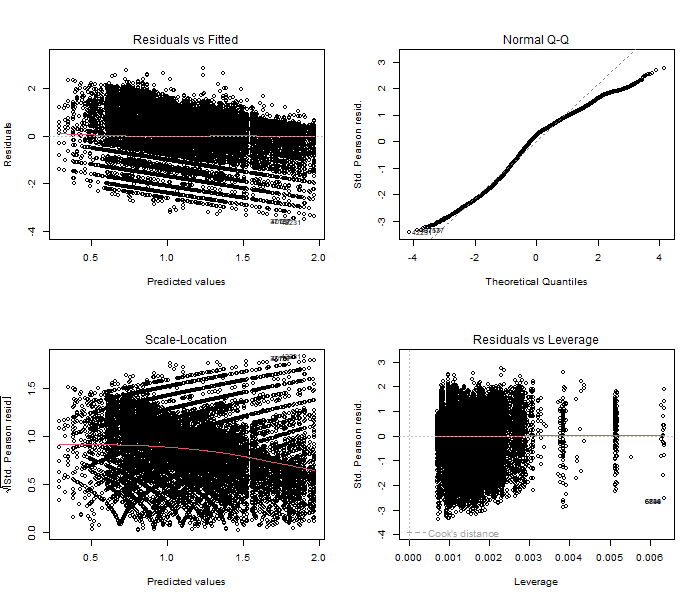
\includegraphics[width=1\textwidth,height=1\textheight]{C:/Users/Jason.Cope/Documents/Github/Sebastes_melanops_WA/Document/figures/index/GLMdiagnostics lognormal_Private.png}
\caption{Diagnostic plots for the positive catch component of the lognormal delta-GLM model for the Washington private boat Black Rockfish dataset. These plots are used to evaluate model fit (top left), assumptions of normality (top right), assumptions of constant variance (bottom left), and the presence of outliers (bottom right).\label{fig:private-log-diags}}
\end{figure}

\pagebreak

\begin{figure}
\centering
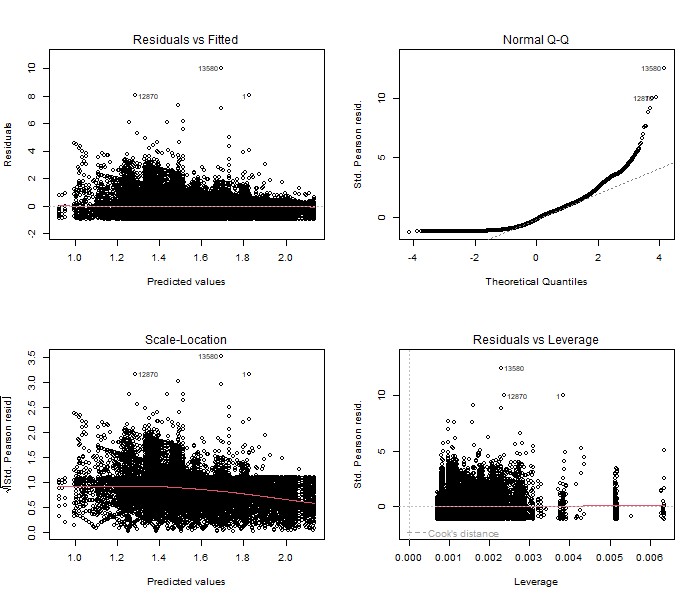
\includegraphics[width=1\textwidth,height=1\textheight]{C:/Users/Jason.Cope/Documents/Github/Sebastes_melanops_WA/Document/figures/index/GLMdiagnostics gamma_Private.png}
\caption{Diagnostic plots for the positive catch component of the gamma delta-GLM model for the Washington private boat Black Rockfish dataset. These plots are used to evaluate model fit (top left), assumptions of normality (top right), assumptions of constant variance (bottom left), and the presence of outliers (bottom right).\label{fig:private-gam-diags}}
\end{figure}

\pagebreak

\begin{figure}
\centering
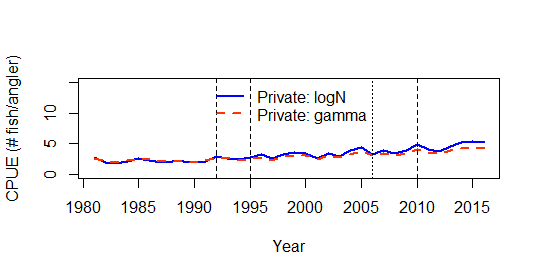
\includegraphics[width=1\textwidth,height=1\textheight]{C:/Users/Jason.Cope/Documents/Github/Sebastes_melanops_WA/Document/figures/index/WA_dockside_Private_Index.png}
\caption{Abundance indices for the WDFW private boat CPUE analysis. Vertical lines are notable management actions (mainly bag limit changes). Colors and line type indicates different distributional treatments of the index.\label{fig:private-index}}
\end{figure}

\pagebreak

\begin{figure}
\centering
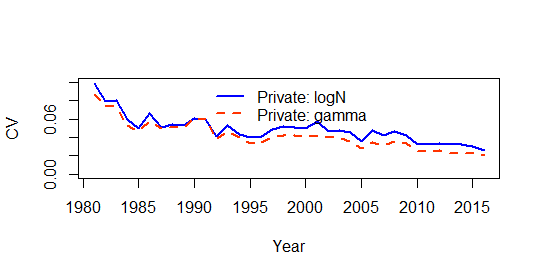
\includegraphics[width=1\textwidth,height=1\textheight]{C:/Users/Jason.Cope/Documents/Github/Sebastes_melanops_WA/Document/figures/index/WA_dockside_private_CV.png}
\caption{Bootstrapped estimates of variation for each model of the Washington private boat index.\label{fig:private-CVs}}
\end{figure}

\pagebreak

\begin{figure}
\centering
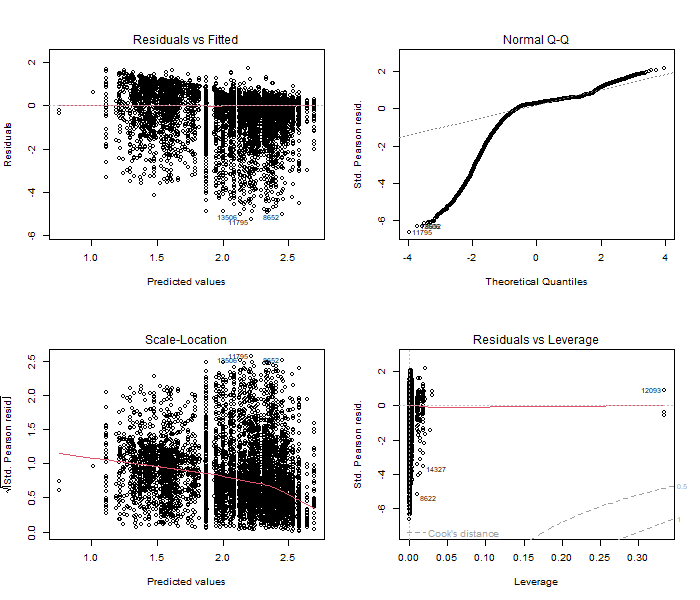
\includegraphics[width=1\textwidth,height=1\textheight]{C:/Users/Jason.Cope/Documents/Github/Sebastes_melanops_WA/Document/figures/index/GLMdiagnostics lognormal_Charter.png}
\caption{Diagnostic plots for the positive catch component of the lognormal delta-GLM model for the Washington charter boat Black Rockfish dataset. These plots are used to evaluate model fit (top left), assumptions of normality (top right), assumptions of constant variance (bottom left), and the presence of outliers (bottom right).\label{fig:charter-log-diags}}
\end{figure}

\pagebreak

\begin{figure}
\centering
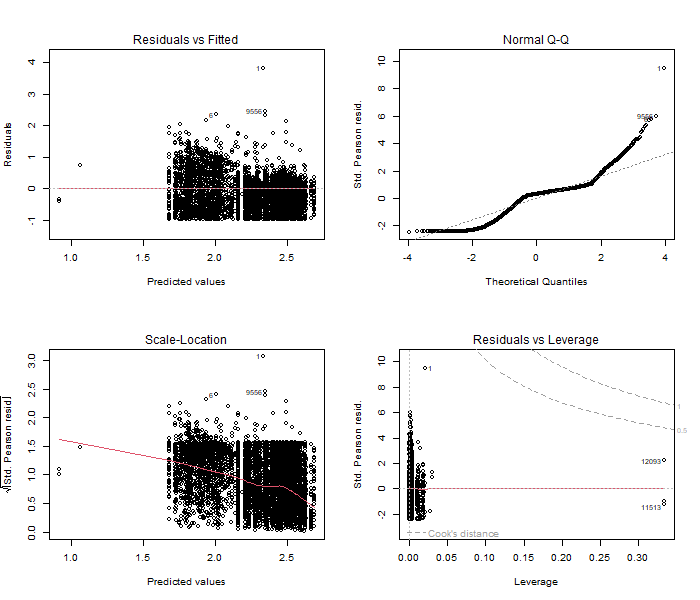
\includegraphics[width=1\textwidth,height=1\textheight]{C:/Users/Jason.Cope/Documents/Github/Sebastes_melanops_WA/Document/figures/index/GLMdiagnostics gamma_Charter.png}
\caption{Diagnostic plots for the positive catch component of the gamma delta-GLM model for the Washington charter boat Black Rockfish dataset. These plots are used to evaluate model fit (top left), assumptions of normality (top right), assumptions of constant variance (bottom left), and the presence of outliers (bottom right).\label{fig:charter-gam-diags}}
\end{figure}

\pagebreak

\begin{figure}
\centering
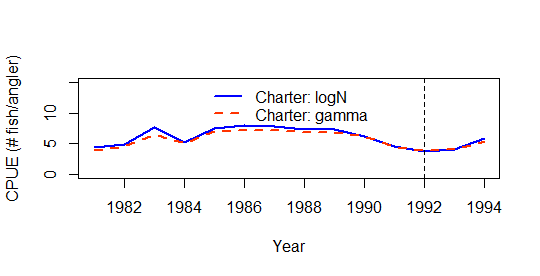
\includegraphics[width=1\textwidth,height=1\textheight]{C:/Users/Jason.Cope/Documents/Github/Sebastes_melanops_WA/Document/figures/index/WA_dockside_Charter94_Index.png}
\caption{Abundance indices for the WDFW charter boat CPUE analysis. Vertical lines are notable management actions (mainly bag limit changes). Colors and line type indicates different distributional treatments of the index.\label{fig:charter-index}}
\end{figure}

\pagebreak

\begin{figure}
\centering
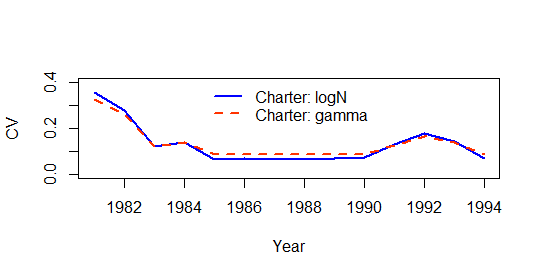
\includegraphics[width=1\textwidth,height=1\textheight]{C:/Users/Jason.Cope/Documents/Github/Sebastes_melanops_WA/Document/figures/index/WA_dockside_Charter94_CV.png}
\caption{Bootstrapped estimates of variation for each model of the Washington charter boat index.\label{fig:charter-CVs}}
\end{figure}

\pagebreak

\begin{figure}
\centering
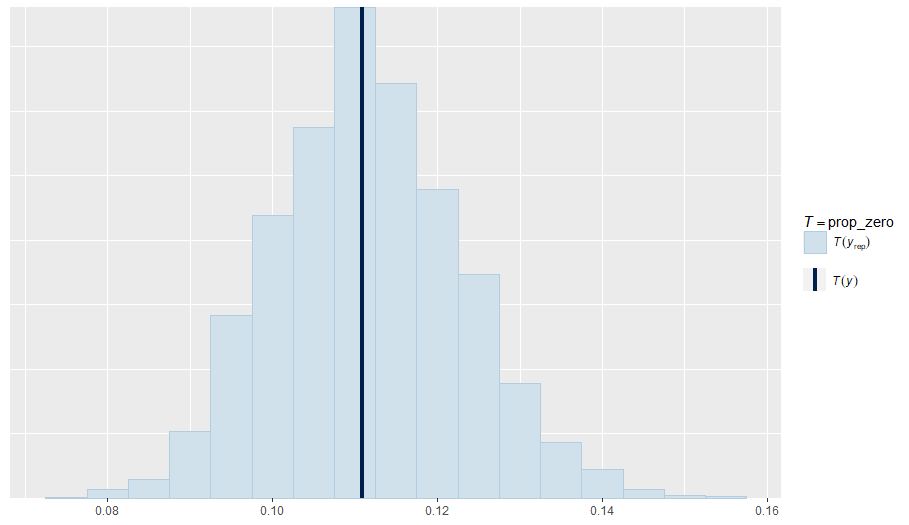
\includegraphics[width=1\textwidth,height=1\textheight]{C:/Users/Jason.Cope/Documents/Github/Sebastes_melanops_WA/Document/figures/index/ProportionZero_Tagging_1998_2018.png}
\caption{Estimated and observed proportion zero for the negative binomial tagging model.\label{fig:prop-zero-tag}}
\end{figure}

\pagebreak

\begin{figure}
\centering
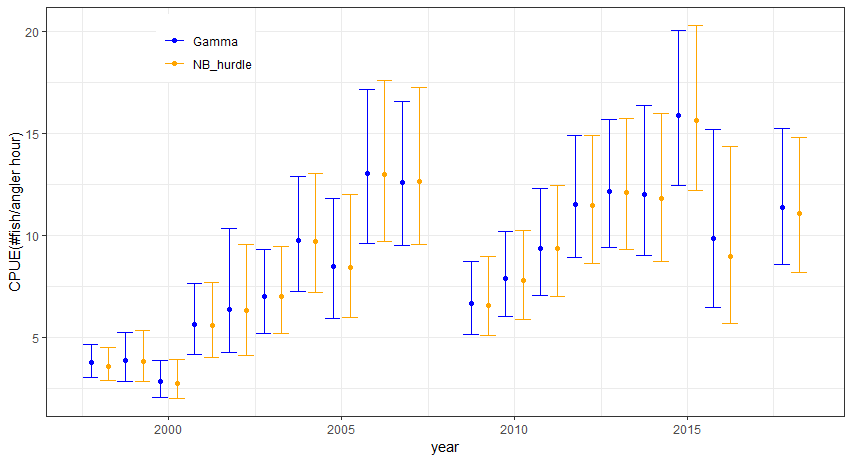
\includegraphics[width=1\textwidth,height=1\textheight]{C:/Users/Jason.Cope/Documents/Github/Sebastes_melanops_WA/Document/figures/index/HistoricTagging_1998_2018_Index.png}
\caption{Time series of the tagging index as produced by two separate standardization approaches. Gamma refers to the gamma distribution used in a delta glm model (as done in 2015). The NB\_hurdle refers to a Bayesian negative binomial hurdle model.\label{fig:tag-index}}
\end{figure}

\pagebreak

\begin{figure}
\centering
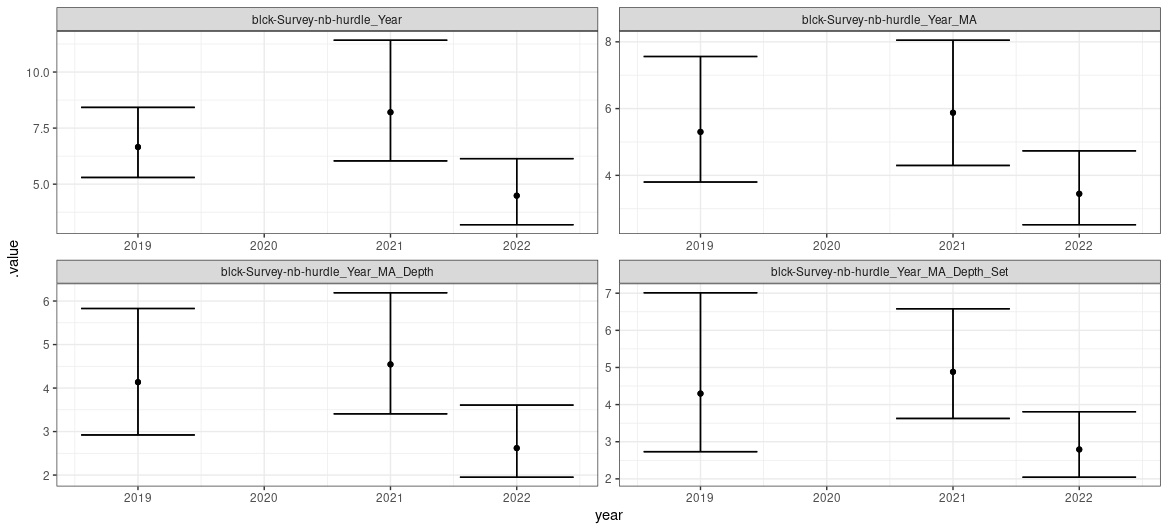
\includegraphics[width=1\textwidth,height=1\textheight]{C:/Users/Jason.Cope/Documents/Github/Sebastes_melanops_WA/Document/figures/index/Nearshore Survey_Hurdle.png}
\caption{Nearshore survey index and 95\% confidence intervals using different factors in the negative binomial hurdle model.\label{fig:model-sel-nearshore}}
\end{figure}

\pagebreak

\begin{figure}
\centering
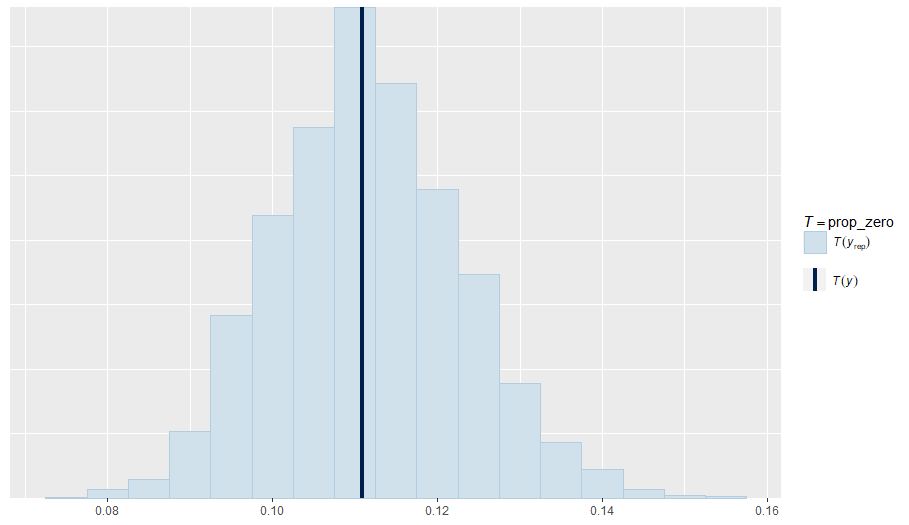
\includegraphics[width=1\textwidth,height=1\textheight]{C:/Users/Jason.Cope/Documents/Github/Sebastes_melanops_WA/Document/figures/index/ProportionZero_Tagging_1998_2018.png}
\caption{Estimated and observed proportion zero for the negative binomial nearshore survey model.\label{fig:prop-zero-nearshore}}
\end{figure}

\pagebreak

\begin{figure}
\centering
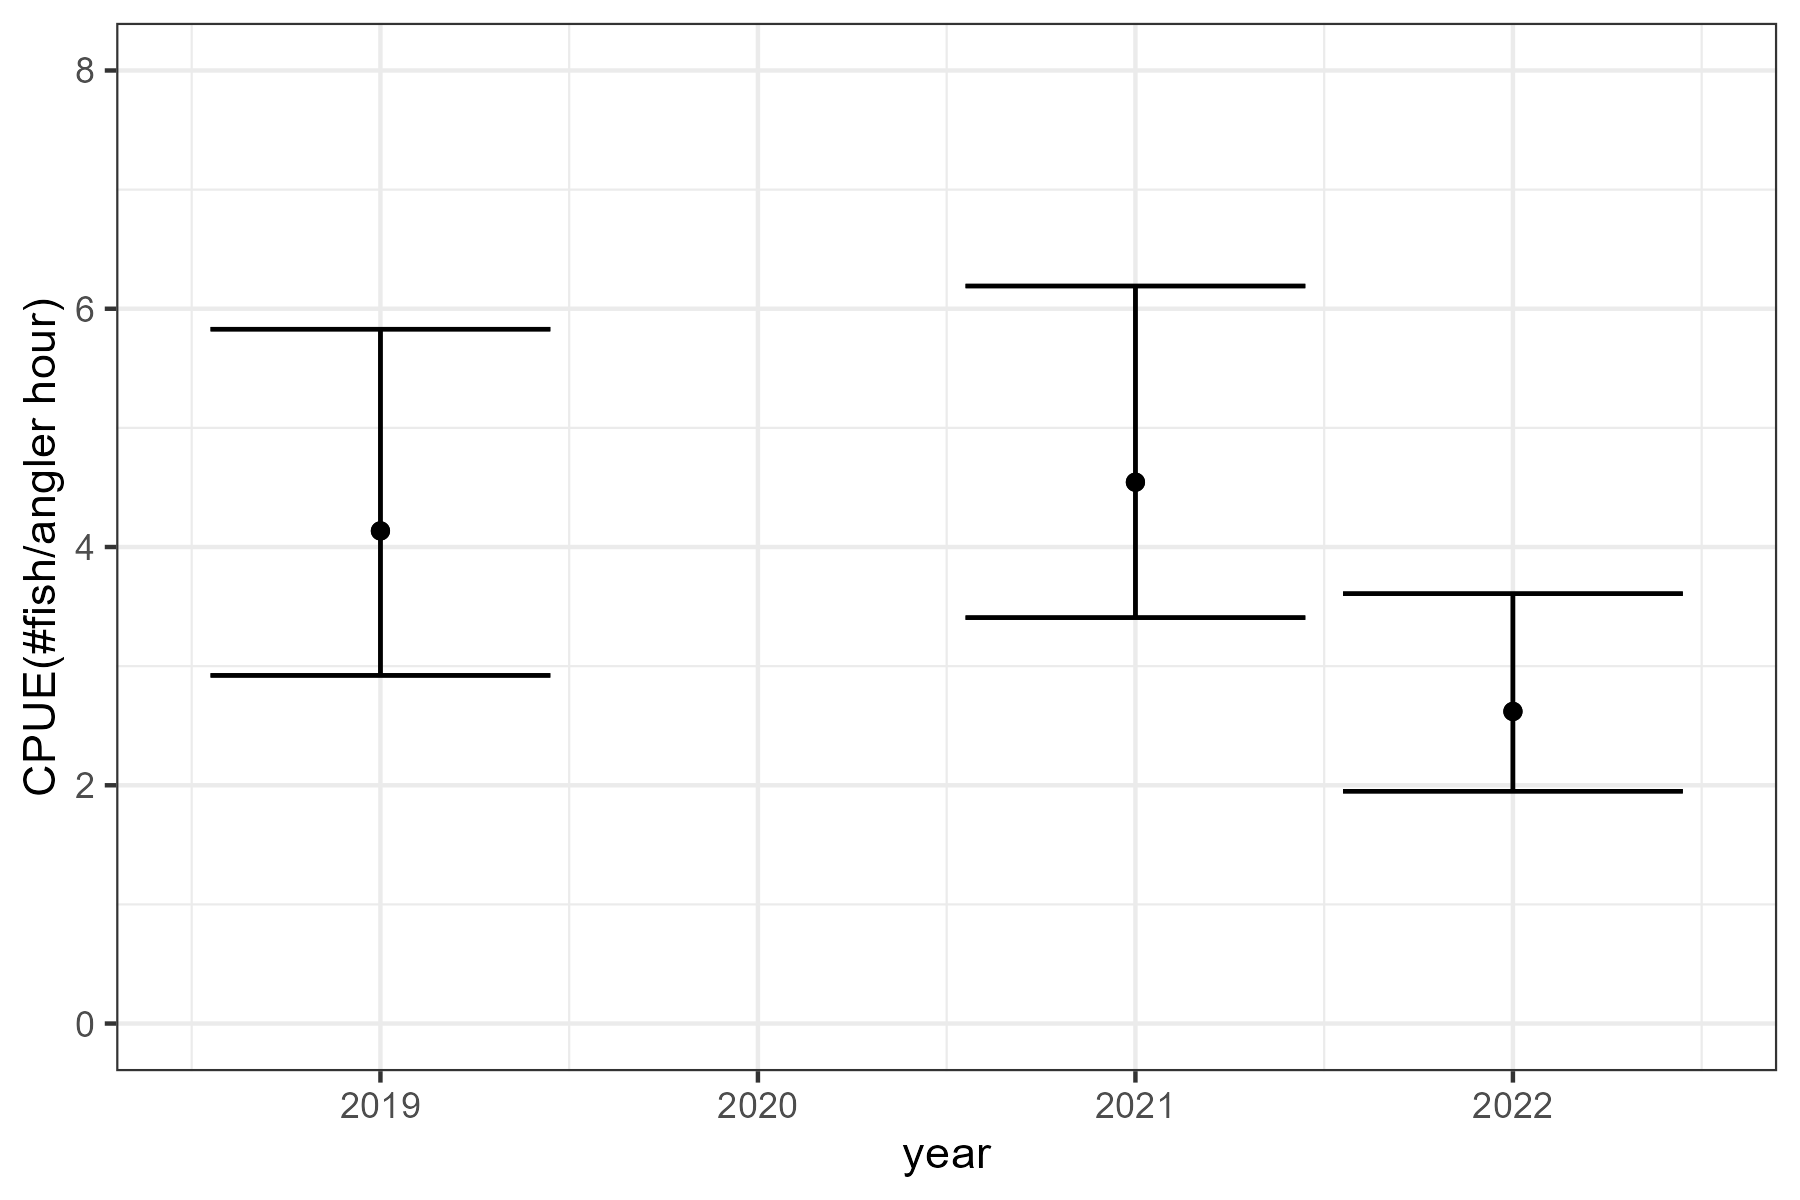
\includegraphics[width=1\textwidth,height=1\textheight]{C:/Users/Jason.Cope/Documents/Github/Sebastes_melanops_WA/Document/figures/index/Hurdles_NearshoreSurveyIndex.png}
\caption{Nearshore index time series with 95\% confidence intervals.\label{fig:nearshore-index}}
\end{figure}

\pagebreak

\begin{figure}
\centering
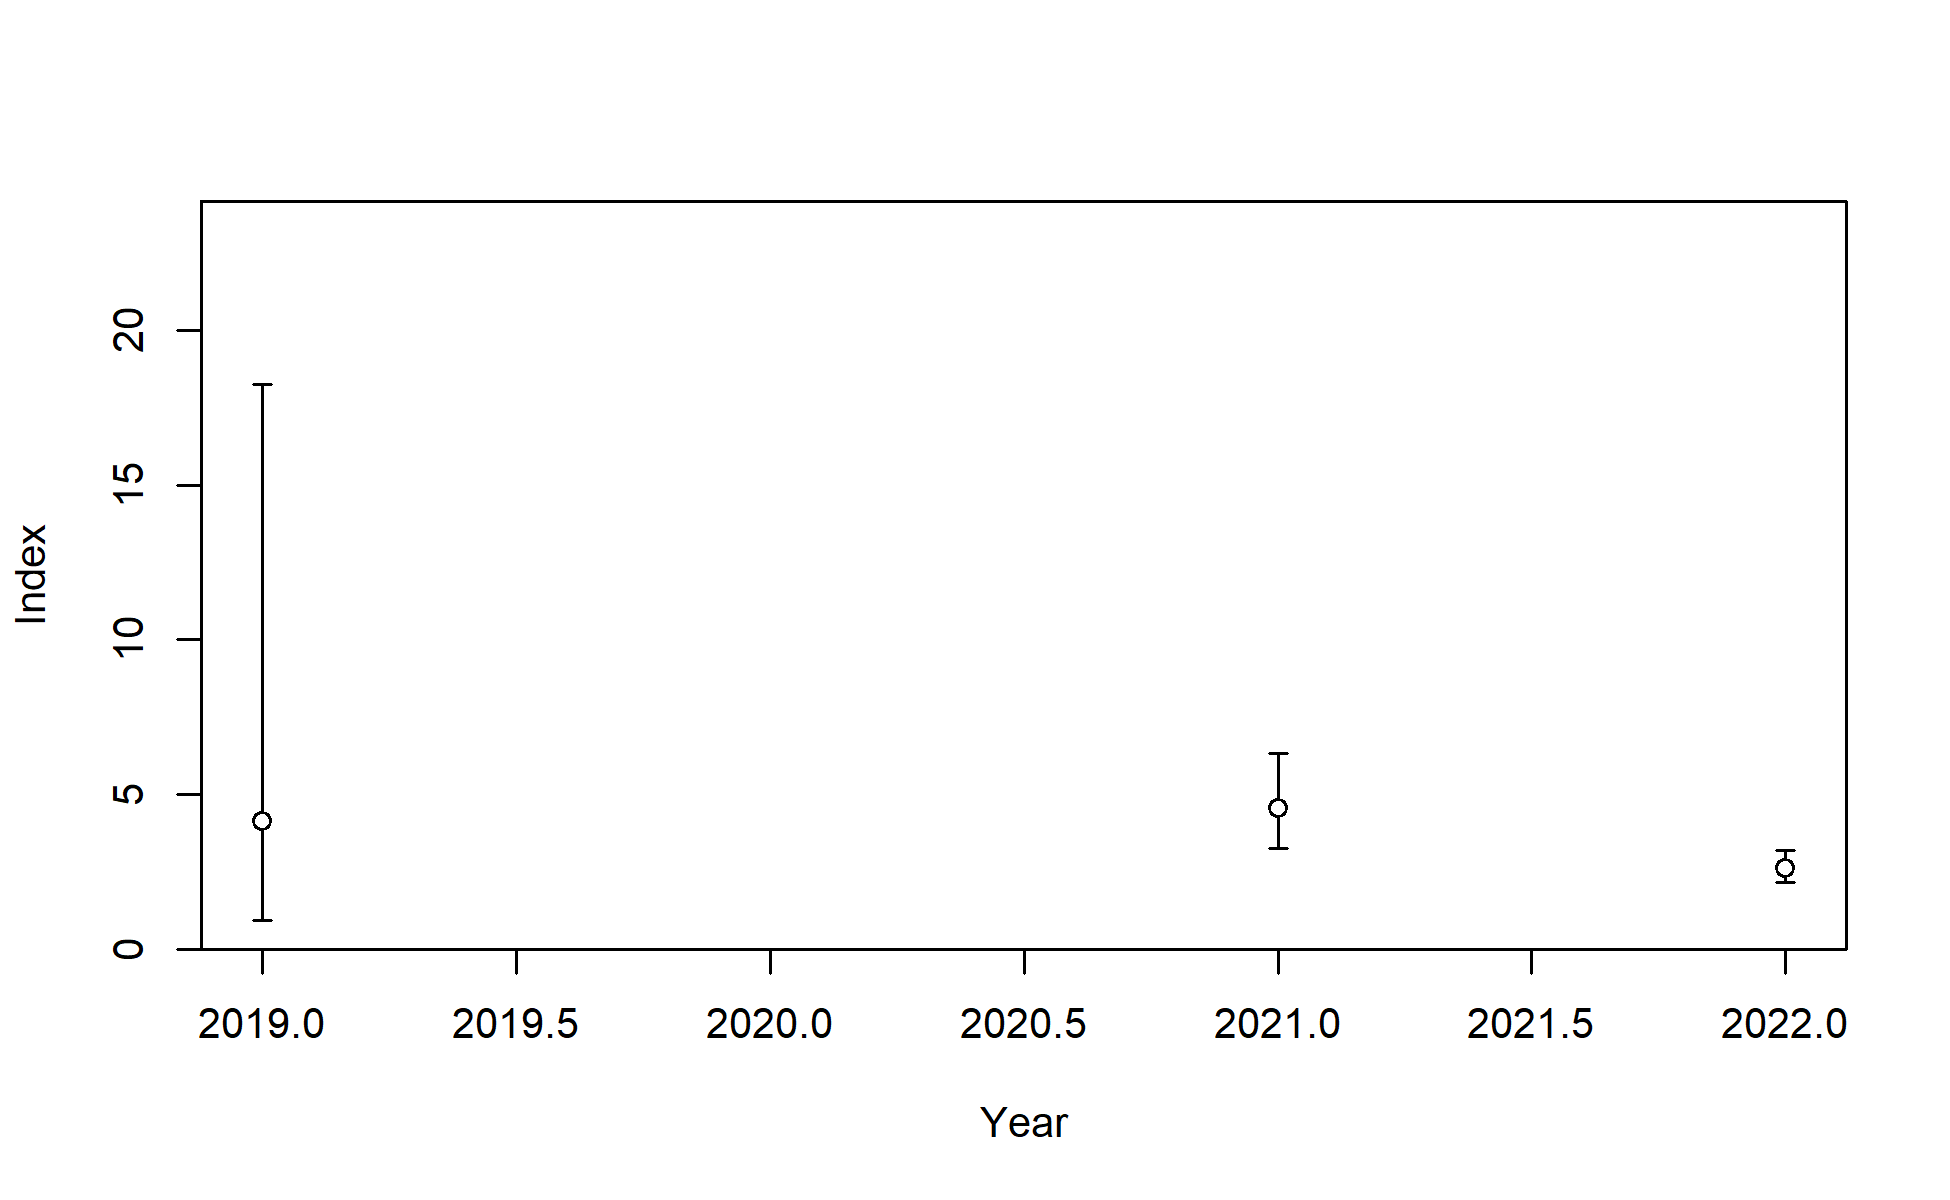
\includegraphics[width=1\textwidth,height=1\textheight]{C:/Users/Jason.Cope/Documents/Github/Sebastes_melanops_WA/Document/models/Reference model/plots/index1_cpuedata_Nearshore_survey.png}
\caption{Nearshore index time series.\label{fig:nearshore-index}}
\end{figure}

\pagebreak

\hypertarget{biology}{%
\subsection{Biology}\label{biology}}

\begin{figure}
\centering
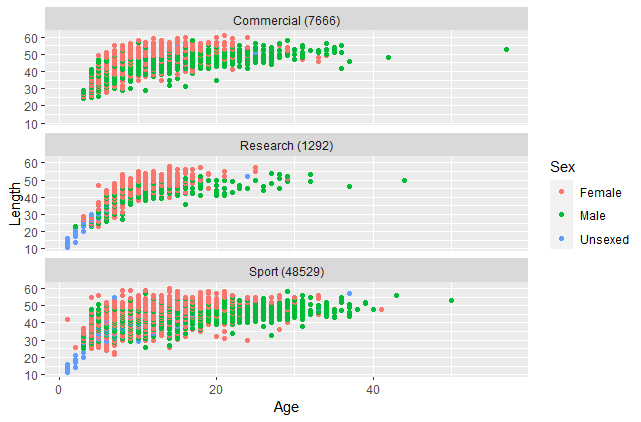
\includegraphics[width=1\textwidth,height=1\textheight]{C:/Users/Jason.Cope/Documents/Github/Sebastes_melanops_WA/Document/figures/biology_plots/WA_AG_Source_Sex.png}
\caption{Observed length-at-age by data source and sex.\label{fig:len-age-data-sex}}
\end{figure}

\pagebreak

\begin{figure}
\centering
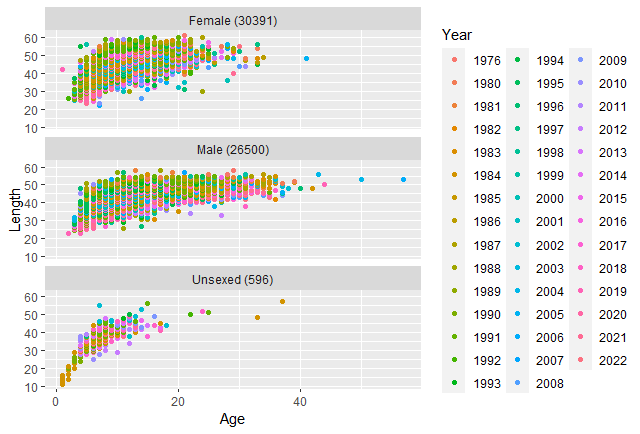
\includegraphics[width=1\textwidth,height=1\textheight]{C:/Users/Jason.Cope/Documents/Github/Sebastes_melanops_WA/Document/figures/biology_plots/WA_AG_Sex_Year.png}
\caption{Observed length-at-age by sex and year. Total samples are indicated in parentheses.\label{fig:len-age-sex-year}}
\end{figure}

\pagebreak

\begin{figure}
\centering
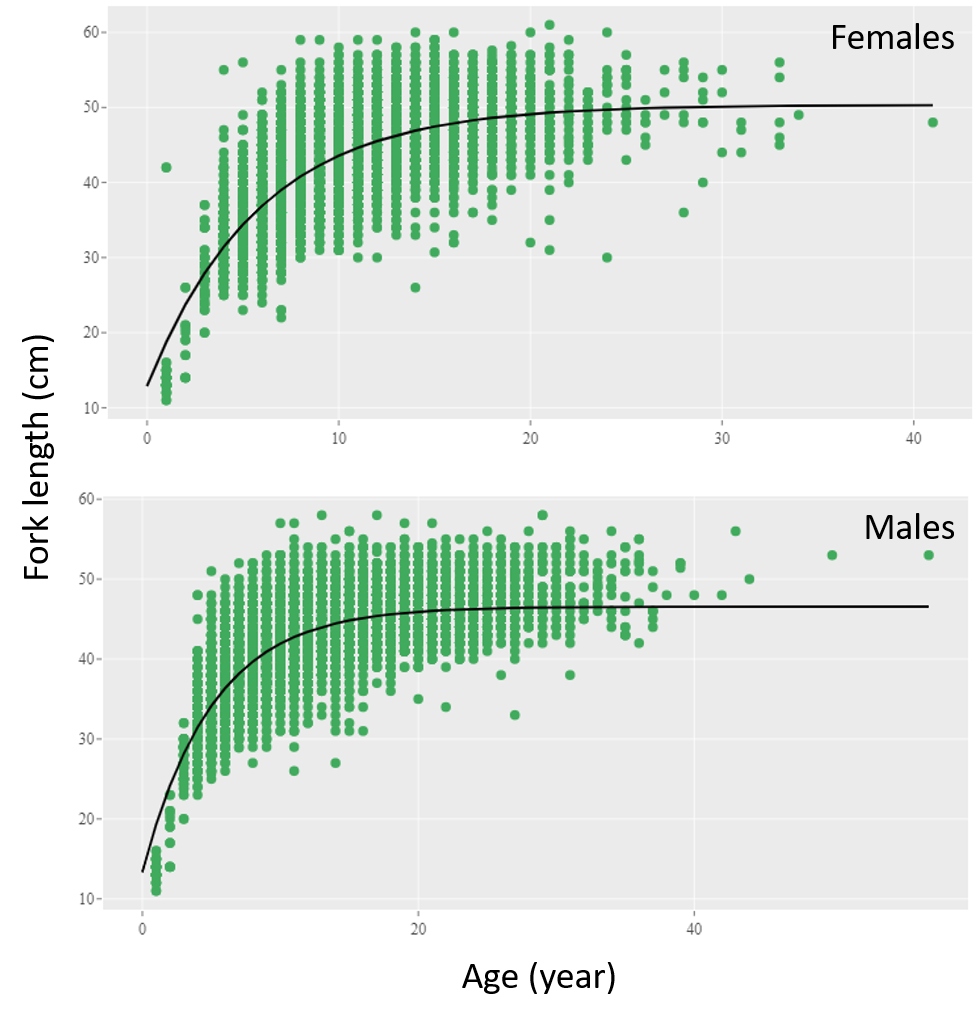
\includegraphics[width=1\textwidth,height=1\textheight]{C:/Users/Jason.Cope/Documents/Github/Sebastes_melanops_WA/Document/figures/biology_plots/WA_VBGF_fit.png}
\caption{External fits to the observed length-at-age by sex.\label{fig:len-age-fit}}
\end{figure}

\pagebreak

\begin{figure}
\centering
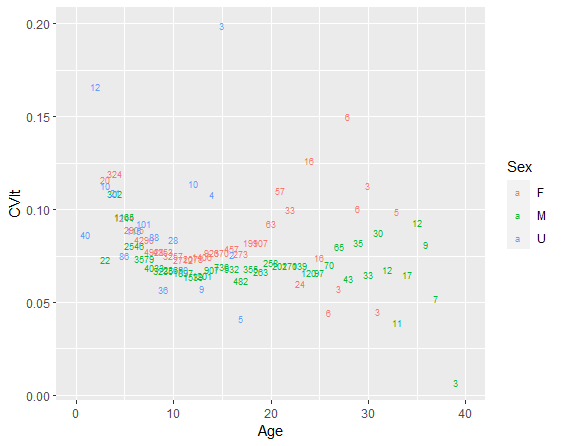
\includegraphics[width=1\textwidth,height=1\textheight]{C:/Users/Jason.Cope/Documents/Github/Sebastes_melanops_WA/Document/figures/biology_plots/WA_CV_Sex_plot.png}
\caption{Coefficient of variation of length by age by sex. Numbers indicate samples by age and colors indicate sex.\label{fig:cv-lt-age}}
\end{figure}

\pagebreak

\begin{figure}
\centering
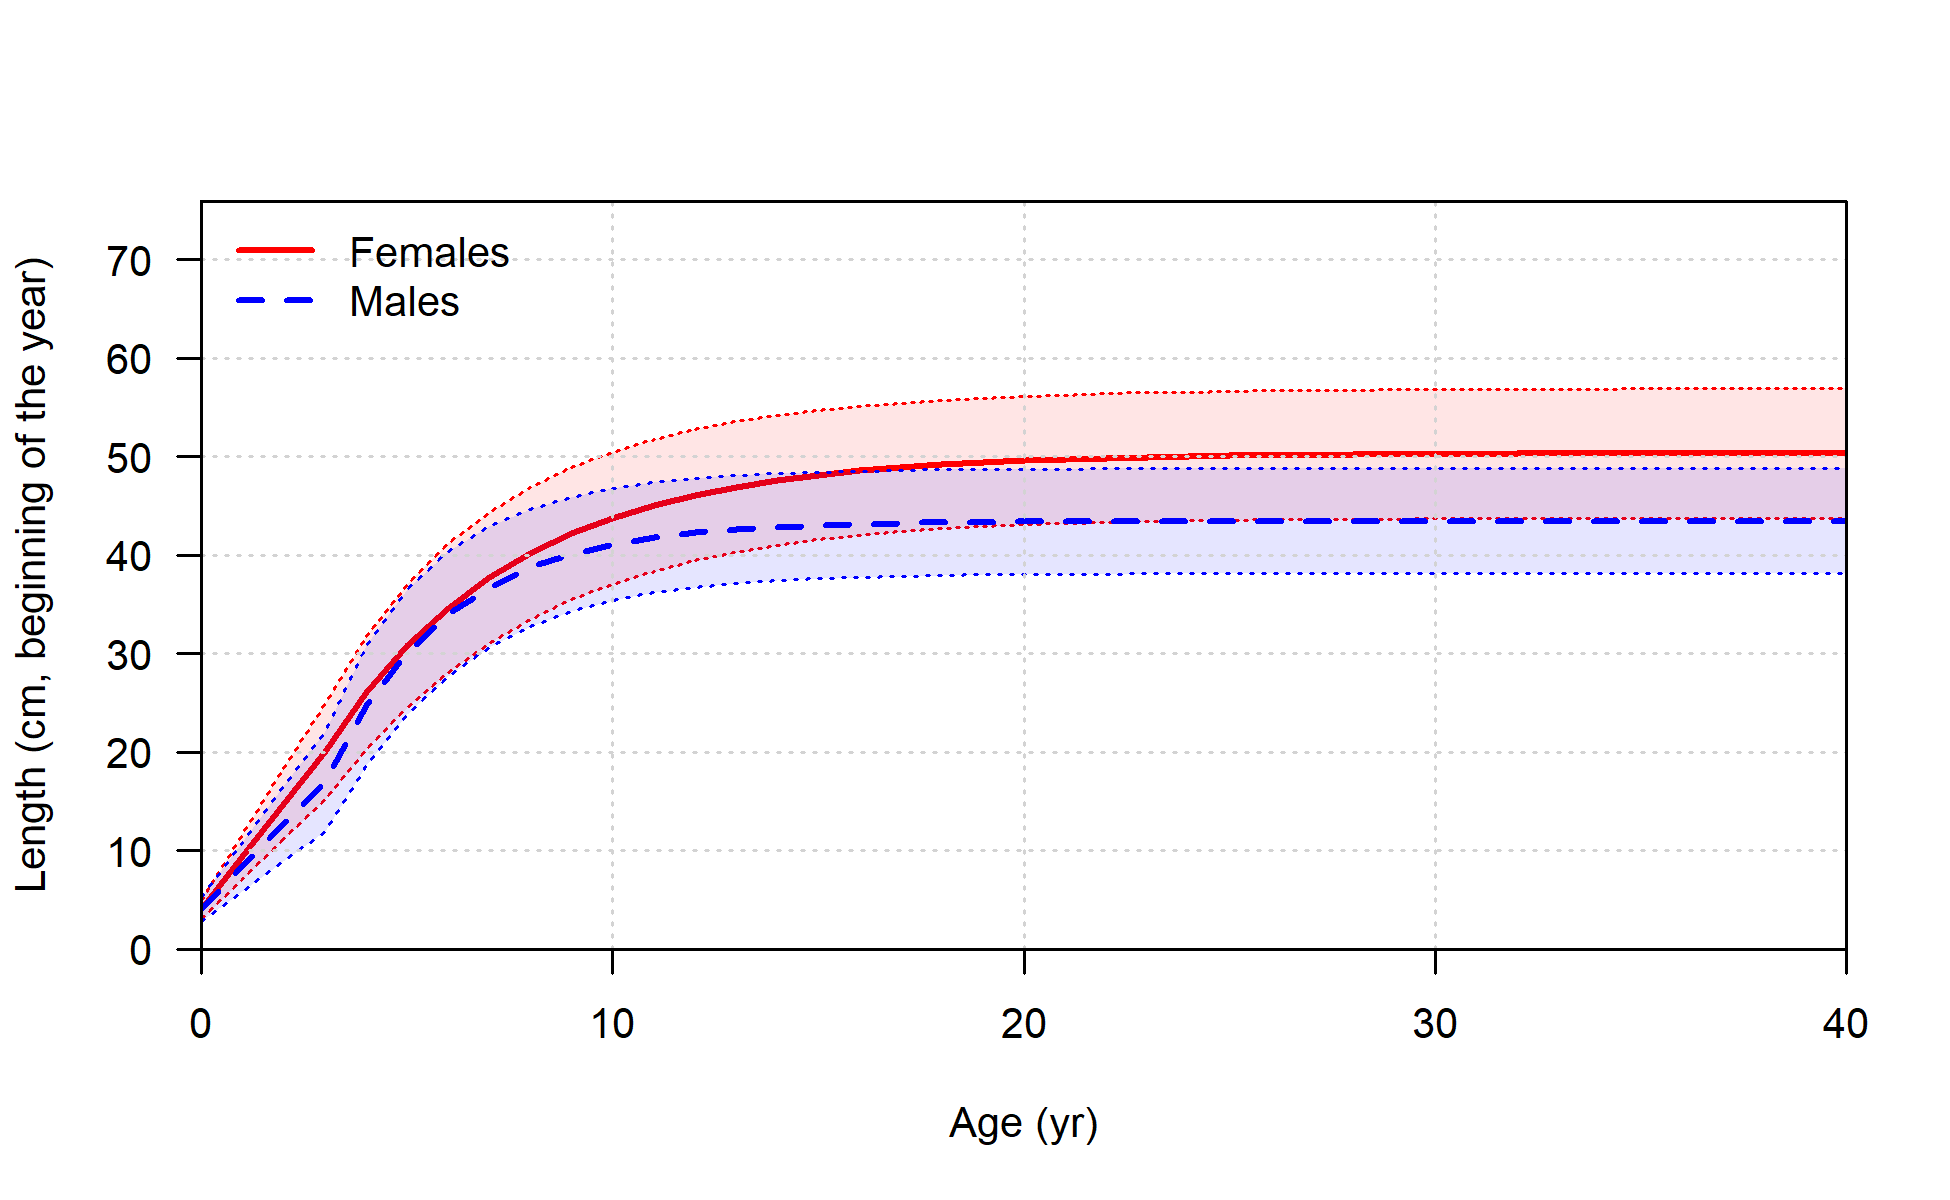
\includegraphics[width=1\textwidth,height=1\textheight]{C:/Users/Jason.Cope/Documents/Github/Sebastes_melanops_WA/Document/models/Reference model/plots/bio1_sizeatage.png}
\caption{Model estimated length-at-age. Shaded area indicates 95 percent distribution of length-at-age around the estimated growth curve.\label{fig:len-age-ss}}
\end{figure}

\clearpage

\begin{figure}
\centering
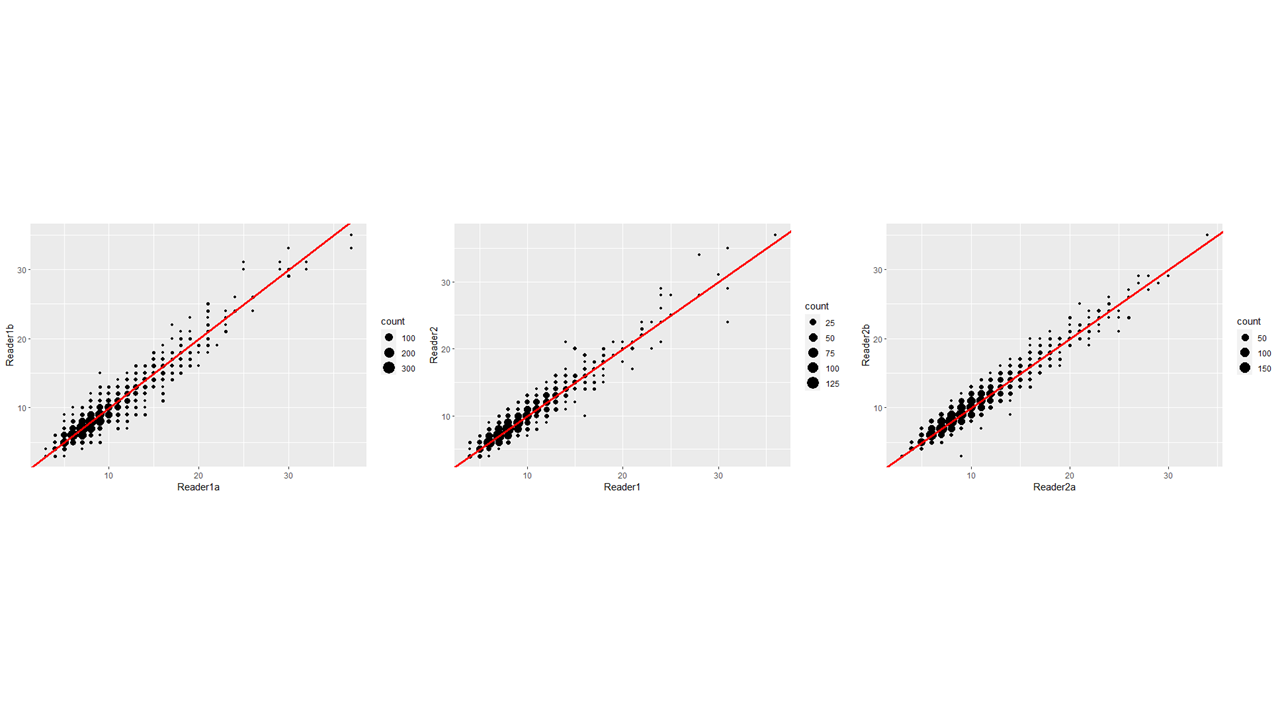
\includegraphics[width=1\textwidth,height=1\textheight]{C:/Users/Jason.Cope/Documents/Github/Sebastes_melanops_WA/Document/figures/biology_plots/Age1_1plots.png}
\caption{Ageing bias plots by reader comparisons.\label{fig:a1-bias}}
\end{figure}

\pagebreak

\begin{figure}
\centering
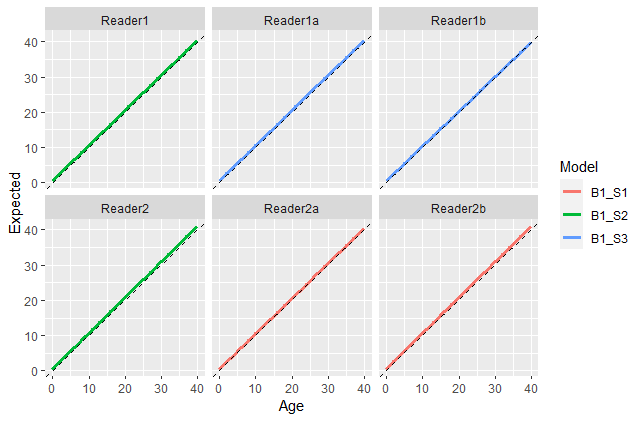
\includegraphics[width=1\textwidth,height=1\textheight]{C:/Users/Jason.Cope/Documents/Github/Sebastes_melanops_WA/Document/figures/biology_plots/WA_Reader_Bias_plot.png}
\caption{Estimated bias relationships for each considered matrix. Reader 1 is always considered unbiased. Reader 1a and 1b is an intra-reader comparison. B refers to the bias type and S refers to the imprecision type in the model selection for the ageing error matrix.\label{fig:age-error-bias}}
\end{figure}

\pagebreak

\begin{figure}
\centering
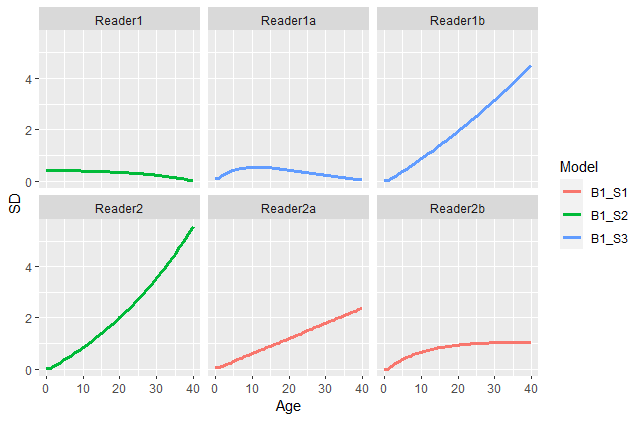
\includegraphics[width=1\textwidth,height=1\textheight]{C:/Users/Jason.Cope/Documents/Github/Sebastes_melanops_WA/Document/figures/biology_plots/WA_Reader_SD_plot.png}
\caption{Ageing error matrix standard deviation (SD) values by comparison. B refers to the bias type and S refers to the imprecision type in the model selection for the ageing error matrix.\label{fig:age-error-sd}}
\end{figure}

\pagebreak

\begin{figure}
\centering
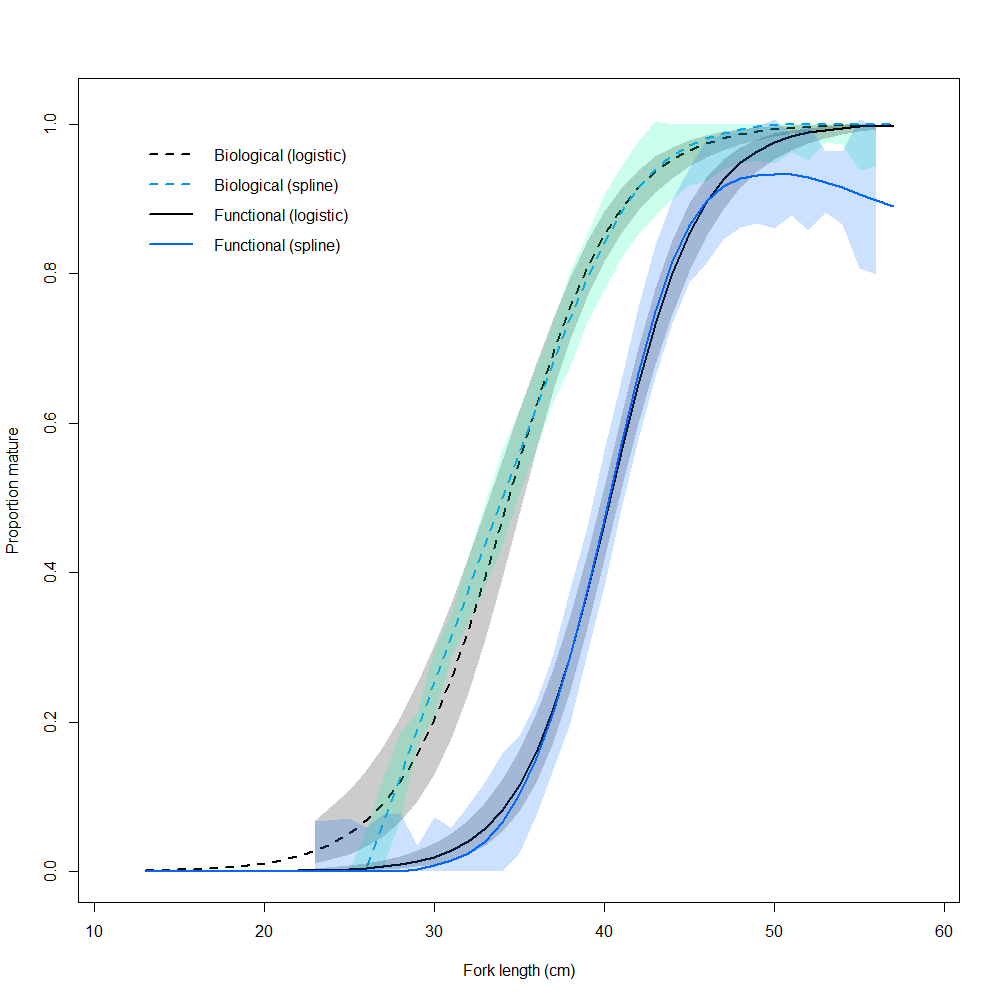
\includegraphics[width=1\textwidth,height=1\textheight]{C:/Users/Jason.Cope/Documents/Github/Sebastes_melanops_WA/Document/figures/biology_plots/Fig1_bio_and_func_color.png}
\caption{Biological and functional maturity ogives. Biological maturity ogives are represented by the dashed lines (logistic regression and 95\% CI is grey, flexible spline and 95\% CI is light green). Functional maturity ogives are represented by the solid lines (logistic regression and 95\% CI is grey, flexible spline and 95\% CI is light blue).\label{fig:bio-fxn-mat-color}}
\end{figure}

\pagebreak

\begin{figure}
\centering
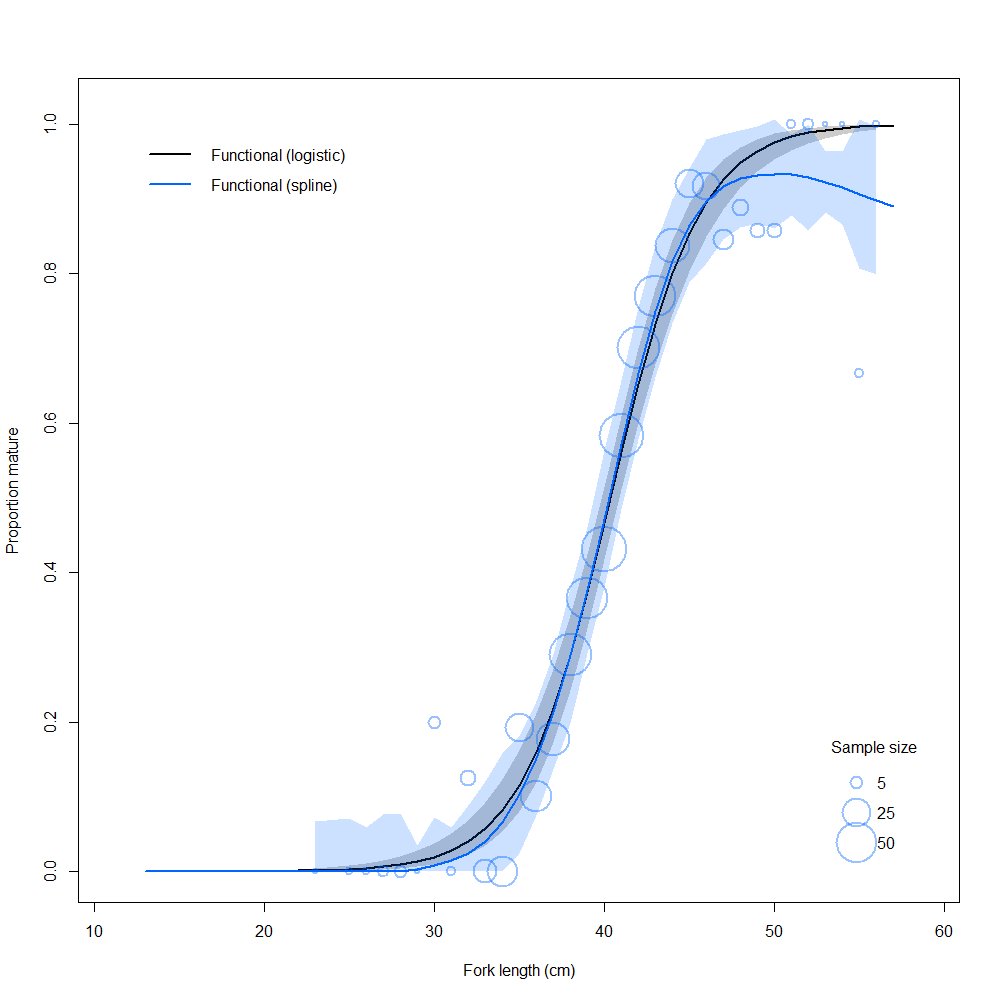
\includegraphics[width=1\textwidth,height=1\textheight]{C:/Users/Jason.Cope/Documents/Github/Sebastes_melanops_WA/Document/figures/biology_plots/Fig2_func_samplesize_color.png}
\caption{Functional maturity ogives and sample size. Functional maturity ogives are represented by the solid lines (logistic regression and 95\% CI is grey, flexible spline and 95\% CI is light blue) and sample size is denoted by the size of the bubbles).\label{fig:fxn-spline-mat-color}}
\end{figure}

\pagebreak

\begin{figure}
\centering
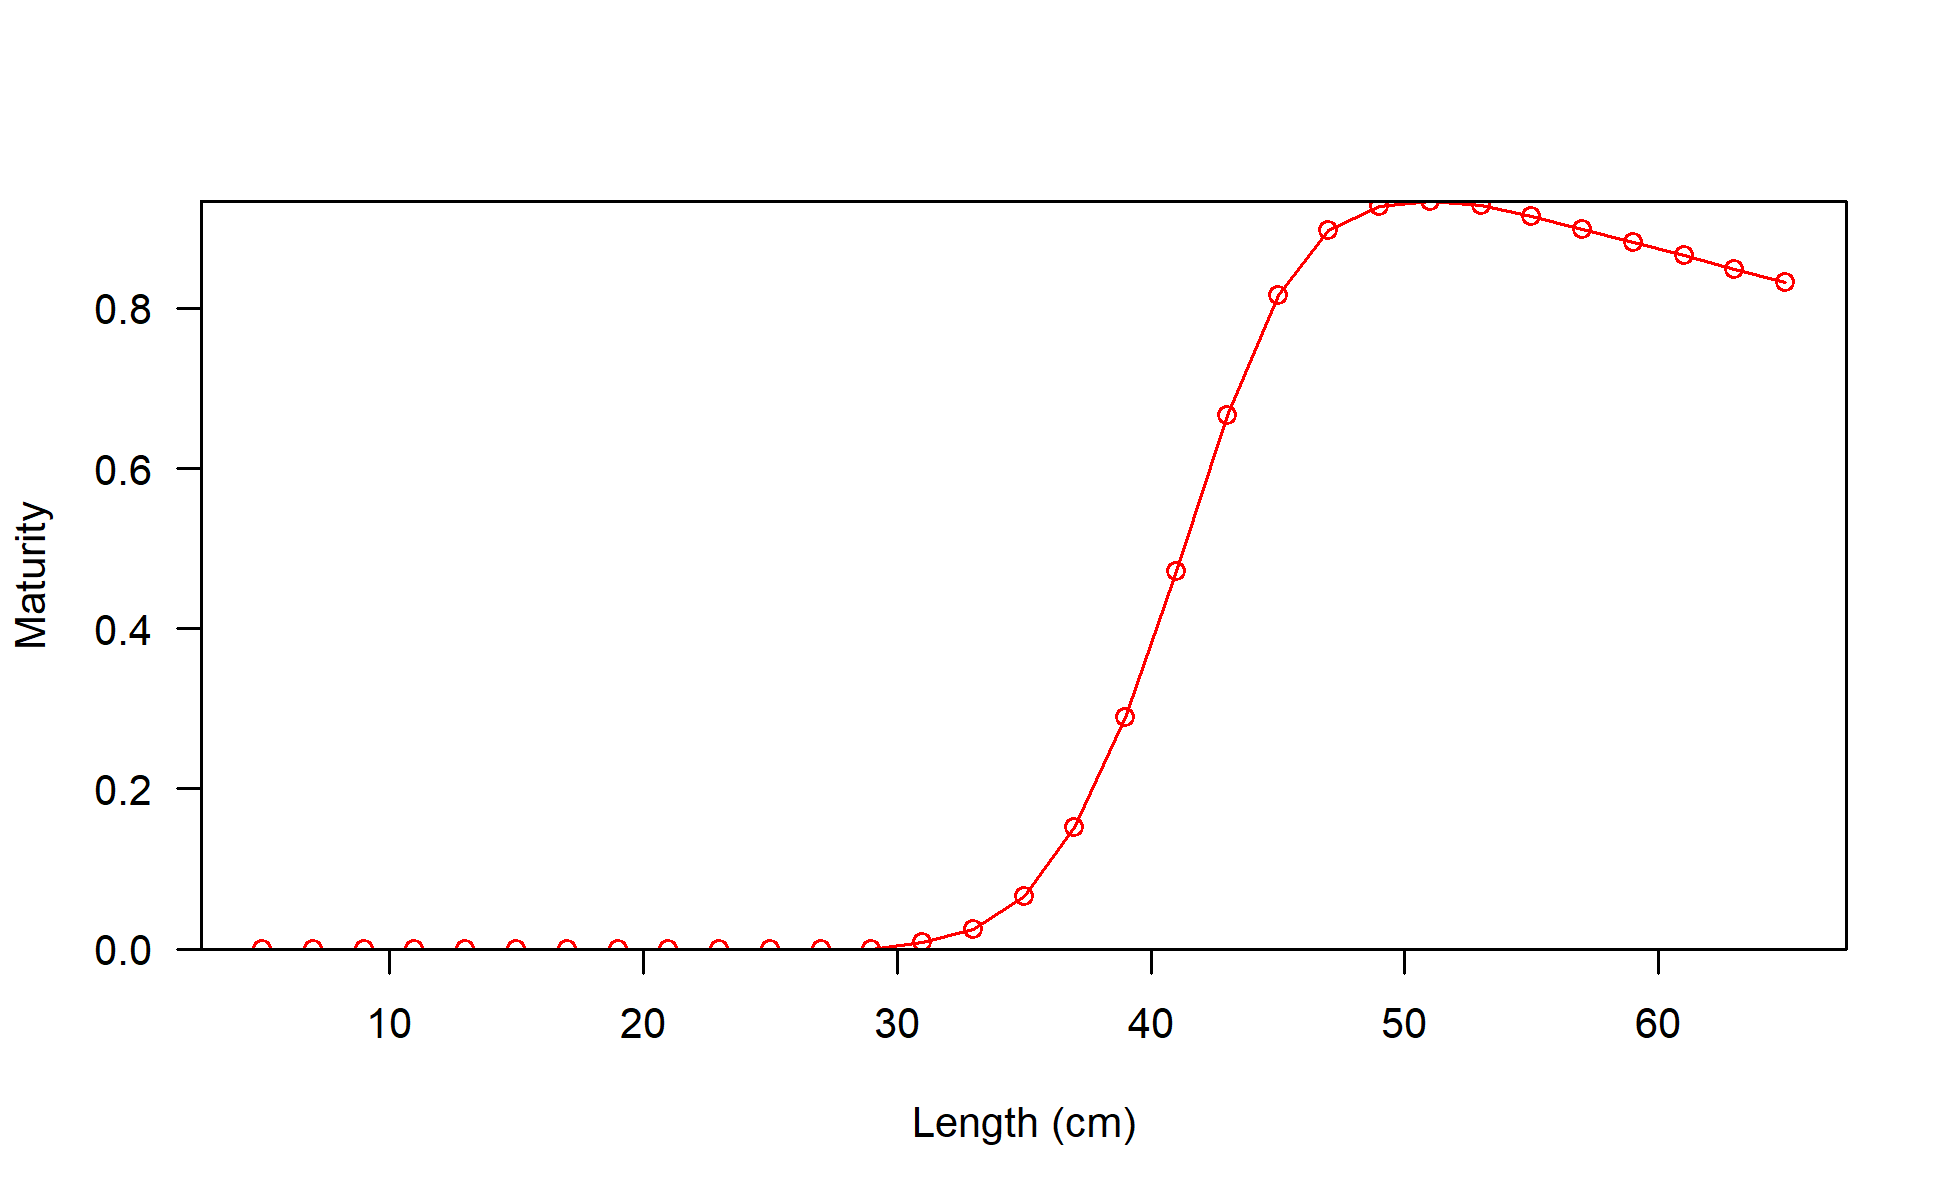
\includegraphics[width=1\textwidth,height=1\textheight]{C:/Users/Jason.Cope/Documents/Github/Sebastes_melanops_WA/Document/models/Reference model/plots/bio6_maturity.png}
\caption{Maturity as a function of length (cm).\label{fig:maturity}}
\end{figure}

\pagebreak

\begin{figure}
\centering
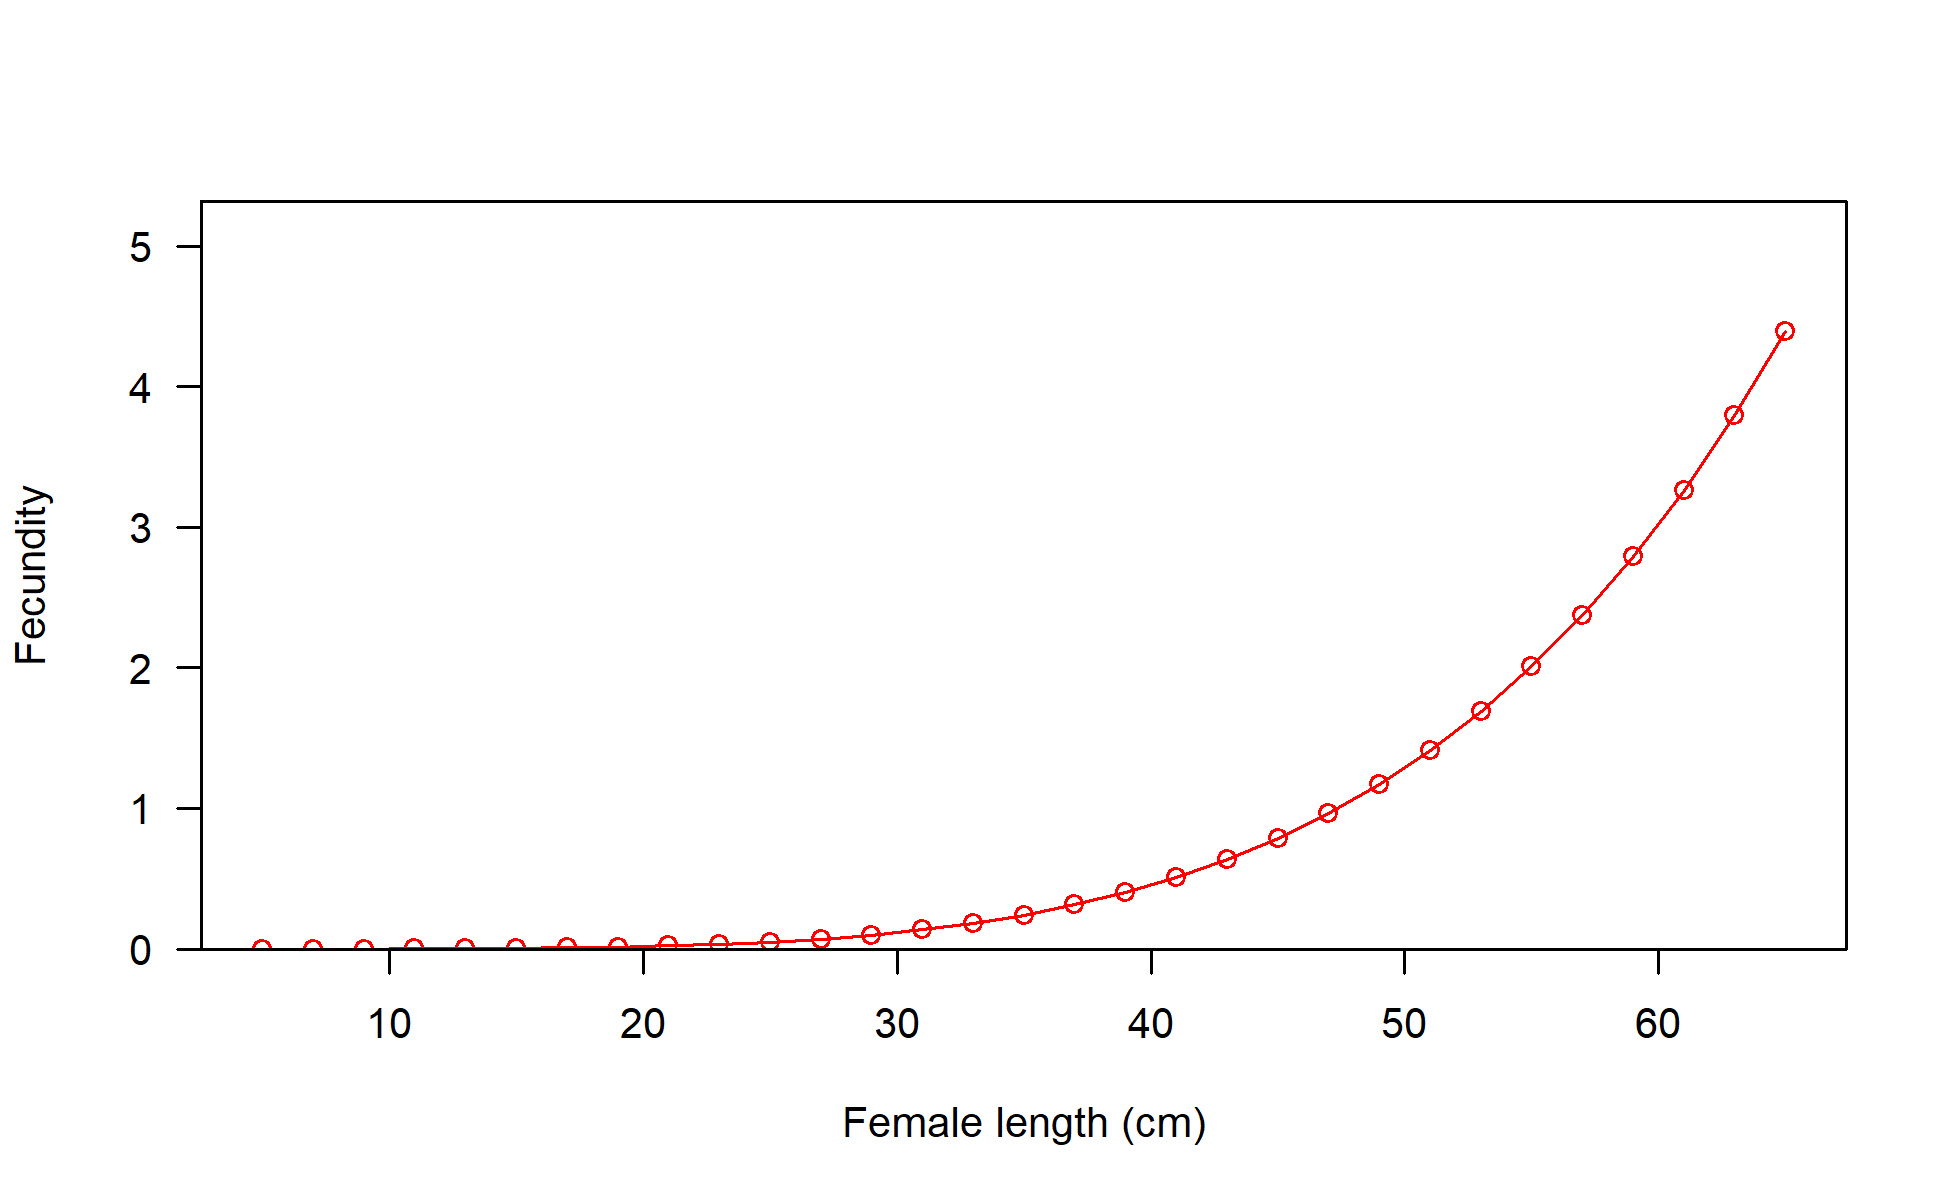
\includegraphics[width=1\textwidth,height=1\textheight]{C:/Users/Jason.Cope/Documents/Github/Sebastes_melanops_WA/Document/models/Reference model/plots/bio9_fecundity_len.png}
\caption{Fecundity (kg) as a function of length (cm).\label{fig:fecundity}}
\end{figure}

\pagebreak

\begin{figure}
\centering
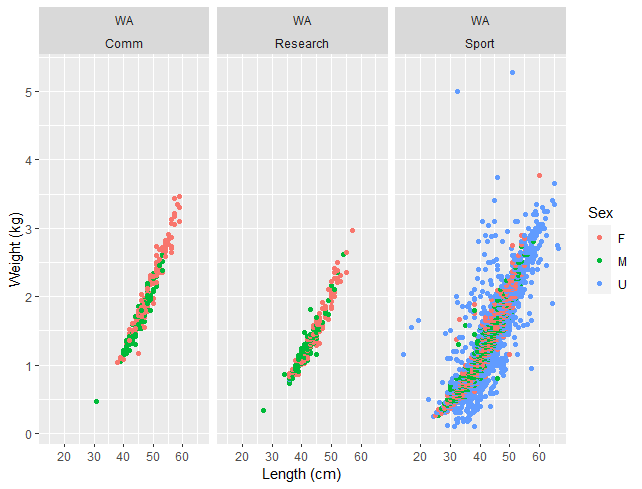
\includegraphics[width=1\textwidth,height=1\textheight]{C:/Users/Jason.Cope/Documents/Github/Sebastes_melanops_WA/Document/figures/biology_plots/LW_WA_State_Source_Sex.png}
\caption{Sex-specific length (cm)-weight (kg) data for Black Rockfish samples by source.\label{fig:len-weight-data}}
\end{figure}

\pagebreak

\begin{figure}
\centering
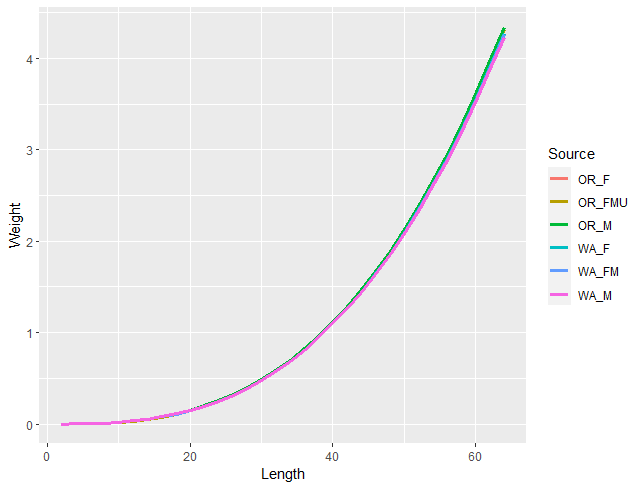
\includegraphics[width=1\textwidth,height=1\textheight]{C:/Users/Jason.Cope/Documents/Github/Sebastes_melanops_WA/Document/figures/biology_plots/LW_lines_States_Sex.png}
\caption{Sex-specific length (cm)-weight (kg) estimated power function relationships. Washington state estimate relationships are also provided for comparison.\label{fig:len-weight-or-wa}}
\end{figure}

\clearpage

\hypertarget{modeling}{%
\subsection{Modeling}\label{modeling}}

\hypertarget{bridging}{%
\subsubsection{Bridging}\label{bridging}}

\begin{figure}
\centering
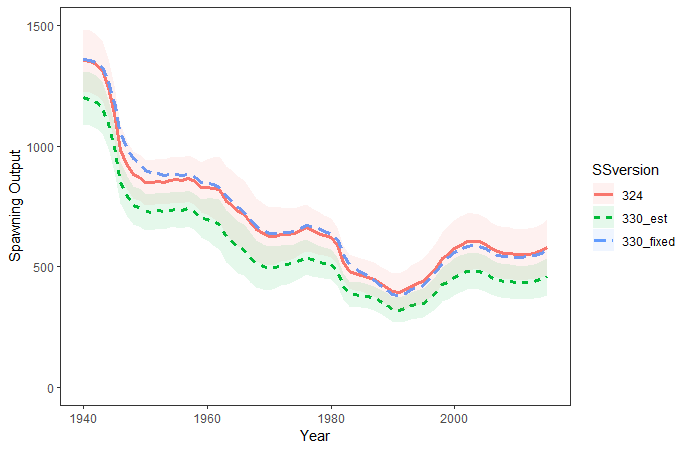
\includegraphics[width=1\textwidth,height=1\textheight]{C:/Users/Jason.Cope/Documents/Github/Sebastes_melanops_WA/Document/figures/Bridge/WA_SB_comp_plot.png}
\caption{Comparison of spawning output for Black Rockfish in waters off of Washington between Stock Synthesis versions 3.24 and 3.30. Uncertainty envelops are 95\% confidence intervals.\label{fig:ssb_bridge_comps}}
\end{figure}

\pagebreak

\begin{figure}
\centering
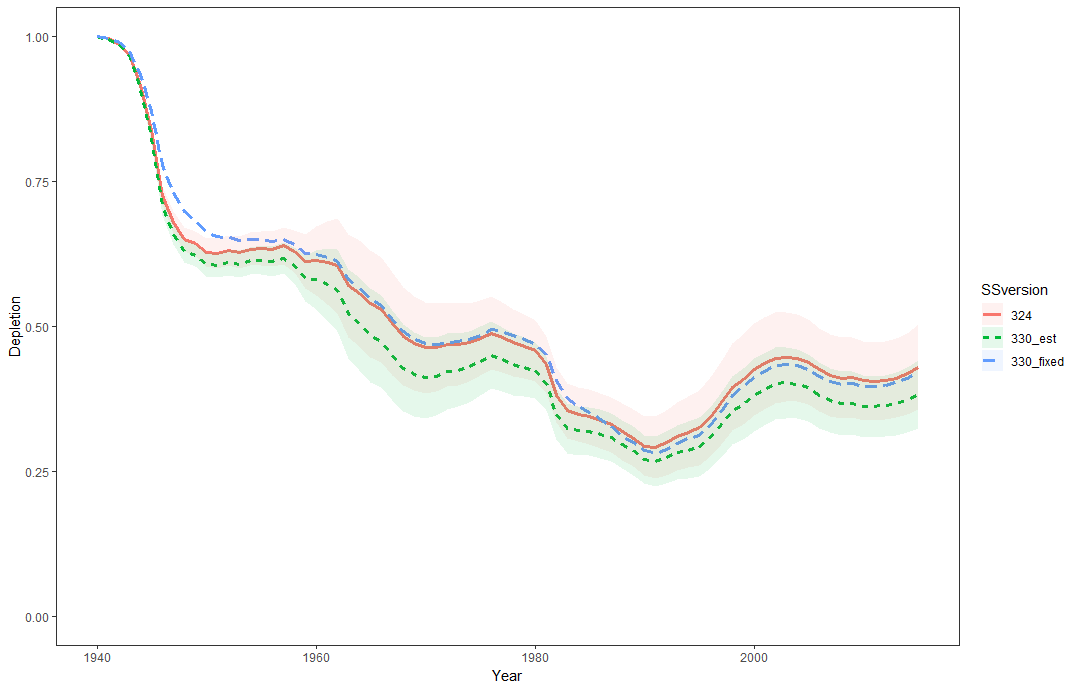
\includegraphics[width=1\textwidth,height=1\textheight]{C:/Users/Jason.Cope/Documents/Github/Sebastes_melanops_WA/Document/figures/Bridge/WA_Dep_comp_plot.png}
\caption{Comparison of spawning output for Black Rockfish in waters off of Washington between Stock Synthesis versions 3.24 and 3.30. Uncertainty envelops are 95\% confidence intervals.\label{fig:deps_bridge_comps}}
\end{figure}

\pagebreak

\begin{figure}
\centering
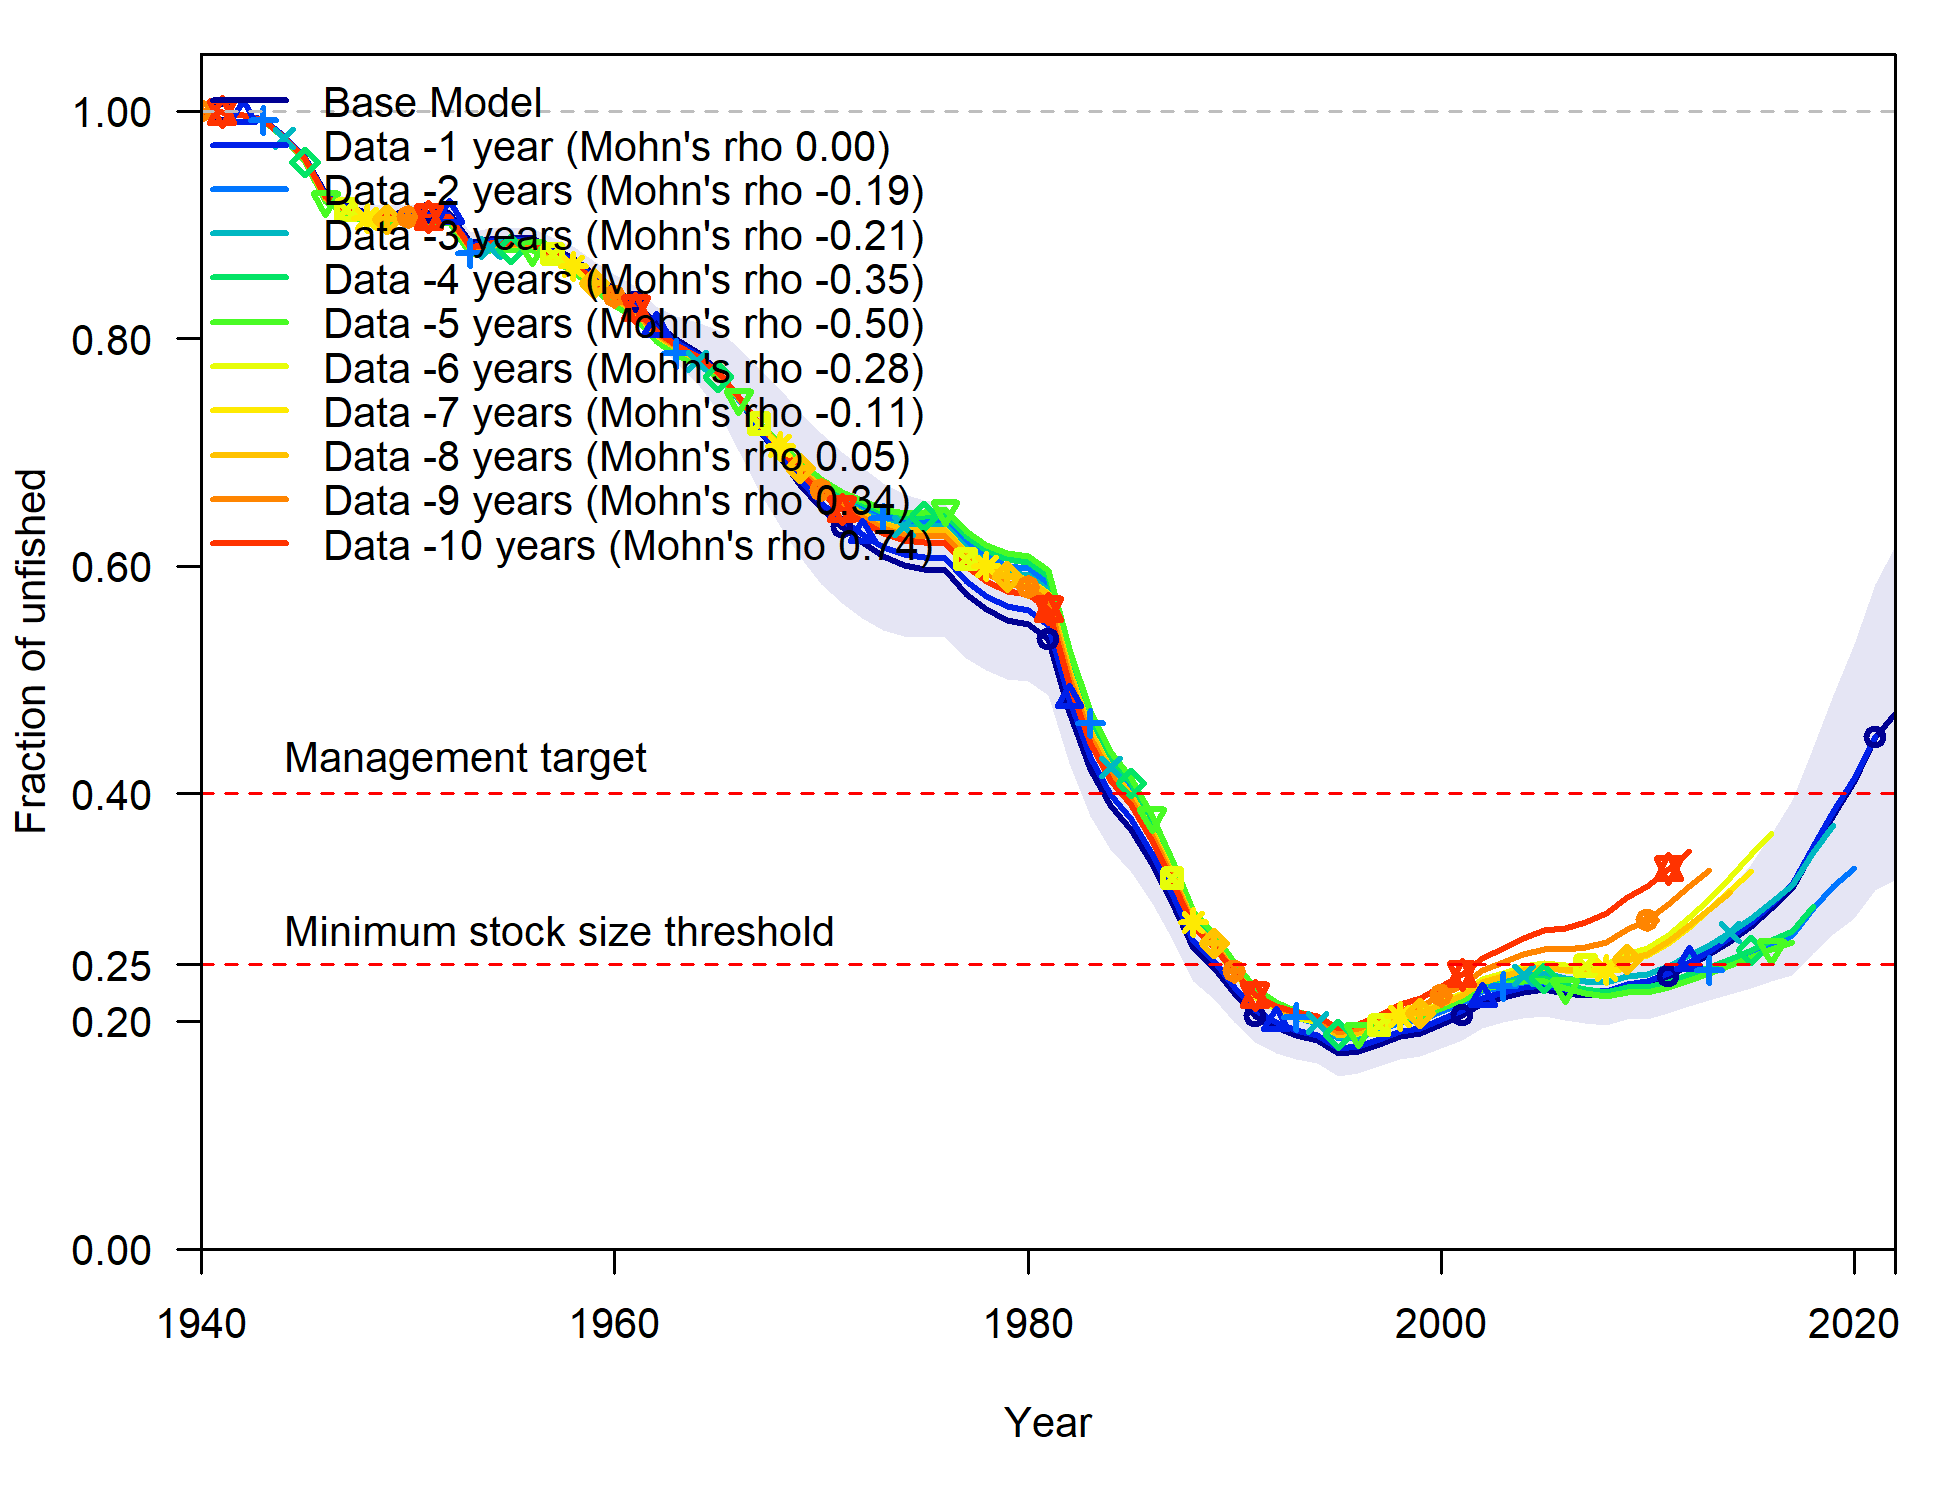
\includegraphics[width=1\textwidth,height=1\textheight]{C:/Users/Jason.Cope/Documents/Github/Sebastes_melanops_WA/Document/figures/modbuild/Mod build stock status/compare4_Bratio_uncertainty.png}
\caption{Relative spawning output time series by data treatment compared to the reference model. Missing scenarios mean the spawning output was too large to show.\label{fig:modbuild-data-depl}}
\end{figure}

\begin{figure}
\centering
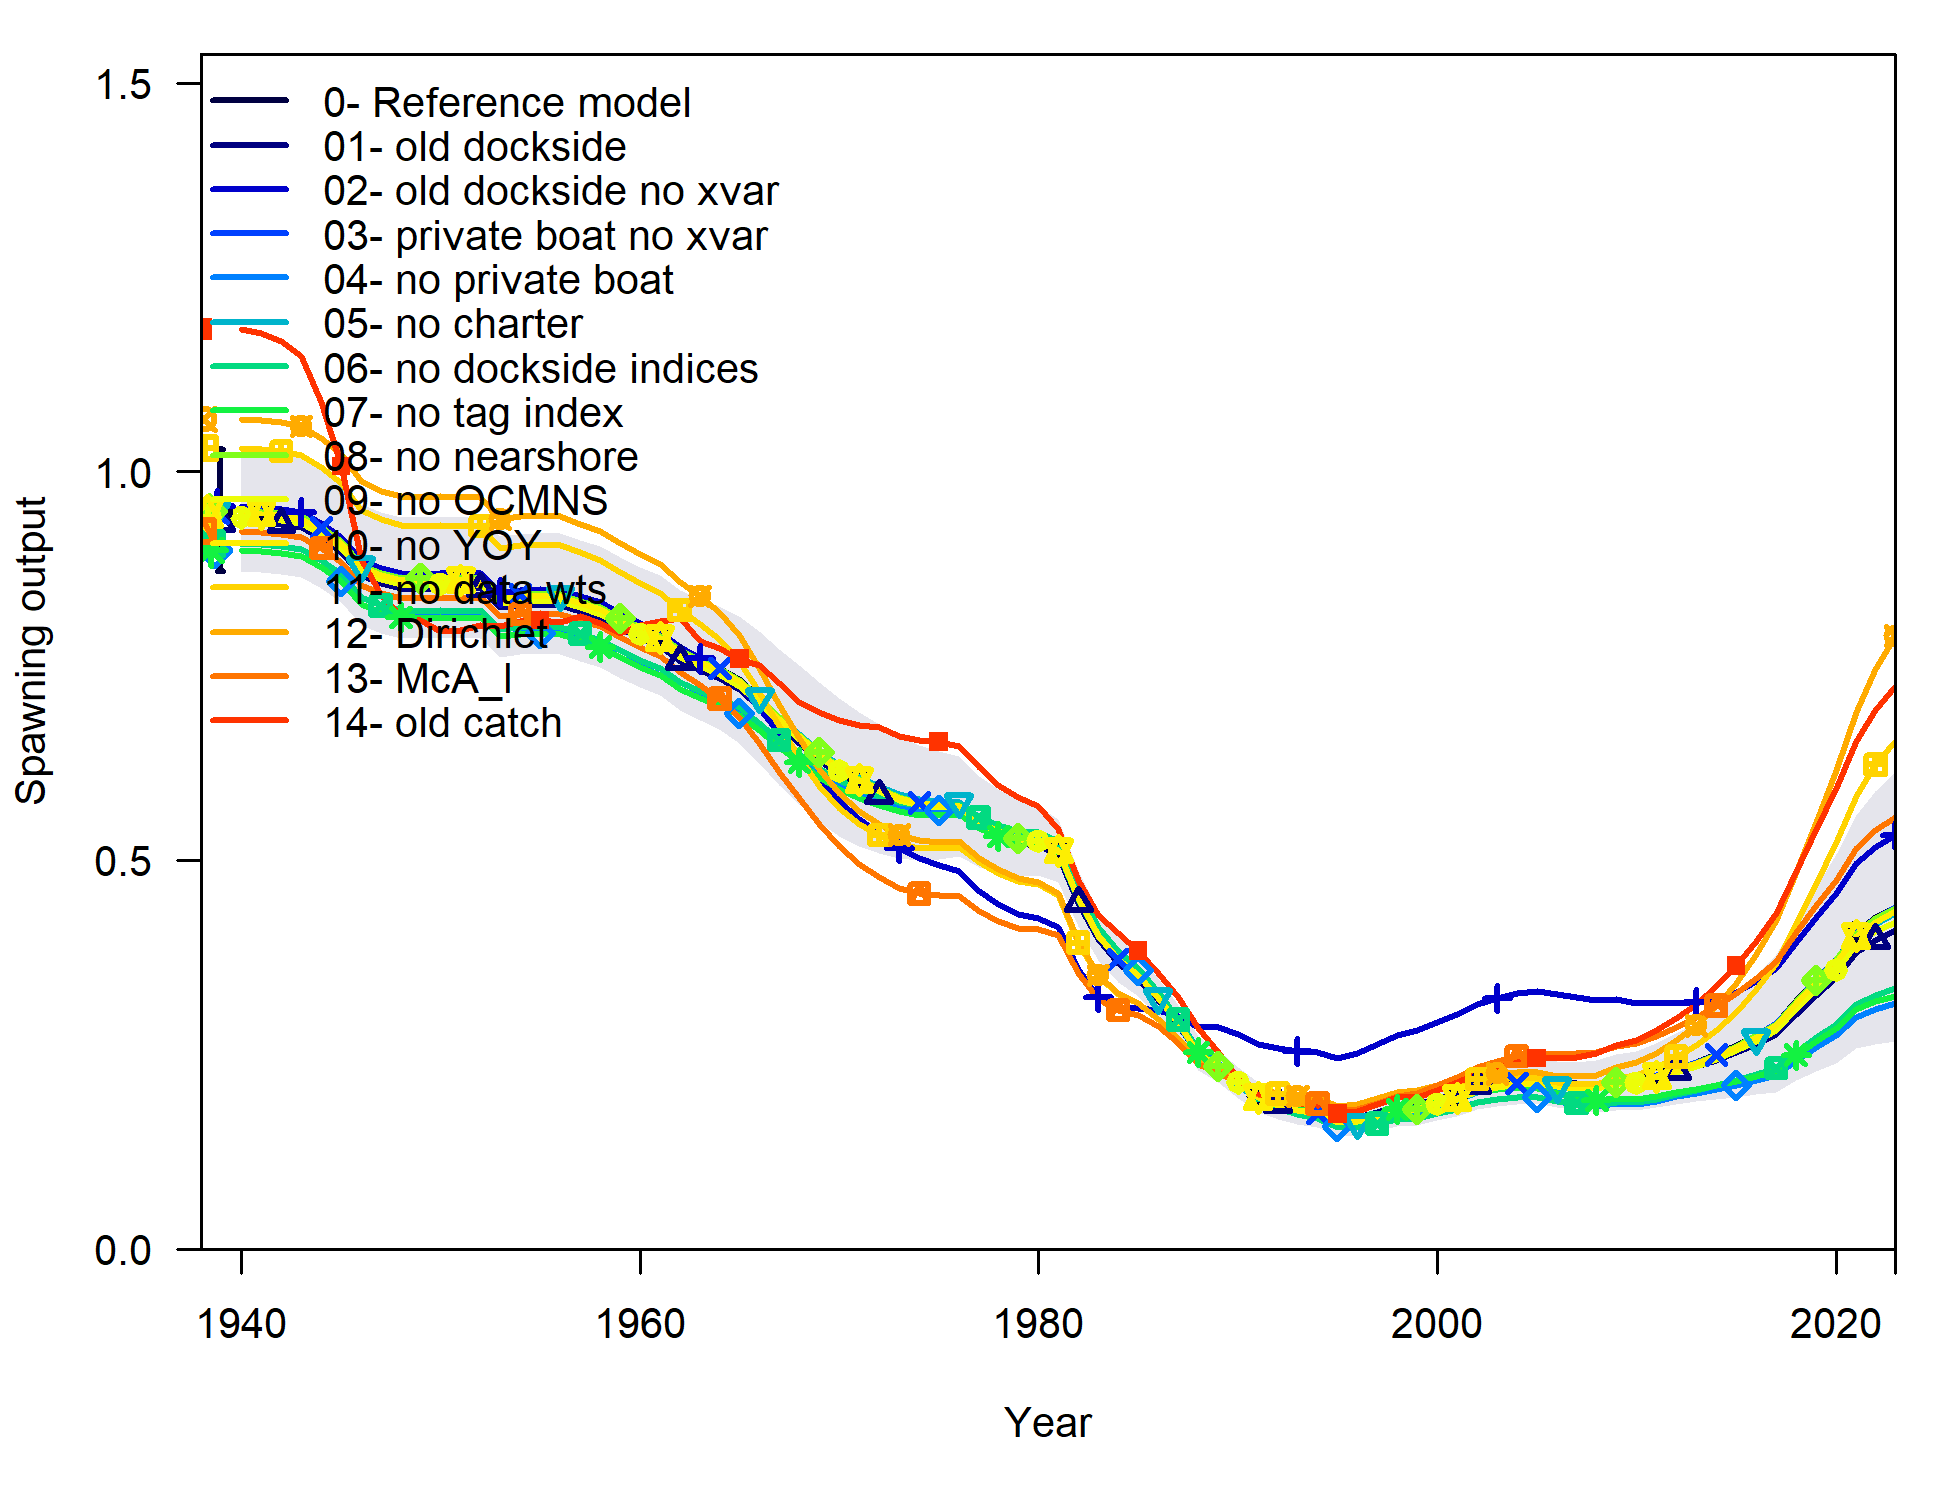
\includegraphics[width=1\textwidth,height=1\textheight]{C:/Users/Jason.Cope/Documents/Github/Sebastes_melanops_WA/Document/figures/modbuild/Mod build stock scale/compare2_spawnbio_uncertainty.png}
\caption{Spawning output (in millions of eggs) time series by data treatment compared to the reference model.\label{fig:modbuild-data-ssb}}
\end{figure}

\hypertarget{jittering}{%
\subsubsection{Jittering}\label{jittering}}

\begin{figure}
\centering
\includegraphics[width=1\textwidth,height=1\textheight]{C:/Users/Jason.Cope/Documents/Github/Sebastes_melanops_WA/Document/figures/modconverge/jitterplot.png}
\caption{Jitter runs (using a value of 0.01) for the Black Rockfish reference model, with jitter run number on the x-axis and -log likelihood value on the y-axis. Blue dot are models that match the likelihood value of the reference model, while red dots deviate from the reference model. All red dots are above the blue dots, indicating no better fit to the reference model was found.\label{fig:jitter}}
\end{figure}

\begin{figure}
\centering
\includegraphics[width=1\textwidth,height=1\textheight]{C:/Users/Jason.Cope/Documents/Github/Sebastes_melanops_WA/Document/figures/modconverge/jitterplot0005.png}
\caption{Jitter runs (using a value of 0.0005) for the Black Rockfish reference model, with jitter run number on the x-axis and -log likelihood value on the y-axis. Blue dot are models that match the likelihood value of the reference model, while red dots deviate from the reference model. All red dots are above the blue dots, indicating no better fit to the reference model was found.\label{fig:jitter0005}}
\end{figure}

\begin{figure}
\centering
\includegraphics[width=1\textwidth,height=1\textheight]{C:/Users/Jason.Cope/Documents/Github/Sebastes_melanops_WA/Document/figures/modconverge/pairs_plot_fast.png}
\caption{Pairs plots of the fastest mixing parameters from running 2000 posterior draws (and keep every draw) using the random walk Metropolis algorithm. Parameters that show little to no movement are recommended to be fixed to improve model speed and efficiency.\label{fig:pairs_plot_fast}}
\end{figure}

\clearpage

\hypertarget{fits-to-data}{%
\subsubsection{Fits to Data}\label{fits-to-data}}

\begin{figure}
\centering
\includegraphics[width=1\textwidth,height=1\textheight]{C:/Users/Jason.Cope/Documents/Github/Sebastes_melanops_WA/Document/models/Reference model/plots/comp_lenfit__multi-fleet_comparison.png}
\caption{Pearson residuals for each fishing fleet and the MPA survey. Closed bubble are positive residuals (observed \textgreater{} expected) and open bubbles are negative residuals (observed \textless{} expected).\label{fig:lt-pearson-resids}}
\end{figure}

\pagebreak

\begin{figure}
\centering
\includegraphics[width=1\textwidth,height=1\textheight]{C:/Users/Jason.Cope/Documents/Github/Sebastes_melanops_WA/Document/models/Reference model/plots/comp_lenfit_data_weighting_TA1.8_Trawl.png}
\caption{Mean length (cm) index from the commercial trawl fishery with 95 percent confidence intervals based on sample sizes and data weighting.\label{fig:trawl-mean-len-fit}}
\end{figure}

\pagebreak

\begin{figure}
\centering
\includegraphics[width=1\textwidth,height=1\textheight]{C:/Users/Jason.Cope/Documents/Github/Sebastes_melanops_WA/Document/models/Reference model/plots/comp_lenfit_data_weighting_TA1.8_NonTRWL.png}
\caption{Mean length (cm) index from the commercial non-trawl fishery with 95 percent confidence intervals based on sample sizes and data weighting.\label{fig:nontrawl-mean-len-fit}}
\end{figure}

\pagebreak

\begin{figure}
\centering
\includegraphics[width=1\textwidth,height=1\textheight]{C:/Users/Jason.Cope/Documents/Github/Sebastes_melanops_WA/Document/models/Reference model/plots/comp_lenfit_data_weighting_TA1.8_Recreational.png}
\caption{Mean length (cm) index from the recreational fishery with 95 percent confidence intervals based on sample sizes and data weighting.\label{fig:rec-mean-len-fit}}
\end{figure}

\pagebreak

\begin{figure}
\centering
\includegraphics[width=1\textwidth,height=1\textheight]{C:/Users/Jason.Cope/Documents/Github/Sebastes_melanops_WA/Document/models/Reference model/plots/comp_lenfit_data_weighting_TA1.8_Tagging.png}
\caption{Mean length (cm) index from tagging survey with 95 percent confidence intervals based on sample sizes and data weighting.\label{fig:tag-mean-len-fit}}
\end{figure}

\pagebreak

\begin{figure}
\centering
\includegraphics[width=1\textwidth,height=1\textheight]{C:/Users/Jason.Cope/Documents/Github/Sebastes_melanops_WA/Document/models/Reference model/plots/comp_lenfit_data_weighting_TA1.8_Nearshore_survey.png}
\caption{Mean length (cm) index from the Nearshore survey with 95 percent confidence intervals based on sample sizes and data weighting.\label{fig:nearshore-mean-len-fit}}
\end{figure}

\pagebreak

\begin{figure}
\centering
\includegraphics[width=1\textwidth,height=1\textheight]{C:/Users/Jason.Cope/Documents/Github/Sebastes_melanops_WA/Document/models/Reference model/plots/comp_lenfit_data_weighting_TA1.8_OCNMS.png}
\caption{Mean length (cm) index from the OCNMS adult dive survey with 95 percent confidence intervals based on sample sizes and data weighting.\label{fig:ocnms-mean-len-fit}}
\end{figure}

\pagebreak

\begin{figure}
\centering
\includegraphics[width=1\textwidth,height=1\textheight]{C:/Users/Jason.Cope/Documents/Github/Sebastes_melanops_WA/Document/models/Reference model/plots/comp_lenfit__aggregated_across_time.png}
\caption{Aggregated length (cm) compositions over all years.\label{fig:agg-len-fit}}
\end{figure}

\pagebreak

\begin{figure}
\centering
\includegraphics[width=1\textwidth,height=1\textheight]{C:/Users/Jason.Cope/Documents/Github/Sebastes_melanops_WA/Document/models/Reference model/plots/comp_condAALfit_data_weighting_TA1.8_condAgeTrawl.png}
\caption{Mean age from conditional age-at-length data for the commercial trawl fishery.\label{fig:trawl-mean-caal}}
\end{figure}

\pagebreak

\begin{figure}
\centering
\includegraphics[width=1\textwidth,height=1\textheight]{C:/Users/Jason.Cope/Documents/Github/Sebastes_melanops_WA/Document/models/Reference model/plots/comp_condAALfit_data_weighting_TA1.8_condAgeNonTRWL.png}
\caption{Mean age observations from the conditional age-at-length data from the commercial non-trawl fishery.\label{fig:nontrawl-mean-caal}}
\end{figure}

\pagebreak

\begin{figure}
\centering
\includegraphics[width=1\textwidth,height=1\textheight]{C:/Users/Jason.Cope/Documents/Github/Sebastes_melanops_WA/Document/models/Reference model/plots/comp_condAALfit_data_weighting_TA1.8_condAgeRecreational.png}
\caption{Mean age observations from the conditional age-at-length data from the recreational fishery.\label{fig:rec-mean-caal}}
\end{figure}

\pagebreak

\begin{figure}
\centering
\includegraphics[width=1\textwidth,height=1\textheight]{C:/Users/Jason.Cope/Documents/Github/Sebastes_melanops_WA/Document/models/Reference model/plots/index2_cpuefit_Charter.png}
\caption{Fit to the charter fishery index of abundance.\label{fig:charter-index-fit}}
\end{figure}

\pagebreak

\begin{figure}
\centering
\includegraphics[width=1\textwidth,height=1\textheight]{C:/Users/Jason.Cope/Documents/Github/Sebastes_melanops_WA/Document/models/Reference model/plots/index2_cpuefit_Private_Boat.png}
\caption{Fit to the private fishery index of abundance.\label{fig:private-index-fit}}
\end{figure}

\pagebreak

\begin{figure}
\centering
\includegraphics[width=1\textwidth,height=1\textheight]{C:/Users/Jason.Cope/Documents/Github/Sebastes_melanops_WA/Document/models/Reference model/plots/index2_cpuefit_Tagging.png}
\caption{Fit to the tagging survey index of abundance.\label{fig:tag-index-fit}}
\end{figure}

\pagebreak

\begin{figure}
\centering
\includegraphics[width=1\textwidth,height=1\textheight]{C:/Users/Jason.Cope/Documents/Github/Sebastes_melanops_WA/Document/models/Reference model/plots/index2_cpuefit_Nearshore_survey.png}
\caption{Fit to the nearshore survey index of abundance.\label{fig:nearshore-index-fit}}
\end{figure}

\pagebreak

\begin{figure}
\centering
\includegraphics[width=1\textwidth,height=1\textheight]{C:/Users/Jason.Cope/Documents/Github/Sebastes_melanops_WA/Document/models/Reference model/plots/index2_cpuefit_OCNMS.png}
\caption{Fit to the OCNMS dive survey index of abundance.\label{fig:ocnms-index-fit}}
\end{figure}

\pagebreak

\begin{figure}
\centering
\includegraphics[width=1\textwidth,height=1\textheight]{C:/Users/Jason.Cope/Documents/Github/Sebastes_melanops_WA/Document/models/Reference model/plots/index2_cpuefit_OCNMS_YOY.png}
\caption{Fit to the OCNMS dive survey index of abundance.\label{fig:ocnms-yoy-index-fit}}
\end{figure}

\pagebreak

\hypertarget{estimated-biology}{%
\subsubsection{Estimated Biology}\label{estimated-biology}}

\hypertarget{recruitment-1}{%
\subsubsection{Recruitment}\label{recruitment-1}}

\begin{figure}
\centering
\includegraphics[width=1\textwidth,height=1\textheight]{C:/Users/Jason.Cope/Documents/Github/Sebastes_melanops_WA/Document/models/Reference model/plots/ts11_Age-0_recruits_(1000s)_with_95_asymptotic_intervals.png}
\caption{Estimated time series of age-0 recruits (1000s).\label{fig:recruits}}
\end{figure}

\pagebreak

\begin{figure}
\centering
\includegraphics[width=1\textwidth,height=1\textheight]{C:/Users/Jason.Cope/Documents/Github/Sebastes_melanops_WA/Document/models/Reference model/plots/recdevs2_withbars.png}
\caption{Estimated time series of recruitment deviations.\label{fig:rec-devs}}
\end{figure}

\pagebreak

\begin{figure}
\centering
\includegraphics[width=1\textwidth,height=1\textheight]{C:/Users/Jason.Cope/Documents/Github/Sebastes_melanops_WA/Document/models/Reference model/plots/recdevs3_varcheck.png}
\caption{Recruitment deviations variance by year. This plot tracks the information content contained in each recruitment deviation. Values below the red line (assumed recruitment variability) indicates years with more informed recruitment deviations.\label{fig:rec-devs-sigmas}}
\end{figure}

\pagebreak

\begin{figure}
\centering
\includegraphics[width=1\textwidth,height=1\textheight]{C:/Users/Jason.Cope/Documents/Github/Sebastes_melanops_WA/Document/models/Reference model/plots/SR_curve.png}
\caption{Stock-recruit curve. Point colors indicate year, with warmer colors indicating earlier years and cooler colors in showing later years.\label{fig:bh-curve}}
\end{figure}

\pagebreak

\begin{figure}
\centering
\includegraphics[width=1\textwidth,height=1\textheight]{C:/Users/Jason.Cope/Documents/Github/Sebastes_melanops_WA/Document/models/Reference model/plots/recruit_fit_bias_adjust.png}
\caption{Recruitment bias adjustment applied in the reference model.\label{fig:bias-adj}}
\end{figure}

\begin{figure}
\centering
\includegraphics[width=1\textwidth,height=1\textheight]{C:/Users/Jason.Cope/Documents/Github/Sebastes_melanops_WA/Document/models/Reference model/plots/recdevs3_varcheck.png}
\caption{Recruitment deviations variance check. Low standard deviations indicate years with informative deviations .\label{fig:varcheck}}
\end{figure}

\pagebreak

\hypertarget{selectivity}{%
\subsubsection{Selectivity}\label{selectivity}}

\begin{figure}
\centering
\includegraphics[width=1\textwidth,height=1\textheight]{C:/Users/Jason.Cope/Documents/Github/Sebastes_melanops_WA/Document/models/Reference model/plots/sel01_multiple_fleets_length1.png}
\caption{Length-based selectivity curves for each fleet and survey.\label{fig:fleet_selectivity}}
\end{figure}

\pagebreak

\hypertarget{time-series}{%
\subsubsection{Time series}\label{time-series}}

\begin{figure}
\centering
\includegraphics[width=1\textwidth,height=1\textheight]{C:/Users/Jason.Cope/Documents/Github/Sebastes_melanops_WA/Document/models/Reference model/plots/ts7_Spawning_output_with_95_asymptotic_intervals_intervals.png}
\caption{Estimated time series of spawning output (in millions of eggs).\label{fig:ssb}}
\end{figure}

\pagebreak

\begin{figure}
\centering
\includegraphics[width=1\textwidth,height=1\textheight]{C:/Users/Jason.Cope/Documents/Github/Sebastes_melanops_WA/Document/models/Reference model/plots/ts1_Total_biomass_(mt).png}
\caption{Estimated time series of total biomass (mt).\label{fig:tot-bio}}
\end{figure}

\pagebreak

\begin{figure}
\centering
\includegraphics[width=1\textwidth,height=1\textheight]{C:/Users/Jason.Cope/Documents/Github/Sebastes_melanops_WA/Document/models/Reference model/plots/ts9_Relative_spawning_output_intervals.png}
\caption{Estimated time series of fraction of unfished spawning output.\label{fig:depl}}
\end{figure}

\pagebreak

\begin{figure}
\centering
\includegraphics[width=1\textwidth,height=1\textheight]{C:/Users/Jason.Cope/Documents/Github/Sebastes_melanops_WA/Document/figures/comp_2015_2023/compare2_spawnbio_uncertainty.png}
\caption{Comparison of the time series of spawning output between the 2015 and 2023 assessment results.\label{fig:comp_ssb}}
\end{figure}

\pagebreak

\begin{figure}
\centering
\includegraphics[width=1\textwidth,height=1\textheight]{C:/Users/Jason.Cope/Documents/Github/Sebastes_melanops_WA/Document/figures/comp_2015_2023/compare4_Bratio_uncertainty.png}
\caption{Comparison of the time series of relative spawning output between the 2015 and 2023 assessment results.\label{fig:comp_depl}}
\end{figure}

\pagebreak

\hypertarget{sensitivities}{%
\subsubsection{Sensitivities}\label{sensitivities}}

\begin{figure}
\centering
\includegraphics[width=1\textwidth,height=1\textheight]{C:/Users/Jason.Cope/Documents/Github/Sebastes_melanops_WA/Document/figures/sensi_data/Sensi_logREplot_SB_Dep_F_MSY.png}
\caption{Log relative change (log((Model\_sensi-Model\_ref)/Model\_ref)) in data treatment for 5 derived quantities. Colored boxes indicate 95 percent confidence interval of the reference model.\label{fig:sensi-data-RE}}
\end{figure}

\pagebreak

\begin{figure}
\centering
\includegraphics[width=1\textwidth,height=1\textheight]{C:/Users/Jason.Cope/Documents/Github/Sebastes_melanops_WA/Document/figures/sensi_data/compare2_spawnbio_uncertainty.png}
\caption{Spawning output (in millions of eggs) time series by data treatment compared to the reference model.\label{fig:sensi-data-ssb}}
\end{figure}

\pagebreak

\begin{figure}
\centering
\includegraphics[width=1\textwidth,height=1\textheight]{C:/Users/Jason.Cope/Documents/Github/Sebastes_melanops_WA/Document/figures/sensi_data/compare4_Bratio_uncertainty.png}
\caption{Relative spawning output time series by data treatment compared to the reference model. Missing scenarios mean the spawning output was too large to show.\label{fig:sensi-data-depl}}
\end{figure}

\pagebreak

\begin{figure}
\centering
\includegraphics[width=1\textwidth,height=1\textheight]{C:/Users/Jason.Cope/Documents/Github/Sebastes_melanops_WA/Document/figures/sensi_modspex/Sensi_logREplot_SB_Dep_F_MSY.png}
\caption{Log relative change (log((Model\_sensi-Model\_ref)/Model\_ref)) in model specification scenario for 5 derived quantities. Colored boxes indicate 95 percent confidence interval of the reference model.\label{fig:sensi-modspec-RE}}
\end{figure}

\pagebreak

\begin{figure}
\centering
\includegraphics[width=1\textwidth,height=1\textheight]{C:/Users/Jason.Cope/Documents/Github/Sebastes_melanops_WA/Document/figures/sensi_modspex/compare2_spawnbio_uncertainty.png}
\caption{Spawning output (in millions of eggs) time series by model specification scenario compared to the reference model. Missing scenarios mean the spawning output was too large to show.\label{fig:sensi-modspec-ssb}}
\end{figure}

\pagebreak

\begin{figure}
\centering
\includegraphics[width=1\textwidth,height=1\textheight]{C:/Users/Jason.Cope/Documents/Github/Sebastes_melanops_WA/Document/figures/sensi_modspex/compare4_Bratio_uncertainty.png}
\caption{Relative spawning output time series by model specification scenario compared to the reference model.\label{fig:sensi-modspec-depl}}
\end{figure}

\pagebreak

\hypertarget{likelihood-profiles-1}{%
\subsubsection{Likelihood Profiles}\label{likelihood-profiles-1}}

\begin{figure}
\centering
\includegraphics[width=1\textwidth,height=1\textheight]{C:/Users/Jason.Cope/Documents/Github/Sebastes_melanops_WA/Document/figures/likelihoods/parameter_panel_SR_LN(R0).png}
\caption{Initial recruitment (\(lnR_0\)) likelihood profile (change in the negative log-likelihood across a range of \(ln(R0)\) values) and derived quantities. Red line in the top left figure indicates the significance level in likelihood difference.\label{fig:R0-profile}}
\end{figure}

\pagebreak

\begin{figure}
\centering
\includegraphics[width=1\textwidth,height=1\textheight]{C:/Users/Jason.Cope/Documents/Github/Sebastes_melanops_WA/Document/figures/likelihoods/piner_panel_SR_LN(R0).png}
\caption{Initial recruitment (\(ln(R0)\)) likelihood profile for each of the likelihood components.\label{fig:R0-profile-components}}
\end{figure}

\pagebreak

\begin{figure}
\centering
\includegraphics[width=1\textwidth,height=1\textheight]{C:/Users/Jason.Cope/Documents/Github/Sebastes_melanops_WA/Document/figures/likelihoods/parameter_panel_SR_BH_steep.png}
\caption{Beverton-Holt steepness parameter likelihood profile (change in the negative log-likelihood across a range of steepness values) and derived quantities. Red line in the top left figure indicates the significance level in likelihood difference.\label{fig:steepness-profile}}
\end{figure}

\pagebreak

\begin{figure}
\centering
\includegraphics[width=1\textwidth,height=1\textheight]{C:/Users/Jason.Cope/Documents/Github/Sebastes_melanops_WA/Document/figures/likelihoods/piner_panel_SR_BH_steep.png}
\caption{Beverton-Holt steepness parameter likelihood profile for each of the likelihood components.\label{fig:steepness-profile-components}}
\end{figure}

\pagebreak

\begin{figure}
\centering
\includegraphics[width=1\textwidth,height=1\textheight]{C:/Users/Jason.Cope/Documents/Github/Sebastes_melanops_WA/Document/figures/likelihoods/M_fm_multilikelihood_profile.png}
\caption{Female and male \(M\) multi-parameter likelihood profile and derived quantities. Red lines in the top left figure indicate significantly similar values compared to the reference model. Broken and solid lines in the bottom right figure indicate target and limit referene points, respectively.\label{fig:M-multiprofile-combo}}
\end{figure}

\pagebreak

\hypertarget{retrospectives}{%
\subsubsection{Retrospectives}\label{retrospectives}}

\begin{figure}
\centering
\includegraphics[width=1\textwidth,height=1\textheight]{C:/Users/Jason.Cope/Documents/Github/Sebastes_melanops_WA/Document/figures/retro/compare2_spawnbio_uncertainty.png}
\caption{Change in the estimate of spawning output when the most recent 10 years of data area removed sequentially.\label{fig:retro-ssb}}
\end{figure}

\pagebreak

\begin{figure}
\centering
\includegraphics[width=1\textwidth,height=1\textheight]{C:/Users/Jason.Cope/Documents/Github/Sebastes_melanops_WA/Document/figures/retro/compare4_Bratio_uncertainty.png}
\caption{Change in the estimate of fraction unfished when the most recent 10 years of data area removed sequentially.\label{fig:retro-depl}}
\end{figure}

\newpage

\begin{figure}
\centering
\includegraphics[width=1\textwidth,height=1\textheight]{C:/Users/Jason.Cope/Documents/Github/Sebastes_melanops_WA/Document/models/Reference model/plots/SPR4_phase.png}
\caption{Phase plot of biomass ratio vs.~SPR ratio. Each point represents the biomass ratio at the start of the year and the relative fishing intensity in that same year. Warmer colors (red) represent early years and colder colors (blue) represent recent years.\label{fig:phase}}
\end{figure}

\pagebreak

\begin{figure}
\centering
\includegraphics[width=1\textwidth,height=1\textheight]{C:/Users/Jason.Cope/Documents/Github/Sebastes_melanops_WA/Document/models/Reference model/plots/SPR2_minusSPRseries.png}
\caption{Estimated time series of fishing intensity, 1-SPR.\label{fig:1-spr}}
\end{figure}

\pagebreak

\begin{figure}
\centering
\includegraphics[width=1\textwidth,height=1\textheight]{C:/Users/Jason.Cope/Documents/Github/Sebastes_melanops_WA/Document/models/Reference model/plots/yield2_yield_curve_with_refpoints.png}
\caption{Equilibrium yield curve for the base case model. Values are based on (the time invariant) fishery selectivities and with steepness fixed at 0.72.\label{fig:yield}}
\end{figure}

\pagebreak

\clearpage

\hypertarget{app-a}{%
\section{Appendix A: Detailed Fit to Length Composition Data}\label{app-a}}

\begin{figure}
\centering
\includegraphics[width=1\textwidth,height=1\textheight]{C:/Users/Jason.Cope/Documents/Github/Sebastes_melanops_WA/Document/models/Reference model/plots/comp_lenfit_flt1mkt0_page1.png}
\caption{Length comps, whole catch, Trawl (plot 1 of 2).`N adj.' is the input sample size after data-weighting adjustment. N eff. is the calculated effective sample size used in the McAllister-Ianelli tuning method.\label{fig:comp_lenfit_flt1mkt0_page1}}
\end{figure}

\begin{figure}
\centering
\includegraphics[width=1\textwidth,height=1\textheight]{C:/Users/Jason.Cope/Documents/Github/Sebastes_melanops_WA/Document/models/Reference model/plots/comp_lenfit_flt1mkt0_page2.png}
\caption{Length comps, whole catch, Trawl (plot 1 of 2).`N adj.' is the input sample size after data-weighting adjustment. N eff. is the calculated effective sample size used in the McAllister-Ianelli tuning method. (plot 2 of 2).\label{fig:comp_lenfit_flt1mkt0_page2}}
\end{figure}

\begin{figure}
\centering
\includegraphics[width=1\textwidth,height=1\textheight]{C:/Users/Jason.Cope/Documents/Github/Sebastes_melanops_WA/Document/models/Reference model/plots/comp_lenfit_flt2mkt0.png}
\caption{Length comps, whole catch, NonTRWL.`N adj.' is the input sample size after data-weighting adjustment. N eff. is the calculated effective sample size used in the McAllister-Ianelli tuning method.\label{fig:comp_lenfit_flt2mkt0}}
\end{figure}

\begin{figure}
\centering
\includegraphics[width=1\textwidth,height=1\textheight]{C:/Users/Jason.Cope/Documents/Github/Sebastes_melanops_WA/Document/models/Reference model/plots/comp_lenfit_flt3mkt0_page1.png}
\caption{Length comps, whole catch, Recreational (plot 1 of 2).`N adj.' is the input sample size after data-weighting adjustment. N eff. is the calculated effective sample size used in the McAllister-Ianelli tuning method.\label{fig:comp_lenfit_flt3mkt0_page1}}
\end{figure}

\begin{figure}
\centering
\includegraphics[width=1\textwidth,height=1\textheight]{C:/Users/Jason.Cope/Documents/Github/Sebastes_melanops_WA/Document/models/Reference model/plots/comp_lenfit_flt3mkt0_page2.png}
\caption{Length comps, whole catch, Recreational (plot 1 of 2).`N adj.' is the input sample size after data-weighting adjustment. N eff. is the calculated effective sample size used in the McAllister-Ianelli tuning method. (plot 2 of 2).\label{fig:comp_lenfit_flt3mkt0_page2}}
\end{figure}

\begin{figure}
\centering
\includegraphics[width=1\textwidth,height=1\textheight]{C:/Users/Jason.Cope/Documents/Github/Sebastes_melanops_WA/Document/models/Reference model/plots/comp_lenfit_flt4mkt0.png}
\caption{Length comps, whole catch, Tagging.`N adj.' is the input sample size after data-weighting adjustment. N eff. is the calculated effective sample size used in the McAllister-Ianelli tuning method.\label{fig:comp_lenfit_flt4mkt0}}
\end{figure}

\begin{figure}
\centering
\includegraphics[width=1\textwidth,height=1\textheight]{C:/Users/Jason.Cope/Documents/Github/Sebastes_melanops_WA/Document/models/Reference model/plots/comp_lenfit_flt5mkt0.png}
\caption{Length comps, whole catch, Nearshore\_survey.`N adj.' is the input sample size after data-weighting adjustment. N eff. is the calculated effective sample size used in the McAllister-Ianelli tuning method.\label{fig:comp_lenfit_flt5mkt0}}
\end{figure}

\begin{figure}
\centering
\includegraphics[width=1\textwidth,height=1\textheight]{C:/Users/Jason.Cope/Documents/Github/Sebastes_melanops_WA/Document/models/Reference model/plots/comp_lenfit_flt6mkt0.png}
\caption{Length comps, whole catch, OCNMS.`N adj.' is the input sample size after data-weighting adjustment. N eff. is the calculated effective sample size used in the McAllister-Ianelli tuning method.\label{fig:comp_lenfit_flt6mkt0}}
\end{figure}

\clearpage

\hypertarget{app-b}{%
\section{Appendix B: Fit to Conditional-Age-at-Length Composition Data}\label{app-b}}

\begin{figure}
\centering
\includegraphics[width=1\textwidth,height=1\textheight]{C:/Users/Jason.Cope/Documents/Github/Sebastes_melanops_WA/Document/models/Reference model/plots/comp_condAALfit_residsflt1mkt0_page1.png}
\caption{Pearson residuals, whole catch, Trawl (max=8.72) (plot 1 of 3).\label{fig:comp_condAALfit_residsflt1mkt0_page1}}
\end{figure}

\begin{figure}
\centering
\includegraphics[width=1\textwidth,height=1\textheight]{C:/Users/Jason.Cope/Documents/Github/Sebastes_melanops_WA/Document/models/Reference model/plots/comp_condAALfit_residsflt1mkt0_page2.png}
\caption{Pearson residuals, whole catch, Trawl (max=8.72) (plot 2 of 3).\label{fig:comp_condAALfit_residsflt1mkt0_page2}}
\end{figure}

\begin{figure}
\centering
\includegraphics[width=1\textwidth,height=1\textheight]{C:/Users/Jason.Cope/Documents/Github/Sebastes_melanops_WA/Document/models/Reference model/plots/comp_condAALfit_residsflt1mkt0_page3.png}
\caption{Pearson residuals, whole catch, Trawl (max=8.72) (plot 3 of 3).\label{fig:comp_condAALfit_residsflt1mkt0_page3}}
\end{figure}

\begin{figure}
\centering
\includegraphics[width=1\textwidth,height=1\textheight]{C:/Users/Jason.Cope/Documents/Github/Sebastes_melanops_WA/Document/models/Reference model/plots/comp_condAALfit_residsflt2mkt0_page1.png}
\caption{Pearson residuals, whole catch, NonTRWL (max=18.53) (plot 1 of 3).\label{fig:comp_condAALfit_residsflt2mkt0_page1}}
\end{figure}

\begin{figure}
\centering
\includegraphics[width=1\textwidth,height=1\textheight]{C:/Users/Jason.Cope/Documents/Github/Sebastes_melanops_WA/Document/models/Reference model/plots/comp_condAALfit_residsflt2mkt0_page2.png}
\caption{Pearson residuals, whole catch, NonTRWL (max=18.53) (plot 2 of 3).\label{fig:comp_condAALfit_residsflt2mkt0_page2}}
\end{figure}

\begin{figure}
\centering
\includegraphics[width=1\textwidth,height=1\textheight]{C:/Users/Jason.Cope/Documents/Github/Sebastes_melanops_WA/Document/models/Reference model/plots/comp_condAALfit_residsflt2mkt0_page3.png}
\caption{Pearson residuals, whole catch, NonTRWL (max=18.53) (plot 3 of 3).\label{fig:comp_condAALfit_residsflt2mkt0_page3}}
\end{figure}

\begin{figure}
\centering
\includegraphics[width=1\textwidth,height=1\textheight]{C:/Users/Jason.Cope/Documents/Github/Sebastes_melanops_WA/Document/models/Reference model/plots/comp_condAALfit_residsflt3mkt0_page1.png}
\caption{Pearson residuals, whole catch, Recreational (max=25.87) (plot 1 of 8).\label{fig:comp_condAALfit_residsflt3mkt0_page1}}
\end{figure}

\begin{figure}
\centering
\includegraphics[width=1\textwidth,height=1\textheight]{C:/Users/Jason.Cope/Documents/Github/Sebastes_melanops_WA/Document/models/Reference model/plots/comp_condAALfit_residsflt3mkt0_page2.png}
\caption{Pearson residuals, whole catch, Recreational (max=25.87) (plot 2 of 8).\label{fig:comp_condAALfit_residsflt3mkt0_page2}}
\end{figure}

\begin{figure}
\centering
\includegraphics[width=1\textwidth,height=1\textheight]{C:/Users/Jason.Cope/Documents/Github/Sebastes_melanops_WA/Document/models/Reference model/plots/comp_condAALfit_residsflt3mkt0_page3.png}
\caption{Pearson residuals, whole catch, Recreational (max=25.87) (plot 3 of 8).\label{fig:comp_condAALfit_residsflt3mkt0_page3}}
\end{figure}

\begin{figure}
\centering
\includegraphics[width=1\textwidth,height=1\textheight]{C:/Users/Jason.Cope/Documents/Github/Sebastes_melanops_WA/Document/models/Reference model/plots/comp_condAALfit_residsflt3mkt0_page4.png}
\caption{Pearson residuals, whole catch, Recreational (max=25.87) (plot 4 of 8).\label{fig:comp_condAALfit_residsflt3mkt0_page4}}
\end{figure}

\begin{figure}
\centering
\includegraphics[width=1\textwidth,height=1\textheight]{C:/Users/Jason.Cope/Documents/Github/Sebastes_melanops_WA/Document/models/Reference model/plots/comp_condAALfit_residsflt3mkt0_page5.png}
\caption{Pearson residuals, whole catch, Recreational (max=25.87) (plot 5 of 8).\label{fig:comp_condAALfit_residsflt3mkt0_page5}}
\end{figure}

\begin{figure}
\centering
\includegraphics[width=1\textwidth,height=1\textheight]{C:/Users/Jason.Cope/Documents/Github/Sebastes_melanops_WA/Document/models/Reference model/plots/comp_condAALfit_residsflt3mkt0_page6.png}
\caption{Pearson residuals, whole catch, Recreational (max=25.87) (plot 6 of 8).\label{fig:comp_condAALfit_residsflt3mkt0_page6}}
\end{figure}

\begin{figure}
\centering
\includegraphics[width=1\textwidth,height=1\textheight]{C:/Users/Jason.Cope/Documents/Github/Sebastes_melanops_WA/Document/models/Reference model/plots/comp_condAALfit_residsflt3mkt0_page7.png}
\caption{Pearson residuals, whole catch, Recreational (max=25.87) (plot 7 of 8).\label{fig:comp_condAALfit_residsflt3mkt0_page7}}
\end{figure}

\begin{figure}
\centering
\includegraphics[width=1\textwidth,height=1\textheight]{C:/Users/Jason.Cope/Documents/Github/Sebastes_melanops_WA/Document/models/Reference model/plots/comp_condAALfit_residsflt3mkt0_page8.png}
\caption{Pearson residuals, whole catch, Recreational (max=25.87) (plot 8 of 8).\label{fig:comp_condAALfit_residsflt3mkt0_page8}}
\end{figure}

\clearpage

\hypertarget{app-c}{%
\section{Appendix C: Fit to Conditional-Age-at-Length Composition Data}\label{app-c}}

\begin{figure}
\centering
\includegraphics[width=1\textwidth,height=1\textheight]{C:/Users/Jason.Cope/Documents/Github/Sebastes_melanops_WA/Document/models/Reference model/plots/comp_condAALfit_Andre_plotsflt1mkt0_page1.png}
\caption{Trawl fishery conditional AAL plot (plot 1 of 5) showing mean age (left panel) and standard deviation (right panel. Shaded areas are 90 percent CIs).\label{fig:comp_condAALfit_Andre_plotsflt1mkt0_page1}}
\end{figure}

\begin{figure}
\centering
\includegraphics[width=1\textwidth,height=1\textheight]{C:/Users/Jason.Cope/Documents/Github/Sebastes_melanops_WA/Document/models/Reference model/plots/comp_condAALfit_Andre_plotsflt1mkt0_page2.png}
\caption{Trawl conditional AAL plot (plot 2 of 5).\label{fig:comp_condAALfit_Andre_plotsflt1mkt0_page2}}
\end{figure}

\begin{figure}
\centering
\includegraphics[width=1\textwidth,height=1\textheight]{C:/Users/Jason.Cope/Documents/Github/Sebastes_melanops_WA/Document/models/Reference model/plots/comp_condAALfit_Andre_plotsflt1mkt0_page3.png}
\caption{Trawl conditional AAL plot (plot 3 of 5).\label{fig:comp_condAALfit_Andre_plotsflt1mkt0_page3}}
\end{figure}

\begin{figure}
\centering
\includegraphics[width=1\textwidth,height=1\textheight]{C:/Users/Jason.Cope/Documents/Github/Sebastes_melanops_WA/Document/models/Reference model/plots/comp_condAALfit_Andre_plotsflt1mkt0_page4.png}
\caption{Trawl conditional AAL plot (plot 4 of 5).\label{fig:comp_condAALfit_Andre_plotsflt1mkt0_page4}}
\end{figure}

\begin{figure}
\centering
\includegraphics[width=1\textwidth,height=1\textheight]{C:/Users/Jason.Cope/Documents/Github/Sebastes_melanops_WA/Document/models/Reference model/plots/comp_condAALfit_Andre_plotsflt1mkt0_page5.png}
\caption{Trawl conditional AAL plot (plot 5 of 5).\label{fig:comp_condAALfit_Andre_plotsflt1mkt0_page5}}
\end{figure}

\begin{figure}
\centering
\includegraphics[width=1\textwidth,height=1\textheight]{C:/Users/Jason.Cope/Documents/Github/Sebastes_melanops_WA/Document/models/Reference model/plots/comp_condAALfit_Andre_plotsflt2mkt0_page1.png}
\caption{Non-trawl (jig) fishery conditional AAL plot (plot 1 of 2) showing mean age (left panel) and standard deviation (right panel. Shaded areas are 90 percent CIs).\label{fig:comp_condAALfit_Andre_plotsflt2mkt0_page1}}
\end{figure}

\begin{figure}
\centering
\includegraphics[width=1\textwidth,height=1\textheight]{C:/Users/Jason.Cope/Documents/Github/Sebastes_melanops_WA/Document/models/Reference model/plots/comp_condAALfit_Andre_plotsflt2mkt0_page2.png}
\caption{Non-trawl (jig) conditional AAL plot (plot 2 of 2).\label{fig:comp_condAALfit_Andre_plotsflt2mkt0_page2}}
\end{figure}

\begin{figure}
\centering
\includegraphics[width=1\textwidth,height=1\textheight]{C:/Users/Jason.Cope/Documents/Github/Sebastes_melanops_WA/Document/models/Reference model/plots/comp_condAALfit_Andre_plotsflt2mkt0_page3.png}
\caption{Non-trawl (jig) conditional AAL plot (plot 3 of 3).\label{fig:comp_condAALfit_Andre_plotsflt2mkt0_page3}}
\end{figure}

\begin{figure}
\centering
\includegraphics[width=1\textwidth,height=1\textheight]{C:/Users/Jason.Cope/Documents/Github/Sebastes_melanops_WA/Document/models/Reference model/plots/comp_condAALfit_Andre_plotsflt3mkt0_page1.png}
\caption{Ocean boat conditional AAL plot (plot 1 of 11) showing mean age (left panel) and standard deviation (right panel. Shaded areas are 90 percent CIs).\label{fig:comp_condAALfit_Andre_plotsflt3mkt0_page1}}
\end{figure}

\begin{figure}
\centering
\includegraphics[width=1\textwidth,height=1\textheight]{C:/Users/Jason.Cope/Documents/Github/Sebastes_melanops_WA/Document/models/Reference model/plots/comp_condAALfit_Andre_plotsflt3mkt0_page10.png}
\caption{Ocean boat conditional AAL plot (plot 2 of 11).\label{fig:comp_condAALfit_Andre_plotsflt3mkt0_page10}}
\end{figure}

\begin{figure}
\centering
\includegraphics[width=1\textwidth,height=1\textheight]{C:/Users/Jason.Cope/Documents/Github/Sebastes_melanops_WA/Document/models/Reference model/plots/comp_condAALfit_Andre_plotsflt3mkt0_page11.png}
\caption{Ocean boat conditional AAL plot (plot 3 of 11).\label{fig:comp_condAALfit_Andre_plotsflt3mkt0_page11}}
\end{figure}

\begin{figure}
\centering
\includegraphics[width=1\textwidth,height=1\textheight]{C:/Users/Jason.Cope/Documents/Github/Sebastes_melanops_WA/Document/models/Reference model/plots/comp_condAALfit_Andre_plotsflt3mkt0_page2.png}
\caption{Ocean boat conditional AAL plot (plot 3 of 11).\label{fig:comp_condAALfit_Andre_plotsflt3mkt0_page2}}
\end{figure}

\begin{figure}
\centering
\includegraphics[width=1\textwidth,height=1\textheight]{C:/Users/Jason.Cope/Documents/Github/Sebastes_melanops_WA/Document/models/Reference model/plots/comp_condAALfit_Andre_plotsflt3mkt0_page3.png}
\caption{Ocean boat conditional AAL plot (plot 4 of 11).\label{fig:comp_condAALfit_Andre_plotsflt3mkt0_page3}}
\end{figure}

\begin{figure}
\centering
\includegraphics[width=1\textwidth,height=1\textheight]{C:/Users/Jason.Cope/Documents/Github/Sebastes_melanops_WA/Document/models/Reference model/plots/comp_condAALfit_Andre_plotsflt3mkt0_page4.png}
\caption{Ocean boat conditional AAL plot (plot 5 of 11).\label{fig:comp_condAALfit_Andre_plotsflt3mkt0_page4}}
\end{figure}

\begin{figure}
\centering
\includegraphics[width=1\textwidth,height=1\textheight]{C:/Users/Jason.Cope/Documents/Github/Sebastes_melanops_WA/Document/models/Reference model/plots/comp_condAALfit_Andre_plotsflt3mkt0_page5.png}
\caption{Ocean boat conditional AAL plot (plot 6 of 11).\label{fig:comp_condAALfit_Andre_plotsflt3mkt0_page5}}
\end{figure}

\begin{figure}
\centering
\includegraphics[width=1\textwidth,height=1\textheight]{C:/Users/Jason.Cope/Documents/Github/Sebastes_melanops_WA/Document/models/Reference model/plots/comp_condAALfit_Andre_plotsflt3mkt0_page6.png}
\caption{Ocean boat conditional AAL plot (plot 7 of 11).\label{fig:comp_condAALfit_Andre_plotsflt3mkt0_page6}}
\end{figure}

\begin{figure}
\centering
\includegraphics[width=1\textwidth,height=1\textheight]{C:/Users/Jason.Cope/Documents/Github/Sebastes_melanops_WA/Document/models/Reference model/plots/comp_condAALfit_Andre_plotsflt3mkt0_page7.png}
\caption{Ocean boat conditional AAL plot (plot 8 of 11).\label{fig:comp_condAALfit_Andre_plotsflt3mkt0_page7}}
\end{figure}

\begin{figure}
\centering
\includegraphics[width=1\textwidth,height=1\textheight]{C:/Users/Jason.Cope/Documents/Github/Sebastes_melanops_WA/Document/models/Reference model/plots/comp_condAALfit_Andre_plotsflt3mkt0_page8.png}
\caption{Ocean boat conditional AAL plot (plot 9 of 11).\label{fig:comp_condAALfit_Andre_plotsflt3mkt0_page8}}
\end{figure}

\begin{figure}
\centering
\includegraphics[width=1\textwidth,height=1\textheight]{C:/Users/Jason.Cope/Documents/Github/Sebastes_melanops_WA/Document/models/Reference model/plots/comp_condAALfit_Andre_plotsflt3mkt0_page9.png}
\caption{Ocean boat conditional AAL plot (plot 10 of 11).\label{fig:comp_condAALfit_Andre_plotsflt3mkt0_page9}}
\end{figure}

\clearpage

\hypertarget{app-d}{%
\section{Appendix D: Passive Fit to Marginal Age Composition Data}\label{app-d}}

\begin{figure}
\centering
\includegraphics[width=1\textwidth,height=1\textheight]{C:/Users/Jason.Cope/Documents/Github/Sebastes_melanops_WA/Document/models/Reference model/plots/comp_gstagefit_flt1mkt0.png}
\caption{Excluded age comps, whole catch, Trawl.`N adj.' is the input sample size after data-weighting adjustment. N eff. is the calculated effective sample size used in the McAllister-Ianelli tuning method.\label{fig:comp_gstagefit_flt1mkt0}}
\end{figure}

\begin{figure}
\centering
\includegraphics[width=1\textwidth,height=1\textheight]{C:/Users/Jason.Cope/Documents/Github/Sebastes_melanops_WA/Document/models/Reference model/plots/comp_gstagefit_flt2mkt0.png}
\caption{Excluded age comps, whole catch, NonTRWL.`N adj.' is the input sample size after data-weighting adjustment. N eff. is the calculated effective sample size used in the McAllister-Ianelli tuning method.\label{fig:comp_gstagefit_flt2mkt0}}
\end{figure}

\begin{figure}
\centering
\includegraphics[width=1\textwidth,height=1\textheight]{C:/Users/Jason.Cope/Documents/Github/Sebastes_melanops_WA/Document/models/Reference model/plots/comp_gstagefit_flt3mkt0_page1.png}
\caption{Excluded age comps, whole catch, Recreational (plot 1 of 2).`N adj.' is the input sample size after data-weighting adjustment. N eff. is the calculated effective sample size used in the McAllister-Ianelli tuning method.\label{fig:comp_gstagefit_flt3mkt0_page1}}
\end{figure}

\begin{figure}
\centering
\includegraphics[width=1\textwidth,height=1\textheight]{C:/Users/Jason.Cope/Documents/Github/Sebastes_melanops_WA/Document/models/Reference model/plots/comp_gstagefit_flt3mkt0_page2.png}
\caption{Excluded age comps, whole catch, Recreational (plot 1 of 2).`N adj.' is the input sample size after data-weighting adjustment. N eff. is the calculated effective sample size used in the McAllister-Ianelli tuning method. (plot 2 of 2).\label{fig:comp_gstagefit_flt3mkt0_page2}}
\end{figure}

\clearpage

\hypertarget{app-e}{%
\section{Appendix E: Numbers at Age Plot}\label{app-e}}

\hypertarget{females}{%
\subsection{Females}\label{females}}

\begin{figure}
\centering
\includegraphics[width=1\textwidth,height=1\textheight]{C:/Users/Jason.Cope/Documents/Github/Sebastes_melanops_WA/Document/models/Reference model/plots/numbers1_sex1_beg.png}
\caption{Female Black Rockfish mean age over time.\label{fig:num_age_females}}
\end{figure}

\hypertarget{males}{%
\subsection{Males}\label{males}}

\begin{figure}
\centering
\includegraphics[width=1\textwidth,height=1\textheight]{C:/Users/Jason.Cope/Documents/Github/Sebastes_melanops_WA/Document/models/Reference model/plots/numbers1_sex2_beg.png}
\caption{Male Black Rockfish mean age over time.\label{fig:num_age_males}}
\end{figure}

\clearpage

\hypertarget{app-f}{%
\section{Appendix F: Numbers at Length Plot}\label{app-f}}

\hypertarget{females-1}{%
\subsection{Females}\label{females-1}}

\begin{figure}
\centering
\includegraphics[width=1\textwidth,height=1\textheight]{C:/Users/Jason.Cope/Documents/Github/Sebastes_melanops_WA/Document/models/Reference model/plots/numbers6_len_sex1.png}
\caption{Female Black Rockfish mean length (cm) over time.\label{fig:num_lts_females}}
\end{figure}

\clearpage

\hypertarget{males-1}{%
\subsection{Males}\label{males-1}}

\begin{figure}
\centering
\includegraphics[width=1\textwidth,height=1\textheight]{C:/Users/Jason.Cope/Documents/Github/Sebastes_melanops_WA/Document/models/Reference model/plots/numbers6_len_sex2.png}
\caption{Male Black Rockfish mean length over time.\label{fig:num_lts_males}}
\end{figure}

\clearpage
\end{document}
